%% USPSC-Tutorial.tex
% ---------------------------------------------------------------
% USPSC: Modelo de Trabalho Academico (tese de doutorado, dissertacao de
% mestrado e trabalhos monograficos em geral) em conformidade com 
% ABNT NBR 14724:2011: Informacao e documentacao - Trabalhos academicos -
% Apresentacao
%----------------------------------------------------------------
%% Esta \'e uma customiza\c{c}\~ao do abntex2-modelo-trabalho-academico.tex de v-1.9.5 laurocesar 
%% para as Unidades do Campus USP de S\~ao Carlos:
%% EESC - Escola de Engenharia de S\~ao Carlos
%% IAU - Instituto de Arquitetura e Urbanismo
%% ICMC - Instituto de Ci\^encias Matem\'aticas e de Computa\c{c}\~ao
%% IFSC - Instituto de F\'{\i}sica de S\~ao Carlos
%% IQSC - Instituto de Qu\'{\i}mica de S\~ao Carlos
%%
%% Este trabalho utiliza a classe USPSC.cls que \'e mantida pela seguinte equipe:
%% 
%% Coordena\c{c}\~ao e Programa\c{c}\~ao:
%%   - Marilza Aparecida Rodrigues Tognetti - marilza@sc.usp.br (PUSP-SC)
%%   - Ana Paula Aparecida Calabrez - aninha@sc.usp.br (PUSP-SC)
%% Normaliza\c{c}\~ao:
%%   - Brianda de Oliveira Ordonho Sigolo - brianda@usp.br (IAU)
%%   - Eduardo Graziosi Silva - edu.gs@sc.usp.br (EESC)
%%   - Eliana de C\'assia Aquareli Cordeiro - eliana@iqsc.usp.br (IQSC)
%%   - Fl\'avia Helena Cassin - cassinp@sc.usp.br (EESC)
%%   - Maria Cristina Cavarette Dziabas - mcdziaba@ifsc.usp.br (IFSC)
%%   - Regina C\'elia Vidal Medeiros - rcvmat@icmc.usp.br (ICMC)
%%
%% O USPSC-modelo.tex e USPSC-TCC-modelo.tex utilizam diversos arquivos relacionado em 
%% 2.1 Pacote USPSC: Classe USPSC e modelos de trabalhos acad\^emicos	do Tutorial do Pascote 
%%  USPSC para modelos de trabalhos de acad\^emicos em LaTeX - vers\~ao 3.0


%----------------------------------------------------------------
%% Sobre a classe abntex2.cls:
%% abntex2.cls, v-1.9.5 laurocesar
%% Copyright 2012-2015 by abnTeX2 group at https://www.abntex.net.br/ 
%%
%----------------------------------------------------------------

\documentclass[
% -- op\c{c}\~oes da classe memoir --
12pt,		% tamanho da fonte
openright,	% cap\'{\i}tulos come\c{c}am em p\'ag \'{\i}mpar (insere p\'agina vazia caso preciso)
twoside,  % para impress\~ao em anverso (frente) e verso. Oposto a oneside - Nota: utilizar \imprimirfolhaderosto*
%oneside, % para impress\~ao em p\'aginas separadas (somente anverso) -  Nota: utilizar \imprimirfolhaderosto
% inclua uma % antes do comando twoside e exclua a % antes do oneside 
a4paper,			% tamanho do papel. 
% -- op\c{c}\~oes da classe abntex2 --
chapter=TITLE,		% t\'{\i}tulos de cap\'{\i}tulos convertidos em letras mai\'usculas
% -- op\c{c}\~oes do pacote babel --
english,			% idioma adicional para hifeniza\c{c}\~ao
french,				% idioma adicional para hifeniza\c{c}\~ao
spanish,			% idioma adicional para hifeniza\c{c}\~ao
brazil				% o \'ultimo idioma \'e o principal do documento
% {USPSC-classe/USPSC} configura o cabe\c{c}alho contendo apenas o n\'umero da p\'agina
]{USPSC-classe/USPSC}
%]{USPSC-classe/USPSC1}
% Inclua % antes de ]{USPSC-classe/USPSC} e retire a % antes de %]{USPSC-classe/USPSC1} para utilizar o 
% cabe\c{c}alho diferenciado para as p\'aginas pares e \'{\i}mpares:
%- p\'aginas \'{\i}mpares: com se\c{c}\~oes ou subse\c{c}\~oes e o n\'umero da p\'agina
%- p\'aginas pares: com o n\'umero da p\'agina e o t\'{\i}tulo do cap\'{\i}tulo 
% ---
% ---
% Pacotes b\'asicos - Fundamentais 
% ---
\usepackage[T1]{fontenc}		% Sele\c{c}\~ao de c\'odigos de fonte.
\usepackage[utf8]{inputenc}		% Codifica\c{c}\~ao do documento (convers\~ao autom\'atica dos acentos)
\usepackage{lmodern}			% Usa a fonte Latin Modern
% Para utilizar a fonte Times New Roman, inclua uma % no in\'{\i}cio do comando acima  "\usepackage{lmodern}"
% Abaixo, tire a % antes do comando  \usepackage{times}
%\usepackage{times}		    	% Usa a fonte Times New Roman	
% Lembre-se de alterar a fonte no comando que imprime o pre\^ambulo no arquivo da Classe USPSC.cls				
\usepackage{lastpage}			% Usado pela Ficha catalogr\'afica
\usepackage{indentfirst}		% Indenta o primeiro par\'agrafo de cada se\c{c}\~ao.
\usepackage{color}				% Controle das cores
\usepackage{graphicx}
\usepackage[export]{adjustbox}
			% Inclus\~ao de gr\'aficos
\usepackage{float} 				% Fixa tabelas e figuras no local exato
\usepackage{chemfig,chemmacros} % Para escrever rea\c{c}\~oes qu\'{\i}micas
%\usepackage{mychemistry}        % Para escrever rea\c{c}\~oes qu\'{\i}micas
\usepackage{tikz}				% Para escrever rea\c{c}\~oes qu\'{\i}micas e outros
\usetikzlibrary{positioning}
%\usetikzlibrary{arrows, babel}	% Para escrever rea\c{c}\~oes qu\'{\i}micas e outros
\usepackage{microtype} 			% para melhorias de justifica\c{c}\~ao
\usepackage{pdfpages}
\usepackage{makeidx}            % para gerar \'{\i}ndice remissivo
% ---

% ---
% Pacotes de cita\c{c}\~oes
% Cita\c{c}\~oes padr\~ao ABNT
% ---
% Sistemas de chamada: autor-data ou num\'erico.
% Sistema autor-data
\usepackage[alf, abnt-emphasize=bf, abnt-thesis-year=both, abnt-repeated-author-omit=no, abnt-last-names=abnt, abnt-etal-cite, abnt-etal-list=3, abnt-etal-text=it, abnt-and-type=e, abnt-doi=doi, abnt-url-package=none, abnt-verbatim-entry=no]{abntex2cite}
\bibliographystyle{USPSC-classe/abntex2-alf-USPSC}
% Se o idioma for o ingl\^es, inclua % no comando acima e exclua o % do comando abaixo
%\bibliographystyle{USPSC-classe/abntex2-alfeng-USPSC}

% Para o IQSC, que indica todos os autores nas refer\^encias, incluir % no in\'{\i}cio dos comandos acima e retirar a % dos comandos abaixo 
%\usepackage[alf, abnt-emphasize=bf, abnt-thesis-year=both, abnt-repeated-author-omit=no, abnt-last-names=abnt, abnt-etal-cite, abnt-etal-list=0, abnt-etal-text=it, abnt-and-type=e, abnt-doi=doi, abnt-url-package=none, abnt-verbatim-entry=no]{abntex2cite} 
%\bibliographystyle{USPSC-classe/abntex2-alf-USPSC}
% Se o idioma for o ingl\^es, exclua % no comando acima ou do comando abaixo
%\bibliographystyle{USPSC-classe/abntex2-alfeng-USPSC}

% Sistema Num\'erico
% Para cita\c{c}\~oes num\'ericas, sistema adotado pelo IFSC, incluir % no in\'{\i}cio dos comandos acima e retirar a % dos comandos abaixo
%\usepackage{cite}             % agrupa cita\c{c}\~oes num\'ericas consecutivas 
%\usepackage[num, abnt-emphasize=bf, abnt-thesis-year=both, abnt-repeated-author-omit=no, abnt-last-names=abnt, abnt-etal-cite, abnt-etal-list=3, abnt-etal-text=it, abnt-and-type=e, abnt-doi=doi, abnt-url-package=none, abnt-verbatim-entry=no]{abntex2cite} 
%\bibliographystyle{USPSC-classe/abntex2-num-USPSC}
% Se o idioma for o ingl\^es, exclua % no comando acima ou do comando abaixo
%\bibliographystyle{USPSC-classe/abntex2-numeng-USPSC}

% Complementarmente, verifique as instru\c{c}\~oes abaixo sobre os Pacotes de Nota de rodap\'e
% ---
% Pacotes de Nota de rodap\'e
% Configura\c{c}\~oes de nota de rodap\'e

% O presente modelo adota o formato num\'erico para as notas de rodap\'es quando utiliza o sistema de chamada autor-data para cita\c{c}\~oes e refer\^encias. Para utilizar o sistema de chamada num\'erico para cita\c{c}\~oes e refer\^encias, habilitar um dos comandos abaixo.
% H\'a diversa op\c{c}\~oes para nota de rodap\'e no Sistema Num\'erico.  Para o IFSC, habilitade o comando abaixo.

%\renewcommand{\thefootnote}{\fnsymbol{footnote}}  %Comando para inser\c{c}\~ao de s\'{\i}mbolos em nota de rodap\'e

% Outras op\c{c}\~oes para nota de rodap\'e no Sistema Num\'erico:
%\renewcommand{\thefootnote}{\alph{footnote}}      %Comando para inser\c{c}\~ao de letras min\'uscula em nota de rodap\'e
%\renewcommand{\thefootnote}{\Alph{footnote}}      %Comando para inser\c{c}\~ao de letras mai\'uscula em nota de rodap\'e
%\renewcommand{\thefootnote}{\roman{footnote}}     %Comando para inser\c{c}\~ao de n\'umeros romanos min\'usculos  em nota de rodap\'e
%\renewcommand{\thefootnote}{\Roman{footnote}}     %Comando para inser\c{c}\~ao de n\'umeros romanos min\'usculos  em nota de rodap\'e

\renewcommand{\footnotesize}{\small} %Comando para diminuir a fonte das notas de rodap\'e

% ---
% Pacote para agrupar a cita\c{c}\~ao num\'erica consecutiva
% Quando for adotado o Sistema Num\'erico, a exemplo do IFSC, habilite 
% o pacote cite abaixo retirando a porcentagem antes do comando abaixo
%\usepackage[superscript]{cite}	

% ---
% Pacotes adicionais, usados apenas no \^ambito do Modelo Can\^onico do abnteX2
% ---
\usepackage{lipsum}				% para gera\c{c}\~ao de dummy text
% ---

% pacotes de tabelas
\usepackage{multicol}	% Suporte a mesclagens em colunas
\usepackage{multirow}	% Suporte a mesclagens em linhas
\usepackage{longtable}	% Tabelas com v\'arias p\'aginas
\usepackage{threeparttablex}    % notas no longtable
\usepackage{array}

% ----
% Compatibiliza\c{c}\~ao com a ABNT NBR 6023:2018
% Para tirar <> da URL
%\DeclareFieldFormat{url}{\bibstring{urlfrom}\addcolon\addspace\url{#1}}
\usepackage{USPSC-classe/ABNT6023-2018}
% As demais compatibiliza\c{c}\~oes est\~ao nos arquivos abntex2-alf-USPSC.bst,abntex2-alfeng-USPSC.bst, abntex2-num-USPSC.bst e abntex2-numeng-USPSC.bst, dependendo do idioma do textos e se o sistemas de chamada for autor-data ou num\'erico, conforme explicitado acima.
% ----


% ---
% DADOS INICIAIS - Define sigla com t\'{\i}tulo, \'area de concentra\c{c}\~ao e op\c{c}\~ao do Programa 
% Consulte a tabela referente aos Programas, \'areas e op\c{c}\~oes de sua unidade contante do
% arquivo USPSC-Siglas estabelecidas para os Programas de P\'os-Gradua\c{c}\~ao nos AP\^ENDICES B-J
% Para o Tutorial \'e ulilizado USPSC em ambos os par\^ametros
\siglaunidade{USPSC}
\programa{USPSC}
% Os demais dados dever\~ao ser fornecidos no arquivo USPSC-pre-textual-UUUU ou USPSC-TCC-pre-textual-UUUU, onde UUUU \'e a sigla da Unidade. 
% Exemplo:USPSC-pre-textual-IFSC.tex
% ---
% Configura\c{c}\~oes de apar\^encia do PDF final
% alterando o aspecto da cor azul
\definecolor{blue}{RGB}{41,5,195}




% informa\c{c}\~oes do PDF
\makeatletter
\hypersetup{
	%pagebackref=true,
	pdftitle={\@title}, 
	pdfauthor={\@author},
	pdfsubject={\imprimirpreambulo},
	pdfcreator={LaTeX with abnTeX2},
	pdfkeywords={abnt}{latex}{abntex}{USPSC}{trabalho acad\^emico}, 
	colorlinks=true,       		% false: boxed links; true: colored links
	linkcolor=black,          	% color of internal links
	citecolor=black,        		% color of links to bibliography
	filecolor=black,      		% color of file links
	urlcolor=black,
	%Para habilitar as cores dos links, retire a % antes dos comandos abaixo e inclua a % antes das 4 linhas de comando acima 
	%linkcolor=blue,            	% color of internal links
	%citecolor=blue,        		% color of links to bibliography
	%filecolor=magenta,      		% color of file links
	%urlcolor=blue,
	bookmarksdepth=4	
}
\makeatother
% --- 

% --- 
% Espa\c{c}amentos entre linhas e par\'agrafos 
% --- 

% O tamanho do par\'agrafo \'e dado por:
\setlength{\parindent}{1.3cm}

% Controle do espa\c{c}amento entre um par\'agrafo e outro:
\setlength{\parskip}{0.2cm}  % tente tamb\'em \onelineskip

% ---
% compila o sum\'ario e \'{\i}ndice
\makeindex
% ---

% ----
% In\'{\i}cio do documento
% ----

\begin{document}

% Seleciona o idioma do documento (conforme pacotes do babel)
\selectlanguage{brazil}
% Se o idioma do texto for ingl\^es, inclua uma % antes do 
%      comando \selectlanguage{brazil} e 
%      retire a % antes do comando abaixo
%\selectlanguage{english}

% Retira espa\c{c}o extra obsoleto entre as frases.
\frenchspacing 

% --- Formata\c{c}\~ao dos T\'{\i}tulos
\renewcommand{\ABNTEXchapterfontsize}{\fontsize{12}{12}\bfseries}
\renewcommand{\ABNTEXsectionfontsize}{\fontsize{12}{12}\bfseries}
\renewcommand{\ABNTEXsubsectionfontsize}{\fontsize{12}{12}\normalfont}
\renewcommand{\ABNTEXsubsubsectionfontsize}{\fontsize{12}{12}\normalfont}
\renewcommand{\ABNTEXsubsubsubsectionfontsize}{\fontsize{12}{12}\normalfont}


% ----------------------------------------------------------
% ELEMENTOS PR\'E-TEXTUAIS
% ----------------------------------------------------------
% ---
% Capa
% ---
\imprimircapam
% ---
% Folha de rosto
% (o * indica impress\~ao em anverso (frente) e verso )
% ---
\imprimirfolhaderostom*
%\imprimirfolhaderosto
% ---
% ---
% Inserir a ficha catalogr\'afica em pdf
% ---
% A biblioteca da sua Unidade lhe fornecer\'a um PDF com a ficha
% catalogr\'afica definitiva. 
% Quando estiver com o documento, salve-o como PDF no diret\'orio
% do seu projeto como fichacatalografica.pdf e inclua o arquivo
% utilizando o comando abaixo:

%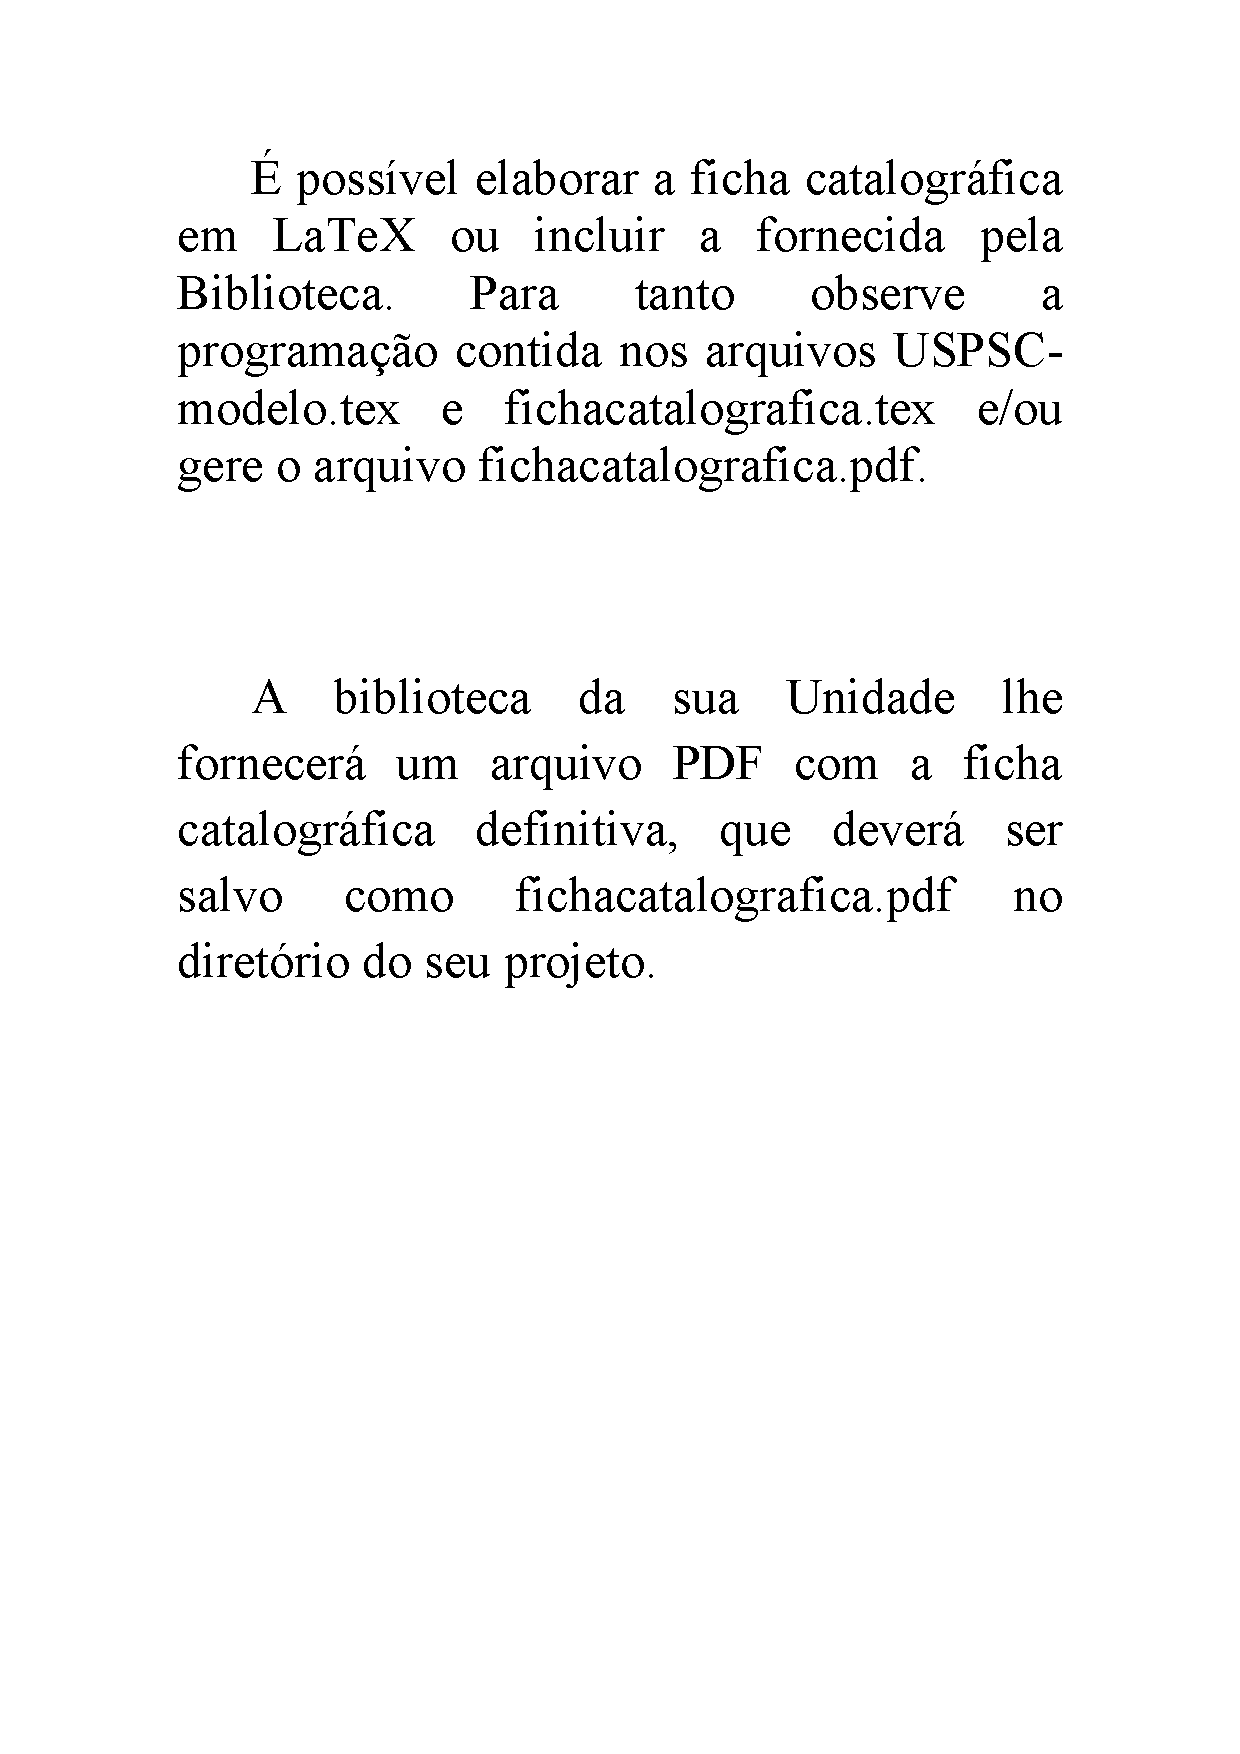
\includepdf{USPSC-TA-PreTextual/USPSC-fichacatalografica.pdf}

% Se voc\^e optar por elaborar a ficha catalogr\'afica, dever\'a 
% incluir uma % antes da linha % antes
% do comando %% USPSC-fichacatalografica.tex
% ---
% Inserir a ficha bibliografica
% ---
% Isto \'e um exemplo de Ficha Catalogr\'afica, ou ``Dados internacionais de
% cataloga\c{c}\~ao-na-publica\c{c}\~ao''. Voc\^e pode utilizar este modelo como refer\^encia. 
% Por\'em, provavelmente a biblioteca da sua universidade lhe fornecer\'a um PDF
% com a ficha catalogr\'afica definitiva ap\'os a defesa do trabalho. Quando estiver
% com o documento, salve-o como PDF no diret\'orio do seu projeto e substitua todo
% o conte\'udo de implementa\c{c}\~ao deste arquivo pelo comando abaixo:
%
\begin{fichacatalografica}
	\hspace{-1.4cm}
	\imprimirnotaautorizacao \\ \\
	%\sffamily
	\vspace*{\fill}					% Posi\c{c}\~ao vertical
\begin{center}					% Minipage Centralizado
  \imprimirnotabib \\
  \begin{table}[htb]
	\scriptsize
	\centering	
	\begin{tabular}{|p{0.9cm} p{8.7cm}|}
		\hline
	      & \\
		  &	  \imprimirautorficha     \\
		
		 \imprimircutter & 
							\hspace{0.4cm}\imprimirtitulo~  / ~\imprimirautor~ ;  ~\imprimirorientadorcorpoficha. -- 	\imprimirlocal, \imprimirdata.   \\
		
		  &  % Para incluir nota referente \`a vers\~ao corrigida no corpo da ficha,
			  % incluir % no in\'{\i}cio da linha acima e tirar a % do in\'{\i}cio da linha abaixo
			  %	\hspace{0.4cm} \imprimirtitulo~  / ~\imprimirautor~ ; ~\imprimirorientadorcorpoficha~- ~\imprimirnotafolharosto. -- \imprimirlocal, \imprimirdata.  \\
		
			\hspace{0.4cm}\pageref{LastPage} p. : il. (algumas color.) ; 30 cm.\\ 
		  & \\
		  & 
		    \hspace{0.4cm}\imprimirnotaficha ~--~ 
						  \imprimirunidademin, 
						  \imprimiruniversidademin, 
		                  \imprimirdata. \\ 
		  & \\                 
		   % Para incluir nota referente \`a vers\~ao corrigida em notas,
		    % incluir uma % no in\'{\i}cio da linha acima e	
		    % tirar a % do in\'{\i}cio da linha abaixo
		    % & \hspace{0.4cm}\imprimirnotafolharosto \\ 
		  & \\ 
		  & \hspace{0.4cm}1. LaTeX. 2. abnTeX. 3. Classe USPSC. 4. Editora\c{c}\~ao de texto. 5. Normaliza\c{c}\~ao da documenta\c{c}\~ao. 6. Tese. 7. Disserta\c{c}\~ao. 8. Documentos (elabora\c{c}\~ao). 9. Documentos eletr\^onicos. I. \imprimirorientadorficha. 
		   II. T\'{\i}tulo. \\
	
		     %Se houver co-orientador, inclua % antes da linha (antes de II. T\'{\i}tulo.) 
		     %          e tire a % antes do comando abaixo 
		     %III. T\'{\i}tulo. \\   
		  \hline
	\end{tabular}
  \end{table}
\end{center}
\end{fichacatalografica}
% ---

 
% e retirar o % do comando abaixo
%% USPSC-fichacatalograficaTutorial.tex
% ---
% Inserir a ficha bibliografica
% ---
% Isto \'e um exemplo de Ficha Catalogr\'afica, ou ``Dados internacionais de
% cataloga\c{c}\~ao-na-publica\c{c}\~ao''. Voc\^e pode utilizar este modelo como refer\^encia. 
% Por\'em, provavelmente a biblioteca da sua universidade lhe fornecer\'a um PDF
% com a ficha catalogr\'afica definitiva ap\'os a defesa do trabalho. Quando estiver
% com o documento, salve-o como PDF no diret\'orio do seu projeto e substitua todo
% o conte\'udo de implementa\c{c}\~ao deste arquivo pelo comando abaixo:

\textbf{UNIVERSIDADE DE S\~AO PAULO} 

Reitor: Vahan Agopyan

Vice-Reitor: Ant\^onio Carlos Hernandes\\

\textbf{Grupo Desenvolvedor do Pacote USPSC} 

\textbf{Coordena\c{c}\~ao e Programa\c{c}\~ao}

- Marilza Aparecida Rodrigues Tognetti (PUSP-SC)
	
- Ana Paula Aparecida Calabrez (PUSP-SC) 

\textbf{Normaliza\c{c}\~ao}

- Ana Paula Aparecida Calabrez (PUSP-SC) 

- Brianda de Oliveira Ordonho Sigolo (IAU)

- Eduardo Graziosi Silva (EESC)

- Eliana de C\'assia Aquareli Cordeiro (IQSC)

- Fl\'avia Helena Cassin (EESC)

- Maria Cristina Cavarette Dziabas (IFSC)

- Marilza Aparecida Rodrigues Tognetti (PUSP-SC)

- Regina C\'elia Vidal Medeiros (ICMC) \\


%
\begin{fichacatalografica}
%	\hspace{-1.4cm}
   \vspace*{\fill}					% Posi\c{c}\~ao vertical
\begin{center}					% Minipage Centralizado
  \imprimirnotabib \\
  \begin{table}[Htb]
	\scriptsize
	\centering	
	\begin{tabular}{|p{0.9cm} p{8.7cm}|}
		\hline
	      & \\
		  &	  \imprimirautorficha     \\
		
		 \imprimircutter & 
							\hspace{0.4cm}\imprimirtitulo~ / ~{Marilza Aparecida Rodrigues Tognetti; Ana Paula Aparecida Calabrez,  coordenadoras e progamadoras. Brianda de Oliveira Ordonho Sigolo ...[\textit{et al.}], normalizadoras}.
							 -- 	\imprimirlocal, USP, \imprimirdata.   \\
		
		  &			\hspace{0.4cm}\pageref{LastPage} p. : il. (algumas color.) ; 30 cm.\\ 
 		  & \\ 
		  & \hspace{0.4cm}1. LaTeX. 2. abnTeX. 3. Classe USPSC. 4. Editora\c{c}\~ao de texto. 5. Normaliza\c{c}\~ao da documenta\c{c}\~ao. 6. Tese. 7. Disserta\c{c}\~ao. 8. Documentos (elabora\c{c}\~ao). 9. Documentos eletr\^onicos. I. Calabrez, A. P. A., coord., program., normaliz. II. Sigolo, B. O. O. normaliz. III. Cordeiro, E. C. A., normaliz. IV. Cassin, Fl\'avia Helena, normaliz. V. Dziabas, M. C. C., normaliz. VI. Medeiros, R. C. V., normaliz.  VII. T\'{\i}tulo.  \\
	
		  \hline
	\end{tabular}
  \end{table}
\end{center}
\end{fichacatalografica}
% ---

% As informa\c{c}\~oes que comp\~oem a ficha catalogr\'afica est\~ao 
% definidas no arquivo USPSC-pre-textual-UUUU.tex
% ---

% ---
% Folha de rosto adicional
% Para imprimir a folha de rosto adicional, exigida por algumas Unidades, a exemplo do ICMC,
% retire a % antes do comando abaixo

%\imprimirfolhaderostoadic

% ---
% ---
% Inserir errata
% ---

%% USPSC-ErrataTutorial.tex
\begin{errata}
	%\OnehalfSpacing 			
	A errata é um elemento opcional, que consiste de uma lista de erros da obra, precedidos pelas folhas e linhas onde eles ocorrem e seguidos pelas correções correspondentes. Deve ser inserida logo após a folha de rosto e conter a referência do trabalho para facilitar sua identificação, conforme a ABNT NBR 14724 \cite{nbr14724}. 
	
    Em USPSC-Tutorial.tex foi utilizado o arquivo \textbf{USPSC-ErrataTutorial.tex}, pois a referência bibliográfica é compatível com o tipo deste documento que é um tutorial (monografia/livro). 
    
    Para teses, dissertações, TCCs e outros trabalhos acadêmicos utilize o arquivo \textbf{USPSC-Errata.tex}, conforme indicado em  USPSC-Modelo.tex e USPSC-TCC-modelo.tex. 
    
       
	Modelo de Errata:
		
	\begin{flushleft} 
			\setlength{\absparsep}{0pt} % ajusta o espaçamento da referência	
			\SingleSpacing 
			\imprimirautorabr.~~\textbf{\imprimirtituloresumo}.~~\imprimirorientador~~	
			%Substitua p. por f. quando utilizar oneside em \documentclass
			%\pageref{LastPage}f.
			\imprimirlocal: \imprimirinstituicao, \imprimirdata. \pageref{LastPage}p. 
 	\end{flushleft}
\vspace{\onelineskip}
\OnehalfSpacing 
\center
\textbf{ERRATA}
\vspace{\onelineskip}
\OnehalfSpacing 
\begin{table}[htb]
	\center
	\footnotesize
	\begin{tabular}{p{2cm} p{2cm} p{4cm} p{4cm} }
		\hline
		\textbf{Folha} & \textbf{Linha}  & \textbf{Onde se lê}  & \textbf{Leia-se}  \\
			\hline
			1 & 10 & auto-conclavo & autoconclavo\\
		\hline
	\end{tabular}
\end{table}
\end{errata}
% ---
%Para Teses, Disserta\c{c}\~oes, TCCs e outros trabalhos acad\^emicos, no arquivo USPSC-Modelo.tex e USPSC-TCC-modelo.tex, utilizar o comando %% USPSC-Errata.tex
\begin{errata}
	%\OnehalfSpacing 			
	A errata é um elemento opcional, que consiste de uma lista de erros da obra, precedidos pelas folhas e linhas onde eles ocorrem e seguidos pelas correções correspondentes. Deve ser inserida logo após a folha de rosto e conter a referência do trabalho para facilitar sua identificação, conforme a ABNT NBR 14724 \cite{nbr14724}.
	
	Modelo de Errata:
		
	\begin{flushleft} 
			\setlength{\absparsep}{0pt} % ajusta o espaçamento da referência	
			\SingleSpacing 
			\imprimirautorabr~ ~\textbf{\imprimirtituloresumo}.	\imprimirdata. \pageref{LastPage}p. 
			%Substitua p. por f. quando utilizar oneside em \documentclass
			%\pageref{LastPage}f.
			\imprimirtipotrabalho~-~\imprimirinstituicao, \imprimirlocal, \imprimirdata. 
 	\end{flushleft}
\vspace{\onelineskip}
\OnehalfSpacing 
\center
\textbf{ERRATA}
\vspace{\onelineskip}
\OnehalfSpacing 
\begin{table}[htb]
	\center
	\footnotesize
	\begin{tabular}{p{2cm} p{2cm} p{4cm} p{4cm} }
		\hline
		\textbf{Folha} & \textbf{Linha}  & \textbf{Onde se lê}  & \textbf{Leia-se}  \\
			\hline
			1 & 10 & auto-conclavo & autoconclavo\\
		\hline
	\end{tabular}
\end{table}
\end{errata}
% ---

% ---

% ---
% Inserir folha de aprova\c{c}\~ao
% ---

% A Folha de aprova\c{c}\~ao \'e um elemento obrigat\'orio da NBR 4724/2011 (se\c{c}\~ao 4.2.1.3). 
% Ap\'os a defesa/aprova\c{c}\~ao do trabalho, gere o arquivo folhadeaprovacao.pdf da p\'agina assinada pela banca 
% e iclua o arquivo utilizando o comando abaixo:
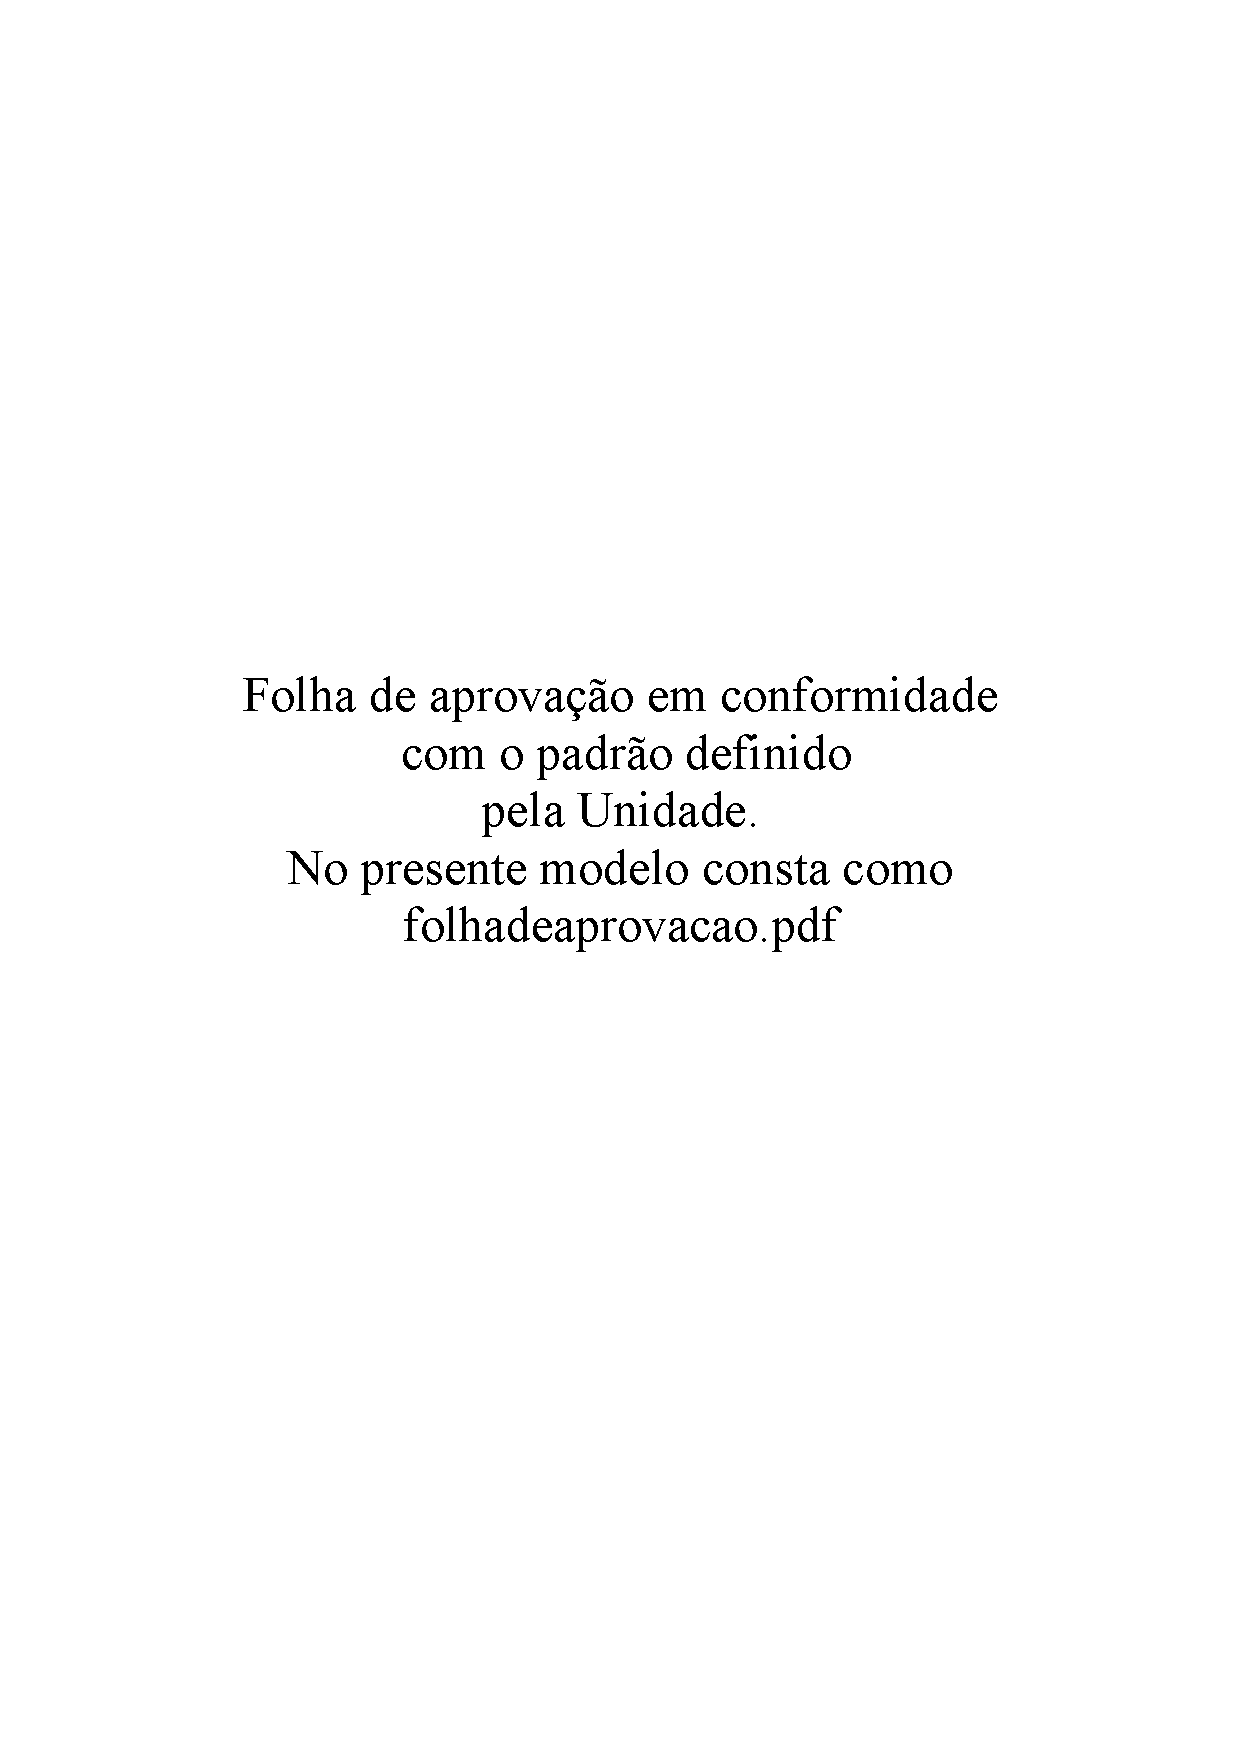
\includepdf{USPSC-TA-PreTextual/USPSC-folhadeaprovacao.pdf}
% Alternativa para a Folha de Aprova\c{c}\~ao:
% Se for a sua op\c{c}\~ao elaborar uma folha de aprova\c{c}\~ao, insira uma % antes do comando acima que inclui o arquivo folhadeaprovacao.pdf,
% tire o % do comando abaixo e altere o arquivo folhadeaprovacao.tex conforme suas necessidades
%\include{folhadeaprovacao}

\includepdf{USPSC-TA-PreTextual/USPSC-PaginaEmBranco.pdf}

% ---
% Dedicat\'oria
% ---
%% USPSC-Dedicatoria.tex
\begin{dedicatoria}
   \vspace*{\fill}
   \centering
   \noindent
   \textit{ Este trabalho \'e dedicado aos alunos da USP, como uma contribuição\\
  das Bibliotecas do Campus USP de São Carlos para o desenvolvimento\\
	e disseminação da pesquisa científica da Universidade.} \vspace*{\fill}
\end{dedicatoria}
% ---
% ---

% ---
% Agradecimentos
% ---
%% USPSC-AgradecimentosTutorial.tex
\begin{agradecimentos}
	A motivação para o desenvolvimento da classe USPSC e dos modelos de trabalhos acadêmicos foi decorrente de solicitações de usuários das Bibliotecas do Campus USP de São Carlos. A versão 3.0 do Pacote USPSC para modelos de trabalhos acadêmicos é composta da \textbf{Classe USPSC}, do \textbf{Modelo para TCC em \LaTeX\ utilizando o Pacote USPSC} e do \textbf{Modelo para teses e dissertações em \LaTeX\ utilizando o Pacote USPSC}.
	
	Nesta versão do Pacote USPSC, foram feitas alterações na Classe USPSC, inclusão da capa exclusiva para o Instituto de Ciências Matemáticas e de Computação (ICMC), inclusão de novos pacotes e alterações nos modelos de trabalhos acadêmicos.
	
	Na versão 3.0 do Pacote USPSC, as mudanças foram estruturais na programação e conteúdo. Destacamos que os modelos \textbf{USPSC-modelo.tex} e \textbf{USPSC-TCC-modelo.tex} foram simplificados, no que tange ao conteúdo, e foi criado o \textbf{Tutorial do Pacote USPSC para modelos de trabalhos de acad\^emicos em LaTeX - vers\~ao 3.0}, contendo as instruções precisas e detalhadas para melhor utilização dos recursos do Pacote USPSC. Para tanto, foram acrescidos diversos arquivos, para atender as especificidades do tutorial que possui os elementos pré-textuais distintos para teses, dissertações, TCCs e outros trabalhos acadêmicos, conforme descrito em  \textbf{\ref{Pacote} Pacote USPSC: Classe USPSC e modelos de trabalhos de acadêmicos}. A estrutura deste tutorial é igual à  estrutura de trabalhos acadêmicos estabelecida pela ABNT NBR 14724, conforme a \autoref{fig_EstruturaTrabAcad}, portanto o usuário do Pacote USPSC pode utilizar os exemplos e recursos de \LaTeX\ nele contidos.	
	 
	Na versão 3.1 houve a inclusão da capa diferenciada para o Instituto de Ciências Matemáticas e de Computação (ICMC), novos cursos e programas e de algumas alterações na Classe USPSC, arquivos USPSC.cls e  USPSC1.cls.
	
	O Grupo desenvolvedor do Pacote USPSC agradece especialmente ao Luis Olmes, doutorando do ICMC, pelas primeiras orientações sobre o \LaTeX\ . 
	
	Agradecemos ao Lauro César Araujo pelo desenvolvimento da classe  \abnTeX, modelos canônicos e tantas outras contribuições que nos permitiu o desenvolvimento o Pacote USPSC, composto da classe USPSC e seus modelos.
	
	Os nossos agradecimentos aos integrantes do primeiro
	projeto abn\TeX\, Gerald Weber, Miguel Frasson, Leslie H. Watter, Bruno Parente Lima, Flávio de Vasconcellos Corrêa, Otavio Real
	Salvador, Renato Machnievscz, e a todos que contribuíram para que a produção de trabalhos acadêmicos em conformidade com
	as normas ABNT com \LaTeX\ fosse possível.
	
	Agradecemos ao grupo de usuários
	\emph{latex-br}  {\url{http://groups.google.com/group/latex-br}}, aos integrantes do grupo
	\emph{\abnTeX}  {\url{http://groups.google.com/group/abntex2}  e \url{http://www.abntex.net.br/}}~que contribuem para a evolução do \abnTeX.
	
	Agradecemos aos usuários do Pacote USPSC que nos tem dado um \textit{feedback} e sugestões de melhoria. 
	
\end{agradecimentos}
% ---
% ---

% ---
% Ep\'{\i}grafe
% ---
%% USPSC-EpigrafeTutorial.tex
\begin{epigrafe}
    \vspace*{\fill}
	\begin{flushright}
		\textit{``O estudo, a busca da verdade e da beleza são domínios \\
		em que nos \'e consentido sermos crianças por toda a vida.''\\
		Albert Einstein}
	\end{flushright}
\end{epigrafe}
% ---
% ---

% A T E N \c{C} \~A O
% Se o idioma do texto for em ingl\^es, o abstract deve preceder o resumo
% resumo em portugu\^es
%
% Resumo
% ---
%% USPSC-ResumoTutorial.tex
\setlength{\absparsep}{18pt} % ajusta o espa\c{c}amento dos par\'agrafos do resumo		
\begin{resumo}
	\begin{flushleft} 
		\setlength{\absparsep}{0pt} % ajusta o espa\c{c}amento da refer\^encia	
		\SingleSpacing 
		\imprimirautorabr.~~\textbf{\imprimirtituloresumo}.~~\imprimirorientador~~	
		%Substitua p. por f. quando utilizar oneside em \documentclass
		%\pageref{LastPage}f.
		\imprimirlocal: \imprimirinstituicao, \imprimirdata. \pageref{LastPage}p. 
	\end{flushleft}
\OnehalfSpacing 			
 O resumo deve ressaltar o  objetivo, o m\'etodo, os resultados e as conclus\~oes do documento. A ordem e a extens\~ao  destes itens dependem do tipo de resumo (informativo ou indicativo) e do  tratamento que cada item recebe no documento original. O resumo deve ser
 precedido da refer\^encia do documento, com exce\c{c}\~ao do resumo inserido no
 pr\'oprio documento. (\ldots)  Salientamos que algumas Unidades exigem o titulo dos trabalhos acad\^emicos em ingl\^es, tornando necess\'ario a inclus\~ao das refer\^encias nos resumos e abstracts, o que foi adotado no \textbf{Modelo para TCC em \LaTeX\ utilizando o Pacote USPSC} e no \textbf{Modelo para teses e disserta\c{c}\~oes em \LaTeX\ utilizando o Pacote USPSC}. As palavras-chave devem figurar logo abaixo do  resumo, antecedidas da express\~ao Palavras-chave:, separadas entre si por  ponto e finalizadas tamb\'em por ponto \cite{nbr6028}.
 

 \textbf{Palavras-chave}: LaTeX. abnTeX. Classe USPSC. Editora\c{c}\~ao de texto. Normaliza\c{c}\~ao da documenta\c{c}\~ao. Trabalho acad\^emico. Tese. Disserta\c{c}\~ao. Trabalho de conclus\~ao de curso (TCC). Documentos (elabora\c{c}\~ao). Documentos eletr\^onicos. 
\end{resumo}
% ---

% Abstract
% ---
%% USPSC-AbstractTutorial.tex
%\autor{Silva, M. J.}
\begin{resumo}[Abstract]
 \begin{otherlanguage*}{english}
   \begin{flushleft} 
   	\setlength{\absparsep}{0pt} % ajusta o espa\c{c}amento da refer\^encia	
   	\SingleSpacing 
   	\imprimirautorabr.~~\textbf{\imprimirtitleabstract}.~~\imprimirorientador~~	
   	%Substitua p. por f. quando utilizar oneside em \documentclass
   	%\pageref{LastPage}f.
   	\imprimirlocal: \imprimirinstituicao, \imprimirdata. \pageref{LastPage}p. 
   \end{flushleft}
	\OnehalfSpacing 
   This is the english abstract.

   \vspace{\onelineskip}
 
   \noindent 
   \textbf{Keywords}: LaTeX. abnTeX. USPSC class. Text editoration. Standardization of documentation. Academic work. Thesis. Dissertation. Conclusion course paper. Documents (development). Electronic documents.
   \end{otherlanguage*}
\end{resumo}

% ---

% ---
% inserir lista de figurass
% ---
\pdfbookmark[0]{\listfigurename}{lof}
\listoffigures*
\cleardoublepage
% ---

% ---
% inserir lista de tabelas
% ---
\pdfbookmark[0]{\listtablename}{lot}
\listoftables*
\cleardoublepage
% ---

% ---
% inserir lista de quadros
% ---
\pdfbookmark[0]{\listofquadroname}{loq}
\listofquadro*
\cleardoublepage
% ---

% ---
% inserir lista de abreviaturas e siglas
% ---
% USPSC-AbreviaturasSiglasTutorial.tex
\begin{siglas}
    \item[ABNT] Associação Brasileira de Normas T\'ecnicas
    \item[abnTeX] ABsurdas Normas para TeX
	\item[EESC] Escola de Engenharia de São Carlos
	\item[IAU] Instituto de Arquitetura e Urbanismo
	\item[IBGE] Instituto Brasileiro de Geografia e Estatística
	\item[ICMC] Instituto de Ci\^encias Matem\'aticas e de Computação
	\item[IFSC] Instituto de Física de São Carlos
	\item[IQSC] Instituto de Química de São Carlos
	\item[LaTeX] Lamport TeX
	\item[PDF] Portable Document Format
	\item[PUSP-SC] Prefeitura do Campus USP de São Carlos
	\item[TCC] Trabalho de Conclusão de Curso
	\item[USP] Universidade de São Paulo
	\item[USPSC] Campus USP de São Carlos
\end{siglas}

% ---

% ---
% inserir lista de s\'{\i}mbolos
% ---
% USPSC-SimbolosTutorial.tex
\begin{simbolos}
  \item[$ \Gamma $] Letra grega Gama
  \item[$ \Lambda $] Lambda
  \item[$ \zeta $] Letra grega minúscula zeta
  \item[$ \in $] Pertence
\end{simbolos}
% ---
% ---
% inserir o sumario
% ---
\pdfbookmark[0]{\contentsname}{toc}
\tableofcontents*
\cleardoublepage
% ---
% ----------------------------------------------------------
% ELEMENTOS TEXTUAIS
% ----------------------------------------------------------
\textual
% Os cap\'{\i}tulos s\~ao inseridos como arquivos externos 

% Cap\'{\i}tulo 1 - Introdu\c{c}\~ao
% ---
%% USPSC-IntroducaoTutorial.tex

% ----------------------------------------------------------
% Introdu\c{c}\~ao (exemplo de cap\'{\i}tulo sem numera\c{c}\~ao, mas presente no Sum\'ario)
% ----------------------------------------------------------
\chapter[Introdu\c{c}\~ao]{Introdu\c{c}\~ao}
\label{Introdu\c{c}\~ao}

Parte inicial do texto, que cont\'em a delimita\c{c}\~ao do assunto tratado, objetivos da pesquisa e outros elementos necess\'arios para apresentar o tema do trabalho \cite{aguia2020}.

A equipe de desenvolvimento e manuten\c{c}\~ao do Pacote USPSC, atualmente na vers\~ao 3.1, contendo a Classes USPSC, tutorial e modelos para trabalhos acad\^emicos em \LaTeX\ utilizando a classe USPSC, foi estabelecida em abril de 2015. \'E integralmente composta por pessoas vinculadas \`as Bibliotecas das Unidades de ensino e pesquisa do Campus USP de S\~ao Carlos, incluindo a Biblioteca da Prefeitura do Campus USP de S\~ao Carlos (PUSP-SC), para garantir a sustentabilidade deste produto, tendo autonomia para implementar novos recursos, efetuar compatibiliza\c{c}\~oes necess\'arias em decorr\^encia de altera\c{c}\~oes de normas da ABNT e/ou normas e padr\~oes estabelecidos pelas comiss\~oes de p\'os-gradua\c{c}\~ao das Unidades, incluir novos programas de p\'os-gradua\c{c}\~ao das Unidades, dentre outras raz\~oes.

O Grupo Desenvolvedor do Pacote USPSC optou por manter os exemplos apresentados nas vers\~oes anteriores do tutorial, que s\~ao os relacionados no cap\'{\i}tulo \textbf{\ref{Refer\^encias} MODELOS DE REFER\^ENCIAS} do documento \textbf{Diretrizes para apresenta\c{c}\~ao de disserta\c{c}\~oes e teses da USP}: documento eletr\^onico e impresso - Parte I (ABNT), 3ª edi\c{c}\~ao de 2016, por\'em em conformidade com ABNT NBR 6023:2018. 

Atualmente a USP em S\~ao Carlos possui a Prefeitura do Campus USP de S\~ao Carlos (PUSP-SC), o Centro de Divulga\c{c}\~ao Cient\'{\i}fica e Cultural (CDCC) e as seguintes Unidades de ensino e pesquisa: Escola de Engenharia de S\~ao Carlos (EESC), @[unidadefaculdade]@, @[unidadefaculdade]@, @[unidadefaculdade]@.

Na vers\~ao 2.0 o Pacote USPSC passou a ser composto pela \textbf{Classe USPSC}, o \textbf{Modelo para TCC em \LaTeX\ utilizando a classe USPSC} e o \textbf{Modelo para teses e disserta\c{c}\~oes em \LaTeX\ utilizando a classe USPSC} para a EESC.

Na vers\~ao 3.0 do Pacote USPSC os modelos de trabalhos acad\^emicos \textbf{USPSC-modelo.tex} e \textbf{USPSC-TCC-modelo.tex} foram simplificados, no que tange ao conte\'udo, e foi criado o \textbf{Tutorial do Pacote USPSC para modelos de trabalhos de acad\^emicos em LaTeX - vers\~ao 3.0}, contendo as instru\c{c}\~oes precisas e detalhadas para melhor utiliza\c{c}\~ao dos recursos do Pacote USPSC. Para tanto, foram acrescidos diversos arquivos, para atender as especificidades do tutorial que possui os elementos pr\'e-textuais distintos para teses, disserta\c{c}\~oes, TCCs e outros trabalhos acad\^emicos, conforme descrito em  \textbf{\ref{Pacote} Pacote USPSC: Classe USPSC e modelos de trabalhos de acad\^emicos}. A estrutura deste tutorial \'e igual \`a  estrutura de trabalhos acad\^emicos estabelecida pela ABNT NBR 14724, conforme a \autoref{fig_EstruturaTrabAcad}.		

A vers\~ao 3.0 do Pacote USPSC traz ainda as seguintes altera\c{c}\~oes e implementa\c{c}\~oes:

\begin{alineas}	 
	\item foi alterada a estrutura da pasta para distribuir mais didaticamente os diversos arquivos que comp\~oem o referido pacote, conforme descrito em \ref{Pacote}; 
	\item foram criados os seguintes arquivos de elementos pr\'e-textuais: USPSC-Errata.tex, USPSC-Dedicatoria.tex, USPSC-Agradecimentos.tex, USPSC-Epigrafe.tex,\\
	USPSC-Resumo.tex, USPSC-Abstract.tex, USPSC-AbreviaturasSiglas.tex e USPSC-Simbolos.tex. 
	Tais informa\c{c}\~oes constavam diretamente dos arquivos \textbf{USPSC-modelo.tex} e  \textbf{USPSC-TCC-modelo.tex} e nesta vers\~ao passaram a ser inclu\'{\i}das atrav\'es do comando \verb+\include{nome do arquivo tex}+;
	\item implementa\c{c}\~ao do Modelo para TCC para o ICMC e IQSC, conforme descrito em \ref{Pacote};
	\item altera\c{c}\~ao do pacote utilizado para estruturas, rea\c{c}\~oes e mecanismos de rea\c{c}\~oes qu\'{\i}micas, conforme descrito em \ref{Reaquimica};
	\item altera\c{c}\~oes na Classe USPSC (USPSC.cls e USPSC1.cls):
		\begin{subalineas}
			\item foi adicionado o comando \verb+\ABNTEXcaptiondelim+ e alterado o separador de \textbf{captions} para \textbf{long dash} visando a compatibiliza\c{c}\~ao com a norma  ABNT NBR 14724:2011 e a conformidade com a classe \abnTeX\ v1.9.6;
			\item para incluir novos comandos e par\^ametros para possibilitar a impress\~ao de p\'agina de rosto adicional, atualmente adotada apenas pelo ICMC;
		\end{subalineas}
	\item altera\c{c}\~oes no arquivo USPSC-pre-textual-EESC.tex em decorr\^encia das altera\c{c}\~oes nos programas de p\'os-gradua\c{c}\~ao;
	\item altera\c{c}\~oes no arquivo USPSC-pre-textual-IFSC.tex para incluir op\c{c}\~oes de programas em ingl\^es;
	\item altera\c{c}\~oes no arquivo USPSC-pre-textual-ICMC.tex para incluir os comandos e par\^ametros referentes \`a p\'agina de rosto adicional;
	\item altera\c{c}\~oes no arquivo USPSC-Unidades.tex para incluir os comandos relativos aos novos Modelos de TCC;
	\item cria\c{c}\~ao dos arquivos USPSC-TCC-pre-textual-ICMC.tex e USPSC-TCC-pre-textual-IQSC.tex, necess\'arios para implementar o Modelo para TCC para o ICMC e IQSC;
	\item altera\c{c}\~ao no cap\'{\i}tulo \textbf{\ref{Refer\^encias} MODELOS DE REFER\^ENCIAS}, mantendo os exemplos contidos nas \textbf{Diretrizes para apresenta\c{c}\~ao de disserta\c{c}\~oes e teses da USP}: documento eletr\^onico e impresso - Parte I (ABNT), por\'em em conformidade com ABNT NBR 6023:2018; 
	\item inclus\~ao da alternativa de cores para os links nos arquivos \textbf{USPSC-modelo.tex} e \textbf{USPSC-TCC-modelo.tex}, conforme descrito em \ref{coreslinks} 
	\item altera\c{c}\~oes no arquivo \textbf{USPSC-modelo.tex} e nos demais arquivos \textbf{.tex} em conformidade com as altera\c{c}\~oes e implementa\c{c}\~oes efetuadas.	\\
\end{alineas}

	A vers\~ao 3.1 traz as altera\c{c}\~oes na Classe USPSC (USPSC.cls e USPSC1.cls) espec\'{\i}ficas para incluir novos par\^ametros para capa e tipo de publica\c{c}\~ao em ingl\^es.

	O Grupo Desenvolvedor do Pacote USPSC est\'a assim constitu\'{\i}do:

\textbf{Coordena\c{c}\~ao e Programa\c{c}\~ao}

- Marilza Aparecida Rodrigues Tognetti - marilza@sc.usp.br (PUSP-SC)	

- Ana Paula Aparecida Calabrez - aninha@sc.usp.br (PUSP-SC) 

\textbf{Normaliza\c{c}\~ao e Padroniza\c{c}\~ao}

- Ana Paula Aparecida Calabrez - aninha@sc.usp.br (PUSP-SC)

- Brianda de Oliveira Ordonho Sigolo - brianda@usp.br (IAU)

- Eduardo Graziosi Silva - edu.gs@sc.usp.br (EESC)

- Eliana de C\'assia Aquareli Cordeiro - eliana@iqsc.usp.br (IQSC)

- Fl\'avia Helena Cassin - cassinp@sc.usp.br (EESC)	

- Maria Cristina Cavarette Dziabas - mcdziaba@ifsc.usp.br (IFSC)	

- Marilza Aparecida Rodrigues Tognetti - marilza@sc.usp.br (PUSP-SC)

- Regina C\'elia Vidal Medeiros - rcvm@icmc.usp.br (ICMC)

	O objetivo do presente trabalho \'e apresentar a vers\~ao 3.1 do Pacote USPSC, composto pela \textbf{Classe USPSC}, \textbf{Tutorial do Pacote USPSC para modelos de trabalhos de acad\^emicos em LaTeX - vers\~ao 3.1},  \textbf{Modelo para TCC em \LaTeX\ utilizando a classe USPSC} e o \textbf{Modelo para teses e disserta\c{c}\~oes em \LaTeX\ utilizando a classe USPSC}, concebidos em conformidade com a \textbf{ABNT NBR 14724} \cite{nbr14724}, as \textbf{Diretrizes para apresenta\c{c}\~ao de disserta\c{c}\~oes e teses da USP} \cite{aguia2020} e normas e padr\~oes estabelecidos pelas Unidades. 
	
	A expectativa \'e que o Pacote USPSC, mediante os modelos propostos, proporcione o aprimoramento da qualidade dos trabalhos acad\^emicos produzidos pelos alunos de gradua\c{c}\~ao e de p\'os-gradua\c{c}\~ao das referidas Unidades de Ensino e Pesquisa do Campus USP de S\~ao Carlos, garantindo a normaliza\c{c}\~ao e padroniza\c{c}\~ao estabelecidas.
	
	
% ---

% ---
% Cap\'{\i}tulo 2
% ---
%% USPSC-Cap2-DesenvolvimentoTutorial.tex 

% ---
% Este cap\'{\i}tulo, utilizado por diferentes exemplos do abnTeX2, ilustra o uso de
% comandos do abnTeX2 e de LaTeX.
% ---

\chapter{Desenvolvimento}\label{cap_exemplos}
Este cap\'{\i}tulo \'e parte principal do trabalho acad\^emico e deve conter a exposi\c{c}\~ao ordenada e detalhada do assunto. Divide-se em se\c{c}\~oes e subse\c{c}\~oes, em conformidade com a abordagem do tema e do m\'etodo, abrangendo: revis\~ao bibliogr\'afica, materiais e m\'etodos, t\'ecnicas utilizadas, resultados obtidos e discuss\~ao.

O conte\'udo deste documento visa apresentar um tutorial para utiliza\c{c}\~ao do Pacote USPSC, composto da Classe USPSC, tutorial e modelos, utilizando a estrutura de trabalhos acad\^emicos, mas por quest\~oes did\'aticas adotou-se cap\'{\i}tulo, se\c{c}\~oes e subse\c{c}\~oes diferentes das usualmente utilizadas.


\section{Pacote USPSC: Classe USPSC e modelos de trabalhos acad\^emicos}\label{Pacote}
A vers\~ao 3.1 do Pacote USPSC traz os modelos simplificados de trabalhos acad\^emicos \textbf{USPSC-modelo.tex} e \textbf{USPSC-TCC-modelo.tex} e o \textbf{Tutorial do Pacote USPSC para modelos de trabalhos acad\^emicos em LaTeX - vers\~ao 3.1}, contendo as instru\c{c}\~oes precisas e detalhadas para melhor utiliza\c{c}\~ao dos recursos do Pacote USPSC. Para tanto, foram acrescidos diversos arquivos, para atender as especificidades do tutorial que possui os elementos pr\'e-textuais distintos para teses, disserta\c{c}\~oes, TCCs e outros trabalhos acad\^emicos, conforme descrito em  \textbf{\ref{Pacote} Pacote USPSC: Classe USPSC e modelos de trabalhos acad\^emicos}. A estrutura deste tutorial \'e igual \`a estrutura de trabalhos acad\^emicos estabelecida pela ABNT NBR 14724, conforme a \autoref{fig_EstruturaTrabAcad}.

Todas as altera\c{c}\~oes e novas implementa\c{c}\~oes foram relacionadas em \textbf{\ref{Introdu\c{c}\~ao} INTRODU\c{C}\~AO} e neste cap\'{\i}tulo ser\~ao descritas detalhadamente, quando necess\'ario. 

A classe USPSC \'e uma derivada da classe \textbf{\abnTeX\ v1.9.5} para as Unidades de ensino e pesquisa do Campus USP de S\~ao Carlos:
Escola de Engenharia de S\~ao Carlos (EESC), @[unidadefaculdade]@, @[unidadefaculdade]@\^encias Matem\'aticas e de Computa\c{c}\~ao (ICMC), @[unidadefaculdade]@\'{\i}sica de S\~ao Carlos (IFSC) e @[unidadefaculdade]@\'{\i}mica de S\~ao Carlos (IQSC).

O objetivo do projeto \'e disponibilizar modelos em \LaTeX\  para a elabora\c{c}\~ao de trabalhos acad\^emicos (tese, disserta\c{c}\~ao, trabalho de conclus\~ao de curso (TCC), dentre outros) em conformidade com a \textbf{ABNT NBR 14724}: informa\c{c}\~ao e documenta\c{c}\~ao: trabalhos acad\^emicos: apresenta\c{c}\~ao \cite{nbr14724}, \textbf{Diretrizes para apresenta\c{c}\~ao de disserta\c{c}\~oes e teses da USP}: documento eletr\^onico e impresso - Parte I (ABNT) \cite{aguia2020} e normas e padr\~oes estabelecidos pelas Unidades.

Este documento e seu c\'odigo fonte s\~ao exemplos de uso da \textbf{Classe USPSC} e do pacote \textbf{abntex2cite}.
Para complementar as instru\c{c}\~oes contidas neste documento, utilize os manuais \cite{abnetxclasse,abnetxcite,abnetxcitealf} e da classe \textsf{memoir}\cite{memoir2010}. 


Os referidos modelos seguem a estrutura de trabalhos acad\^emicos estabelecida pela ABNT NBR 14724, conforme a \autoref{fig_EstruturaTrabAcad}. 

\begin{figure}[Htb]
	\caption{\label{fig_EstruturaTrabAcad}Estrutura do trabalho acad\^emico}
	\begin{center}
		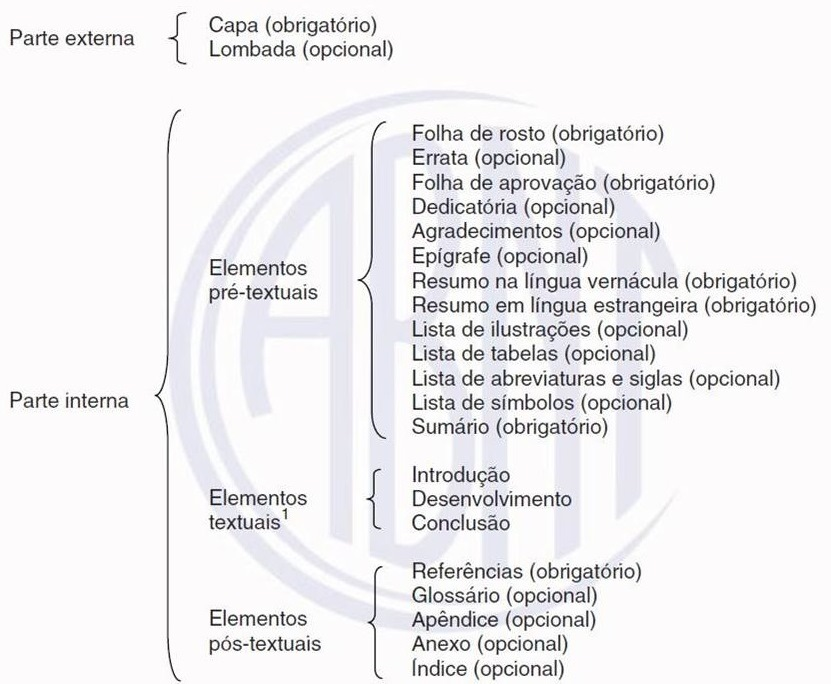
\includegraphics[scale=0.5]{USPSC-img/USPSC-EstruturaTrabAcad.jpg}
	\end{center}
	\legend{Fonte: \citeonline{nbr14724}}
\end{figure}

A vers\~ao v.3.1 do Pacote USPSC, por \textit{default}, \'e instalado em uma pasta denominada USPSC-v3.1 com a seguinte distribui\c{c}\~ao dos arquivos utilizados para gerar o documento em formato PDF, mediante a compila\c{c}\~ao utilizando um dos editores \LaTeX\ :


\begin{alineas}	
	\item \verb+ ...\USPSC-v3.1\ + contendo:	
		\begin{alineas}
			\item arquivo principal do tutorial: USPSC-tutorial.tex;
			\item arquivos principais do modelo para teses e disserta\c{c}\~oes:
				\begin{subalineas}
					\item USPSC-modelo.tex;
					\item USPSC-modelo-EESC.tex;
					\item USPSC-modelo-IAU.tex;
					\item USPSC-modelo-ICMCe.tex (idioma do texto em ingl\^es);
					\item USPSC-modelo-ICMCp.tex (idioma do texto em portugu\^es);
					\item USPSC-modelo-IFSCe.tex (idioma do texto em ingl\^es);
					\item USPSC-modelo-IFSCp.tex (idioma do texto em portugu\^es);
					\item USPSC-modelo-IQSC.tex;
				\end{subalineas}
			\item arquivos principais do modelo para TCC: 
			\begin{subalineas}
				\item USPSC-TCC-modelo.tex;
				\item USPSC-TCC-modelo-EESC.tex;
				\item USPSC-TCC-modelo-ICMCe.tex (idioma do texto em ingl\^es);
				\item USPSC-TCC-modelo-ICMCp.tex (idioma do texto em portugu\^es);
				\item USPSC-TCC-modelo-IQSC.tex;
			\end{subalineas}
			\item arquivo que relaciona os arquivos pr\'e-textuais dos programas de P\'os-Gradua\c{c}\~ao e TCCs das Unidades: USPSC-unidades.tex;
			\item arquivos pr\'e-textuais: USPSC-pre-textual-UUUU.tex e USPSC-TCC-pre-textual-UUUU.tex;
			\item pastas especificadas nos itens abaixo;
	   	\end{alineas}
	   	
	\item \verb+ ...\USPSC-v3.1\USPSC-bib\ + com o arquivo de dados das cita\c{c}\~oes e refer\^encias utilizadas: 
		\begin{alineas}	
			\item USPSC-modelo-references.bib;
		\end{alineas} 
		
	\item \verb+ ...\USPSC-v3.1\USPSC-classe\ + com os arquivos da classe USPSC, incluindo os referentes \`a compatibiliza\c{c}\~ao com a ABNT NBR 6023:2018:
		\begin{alineas}
			\item USPSC.cls;
			\item USPSC1.cls; 
			\item arquivo ABNT6023-2018.sty, para tirar <> da URL, chamado mediante o comando  \verb+ \usepackage{USPSC-classe/ABNT6023-2018}+;
			\item as demais compatibiliza\c{c}\~oes est\~ao nos arquivos abntex2-alf-USPSC.bst, abntex2-alfeng-USPSC.bst, abntex2-num-USPSC.bst e abntex2-numeng-USPSC.bst, chamados atrav\'es do comando \newline \verb+\bibliographystyle{USPSC-classe/abntex2-alf-USPSC} + ou \newline
			\verb+\bibliographystyle{USPSC-classe/abntex2-alfeng-USPSC} + ou \newline
			\verb+\bibliographystyle{USPSC-classe/abntex2-num-USPSC}+ ou \newline \verb+\bibliographystyle{USPSC-classe/abntex2-numeng-USPSC}+, dependendo se o Sistemas de chamada for autor-data ou num\'erico; 
		\end{alineas}	
	    
	\item \verb+ ...\USPSC-v3.1\USPSC-Tutorial\ + contendo:
		\begin{subalineas}
			\item USPSC-fichacatalograficaTutorial.tex;
			\item USPSC-ErrataTutorial.tex;
			\item USPSC-DedicatoriaTutorial.tex;
			\item USPSC-AgradecimentosTutorial.tex;
			\item USPSC-EpigrafeTutorial.tex;
			\item USPSC-ResumoTutorial.tex;
			\item USPSC-AbstractTutorial.tex;
			\item USPSC-AbreviaturasSiglasTutorial.tex;
			\item USPSC-SimbolosTutorial.tex;
			\item USPSC-Cap1-IntroducaoTutorial.tex;
			\item USPSC-Cap2-DesenvolvimentoTutorial;
			\item USPSC-Cap3-CitacoesTutorial.tex;
			\item USPSC-Cap4-ReferenciasTutorial.tex;
			\item USPSC-Cap5-ConclusaoTutorial.tex;
			\item USPSC-ApendicesTutorial.tex;
			\item USPSC-AnexosTutorial.tex;
			\item USPSC-IndicesRemissivosTutorial.tex.
		\end{subalineas}
	
	\item \verb+ ...\USPSC-v3.1\USPSC-TA-PreTextual\ + com os arquivos relativos aos elementos pr\'e-textuais de trabalhos acad\^emicos:
		\begin{alineas}
				\item USPSC-CapaICMC.tex;
				\item USPSC-fichacatalografica.tex;
				\item USPSC-fichacatalografica.pdf;
				\item USPSC-folhadeaprovacao.tex;
				\item USPSC-folhadeaprovacao.pdf;
				\item USPSC-Errata.tex;
				\item USPSC-Dedicatoria.tex;
				\item USPSC-Agradecimentos.tex;
				\item USPSC-Epigrafe.tex;
				\item USPSC-Resumo.tex;
				\item USPSC-Abstract.tex;
				\item USPSC-AbreviaturasSiglas.tex
				\item USPSC-Simbolos.tex 
				\item USPSC-PaginaEmBranco.pdf
			\end{alineas}
			
	\item \verb+ ...\USPSC-v3.1\USPSC-TA-Textual\ + contendo os arquivos relativos aos elementos textuais de trabalhos acad\^emicos:
		\begin{alineas}
			\item USPSC-Cap1-Introducao.tex;
			\item USPSC-Cap2-Desenvolvimento.tex;
			\item USPSC-Cap3-Conclusao.tex;
		\end{alineas}
		
	\item \verb+ ...\USPSC-v3.1\USPSC-TA-PosTextual\ + para os arquivos relativos aos elementos p\'os-textuais de trabalhos acad\^emicos:	
		\begin{alineas}
			\item USPSC-Apendices.tex;
			\item USPSC-Anexos.tex;
			\item USPSC-IndicesRemissivos.tex;
		\end{alineas}
	
	\item \verb+ ...\USPSC-v3.1\USPSC-img\ + contendo os arquivos de imagens e os PDFs relacionados no texto dos modelos: 
		\begin{alineas}	
			\item USPSC-AcentuacaoLaTeX.png;
			\item CapaICMC.jpg;
			\item USPSC-EstruturaTrabAcad.jpg;
			\item USPSC-LetrasGregas.png;
			\item USPSC-modelo-img-grafico.pdf;
			\item USPSC-modelo-img-marca.pdf;
			\item USPSC-SimbolosUteis.png;
		\end{alineas}	
	
	\item \verb+ ...\USPSC-v3.1\USPSC-Siglas\ + traz os arquivos que relacionam as siglas das Unidades e as definidas para os cursos de gradua\c{c}\~ao e programas de p\'os-gradua\c{c}\~ao, que n\~ao necessariamente s\~ao as oficiais utilizadas pela Universidade: 
		\begin{alineas}	
			\item USPSC-Siglas estabelecidas para os Programas de P\'os-Gradua\c{c}\~ao por Unidade.xlsx;
			\item USPSC-TCC-Siglas estabelecidas para as Gradua\c{c}\~oes por Unidade.xlsx;
		\end{alineas}
		
	\item \verb+ ...\USPSC-v3.1\USPSC-Sobre\ + cont\'em arquivos sobre cada vers\~ao do Pacote USPSC.

\end{alineas}	 

		
Para tese ou disserta\c{c}\~ao dever\'a ser utilizado o arquivo USPSC-modelo.tex, onde o autor dever\'a indicar a sigla da Unidade e a sigla do programa de p\'os-gradua\c{c}\~ao que est\'a vinculado, a exemplo dos comandos abaixo:
		
			\begin{verbatim}
				\siglaunidade{IQSC}
				\programa{MQOB}
			\end{verbatim}
			
Para o \textbf{Modelo para teses e disserta\c{c}\~oes em \LaTeX\ utilizando o Pacote USPSC} est\~ao definidos os seguintes arquivos pr\'e-textuais:
			
			\begin{alineas}	 
				\item USPSC-pre-textual-EESC.tex;
				\item USPSC-pre-textual-IAU.tex;
				\item USPSC-pre-textual-ICMC.tex;
				\item USPSC-pre-textual-IFSC.tex;
				\item USPSC-pre-textual-IQSC.tex.
			\end{alineas}
			
Para TCC dever\'a ser utilizado o arquivo USPSC-TCC-modelo.tex, onde o autor dever\'a indicar a \textbf{'sigla da Unidade'} + \textbf{'-TCC'} (Exemplo: EESC-TCC) e a sigla do curso de gradua\c{c}\~ao que est\'a vinculado, a exemplo dos comandos abaixo:
			
			\begin{verbatim}
			\siglaunidade{EESC-TCC}
			\programa{EAMB}
			\end{verbatim}
			
Atualmente est\~ao dispon\'{\i}veis os dados pr\'e-textuais para a EESC, ICMC e IQSC:
			
			\begin{alineas}	 
				\item USPSC-TCC-pre-textual-EESC.tex;
				\item USPSC-TCC-pre-textual-ICMC.tex;
				\item USPSC-TCC-pre-textual-IQSC.tex.
			\end{alineas}
			
Ser\~ao inclu\'{\i}dos os demais arquivos quando as demais Unidades do Campus USP de S\~ao Carlos estabelecerem seus padr\~oes. 
			
Para utilizar corretamente os dados pr\'e-textuais, \'e necess\'ario consultar as siglas estabelecidas para os cursos de gradua\c{c}\~ao e para os programas de p\'os-gradua\c{c}\~ao da Unidade de v\'{\i}nculo nos quadros dos \textbf{AP\^ENDICES B-I} ou nas planilhas \textbf{USPSC-TCC-Siglas estabelecidas para as Gradua\c{c}\~oes por Unidade.xlsx} e \textbf{USPSC-Siglas estabelecidas para os programas de p\'os-gradua\c{c}\~ao por Unidade.xlsx}. 

Os arquivos com dados pre-textuais est\~ao nominados como USPSC-pre-textual-UUUU.tex ou USPSC-TCC-pre-textual-UUUU.tex, onde UUUU \'e a sigla da Unidade. Inicialmente est\~ao disponibilizados apenas os pr\'e-textuais das Unidades do Campus USP de S\~ao Carlos.
			
Foram definidos os arquivos USPSC-pre-textual-OUTRO.tex e USPSC-TCC-pre-textual-OUTRO.tex que ser\~ao executados quando uma das siglas for diferente das explicitadas para as Unidades e/ou para os cursos de gradua\c{c}\~ao e/ou para os programas de P\'os-Gradua\c{c}\~ao. O pre\^ambulo ser\'a incompleto e apresentando "..." no final, evidenciando que o autor dever\'a rever as siglas utilizadas.

Atrav\'es do comando \verb+ %% USPSC-unidades.tex
% Camando para definição do programa de Pós-Graduação, Especialidade do Título e Instituição
\newcommand{\siglaunidade}[1]{


% EESC-TCC ==========================================================================
    \ifthenelse{\equal{#1}{EESC-TCC}}{
     			%% USPSC-TCC-pre-textual-EESC.tex
%% Camandos para defini��o do tipo de documento (tese ou disserta��o), �rea de concentra��o, op��o, pre�mbulo, titula��o 
%% referentes aos Programas de P�s-Gradua��o
\instituicao{@[unidadefaculdade]@, @[universidade]@}
\unidade{@[unidadefaculdademaiuscula]@}
\unidademin{@[unidadefaculdade]@}
\universidademin{@[universidade]@}
% A EESC n�o inclui a nota "Vers�o original", portanto o comando abaixo n�o tem a mensagem entre {}
\notafolharosto{ }
%Para a vers�o corrigida tire a % do comando/declara��o abaixo e inclua uma % antes do comando acima
%\notafolharosto{VERS\~AO CORRIGIDA}
% ---
% dados complementares para CAPA e FOLHA DE ROSTO
% ---
\universidade{@[universidademaiuscula]@}
\titulo{@[titulo]@}
\titleabstract{@[tituloabstract]@}
\tituloresumo{@[titulo]@}
\autor{@[autor]@}
\autorficha{@[autorficha]@}
\autorabr{@[autorabr]@}

\cutter{S856m}
% Para gerar a ficha catalogr�fica sem o C�digo Cutter, basta 
% incluir uma % na linha acima e tirar a % da linha abaixo
%\cutter{ }

\local{@[localidade]@}
\data{@[ano]@}
% Quando for Orientador, basta incluir uma % antes do comando abaixo
\renewcommand{\orientadorname}{Orientadora:}
% Quando for Coorientadora, basta tirar a % do comando abaixo
%\newcommand{\coorientadorname}{Coorientador:}
\orientador{Prof(a). Dr(a). @[orientador]@}
%\orientadorcorpoficha{orientador(a) @[orientador]@}
%\orientadorficha{@[orientadorficha]@}
%Se houver co-orientador, inclua % antes das duas linhas (antes dos comandos \orientadorcorpoficha e \orientadorficha) 
%          e tire a % antes dos 3 comandos abaixo
\coorientador{Prof(a). Dr(a). @[coorientador]@}
\orientadorcorpoficha{orientador(a) @[orientador]@}
\orientadorficha{@[orientadorficha]@}

\notaautorizacao{AUTORIZO A REPRODU\c{C}\~AO E DIVULGA\c{C}\~AO TOTAL OU PARCIAL DESTE TRABALHO, POR QUALQUER MEIO CONVENCIONAL OU ELETR\^ONICO PARA FINS DE ESTUDO E PESQUISA, DESDE QUE CITADA A FONTE.}
\notabib{~  ~}

\newcommand{\programa}[1]{


% EAMB ==========================================================================
\ifthenelse{\equal{#1}{EAMB}}{
    \tipotrabalho{Monografia (Trabalho de Conclus\~ao de Curso)}
    \tipotrabalhoabs{Monograph (Conclusion Course Paper)}
    %\area{Nome da �rea}
	%\opcao{Nome da Op��o}
    % O preambulo deve conter o tipo do trabalho, o objetivo, 
	% o nome da institui��o, a �rea de concentra��o e op��o quando houver
	\preambulo{Monografia apresentada ao @[curso]@, da @[unidadefaculdade]@ da @[universidade]@, como parte dos requisitos para obten\c{c}\~ao do t\'itulo de @[titulopos]@.}
	\notaficha{Monografia (Gradua\c{c}\~ao em Engenharia Ambiental)}
    }{
% EAER ===========================================================================
\ifthenelse{\equal{#1}{EAER}}{
	\tipotrabalho{Monografia (Trabalho de Conclus\~ao de Curso)}
	\tipotrabalhoabs{Monograph (Conclusion Course Paper)}
	%\area{Nome da �rea}
	%\opcao{Nome da Op��o}
	% O preambulo deve conter o tipo do trabalho, o objetivo, 
	% o nome da institui��o, a �rea de concentra��o e op��o quando houver
	\preambulo{Monografia apresentada ao @[curso]@, da @[unidadefaculdade]@ da @[universidade]@, como parte dos requisitos para obten\c{c}\~ao do t\'itulo de @[titulopos]@.}
	\notaficha{Monografia (Gradua\c{c}\~ao em Engenharia Aeron\'autica)}
    }{
% ECIV =======================================================================
\ifthenelse{\equal{#1}{ECIV}}{
    \tipotrabalho{Monografia (Trabalho de Conclus\~ao de Curso)}
    \tipotrabalhoabs{Monograph (Conclusion Course Paper)}
    %\area{Nome da �rea}
    %\opcao{Nome da Op��o}
    % O preambulo deve conter o tipo do trabalho, o objetivo, 
	% o nome da institui��o, a �rea de concentra��o e op��o quando houver
	\preambulo{Monografia apresentada ao @[curso]@, da @[unidadefaculdade]@ da @[universidade]@, como parte dos requisitos para obten\c{c}\~ao do t\'itulo de @[titulopos]@.}
	\notaficha{Monografia (Gradua\c{c}\~ao em Engenharia Civil)}
    }{
% ECOM ===========================================================================
\ifthenelse{\equal{#1}{ECOM}}{
	\tipotrabalho{Monografia (Trabalho de Conclus\~ao de Curso)}
	\tipotrabalhoabs{Monograph (Conclusion Course Paper)}
	%\area{Nome da �rea}
	%\opcao{Nome da Op��o}
	% O preambulo deve conter o tipo do trabalho, o objetivo, 
	% o nome da institui��o, a �rea de concentra��o e op��o quando houver
	\preambulo{Monografia apresentada ao @[curso]@}\~ao, da @[unidadefaculdade]@ e @[unidadefaculdade]@}\~ao da @[universidade]@, como parte dos requisitos para obten\c{c}\~ao do t\'itulo de @[titulopos]@@[titulopos]@}\~ao.}
	\notaficha{Monografia (Gradua\c{c}\~ao em Engenharia de Computa\c{c}\~ao)}
    }{
% EELT ==========================================================================
\ifthenelse{\equal{#1}{EELT}}{
    \tipotrabalho{Monografia (Trabalho de Conclus\~ao de Curso)}
    \tipotrabalhoabs{Monograph (Conclusion Course Paper)}
	%\area{Nome da �rea}
    %\opcao{Nome da Op��o}
    % O preambulo deve conter o tipo do trabalho, o objetivo, 
    % o nome da institui��o, a �rea de concentra��o e op��o quando houver
    \preambulo{Monografia apresentada ao @[curso]@, da @[unidadefaculdade]@ da @[universidade]@, como parte dos requisitos para obten\c{c}\~ao do t\'itulo de @[titulopos]@.}
    \notaficha{Monografia (Gradua\c{c}\~ao em Engenharia El\'etrica com \^Enfase em Eletr\^onica)}
    }{
% EELS ===========================================================================
\ifthenelse{\equal{#1}{EELS}}{
	\tipotrabalho{Monografia (Trabalho de Conclus\~ao de Curso)}
	\tipotrabalhoabs{Monograph (Conclusion Course Paper)}
	%\area{Nome da �rea}
	%\opcao{Nome da Op��o}
	% O preambulo deve conter o tipo do trabalho, o objetivo, 
	% o nome da institui��o, a �rea de concentra��o e op��o quando houver
	\preambulo{Monografia apresentada ao @[curso]@}\~ao, da @[unidadefaculdade]@ da @[universidade]@, como parte dos requisitos para obten\c{c}\~ao do t\'itulo de @[titulopos]@.}
	\notaficha{Monografia (Gradua\c{c}\~ao em Engenharia El\'etrica com \^Enfase Sistemas de Energia e Automa\c{c}\~ao)}
    }{			
% EMAT ==========================================================================
\ifthenelse{\equal{#1}{EMAT}}{
    \tipotrabalho{Monografia (Trabalho de Conclus\~ao de Curso)}
    \tipotrabalhoabs{Monograph (Conclusion Course Paper)}
    %\area{Nome da �rea}
    %\opcao{Nome da Op��o}
    % O preambulo deve conter o tipo do trabalho, o objetivo, 
    % o nome da institui��o, a �rea de concentra��o e op��o quando houver
    \preambulo{Monografia apresentada ao @[curso]@, da @[unidadefaculdade]@ da @[universidade]@, como parte dos requisitos para obten\c{c}\~ao do t\'itulo de @[titulopos]@.}
    \notaficha{Monografia (Gradua\c{c}\~ao em Engenharia de Materiais e Manufatura)}
    }{
% EMEC ===========================================================================
\ifthenelse{\equal{#1}{EMEC}}{
	\tipotrabalho{Monografia (Trabalho de Conclus\~ao de Curso)}
	\tipotrabalhoabs{Monograph (Conclusion Course Paper)}
	%\area{Nome da �rea}
	%\opcao{Nome da Op��o}
	% O preambulo deve conter o tipo do trabalho, o objetivo, 
	% o nome da institui��o, a �rea de concentra��o e op��o quando houver
	\preambulo{Monografia apresentada ao @[curso]@, da @[unidadefaculdade]@ da @[universidade]@, como parte dos requisitos para obten\c{c}\~ao do t\'itulo de @[titulopos]@.}
	\notaficha{Monografia (Gradua\c{c}\~ao em Engenharia Mec\^anica)}
    }{			
% EMET ===========================================================================
\ifthenelse{\equal{#1}{EMET}}{
    \tipotrabalho{Monografia (Trabalho de Conclus\~ao de Curso)}
    \tipotrabalhoabs{Monograph (Conclusion Course Paper)}
    %\area{Nome da �rea}
    %\opcao{Nome da Op��o}
    % O preambulo deve conter o tipo do trabalho, o objetivo, 
    % o nome da institui��o, a �rea de concentra��o e op��o quando houver
    \preambulo{Monografia apresentada ao @[curso]@, da @[unidadefaculdade]@ da @[universidade]@, como parte dos requisitos para obten\c{c}\~ao do t\'itulo de @[titulopos]@.}
    \notaficha{Monografia (Gradua\c{c}\~ao em Engenharia Mecatr\^onica)}
    }{		
% EPRO ===========================================================================
\ifthenelse{\equal{#1}{EPRO}}{
	\tipotrabalho{Monografia (Trabalho de Conclus\~ao de Curso)}
	\tipotrabalhoabs{Monograph (Conclusion Course Paper)}
	%\area{Nome da �rea}
	%\opcao{Nome da Op��o}
	% O preambulo deve conter o tipo do trabalho, o objetivo, 
	% o nome da institui��o, a �rea de concentra��o e op��o quando houver
	\preambulo{Monografia apresentada ao @[curso]@}\~ao, da @[unidadefaculdade]@ da @[universidade]@, como parte dos requisitos para obten\c{c}\~ao do t\'itulo de @[titulopos]@@[titulopos]@}\~ao.}
	\notaficha{Monografia (Gradua\c{c}\~ao em Engenharia de Produ\c{c}\~a)}
}{		         	
% Outros
	\tipotrabalho{Monografia (Trabalho de Conclus\~ao de Curso)}
	\tipotrabalhoabs{Monograph (Conclusion Course Paper)}
	%\area{Nome da �rea}
	%\opcao{Nome da Op��o}
	% O preambulo deve conter o tipo do trabalho, o objetivo, 
	% o nome da institui��o, a �rea de concentra��o e op��o quando houver
	\preambulo{Monografia apresentada ao @[curso]@?), da @[unidadefaculdade]@ da @[universidade]@, como parte dos requisitos para obten\c{c}\~ao do t\'itulo de @[titulopos]@?).}
	\notaficha{Monografia (Gradua\c{c}\~ao em Engenharia (?))}		
        }}}}}}}}}}}
        				
% ---
    }{
% EESC ==========================================================================
	\ifthenelse{\equal{#1}{EESC}}{
	%% USPSC-pre-textual-EESC.tex
%% Camandos para defini��o do tipo de documento (tese ou disserta��o), �rea de concentra��o, op��o, pre�mbulo, titula��o 
%% referentes aos Programas de P�s-Gradua��o
\instituicao{Escola de Engenharia de S\~ao Carlos, Universidade de S\~ao Paulo}
\unidade{ESCOLA DE ENGENHARIA DE S\~AO CARLOS}
\unidademin{Escola de Engenharia de S\~ao Carlos}
\universidademin{Universidade de S\~ao Paulo}

% A EESC n�o inclui a nota "Vers�o original", portanto o comando abaixo n�o tem a mensagem entre {}
\notafolharosto{ }
%Para a vers�o corrigida tire a % do comando/declara��o abaixo e inclua uma % antes do comando acima
%\notafolharosto{VERS\~AO CORRIGIDA}
% ---
% dados complementares para CAPA e FOLHA DE ROSTO
% ---
\universidade{UNIVERSIDADE DE S\~AO PAULO}
\titulo{@[titulo]@}
\titleabstract{@[tituloabstract]@}
\tituloresumo{@[titulo]@}
\autor{@[autor]@}
\autorficha{@[autorficha]@}
\autorabr{@[autorabr]@}

\cutter{S856m}
% Para gerar a ficha catalogr�fica sem o C�digo Cutter, basta 
% incluir uma % na linha acima e tirar a % da linha abaixo
%\cutter{ }

\local{S\~ao Carlos}
\data{2021}
% Quando for Orientador, basta incluir uma % antes do comando abaixo
\renewcommand{\orientadorname}{Orientadora:}
% Quando for Coorientadora, basta tirar a % utilizar o comando abaixo
%\newcommand{\coorientadorname}{Coorientador:}
\orientador{Prof(a). Dr(a). @[orientador]@}
\orientadorcorpoficha{orientador(a) @[orientador]@}
\orientadorficha{@[orientadorficha]@}
%Se houver co-orientador, inclua % antes das duas linhas (antes dos comandos \orientadorcorpoficha e \orientadorficha) 
%          e tire a % antes dos 3 comandos abaixo
%\coorientador{Prof(a). Dr(a). @[coorientador]@}
%\orientadorcorpoficha{orientador(a) @[orientador]@}
%\orientadorficha{@[orientadorficha]@}

\notaautorizacao{AUTORIZO A REPRODU\c{C}\~AO E DIVULGA\c{C}\~AO TOTAL OU PARCIAL DESTE TRABALHO, POR QUALQUER MEIO CONVENCIONAL OU ELETR\^ONICO PARA FINS DE ESTUDO E PESQUISA, DESDE QUE CITADA A FONTE.}
\notabib{~  ~}

\newcommand{\programa}[1]{

% DCEA ==========================================================================
\ifthenelse{\equal{#1}{DCEA}}{
    \tipotrabalho{Tese (Doutorado)}
    \tipotrabalhoabs{Thesis (Doctor)}
    \area{Ci\^encias da Engenharia Ambiental}
	%\opcao{Nome da Op��o}
    % O preambulo deve conter o tipo do trabalho, o objetivo, 
	% o nome da institui��o, a �rea de concentra��o e op��o quando houver
	\preambulo{Tese apresentada \`a Escola de Engenharia de S\~ao Carlos da Universidade de S\~ao Paulo, para obten\c{c}\~ao do t\'itulo de Doutor em Ci\^encias - Programa de P\'os-Gradua\c{c}\~ao em Ci\^encias da Engenharia Ambiental.}
	\notaficha{Tese (Doutorado) - Programa de P\'os-Gradua\c{c}\~ao e \'Area de Concentra\c{c}\~ao em Ci\^encias da Engenharia Ambiental}
    }{
% MCEA ===========================================================================
\ifthenelse{\equal{#1}{MCEA}}{
	\tipotrabalho{Disserta\c{c}\~ao (Mestrado)}
	\tipotrabalhoabs{Dissertation (Master)}
	\area{Ci\^encias da Engenharia Ambiental}
	%\opcao{Nome da Op��o}
	% O preambulo deve conter o tipo do trabalho, o objetivo, 
	% o nome da institui��o, a �rea de concentra��o e op��o quando houver
	\preambulo{Disserta\c{c}\~ao apresentada \`a Escola de Engenharia de S\~ao Carlos da Universidade de S\~ao Paulo, para obten\c{c}\~ao do t\'itulo de Mestre em Ci\^encias - Programa de P\'os-Gradua\c{c}\~ao em Ci\^encias da Engenharia Ambiental.}
	\notaficha{Disserta\c{c}\~ao (Mestrado) - Programa de P\'os-Gradua\c{c}\~ao e \'Area de Concentra\c{c}\~ao em Ci\^encias da Engenharia Ambiental}
        }{
% DEE =======================================================================
\ifthenelse{\equal{#1}{DEE}}{
    \tipotrabalho{Tese (Doutorado)}
    \tipotrabalhoabs{Thesis (Doctor)}
    \area{Estruturas}
	%\opcao{Nome da Op��o}
    % O preambulo deve conter o tipo do trabalho, o objetivo, 
	% o nome da institui��o, a �rea de concentra��o e op��o quando houver
	\preambulo{Tese apresentada \`a Escola de Engenharia de S\~ao Carlos da Universidade de S\~ao Paulo, para obten\c{c}\~ao do t\'itulo de Doutor em Ci\^encias - Programa de P\'os-Gradua\c{c}\~ao em Engenharia Civil (Engenharia de Estruturas).}
	\notaficha{Tese (Doutorado) - Programa de P\'os-Gradua\c{c}\~ao em Engenharia Civil (Engenharia de Estruturas) e \'Area de Concentra\c{c}\~ao em Estruturas}
    }{
% MEE ===========================================================================
\ifthenelse{\equal{#1}{MEE}}{
	\tipotrabalho{Disserta\c{c}\~ao (Mestrado)}
	\tipotrabalhoabs{Dissertation (Master)}
	\area{Estruturas}
	%\opcao{Nome da Op��o}
	% O preambulo deve conter o tipo do trabalho, o objetivo, 
	% o nome da institui��o, a �rea de concentra��o e op��o quando houver
	\preambulo{Disserta\c{c}\~ao apresentada \`a Escola de Engenharia de S\~ao Carlos da Universidade de S\~ao Paulo, para obten\c{c}\~ao do t\'itulo de Mestre em Ci\^encias - Programa de P\'os-Gradua\c{c}\~ao em Engenharia Civil (Engenharia de Estruturas).}
	\notaficha{Disserta\c{c}\~ao (Mestrado) - Programa de P\'os-Gradua\c{c}\~ao em Engenharia Civil (Engenharia de Estruturas) e \'Area de Concentra\c{c}\~ao em Estruturas}
    }{
% DEPP ==========================================================================
\ifthenelse{\equal{#1}{DEPP}}{
    \tipotrabalho{Tese (Doutorado)}
    \tipotrabalhoabs{Thesis (Doctor)}
    \area{Processos e Gest\~ao de Opera\c{c}\~oes}
	%\opcao{Nome da Op��o}
    % O preambulo deve conter o tipo do trabalho, o objetivo, 
	% o nome da institui��o, a �rea de concentra��o e op��o quando houver
	\preambulo{Tese apresentada \`a Escola de Engenharia de S\~ao Carlos da Universidade de S\~ao Paulo, para obten\c{c}\~ao do t\'itulo de Doutor em Ci\^encias - Programa de P\'os-Gradua\c{c}\~ao em Engenharia de Produ\c{c}\~ao.}
	\notaficha{Tese (Doutorado) - Programa de P\'os-Gradua\c{c}\~ao em Engenharia de Produ\c{c}\~ao e \'Area de Concentra\c{c}\~ao em Processos e Gest\~ao de Opera\c{c}\~oes}
    }{
% MEPP ===========================================================================
\ifthenelse{\equal{#1}{MEPP}}{
	\tipotrabalho{Disserta\c{c}\~ao (Mestrado)}
	\tipotrabalhoabs{Dissertation (Master)}
	\area{Processos e Gest\~ao de Opera\c{c}\~oes}
	%\opcao{Nome da Op��o}
	% O preambulo deve conter o tipo do trabalho, o objetivo, 
	% o nome da institui��o, a �rea de concentra��o e op��o quando houver
	\preambulo{Disserta\c{c}\~ao apresentada \`a Escola de Engenharia de S\~ao Carlos da Universidade de S\~ao Paulo, para obten\c{c}\~ao do t\'itulo de Mestre em Ci\^encias - Programa de P\'os-Gradua\c{c}\~ao em Engenharia de Produ\c{c}\~ao.}
	\notaficha{Disserta\c{c}\~ao (Mestrado) - Programa de P\'os-Gradua\c{c}\~ao em Engenharia de Produ\c{c}\~ao e \'Area de Concentra\c{c}\~ao em Processos e Gest\~ao de Opera\c{c}\~oes}
    }{			
% DEPE ==========================================================================
\ifthenelse{\equal{#1}{DEPE}}{
    \tipotrabalho{Tese (Doutorado)}
    \tipotrabalhoabs{Thesis (Doctor)}
    \area{Economia, Organiza\c{c}\~oes e Gest\~ao do Conhecimento}
	%\opcao{Nome da Op��o}
    % O preambulo deve conter o tipo do trabalho, o objetivo, 
	% o nome da institui��o, a �rea de concentra��o e op��o quando houver
	\preambulo{Tese apresentada \`a Escola de Engenharia de S\~ao Carlos da Universidade de S\~ao Paulo, para obten\c{c}\~ao do t\'itulo de Doutor em Ci\^encias - Programa de P\'os-Gradua\c{c}\~ao em Engenharia de Produ\c{c}\~ao.}
	\notaficha{Tese (Doutorado) - Programa de P\'os-Gradua\c{c}\~ao em Engenharia de Produ\c{c}\~ao e \'Area de Concentra\c{c}\~ao em Economia, Organiza\c{c}\~oes e Gest\~ao do Conhecimento}
    }{
% MEPE ===========================================================================
\ifthenelse{\equal{#1}{MEPE}}{
	\tipotrabalho{Disserta\c{c}\~ao (Mestrado)}
	\tipotrabalhoabs{Dissertation (Master)}
	\area{Economia, Organiza\c{c}\~oes e Gest\~ao do Conhecimento}
	%\opcao{Nome da Op��o}
	% O preambulo deve conter o tipo do trabalho, o objetivo, 
	% o nome da institui��o, a �rea de concentra��o e op��o quando houver
	\preambulo{Disserta\c{c}\~ao apresentada \`a Escola de Engenharia de S\~ao Carlos da Universidade de S\~ao Paulo, para obten\c{c}\~ao do t\'itulo de Mestre em Ci\^encias - Programa de P\'os-Gradua\c{c}\~ao em Engenharia de Produ\c{c}\~ao.}
	\notaficha{Disserta\c{c}\~ao (Mestrado) - Programa de P\'os-Gradua\c{c}\~ao em Engenharia de Produ\c{c}\~ao e \'Area de Concentra\c{c}\~ao em Economia, Organiza\c{c}\~oes e Gest\~ao do Conhecimento}
    }{			
% DETI ==========================================================================
\ifthenelse{\equal{#1}{DETI}}{
    \tipotrabalho{Tese (Doutorado)}
    \tipotrabalhoabs{Thesis (Doctor)}
    \area{Infraestrutura de Transportes}
	%\opcao{Nome da Op��o}
    % O preambulo deve conter o tipo do trabalho, o objetivo, 
	% o nome da institui��o, a �rea de concentra��o e op��o quando houver
	\preambulo{Tese apresentada \`a Escola de Engenharia de S\~ao Carlos da Universidade de S\~ao Paulo, para obten\c{c}\~ao do t\'itulo de Doutor em Ci\^encias - Programa de P\'os-Gradua\c{c}\~ao em Engenharia de Transportes.}
	\notaficha{Tese (Doutorado) - Programa de P\'os-Gradua\c{c}\~ao em Engenharia de Transportes e \'Area de Concentra\c{c}\~ao em Infraestrutura de Transportes}
    }{
% METI ===========================================================================
\ifthenelse{\equal{#1}{METI}}{
	\tipotrabalho{Disserta\c{c}\~ao (Mestrado)}
	\tipotrabalhoabs{Dissertation (Master)}
	\area{Infraestrutura de Transportes}
	%\opcao{Nome da Op��o}
	% O preambulo deve conter o tipo do trabalho, o objetivo, 
	% o nome da institui��o, a �rea de concentra��o e op��o quando houver
	\preambulo{Disserta\c{c}\~ao apresentada \`a Escola de Engenharia de S\~ao Carlos da Universidade de S\~ao Paulo, para obten\c{c}\~ao do t\'itulo de Mestre em Ci\^encias - Programa de P\'os-Gradua\c{c}\~ao em Engenharia de Transportes.}
	\notaficha{Disserta\c{c}\~ao (Mestrado) - Programa de P\'os-Gradua\c{c}\~ao em Engenharia de Transportes e \'Area de Concentra\c{c}\~ao em Infraestrutura de Transportes}
    }{	   			
% DETT ==========================================================================
\ifthenelse{\equal{#1}{DETT}}{
    \tipotrabalho{Tese (Doutorado)}
    \tipotrabalhoabs{Thesis (Doctor)}
    \area{Transportes}
	%\opcao{Nome da Op��o}
    % O preambulo deve conter o tipo do trabalho, o objetivo, 
	% o nome da institui��o, a �rea de concentra��o e op��o quando houver
	\preambulo{Tese apresentada \`a Escola de Engenharia de S\~ao Carlos da Universidade de S\~ao Paulo, para obten\c{c}\~ao do t\'itulo de Doutor em Ci\^encias - Programa de P\'os-Gradua\c{c}\~ao em Engenharia de Transportes.}
	\notaficha{Tese (Doutorado) - Programa de P\'os-Gradua\c{c}\~ao em Engenharia de Transportes e \'Area de Concentra\c{c}\~ao em Transportes}
    }{
% METT ===========================================================================
\ifthenelse{\equal{#1}{METT}}{
	\tipotrabalho{Disserta\c{c}\~ao (Mestrado)}
	\tipotrabalhoabs{Dissertation (Master)}
	\area{Transportes}
	%\opcao{Nome da Op��o}
	% O preambulo deve conter o tipo do trabalho, o objetivo, 
	% o nome da institui��o, a �rea de concentra��o e op��o quando houver
	\preambulo{Disserta\c{c}\~ao apresentada \`a Escola de Engenharia de S\~ao Carlos da Universidade de S\~ao Paulo, para obten\c{c}\~ao do t\'itulo de Mestre em Ci\^encias - Programa de P\'os-Gradua\c{c}\~ao em Engenharia de Transportes.}
	\notaficha{Disserta\c{c}\~ao (Mestrado) - Programa de P\'os-Gradua\c{c}\~ao em Engenharia de Transportes e \'Area de Concentra\c{c}\~ao em Transportes}
    }{	  				
% DETP ==========================================================================
\ifthenelse{\equal{#1}{DETP}}{
    \tipotrabalho{Tese (Doutorado)}
    \tipotrabalhoabs{Thesis (Doctor)}
    \area{Planejamento e Opera\c{c}\~ao de Sistemas de Transporte}
	%\opcao{Nome da Op��o}
    % O preambulo deve conter o tipo do trabalho, o objetivo, 
	% o nome da institui��o, a �rea de concentra��o e op��o quando houver
	\preambulo{Tese apresentada \`a Escola de Engenharia de S\~ao Carlos da Universidade de S\~ao Paulo, para obten\c{c}\~ao do t\'itulo de Doutor em Ci\^encias - Programa de P\'os-Gradua\c{c}\~ao em Engenharia de Transportes.}
	\notaficha{Tese (Doutorado) - Programa de P\'os-Gradua\c{c}\~ao em Engenharia de Transportes e \'Area de Concentra\c{c}\~ao em Planejamento e Opera\c{c}\~ao de Sistemas de Transporte}
    }{
% METP ===========================================================================
\ifthenelse{\equal{#1}{METP}}{
	\tipotrabalho{Disserta\c{c}\~ao (Mestrado)}
	\tipotrabalhoabs{Dissertation (Master)}
	\area{Planejamento e Opera\c{c}\~ao de Sistemas de Transporte}
	%\opcao{Nome da Op��o}
	% O preambulo deve conter o tipo do trabalho, o objetivo, 
	% o nome da institui��o, a �rea de concentra��o e op��o quando houver
	\preambulo{Disserta\c{c}\~ao apresentada \`a Escola de Engenharia de S\~ao Carlos da Universidade de S\~ao Paulo, para obten\c{c}\~ao do t\'itulo de Mestre em Ci\^encias - Programa de P\'os-Gradua\c{c}\~ao em Engenharia de Transportes.}
	\notaficha{Disserta\c{c}\~ao (Mestrado) - Programa de P\'os-Gradua\c{c}\~ao em Engenharia de Transportes e \'Area de Concentra\c{c}\~ao em Planejamento e Opera\c{c}\~ao de Sistemas de Transporte}
    }{	    
% DEEP ==========================================================================
\ifthenelse{\equal{#1}{DEEP}}{
    \tipotrabalho{Tese (Doutorado)}
    \tipotrabalhoabs{Thesis (Doctor)}
    \area{Processamento de Sinais e Instrumenta\c{c}\~ao}
	%\opcao{Nome da Op��o}
	% O preambulo deve conter o tipo do trabalho, o objetivo, 
	% o nome da institui��o, a �rea de concentra��o e op��o quando houver
	\preambulo{Tese apresentada \`a Escola de Engenharia de S\~ao Carlos da Universidade de S\~ao Paulo, para obten\c{c}\~ao do t\'itulo de Doutor em Ci\^encias - Programa de P\'os-Gradua\c{c}\~ao em Engenharia El\'etrica.}
	\notaficha{Tese (Doutorado) - Programa de P\'os-Gradua\c{c}\~ao em Engenharia El\'etrica e \'Area de Concentra\c{c}\~ao em Processamento de Sinais e Instrumenta\c{c}\~ao}
    }{
% MEEP ===========================================================================
\ifthenelse{\equal{#1}{MEEP}}{
	\tipotrabalho{Disserta\c{c}\~ao (Mestrado)}
	\tipotrabalhoabs{Dissertation (Master)}
	\area{Processamento de Sinais e Instrumenta\c{c}\~ao}
	%\opcao{Nome da Op��o}
	% O preambulo deve conter o tipo do trabalho, o objetivo, 
	% o nome da institui��o, a �rea de concentra��o e op��o quando houver
	\preambulo{Disserta\c{c}\~ao apresentada \`a Escola de Engenharia de S\~ao Carlos da Universidade de S\~ao Paulo, para obten\c{c}\~ao do t\'itulo de Mestre em Ci\^encias - Programa de P\'os-Gradua\c{c}\~ao em Engenharia El\'etrica.}
	\notaficha{Disserta\c{c}\~ao (Mestrado) - Programa de P\'os-Gradua\c{c}\~ao em Engenharia El\'etrica e \'Area de Concentra\c{c}\~ao em Processamento de Sinais e Instrumenta\c{c}\~ao}
    }{	  
% DEED ==========================================================================
\ifthenelse{\equal{#1}{DEED}}{
    \tipotrabalho{Tese (Doutorado)}
    \tipotrabalhoabs{Thesis (Doctor)}
    \area{Sistemas Din\^amicos}
	%\opcao{Nome da Op��o}
    % O preambulo deve conter o tipo do trabalho, o objetivo, 
	% o nome da institui��o, a �rea de concentra��o e op��o quando houver
	\preambulo{Tese apresentada \`a Escola de Engenharia de S\~ao Carlos da Universidade de S\~ao Paulo, para obten\c{c}\~ao do t\'itulo de Doutor em Ci\^encias - Programa de P\'os-Gradua\c{c}\~ao em Engenharia El\'etrica.}
	\notaficha{Tese (Doutorado) - Programa de P\'os-Gradua\c{c}\~ao em Engenharia El\'etrica e \'Area de Concentra\c{c}\~ao em Sistemas Din\^amicos}
    }{
% MEED ===========================================================================
\ifthenelse{\equal{#1}{MEED}}{
	\tipotrabalho{Disserta\c{c}\~ao (Mestrado)}
	\tipotrabalhoabs{Dissertation (Master)}
	\area{Sistemas Din\^amicos}
	%\opcao{Nome da Op��o}
	% O preambulo deve conter o tipo do trabalho, o objetivo, 
	% o nome da institui��o, a �rea de concentra��o e op��o quando houver
	\preambulo{Disserta\c{c}\~ao apresentada \`a Escola de Engenharia de S\~ao Carlos da Universidade de S\~ao Paulo, para obten\c{c}\~ao do t\'itulo de Mestre em Ci\^encias - Programa de P\'os-Gradua\c{c}\~ao em Engenharia El\'etrica.}
	\notaficha{Disserta\c{c}\~ao (Mestrado) - Programa de P\'os-Gradua\c{c}\~ao em Engenharia El\'etrica e \'Area de Concentra\c{c}\~ao em Sistemas Din\^amicos}
    }{	  
% DEEE ==========================================================================
\ifthenelse{\equal{#1}{DEEE}}{
    \tipotrabalho{Tese (Doutorado)}
    \tipotrabalhoabs{Thesis (Doctor)}
    \area{Sistemas El\'etricos de Pot\^encia}
	%\opcao{Nome da Op��o}
    % O preambulo deve conter o tipo do trabalho, o objetivo, 
	% o nome da institui��o, a �rea de concentra��o e op��o quando houver
	\preambulo{Tese apresentada \`a Escola de Engenharia de S\~ao Carlos da Universidade de S\~ao Paulo, para obten\c{c}\~ao do t\'itulo de Doutor em Ci\^encias - Programa de P\'os-Gradua\c{c}\~ao em Engenharia El\'etrica.}
	\notaficha{Tese (Doutorado) - Programa de P\'os-Gradua\c{c}\~ao em Engenharia El\'etrica e \'Area de Concentra\c{c}\~ao em Sistemas El\'etricos de Pot\^encia}
    }{
% MEEE ===========================================================================
\ifthenelse{\equal{#1}{MEEE}}{
    \tipotrabalho{Disserta\c{c}\~ao (Mestrado)}
    \tipotrabalhoabs{Dissertation (Master)}
    \area{Sistemas El\'etricos de Pot\^encia}
	%\opcao{Nome da Op��o}
    % O preambulo deve conter o tipo do trabalho, o objetivo, 
	% o nome da institui��o, a �rea de concentra��o e op��o quando houver
	\preambulo{Disserta\c{c}\~ao apresentada \`a Escola de Engenharia de S\~ao Carlos da Universidade de S\~ao Paulo, para obten\c{c}\~ao do t\'itulo de Mestre em Ci\^encias - Programa de P\'os-Gradua\c{c}\~ao em Engenharia El\'etrica.}
	\notaficha{Disserta\c{c}\~ao (Mestrado) - Programa de P\'os-Gradua\c{c}\~ao em Engenharia El\'etrica e \'Area de Concentra\c{c}\~ao em Sistemas El\'etricos de Pot\^encia}
    }{	  
% DEET ==========================================================================
\ifthenelse{\equal{#1}{DEET}}{
    \tipotrabalho{Tese (Doutorado)}
    \tipotrabalhoabs{Thesis (Doctor)}
    \area{Telecomunica\c{c}\~oes}
	%\opcao{Nome da Op��o}
    % O preambulo deve conter o tipo do trabalho, o objetivo, 
	% o nome da institui��o, a �rea de concentra��o e op��o quando houver
	\preambulo{Tese apresentada \`a Escola de Engenharia de S\~ao Carlos da Universidade de S\~ao Paulo, para obten\c{c}\~ao do t\'itulo de Doutor em Ci\^encias - Programa de P\'os-Gradua\c{c}\~ao em Engenharia El\'etrica.}
	\notaficha{Tese (Doutorado) - Programa de P\'os-Gradua\c{c}\~ao em Engenharia El\'etrica e \'Area de Concentra\c{c}\~ao em Telecomunica\c{c}\~oes}
    }{
% MEET ===========================================================================
\ifthenelse{\equal{#1}{MEET}}{
	\tipotrabalho{Disserta\c{c}\~ao (Mestrado)}
	\area{Telecomunica\c{c}\~oes}
	%\opcao{Nome da Op��o}
	% O preambulo deve conter o tipo do trabalho, o objetivo, 
	% o nome da institui��o, a �rea de concentra��o e op��o quando houver
	\preambulo{Disserta\c{c}\~ao apresentada \`a Escola de Engenharia de S\~ao Carlos da Universidade de S\~ao Paulo, para obten\c{c}\~ao do t\'itulo de Mestre em Ci\^encias - Programa de P\'os-Gradua\c{c}\~ao em Engenharia El\'etrica.}
	\notaficha{Disserta\c{c}\~ao (Mestrado) - Programa de P\'os-Gradua\c{c}\~ao em Engenharia El\'etrica e \'Area de Concentra\c{c}\~ao em Telecomunica\c{c}\~oes}
    }{	
% DEHS ==========================================================================
\ifthenelse{\equal{#1}{DEHS}}{
    \tipotrabalho{Tese (Doutorado)}
    \tipotrabalhoabs{Thesis (Doctor)}
    \area{Hidr\'aulica e Saneamento}
	%\opcao{Nome da Op��o}
    % O preambulo deve conter o tipo do trabalho, o objetivo, 
	% o nome da institui��o, a �rea de concentra��o e op��o quando houver
	\preambulo{Tese apresentada \`a Escola de Engenharia de S\~ao Carlos da Universidade de S\~ao Paulo, para obten\c{c}\~ao do t\'itulo de Doutor em Ci\^encias - Programa de P\'os-Gradua\c{c}\~ao em Engenharia Hidr\'aulica e Saneamento.}
	\notaficha{Tese (Doutorado) - Programa de P\'os-Gradua\c{c}\~ao e \'Area de Concentra\c{c}\~ao em Engenharia Hidr\'aulica e Saneamento}
    }{
% MEHS ===========================================================================
\ifthenelse{\equal{#1}{MEHS}}{
	\tipotrabalho{Disserta\c{c}\~ao (Mestrado)}
	\tipotrabalhoabs{Dissertation (Master)}
	\area{Hidr\'aulica e Saneamento}
	%\opcao{Nome da Op��o}
	% O preambulo deve conter o tipo do trabalho, o objetivo, 
	% o nome da institui��o, a �rea de concentra��o e op��o quando houver
	\preambulo{Disserta\c{c}\~ao apresentada \`a Escola de Engenharia de S\~ao Carlos da Universidade de S\~ao Paulo, para obten\c{c}\~ao do t\'itulo de Mestre em Ci\^encias - Programa de P\'os-Gradua\c{c}\~ao em Hidr\'aulica e Saneamento.}
	\notaficha{Disserta\c{c}\~ao (Mestrado) - Programa de P\'os-Gradua\c{c}\~ao e \'Area de Concentra\c{c}\~ao em Engenharia Hidr\'aulica e Saneamento} 
    }{	
% DEMA ==========================================================================
\ifthenelse{\equal{#1}{DEMA}}{
    \tipotrabalho{Tese (Doutorado)}
    \tipotrabalhoabs{Thesis (Doctor)}
    \area{Aerona\'utica}
	%\opcao{Nome da Op��o}
    % O preambulo deve conter o tipo do trabalho, o objetivo, 
	% o nome da institui��o, a �rea de concentra��o e op��o quando houver
	\preambulo{Tese apresentada \`a Escola de Engenharia de S\~ao Carlos da Universidade de S\~ao Paulo, para obten\c{c}\~ao do t\'itulo de Doutor em Ci\^encias - Programa de P\'os-Gradua\c{c}\~ao em Engenharia Mec\^anica.}
	\notaficha{Tese (Doutorado) - Programa de P\'os-Gradua\c{c}\~ao em Engenharia Mec\^anica e \'Area de Concentra\c{c}\~ao em Aerona\'utica}
    }{
% MEMA ===========================================================================
\ifthenelse{\equal{#1}{MEMA}}{
	\tipotrabalho{Disserta\c{c}\~ao (Mestrado)}
	\tipotrabalhoabs{Dissertation (Master)}
	\area{Aerona\'utica}
	%\opcao{Nome da Op��o}
	% O preambulo deve conter o tipo do trabalho, o objetivo, 
	% o nome da institui��o, a �rea de concentra��o e op��o quando houver
	\preambulo{Disserta\c{c}\~ao apresentada \`a Escola de Engenharia de S\~ao Carlos da Universidade de S\~ao Paulo, para obten\c{c}\~ao do t\'itulo de Mestre em Ci\^encias - Programa de P\'os-Gradua\c{c}\~ao em Engenharia Mec\^anica.}
	\notaficha{Disserta\c{c}\~ao (Mestrado) - Programa de P\'os-Gradua\c{c}\~ao em Engenharia Mec\^anica e \'Area de Concentra\c{c}\~ao em Aerona\'utica}
    }{	
% DEMD ==========================================================================
\ifthenelse{\equal{#1}{DEMD}}{
    \tipotrabalho{Tese (Doutorado)}
    \tipotrabalhoabs{Thesis (Doctor)}
    \area{Din\^amica e Mecatr\^onica}
	%\opcao{Nome da Op��o}
    % O preambulo deve conter o tipo do trabalho, o objetivo, 
	% o nome da institui��o, a �rea de concentra��o e op��o quando houver
	\preambulo{Tese apresentada \`a Escola de Engenharia de S\~ao Carlos da Universidade de S\~ao Paulo, para obten\c{c}\~ao do t\'itulo de Doutor em Ci\^encias - Programa de P\'os-Gradua\c{c}\~ao em Engenharia Mec\^anica.}
	\notaficha{Tese (Doutorado) - Programa de P\'os-Gradua\c{c}\~ao em Engenharia Mec\^anica e \'Area de Concentra\c{c}\~ao em Din\^amica e Mecatr\^onica}
    }{
% MEMD ===========================================================================
\ifthenelse{\equal{#1}{MEMD}}{
	\tipotrabalho{Disserta\c{c}\~ao (Mestrado)}
	\tipotrabalhoabs{Dissertation (Master)}
	\area{Din\^amica e Mecatr\^onica}
	%\opcao{Nome da Op��o}
	% O preambulo deve conter o tipo do trabalho, o objetivo, 
	% o nome da institui��o, a �rea de concentra��o e op��o quando houver
	\preambulo{Disserta\c{c}\~ao apresentada \`a Escola de Engenharia de S\~ao Carlos da Universidade de S\~ao Paulo, para obten\c{c}\~ao do t\'itulo de Mestre em Ci\^encias - Programa de P\'os-Gradua\c{c}\~ao em Engenharia Mec\^anica.}
	\notaficha{Disserta\c{c}\~ao (Mestrado) - Programa de P\'os-Gradua\c{c}\~ao em Engenharia Mec\^anica e \'Area de Concentra\c{c}\~ao em Din\^amica e Mecatr\^onica}
    }{	
% DEMF ==========================================================================
\ifthenelse{\equal{#1}{DEMF}}{
    \tipotrabalho{Tese (Doutorado)}
    \tipotrabalhoabs{Thesis (Doctor)}
    \area{Projeto, Materiais e Manufatura}
	%\opcao{Nome da Op��o}
    % O preambulo deve conter o tipo do trabalho, o objetivo, 
	% o nome da institui��o, a �rea de concentra��o e op��o quando houver
	\preambulo{Tese apresentada \`a Escola de Engenharia de S\~ao Carlos da Universidade de S\~ao Paulo, para obten\c{c}\~ao do t\'itulo de Doutor em Ci\^encias - Programa de P\'os-Gradua\c{c}\~ao em Engenharia Mec\^anica.}
	\notaficha{Tese (Doutorado) - Programa de P\'os-Gradua\c{c}\~ao em Engenharia Mec\^anica e \'Area de Concentra\c{c}\~ao em Projeto, Materiais e Manufatura}
    }{
% MEMF ===========================================================================
\ifthenelse{\equal{#1}{MEMF}}{
	\tipotrabalho{Disserta\c{c}\~ao (Mestrado)}
	\tipotrabalhoabs{Dissertation (Master)}
	\area{Projeto, Materiais e Manufatura}
	%\opcao{Nome da Op��o}
	% O preambulo deve conter o tipo do trabalho, o objetivo, 
	% o nome da institui��o, a �rea de concentra��o e op��o quando houver
	\preambulo{Disserta\c{c}\~ao apresentada \`a Escola de Engenharia de S\~ao Carlos da Universidade de S\~ao Paulo, para obten\c{c}\~ao do t\'itulo de Mestre em Ci\^encias - Programa de P\'os-Gradua\c{c}\~ao em Engenharia Mec\^anica.}
	\notaficha{Disserta\c{c}\~ao (Mestrado) - Programa de P\'os-Gradua\c{c}\~ao em Engenharia Mec\^anica e \'Area de Concentra\c{c}\~ao em Projeto, Materiais e Manufatura}
    }{	
% DEMT ==========================================================================
\ifthenelse{\equal{#1}{DEMT}}{
    \tipotrabalho{Tese (Doutorado)}
    \tipotrabalhoabs{Thesis (Doctor)}
    \area{Termoci\^encias e Mec\^anica de Fluidos}
	%\opcao{Nome da Op��o}
    % O preambulo deve conter o tipo do trabalho, o objetivo, 
	% o nome da institui��o, a �rea de concentra��o e op��o quando houver
	\preambulo{Tese apresentada \`a Escola de Engenharia de S\~ao Carlos da Universidade de S\~ao Paulo, para obten\c{c}\~ao do t\'itulo de Doutor em Ci\^encias - Programa de P\'os-Gradua\c{c}\~ao em Engenharia Mec\^anica.}
	\notaficha{Tese (Doutorado) - Programa de P\'os-Gradua\c{c}\~ao em Engenharia Mec\^anica e \'Area de Concentra\c{c}\~ao em Termoci\^encias e Mec\^anica de Fluidos}
    }{
% MEMT ===========================================================================
\ifthenelse{\equal{#1}{MEMT}}{
	\tipotrabalho{Disserta\c{c}\~ao (Mestrado)}
	\tipotrabalhoabs{Dissertation (Master)}
	\area{Termoci\^encias e Mec\^anica de Fluidos}
	%\opcao{Nome da Op��o}
	% O preambulo deve conter o tipo do trabalho, o objetivo, 
	% o nome da institui��o, a �rea de concentra��o e op��o quando houver
	\preambulo{Disserta\c{c}\~ao apresentada \`a Escola de Engenharia de S\~ao Carlos da Universidade de S\~ao Paulo, para obten\c{c}\~ao do t\'itulo de Mestre em Ci\^encias - Programa de P\'os-Gradua\c{c}\~ao em Engenharia Mec\^anica.}
	\notaficha{Disserta\c{c}\~ao (Mestrado) - Programa de P\'os-Gradua\c{c}\~ao em Engenharia Mec\^anica e \'Area de Concentra\c{c}\~ao em Termoci\^encias e Mec\^anica de Fluidos}
    }{	
% DCEM ==========================================================================
\ifthenelse{\equal{#1}{DCEM}}{
    \tipotrabalho{Tese (Doutorado)}
    \tipotrabalhoabs{Thesis (Doctor)}
    \area{Caracteriza\c{c}\~ao, Desenvolvimento e Aplica\c{c}\~ao de Materiais}
	%\opcao{Nome da Op��o}
    % O preambulo deve conter o tipo do trabalho, o objetivo, 
	% o nome da institui��o, a �rea de concentra��o e op��o quando houver
	\preambulo{Tese apresentada \`a Escola de Engenharia de S\~ao Carlos da Universidade de S\~ao Paulo, para obten\c{c}\~ao do t\'itulo de Doutor em Ci\^encias - Programa de P\'os-Gradua\c{c}\~ao em Ci\^encia e Engenharia de Materiais.}
	\notaficha{Tese (Doutorado) - Programa de P\'os-Gradua\c{c}\~ao em Ci\^encias e Engenharia de Materiais e \'Area de Concentra\c{c}\~ao em Desenvolvimento, Caracteriza\c{c}\~ao e Aplica\c{c}\~ao de Materiais}
    }{
% MCEM ===========================================================================
\ifthenelse{\equal{#1}{MCEM}}{
	\tipotrabalho{Disserta\c{c}\~ao (Mestrado)}
	\tipotrabalhoabs{Dissertation (Master)}
	\area{Caracteriza\c{c}\~ao, Desenvolvimento e Aplica\c{c}\~ao de Materiais}
	%\opcao{Nome da Op��o}
	% O preambulo deve conter o tipo do trabalho, o objetivo, 
	% o nome da institui��o, a �rea de concentra��o e op��o quando houver
	\preambulo{Disserta\c{c}\~ao apresentada \`a Escola de Engenharia de S\~ao Carlos da Universidade de S\~ao Paulo, para obten\c{c}\~ao do t\'itulo de Mestre em Ci\^encias - Programa de P\'os-Gradua\c{c}\~ao em Ci\^encia e Engenharia de Materiais.}
	\notaficha{Disserta\c{c}\~ao (Mestrado) - Programa de P\'os-Gradua\c{c}\~ao em Ci\^encias e Engenharia de Materiais e \'Area de Concentra\c{c}\~ao em Desenvolvimento, Caracteriza\c{c}\~ao e Aplica\c{c}\~ao de Materiais}
    }{	
% DGEO ==========================================================================
\ifthenelse{\equal{#1}{DGEO}}{
    \tipotrabalho{Tese (Doutorado)}
    \tipotrabalhoabs{Thesis (Doctor)}
    \area{Geotecnia}
	%\opcao{Nome da Op��o}
    % O preambulo deve conter o tipo do trabalho, o objetivo, 
	% o nome da institui��o, a �rea de concentra��o e op��o quando houver
	\preambulo{Tese apresentada \`a Escola de Engenharia de S\~ao Carlos da Universidade de S\~ao Paulo, para obten\c{c}\~ao do t\'itulo de Doutor em Ci\^encias - Programa de P\'os-Gradua\c{c}\~ao em Geotecnia.}
	\notaficha{Tese (Doutorado) - Programa de P\'os-Gradua\c{c}\~ao e \'Area de Concentra\c{c}\~ao em Geotecnia}
    }{
% MGEO ===========================================================================
\ifthenelse{\equal{#1}{MGEO}}{
	\tipotrabalho{Disserta\c{c}\~ao (Mestrado)}
	\tipotrabalhoabs{Dissertation (Master)}
	\area{Geotecnia}
	%\opcao{Nome da Op��o}
	% O preambulo deve conter o tipo do trabalho, o objetivo, 
	% o nome da institui��o, a �rea de concentra��o e op��o quando houver
	\preambulo{Disserta\c{c}\~ao apresentada \`a Escola de Engenharia de S\~ao Carlos da Universidade de S\~ao Paulo, para obten\c{c}\~ao do t\'itulo de Mestre em Ci\^encias - Programa de P\'os-Gradua\c{c}\~ao em Geotecnia.}
	\notaficha{Disserta\c{c}\~ao (Mestrado) - Programa de P\'os-Gradua\c{c}\~ao e \'Area de Concentra\c{c}\~ao em Geotecnia}
    }{	
% DIUB ==========================================================================
\ifthenelse{\equal{#1}{DIUB}}{
    \tipotrabalho{Tese (Doutorado)}
    \tipotrabalhoabs{Thesis (Doctor)}
    \area{Bioengenharia}
	%\opcao{Nome da Op��o}
    % O preambulo deve conter o tipo do trabalho, o objetivo, 
	% o nome da institui��o, a �rea de concentra��o e op��o quando houver
	\preambulo{Tese apresentada \`a Escola de Engenharia de S\~ao Carlos da Universidade de S\~ao Paulo, para obten\c{c}\~ao do t\'itulo de Doutor em Ci\^encias - Programa de P\'os-Gradua\c{c}\~ao Interunidades em Bioengenharia.}
	\notaficha{Tese (Doutorado) - Programa de P\'os-Gradua\c{c}\~ao Interunidades em Bioengenharia e \'Area de Concentra\c{c}\~ao em Bioengenharia}
    }{
% MIUB ===========================================================================
\ifthenelse{\equal{#1}{MIUB}}{
	\tipotrabalho{Disserta\c{c}\~ao (Mestrado)}
	\tipotrabalhoabs{Dissertation (Master)}
	\area{Bioengenharia}
	%\opcao{Nome da Op��o}
	% O preambulo deve conter o tipo do trabalho, o objetivo, 
	% o nome da institui��o, a �rea de concentra��o e op��o quando houver
	\preambulo{Disserta\c{c}\~ao apresentada \`a Escola de Engenharia de S\~ao Carlos da Universidade de S\~ao Paulo, para obten\c{c}\~ao do t\'itulo de Mestre em Ci\^encias - Programa de P\'os-Gradua\c{c}\~ao Interunidades em Bioengenharia.}
	\notaficha{Disserta\c{c}\~ao (Mestrado) - Programa de P\'os-Gradua\c{c}\~ao Interunidades em Bioengenharia e \'Area de Concentra\c{c}\~ao em Bioengenharia}
    }{	
% MRNECA ===========================================================================
\ifthenelse{\equal{#1}{MRNECA}}{
	\tipotrabalho{Disserta\c{c}\~ao (Mestrado)}
	\tipotrabalhoabs{Dissertation (Master)}
	\area{Ensino de Ci\^encias Ambientais}
	%\opcao{Nome da Op��o}
	% O preambulo deve conter o tipo do trabalho, o objetivo, 
	% o nome da institui��o, a �rea de concentra��o e op��o quando houver
	\preambulo{Disserta\c{c}\~ao apresentada \`a Escola de Engenharia de S\~ao Carlos da Universidade de S\~ao Paulo, para obten\c{c}\~ao do t\'itulo de Mestre em Ci\^encias - Programa de P\'os-Gradua\c{c}\~ao em Rede Nacional para Ensino das Ci\^encias Ambientais.}
	\notaficha{Disserta\c{c}\~ao (Mestrado) - Programa de P\'os-Gradua\c{c}\~ao em Rede Nacional para Ensino das Ci\^encias Ambientais e \'Area de Concentra\c{c}\~ao em Ensino de Ci\^encias Ambientais}
    }{	         
% Outros
	\tipotrabalho{Disserta\c{c}\~ao/Tese (Mestrado/Doutorado)}
	\tipotrabalhoabs{Dissertation/Thesis (Master/Doctor)}
    \area{Nome da \'Area}
    \opcao{Nome da Op\c{c}\~ao}
    % O preambulo deve conter o tipo do trabalho, o objetivo, 
	% o nome da institui��o, a �rea de concentra��o e op��o quando houver
	\preambulo{Disserta\c{c}\~ao/Tese apresentada \`a Escola de Engenharia de S\~ao Carlos da Universidade de S\~ao Paulo, para obten\c{c}\~ao do t\'itulo de Mestre/Doutor em Ci\^encias - Programa de P\'os-Gradua\c{c}\~ao em Engenharia.}
	\notaficha{Disserta\c{c}\~ao/Tese (Mestrado/Doutorado) - Programa de P\'os-Gradua\c{c}\~ao e \'Area de Concentra\c{c}\~ao em Engenharia}		
    }}}}}}}}}}}}}}}}}}}}}
    }}}}}}}}}}}}}}}}}}}
	% ---
}{    
% IAU ===========================================================================
        \ifthenelse{\equal{#1}{IAU}}{
        %% USPSC-pre-textual-IAU.tex
%% Camandos para defini��o do tipo de documento (tese ou disserta��o), �rea de concentra��o, op��o, pre�mbulo, titula��o 
%% referentes ao Programa de P�s-Gradua��o o IQSC
\instituicao{Instituto de Arquitetura e Urbanismo, @[universidade]@}
\unidade{INSTITUTO DE ARQUITETURA E URBANISMO}
\unidademin{Instituto de Arquitetura e Urbanismo}
\universidademin{@[universidade]@}

\notafolharosto{Vers\~ao original}
%Para vers�o original em ingl�s, comente do comando/declara��o 
%     acima(inclua % antes do comando acima) e tire a % do 
%     comando/declara��o abaixo no idioma do texto
%\notafolharosto{Original version} 
%Para vers�o corrigida, comente do comando/declara��o da 
%     vers�o original acima (inclua % antes do comando acima) 
%     e tire a % do comando/declara��o de um dos comandos 
%     abaixo em conformidade com o idioma do texto
%\notafolharosto{Vers\~ao corrigida \\(Vers\~ao original dispon\'ivel na Unidade que aloja o Programa)}
%\notafolharosto{Corrected version \\(Original version available on the Program Unit)}

% ---
% dados complementares para CAPA e FOLHA DE ROSTO
% ---
\universidade{UNIVERSIDADE DE S\~AO PAULO}
\titulo{@[titulo]@}
\titleabstract{@[tituloabstract]@}
\tituloresumo{@[titulo]@}
\autor{@[autor]@}
\autorficha{@[autorficha]@}
\autorabr{@[autorabr]@}

\cutter{S856m}
% Para gerar a ficha catalogr�fica sem o C�digo Cutter, basta 
% incluir uma % na linha acima e tirar a % da linha abaixo
%\cutter{ }

\local{S\~ao Carlos}
\data{2021}
% Quando for Orientador, basta incluir uma % antes do comando abaixo
\renewcommand{\orientadorname}{Orientadora:}
% Quando for Coorientadora, basta tirar a % utilizar o comando abaixo
%\newcommand{\coorientadorname}{Coorientador:}
\orientador{Prof(a). Dr(a). @[orientador]@}
\orientadorcorpoficha{orientador(a) @[orientador]@}
\orientadorficha{@[orientadorficha]@}
%Se houver co-orientador, inclua % antes das duas linhas (antes dos comandos \orientadorcorpoficha e \orientadorficha) 
%          e tire a % antes dos 3 comandos abaixo
%\coorientador{Prof(a). Dr(a). @[coorientador]@}
%\orientadorcorpoficha{orientador(a) @[orientador]@}
%\orientadorficha{@[orientadorficha]@}

\notaautorizacao{AUTORIZO A REPRODU\c{C}\~AO E DIVULGA\c{C}\~AO TOTAL OU PARCIAL DESTE TRABALHO, POR QUALQUER MEIO CONVENCIONAL OU ELETR\^ONICO PARA FINS DE ESTUDO E PESQUISA, DESDE QUE CITADA A FONTE.}
\notabib{Ficha catalogr\'afica elaborada pela Biblioteca do Instituto de Arquitetura e Urbanismo - IAU/USP, com os dados fornecidos pelo(a) autor(a)}

\newcommand{\programa}[1]{

% DAUT ==========================================================================
\ifthenelse{\equal{#1}{DAUT}}{
    \area{Arquitetura, Urbanismo e Tecnologia}
	\tipotrabalho{Tese (Doutorado)}
	\tipotrabalhoabs{Thesis (Doctor)}
	%\opcao{Nome da Op��o}
    % O preambulo deve conter o tipo do trabalho, o objetivo, 
	% o nome da institui��o e a �rea de concentra��o 
	\preambulo{Tese apresentada ao Programa de P\'os-Gradua\c{c}\~ao em Arquitetura e Urbanismo do Instituto de Arquitetura e Urbanismo, @[universidade]@, como parte dos requisitos para a obten\c{c}\~ao do t\'itulo de Doutor em Arquitetura e Urbanismo.}
	\notaficha{Tese (Doutorado - Programa de P\'os-Gradua\c{c}\~ao em Arquitetura e Urbanismo e \'Area de Concentra\c{c}\~ao em ~\imprimirarea)}
    }{
% MAUT ===========================================================================
\ifthenelse{\equal{#1}{MAUT}}{
    \area{Arquitetura, Urbanismo e Tecnologia}
	\tipotrabalho{Disserta\c{c}\~ao (Mestrado)}
	\tipotrabalhoabs{Dissertation (Master)}
	%\opcao{Nome da Op��o}
    % O preambulo deve conter o tipo do trabalho, o objetivo, 
	% o nome da institui��o e a �rea de concentra��o 
	\preambulo{Disserta\c{c}\~ao apresentada ao Programa de P\'os-Gradua\c{c}\~ao em Arquitetura e Urbanismo do Instituto de Arquitetura e Urbanismo, @[universidade]@, como parte dos requisitos para a obten\c{c}\~ao do t\'itulo de Mestre em Arquitetura e Urbanismo.}
	\notaficha{Disserta\c{c}\~ao (Mestrado - Programa de P\'os-Gradua\c{c}\~ao em Arquitetura e Urbanismo e \'Area de Concentra\c{c}\~ao em ~\imprimirarea)}
    }{
% DAUH ==========================================================================
\ifthenelse{\equal{#1}{DAUH}}{
    \area{Teoria e Hist\'oria da Arquitetura e do Urbanismo}
	\tipotrabalho{Tese (Doutorado)}
	\tipotrabalhoabs{Thesis (Doctor)}
	%\opcao{Nome da Op��o}
    % O preambulo deve conter o tipo do trabalho, o objetivo, 
	% o nome da institui��o e a �rea de concentra��o 
	\preambulo{Tese apresentada ao Programa de P\'os-Gradua\c{c}\~ao em Arquitetura e Urbanismo do Instituto de Arquitetura e Urbanismo, @[universidade]@, como parte dos requisitos para a obten\c{c}\~ao do t\'itulo de Doutor em Arquitetura e Urbanismo.}
	\notaficha{Tese (Doutorado - Programa de P\'os-Gradua\c{c}\~ao em Arquitetura e Urbanismo e \'Area de Concentra\c{c}\~ao em ~\imprimirarea)}
    }{
% MAUH ===========================================================================
\ifthenelse{\equal{#1}{MAUH}}{
    \area{Teoria e Hist\'oria da Arquitetura e do Urbanismo}
	\tipotrabalho{Disserta\c{c}\~ao (Mestrado)}
	\tipotrabalhoabs{Dissertation (Master)}
	%\opcao{Nome da Op��o}
    % O preambulo deve conter o tipo do trabalho, o objetivo, 
	% o nome da institui��o e a �rea de concentra��o 
	\preambulo{Disserta\c{c}\~ao apresentada ao Programa de P\'os-Gradua\c{c}\~ao em Arquitetura e Urbanismo do Instituto de Arquitetura e Urbanismo, @[universidade]@, como parte dos requisitos para a obten\c{c}\~ao do t\'itulo de Mestre em Arquitetura e Urbanismo.}
	\notaficha{Disserta\c{c}\~ao (Mestrado - Programa de P\'os-Gradua\c{c}\~ao em Arquitetura e Urbanismo e \'Area de Concentra\c{c}\~ao em ~\imprimirarea)}
    }{
% Outros
	\tipotrabalho{Disserta\c{c}\~ao/Tese (Mestrado/Doutorado)}
	\tipotrabalhoabs{Dissertation/Thesis (Master/Doctor)}
	\area{Nome da \'Area}
	\opcao{Nome da Op\c{c}\~ao}
	% O preambulo deve conter o tipo do trabalho, o objetivo, 
	% o nome da institui��o e a �rea de concentra��o 
	\preambulo{Disserta\c{c}\~ao/Tese apresentada ao Programa de P\'os-Gradua\c{c}\~ao em Arquitetura e Urbanismo do Instituto de Arquitetura e Urbanismo, @[universidade]@, como parte dos requisitos para a obten\c{c}\~ao do t\'itulo de Mestre/Doutor em Arquitetura e Urbanismo.}
	\notaficha{Disserta\c{c}\~ao/Tese (Mestrado/Doutorado - Programa de P\'os-Gradua\c{c}\~ao em Arquitetura e Urbanismo e \'Area de Concentra\c{c}\~ao em ~\imprimirarea)}
    }}}}}
				    
        }{
% ICMC ===========================================================================
        \ifthenelse{\equal{#1}{ICMC}}{
        %% USPSC-pre-textual-ICMC.tex
%% Camandos para defini��o do tipo de documento (tese ou disserta��o ou monografia), �rea de concentra��o, op��o, pre�mbulo, titula��o 
%% referentes ao Programa de P�s-Gradua��o o ICMC
\instituicao{Instituto de Ci\^encias Matem\'aticas e de Computa\c{c}\~ao, Universidade de S\~ao Paulo}
\unidade{INSTITUTO DE CI\^ENCIAS MATEM\'ATICAS E DE COMPUTA\c{C}\~AO}
\unidademin{Instituto de Ci\^encias Matem\'aticas e de Computa\c{c}\~ao}
\universidademin{Universidade de S\~ao Paulo}
\setorpos{SERVI\c{C}O DE P\'OS-GRADUA\c{C}\~AO DO ICMC-USP}

\notafolharosto{Vers\~ao original}
\notafolharostoadic{Original version}
%Para vers�o original em ingl�s, comente os comandos/declara��es acima (inclua % antes do comando acima) 
% e tire a % dos comandos/declara��es abaixo no idioma do texto
%\notafolharosto{Original version}
%\notafolharostoadic{Vers\~ao original}
 
%Para vers�o revisada, comente os comandos/declara��es acima (inclua % antes do comando acima) 
% e tire a % dos comandos/declara��es abaixo, em conformidade com o idioma do texto
% Se o Idioma do texto for portugu�s: 
%\notafolharosto{Vers\~ao revisada}
%\notafolharosto{Final version}
% Se o Idioma do texto for Ingl�s: 
%\notafolharosto{Final version}
%\notafolharosto{Vers\~ao revisada}
% ---
% dados complementares para CAPA e FOLHA DE ROSTO
% ---
\universidade{UNIVERSIDADE DE S\~AO PAULO}

% Idioma do texto em PORTUGU�S
\titulo{@[titulo]@} 
\titleabstract{Model for thesis and dissertations in \LaTeX\ using the USPSC Package to the ICMC}
\tituloadic{Model for thesis and dissertations in \LaTeX\ using the USPSC Package to the ICMC}
\tituloresumo{@[titulo]@}

% Idioma do texto em INGL�S
% 22/02/2017 - T�tulo para p�gina de rosto adicional
% para a vers�o em ingl�s, utilize os comandos abaixo, e inclua % no in�cio dos 4 comandos logo acima,  cada comando acima que s�o referentes ao texto do Trabalho Acad�mico em portugu�s
%\titulo{Model for thesis and dissertations in LaTeX using the USPSC Package to the ICMC}
%\titleabstract{Model for thesis and dissertations in LaTeX using the USPSC Package to the ICMC}
%\tituloadic{@[titulo]@}
%\tituloresumo{@[titulo]@}

\autor{@[autor]@}
\autorficha{@[autorficha]@}
\autorabr{@[autorabr]@}

\cutter{S856m}
% Para gerar a ficha catalogr�fica sem o C�digo Cutter, basta 
% incluir uma % na linha acima e tirar a % da linha abaixo
%\cutter{ }

\local{S\~ao Carlos}
\data{2021}

% Para o idioma portugu�s:
\renewcommand{\orientadorname}{Orientadora:}
\orientador{Profa. Dra. Elisa Gon\c{c}alves Rodrigues}
\orientadoradic{Advisor: Profa. Dra. Elisa Gon\c{c}alves Rodrigues}
\orientadorcorpoficha{orientadora Elisa Gon\c{c}alves Rodrigues}
\orientadorficha{Rodrigues, Elisa Gon\c{c}alves, orient}
%Para incluir o nome do(a) coorientados(a), inclua % nos 2 comandos acima e retire a % dos 2 comandos abaixo
%\orientadorcorpoficha{orientadora Elisa Gon\c{c}alves Rodrigues ;  co-orientador Jo\~ao Alves Serqueira}
%\orientadorficha{Rodrigues, Elisa Gon\c{c}alves, orient. II. Serqueira, Jo\~ao Alves, co-orient}


%Se o idoma for o ingl�s, inclua % nos comandos acima e exclua dos comandos abaixo
%\renewcommand{\orientadorname}{Advisor:}
%\orientador{Profa. Dra. Elisa Gon\c{c}alves Rodrigues}
%\orientadoradic{Orientadora: Profa. Dra. Elisa Gon\c{c}alves Rodrigues}
%\orientadorcorpoficha{orientadora Elisa Gon\c{c}alves Rodrigues}
%\orientadorficha{Rodrigues, Elisa Gon\c{c}alves, orient}
%Para incluir o nome do(a) coorientados(a), inclua % nos 2 comandos acima e retire a % dos 2 comandos abaixo
%\orientadorcorpoficha{orientadora Elisa Gon\c{c}alves Rodrigues ;  co-orientador Jo\~ao Alves Serqueira}
%\orientadorficha{Rodrigues, Elisa Gon\c{c}alves, orient. II. Serqueira, Jo\~ao Alves, co-orient}

% Quando houver Coorientador(a): 
% Para o idioma portugu�s:
% basta retirar  % antes de um dos comandos abaixo
%\newcommand{\coorientadorname}{Coorientador:}
%\newcommand{\coorientadorname}{Coorientadora:}
% Para o idoma ingl�s:
% basta retirar  % antes do comando abaixo
%\newcommand{\coorientadorname}{Coorientador:}

% Quando houver Coorientador(a), basta tirar a % utilizar o comando abaixo
%\newcommand{\coorientadorname}{Coadvisor:}
%Se houver co-orientador, inclua % antes das duas linhas (antes dos comandos \orientadorcorpoficha e \orientadorficha) 
%          e tire a % antes dos 3 comandos abaixo
%\coorientador{Prof. Dr. Jo\~ao Alves Serqueira}
%\coorientadoradic{ Co-orientador: Prof. Dr. Jo\~ao Alves Serqueira}
%\orientadorcorpoficha{orientadora Elisa Gon\c{c}alves Rodrigues ;  co-orientador Jo\~ao Alves Serqueira}
%\orientadorficha{Rodrigues, Elisa Gon\c{c}alves, orient. II. Serqueira, Jo\~ao Alves, co-orient}

%Para o idioma Ingl�s, retire a % antes da linha abaixo
%\renewcommand{\areaname}{Concentration area: }

		
\notaautorizacao{AUTORIZO A REPRODU\c{C}\~AO E DIVULGA\c{C}\~AO TOTAL OU PARCIAL DESTE TRABALHO, POR QUALQUER MEIO CONVENCIONAL OU ELETR\^ONICO PARA FINS DE ESTUDO E PESQUISA, DESDE QUE CITADA A FONTE.}
% Se o idioma for o ingl�s, inclua a % antes do campo \notaautorizacao acima e retire a % da linha abaixo
%\notaautorizacao{I AUTORIZE THE REPRODUCTION AND DISSEMINATION OF TOTAL OR PARTIAL COPIES OF THIS DOCUMENT, BY CONVENCIONAL OR ELECTRONIC MEDIA FOR STUDY OR RESEARCH PURPOSE, SINCE IT IS REFERENCED.}

\notabib{Ficha catalogr\'afica elaborada pela Biblioteca Prof. Achille Bassi, ICMC/USP, com os dados fornecidos pelo(a) autor(a)}

\newcommand{\programa}[1]{
% MPMp ==========================================================================
\ifthenelse{\equal{#1}{MPMp}}{
	\tipotrabalho{Disserta\c{c}\~ao (Mestrado em Ci\^encias)}
	\tipotrabalhoabs{Dissertation (Master in Science)}
	\area{Matem\'atica em Rede Nacional}
	\areaadic{Concentration area: Mathematics in National Network}
	%\opcao{Nome da Op��o em portugu�s}
	%\opcaoadic{Nome da Op��o em ingl�s}
	% O preambulo deve conter o tipo do trabalho, o objetivo, 
	% o nome da institui��o, a �rea de concentra��o e op��o quando houver
	\preambulo{Disserta\c{c}\~ao apresentada ao Instituto de Ci\^encias Matem\'aticas e de Computa\c{c}\~ao, Universidade de S\~ao Paulo - ICMC/USP, como parte dos requisitos para obten\c{c}\~ao do t\'itulo de Mestre em Ci\^encias - Mestrado Profissional em Matem\'atica em Rede Nacional.}
	\preambuloadic{Dissertation submitted to the Instituto de Ci\^encias Matem\'aticas e de Computa\c{c}\~ao, Universidade de S\~ao Paulo - ICMC/USP, in partial fulfillment of the requirements for the degree of the Master in Science - Professional Master in Mathematics in National Network.}
	\notaficha{Disserta\c{c}\~ao (Mestrado - Programa de Mestrado Profissional em Matem\'atica em Rede Nacional)}
	\notacapaicmc{Disserta\c{c}\~ao de Mestrado do Programa de Mestrado Profissional em \\Matem\'atica em Rede Nacional (PROFMAT)}
    }{
% MPMe ==========================================================================
\ifthenelse{\equal{#1}{MPMe}}{
	\renewcommand{\areaname}{Concentration area:}
	\tipotrabalho{Disserta\c{c}\~ao (Mestrado em Ci\^encias)}
	\tipotrabalhoabs{Dissertation (Master in Science)}
	\area{Mathematics in National Network}
	\areaadic{\'Area de concentra\c{c}\~ao: Matem\'atica em Rede Nacional}
	%\opcao{Nome da Op��o em ingl�s}
	%\opcaoadic{Nome da Op��o em portugu�s}
	% O preambulo deve conter o tipo do trabalho, o objetivo, 
	% o nome da institui��o, a �rea de concentra��o e op��o quando houver
	\preambulo{Dissertation submitted to the Instituto de Ci\^encias Matem\'aticas e de Computa\c{c}\~ao, Universidade de S\~ao Paulo - ICMC/USP, in partial fulfillment of the requirements for the degree of the Master in Science - Professional Master in Mathematics in National Network.}		
	\preambuloadic{Disserta\c{c}\~ao apresentada ao Instituto de Ci\^encias Matem\'aticas e de Computa\c{c}\~ao, Universidade de S\~ao Paulo - ICMC/USP, como parte dos requisitos para obten\c{c}\~ao do t\'itulo de Mestre em Ci\^encias - Mestrado Profissional em Matem\'atica em Rede Nacional.}
	\notaficha{Dissertation (Master - Professional Master\'{}s Program in Mathematics on the National Network)}
	\notacapaicmc{Master\'{}s Dissertation of the Professional Master\'{}s Program in \\Mathematics on the National Network (PROFMAT)}
    }{   
% MPMECAIp ==========================================================================
\ifthenelse{\equal{#1}{MPMECAIp}}{
	\tipotrabalho{Disserta\c{c}\~ao (Mestrado em Ci\^encias)}
	\tipotrabalhoabs{Dissertation (Master in Science)}
	\area{Matem\'atica, Estat\'istica e Computa\c{c}\~ao}
	\areaadic{Concentration area: Mathematics, Statistics and Computing}
	%\opcao{Nome da Op��o em portugu�s}
	%\opcaoadic{Nome da Op��o em ingl�s}
	% O preambulo deve conter o tipo do trabalho, o objetivo, 
	% o nome da institui��o, a �rea de concentra��o e op��o quando houver
	\preambulo{Disserta\c{c}\~ao apresentada ao Instituto de Ci\^encias Matem\'aticas e de Computa\c{c}\~ao, Universidade de S\~ao Paulo - ICMC/USP, como parte dos requisitos para obten\c{c}\~ao do t\'itulo de Mestre em Ci\^encias - Mestrado Profissional em Matem\'atica, Estat\'istica e Computa\c{c}\~ao Aplicadas \`a Ind\'ustria.}
	\preambuloadic{Dissertation submitted to the Instituto de Ci\^encias Matem\'aticas e de Computa\c{c}\~ao, Universidade de S\~ao Paulo - ICMC/USP, in partial fulfillment of the requirements for the degree of the Master in Science - Professional Masters in Mathematics, Statistics and Computing Applied to Industry.}
	\notaficha{Disserta\c{c}\~ao (Mestrado - Programa de Mestrado Profissional em Matem\'atica, Estat\'istica e Computa\c{c}\~ao Aplicadas \`a Ind\'ustria)}
	\notacapaicmc{Disserta\c{c}\~ao de Mestrado do Programa de Mestrado Profissional em \\Matem\'atica, Estat\'istica e Computa\c{c}\~ao Aplicadas \`a Ind\'ustria (MECAI)} 
}{
% MPMECAIe ==========================================================================
\ifthenelse{\equal{#1}{MPMECAIe}}{
	\renewcommand{\areaname}{Concentration area:}
	\tipotrabalho{Disserta\c{c}\~ao (Mestrado em Ci\^encias)}
	\tipotrabalhoabs{Dissertation (Master in Science)}
	\area{Mathematics, Statistics and Computing}
	\areaadic{\'Area de concentra\c{c}\~ao: Matem\'atica, Estat\'istica e Computa\c{c}\~ao}
	%\opcao{Nome da Op��o em ingl�s}
	%\opcaoadic{Nome da Op��o em portugu�s}
	% O preambulo deve conter o tipo do trabalho, o objetivo, 
	% o nome da institui��o, a �rea de concentra��o e op��o quando houver
	\preambulo{Dissertation submitted to the Instituto de Ci\^encias Matem\'aticas e de Computa\c{c}\~ao, Universidade de S\~ao Paulo - ICMC/USP, in partial fulfillment of the requirements for the degree of the Master in Science - Professional Masters in Mathematics, Statistics and Computing Applied to Industry.}		
	\preambuloadic{Disserta\c{c}\~ao apresentada ao Instituto de Ci\^encias Matem\'aticas e de Computa\c{c}\~ao, Universidade de S\~ao Paulo - ICMC/USP, como parte dos requisitos para obten\c{c}\~ao do t\'itulo de Mestre em Ci\^encias - Mestrado Profissional em Matem\'atica, Estat\'istica e Computa\c{c}\~ao Aplicadas \`a Ind\'ustria.}
	\notaficha{Dissertation (Master - Professional Master's Program in Mathematics, Statistics and Computing Applied to Industry)}
	\notacapaicmc{Master's Dissertation of the Professional Master's Program in Mathematics, \\Statistics and Computing Applied to Industry (MECAI)}
}{    
% DMAp ==========================================================================
\ifthenelse{\equal{#1}{DMAp}}{
    \tipotrabalho{Tese (Doutorado em Ci\^encias)}
    \tipotrabalhoabs{Thesis (Doctorate in Science)}
    \area{Matem\'atica}
    \areaadic{Concentration area: Mathematics}
	%\opcao{Nome da Op��o em portugu�s}
	%\opcaoadic{Nome da Op��o em ingl�s}
    % O preambulo deve conter o tipo do trabalho, o objetivo, 
	% o nome da institui��o, a �rea de concentra��o e op��o quando houver
	\preambulo{Tese apresentada ao Instituto de Ci\^encias Matem\'aticas e de Computa\c{c}\~ao, Universidade de S\~ao Paulo - ICMC/USP, como parte dos requisitos para obten\c{c}\~ao do t\'itulo de Doutor em Ci\^encias - Matem\'atica.}	
	\preambuloadic{Thesis submitted to the Instituto de Ci\^encias Matem\'aticas e de Computa\c{c}\~ao, Universidade de S\~ao Paulo - ICMC/USP, in partial fulfillment of the requirements for the degree of the Doctor in Science - Mathematics.}
	\notaficha{Tese (Doutorado - Programa de P\'os-Gradua\c{c}\~ao em Matem\'atica)}
	\notacapaicmc{Tese de Doutorado do Programa de P\'os-Gradua\c{c}\~ao em \\Matem\'atica (PPG-Mat)}
    }{
% DMAe ==========================================================================
\ifthenelse{\equal{#1}{DMAe}}{
	\tipotrabalho{Tese (Doutorado em Ci\^encias)}
    \tipotrabalhoabs{Thesis (Doctorate in Science)}
	\renewcommand{\areaname}{Concentration area:}
    \area{Mathematics}
    \areaadic{\'Area de concentra\c{c}\~ao: Matem\'atica}
	%\opcao{Nome da Op��o em ingl�s}
	%\opcaoadic{Nome da Op��o em portugu�s}
    % O preambulo deve conter o tipo do trabalho, o objetivo, 
	% o nome da institui��o, a �rea de concentra��o e op��o quando houver
	\preambulo{Thesis submitted to the Instituto de Ci\^encias Matem\'aticas e de Computa\c{c}\~ao, Universidade de S\~ao Paulo - ICMC/USP, in partial fulfillment of the requirements for the degree of the Doctor in Science - Mathematics.}
	\preambuloadic{Tese apresentada ao Instituto de Ci\^encias Matem\'aticas e de Computa\c{c}\~ao, Universidade de S\~ao Paulo - ICMC/USP, como parte dos requisitos para obten\c{c}\~ao do t\'itulo de Doutor em Ci\^encias - Matem\'atica.}
	\notaficha{Thesis (Doctorate - Program in Mathematics)}
	\notacapaicmc{Doctoral Thesis of the Postgraduate Program in Mathematics (PPG-Mat)}
    }{
% MMAp ==========================================================================
\ifthenelse{\equal{#1}{MMAp}}{
    \tipotrabalho{Disserta\c{c}\~ao (Mestrado em Ci\^encias)}
    \tipotrabalhoabs{Dissertation (Master in Science)}
    \area{Matem\'atica}
    \areaadic{Concentration area: Mathematics}
	%\opcao{Nome da Op��o em portugu�s}
	%\opcaoadic{Nome da Op��o em ingl�s}
    % O preambulo deve conter o tipo do trabalho, o objetivo, 
	% o nome da institui��o, a �rea de concentra��o e op��o quando houver
	\preambulo{Disserta\c{c}\~ao apresentada ao Instituto de Ci\^encias Matem\'aticas e de Computa\c{c}\~ao, Universidade de S\~ao Paulo - ICMC/USP, como parte dos requisitos para obten\c{c}\~ao do t\'itulo de Mestre em Ci\^encias - Matem\'atica.}	
	\preambuloadic{Dissertation submitted to the Instituto de Ci\^encias Matem\'aticas e de Computa\c{c}\~ao, Universidade de S\~ao Paulo - ICMC/USP, in partial fulfillment of the requirements for the degree of the Master in Science - Mathematics.}
	\notaficha{Disserta\c{c}\~ao (Mestrado - Programa de P\'os-Gradua\c{c}\~ao em Matem\'atica)}
	\notacapaicmc{Disserta\c{c}\~ao de Mestrado do Programa de P\'os-Gradua\c{c}\~ao em \\Matem\'atica (PPG-Mat)}
    }{
% MMAe ==========================================================================
\ifthenelse{\equal{#1}{MMAe}}{
	\tipotrabalho{Disserta\c{c}\~ao (Mestrado em Ci\^encias)}
    \tipotrabalhoabs{Dissertation (Master in Science)}
	\renewcommand{\areaname}{Concentration area:}
    \area{Mathematics}
    \areaadic{\'Area de concentra\c{c}\~ao: Matem\'atica}
	%\opcao{Nome da Op��o em ingl�s}
	%\opcaoadic{Nome da Op��o em portugu�s}
    % O preambulo deve conter o tipo do trabalho, o objetivo, 
	% o nome da institui��o, a �rea de concentra��o e op��o quando houver
	\preambulo{Dissertation submitted to the Instituto de Ci\^encias Matem\'aticas e de Computa\c{c}\~ao, Universidade de S\~ao Paulo - ICMC/USP, in partial fulfillment of the requirements for the degree of the Master in Science - Mathematics.}
	\preambuloadic{Disserta\c{c}\~ao apresentada ao Instituto de Ci\^encias Matem\'aticas e de Computa\c{c}\~ao, Universidade de S\~ao Paulo - ICMC/USP, como parte dos requisitos para obten\c{c}\~ao do t\'itulo de Mestre em Ci\^encias - Matem\'atica.}
	\notaficha{Dissertation (Master - Program in Mathematics)}
	\notacapaicmc{Master\'{}s Dissertation of the Postgraduate Program in Mathematics (PPG-Mat)}
    }{
% DESp ==========================================================================
\ifthenelse{\equal{#1}{DESp}}{
    \tipotrabalho{Tese (Doutorado em Estat\'istica)}
    \tipotrabalhoabs{Thesis (Doctorate in Statistics)}
    \area{Estat\'istica}
    \areaadic{Concentration area: Statistics}
    \instituicao{Instituto de Ci\^encias Matem\'aticas e de Computa\c{c}\~ao, Universidade de S\~ao Paulo; Departamento de Estat\'istica, Universidade Federal de S\~ao Carlos}
	%\opcao{Nome da Op��o em portugu�s}
	%\opcaoadic{Nome da Op��o em ingl�s}
    % O preambulo deve conter o tipo do trabalho, o objetivo, 
	% o nome da institui��o, a �rea de concentra��o e op��o quando houver
	\preambulo{Tese apresentada ao Instituto de Ci\^encias Matem\'aticas e de Computa\c{c}\~ao, Universidade de S\~ao Paulo - ICMC/USP e ao Departamento de Estat\'istica, Universidade Federal de S\~ao Carlos - DEs/UFSCar, como parte dos requisitos para obten\c{c}\~ao do t\'itulo de Doutor em Estat\'istica - Interinstitucional de P\'os-Gradua\c{c}\~ao em Estat\'istica.}
	\preambuloadic{Thesis submitted to the Instituto de Ci\^encias Matem\'aticas e de Computa\c{c}\~ao, Universidade de S\~ao Paulo - ICMC/USP and to the Departamento de Estat\'istica, Universidade Federal de S\~ao Carlos - DEs/UFSCar, in partial fulfillment of the requirements for the degree of the Doctor in Statistics - Interagency Program Graduate in Statistics.}
	\notaficha{Tese (Doutorado - Interinstitucional de P\'os-Gradua\c{c}\~ao em Estat\'istica)}
	\notacapaicmc{Tese de Doutorado do Programa Interinstitucional de P\'os-Gradua\c{c}\~ao em \\Estat\'istica (PIPGEs)}
    }{
% DESe ==========================================================================
\ifthenelse{\equal{#1}{DESe}}{
	\tipotrabalho{Tese (Doutorado em Estat\'istica)}
    \tipotrabalhoabs{Thesis (Doctorate in Statistics)}
	\renewcommand{\areaname}{Concentration area:}
    \area{Statistics}
    \areaadic{\'Area de concentra\c{c}\~ao: Estat\'istica}
    \instituicao{Instituto de Ci\^encias Matem\'aticas e de Computa\c{c}\~ao, Universidade de S\~ao Paulo; Departamento de Estat\'istica, Universidade Federal de S\~ao Carlos}
	%\opcao{Nome da Op��o em ingl�s}
	%\opcaoadic{Nome da Op��o em portugu�s}
    % O preambulo deve conter o tipo do trabalho, o objetivo, 
	% o nome da institui��o, a �rea de concentra��o e op��o quando houver
	\preambulo{Thesis submitted to the Instituto de Ci\^encias Matem\'aticas e de Computa\c{c}\~ao, Universidade de S\~ao Paulo - ICMC/USP and to the Departamento
	de Estat\'istica, Universidade Federal de S\~ao Carlos - DEs/UFSCar, in partial fulfillment of the requirements for the degree of the Doctor in Statistics - Interagency Program Graduate in Statistics.}
	\preambuloadic{Tese apresentada ao Instituto de Ci\^encias Matem\'aticas e de Computa\c{c}\~ao, Universidade de S\~ao Paulo - ICMC/USP e ao Departamento de Estat\'istica, Universidade Federal de S\~ao Carlos - DEs/UFSCar, como parte dos requisitos para obten\c{c}\~ao do t\'itulo de Doutor em Estat\'istica - Interinstitucional de P\'os-Gradua\c{c}\~ao em Estat\'istica.}
	\notaficha{Thesis (Doctorate - Joint Graduate Program in Statistics)}
	\notacapaicmc{Doctoral Thesis of the Interagency Postgraduate Program in Statistics (PIPGEs)}
    }{     
% MESp ==========================================================================
\ifthenelse{\equal{#1}{MESp}}{
    \tipotrabalho{Disserta\c{c}\~ao (Mestrado em Estat\'istica)}
    \tipotrabalhoabs{Dissertation (Master in Statistics)}
    \renewcommand{\areaname}{Concentration area:}
    \area{Estat\'istica}
    \areaadic{Concentration area: Statistics}
    \instituicao{Instituto de Ci\^encias Matem\'aticas e de Computa\c{c}\~ao, Universidade de S\~ao Paulo; Departamento de Estat\'istica, Universidade Federal de S\~ao Carlos}
	%\opcao{Nome da Op��o em portugu�s}
	%\opcaoadic{Nome da Op��o em ingl�s}
    % O preambulo deve conter o tipo do trabalho, o objetivo, 
	% o nome da institui��o, a �rea de concentra��o e op��o quando houver
	\preambulo{Disserta\c{c}\~ao apresentada ao Instituto de Ci\^encias Matem\'aticas e de Computa\c{c}\~ao, Universidade de S\~ao Paulo - ICMC/USP e ao Departamento de Estat\'istica, Universidade Federal de S\~ao Carlos - DEs/UFSCar, como parte dos requisitos para obten\c{c}\~ao do t\'itulo de Mestre em Estat\'istica - Interinstitucional de P\'os-Gradua\c{c}\~ao em Estat\'istica.}
	\preambuloadic{Dissertation submitted to the Instituto de Ci\^encias Matem\'aticas e de Computa\c{c}\~ao, Universidade de S\~ao Paulo - ICMC/USP and to the Departamento de Estat\'istica- DEs, Universidade Federal de S\~ao Carlos - DEs/UFSCar, in partial fulfillment of the requirements for the degree of the Master in Statistics - Joint Graduate Program in Statistics.}
	\notaficha{Disserta\c{c}\~ao (Mestrado - Interinstitucional de P\'os-Gradua\c{c}\~ao em Estat\'istica)}
	\notacapaicmc{Disserta\c{c}\~ao de Mestrado do Programa Interinstitucional de \\P\'os-Gradua\c{c}\~ao em Estat\'istica (PIPGEs)}
    }{
% MESe ==========================================================================
\ifthenelse{\equal{#1}{MESe}}{
	\tipotrabalho{Disserta\c{c}\~ao (Mestrado em Estat\'istica)}
    \tipotrabalhoabs{Dissertation (Master in Statistics)}
    \renewcommand{\areaname}{Concentration area:}
	\area{Statistics}
    \areaadic{\'Area de concentra\c{c}\~ao: Estat\'istica}
    \instituicao{Instituto de Ci\^encias Matem\'aticas e de Computa\c{c}\~ao, Universidade de S\~ao Paulo; Departamento de Estat\'istica, Universidade Federal de S\~ao Carlos}
	%\opcao{Nome da Op��o em ingl�s}
	%\opcaoadic{Nome da Op��o em portugu�s}
    % O preambulo deve conter o tipo do trabalho, o objetivo, 
	% o nome da institui��o, a �rea de concentra��o e op��o quando houver
	\preambulo{Dissertation submitted to the Instituto de Ci\^encias Matem\'aticas e de Computa\c{c}\~ao, Universidade de S\~ao Paulo - ICMC/USP and to the Departamento de Estat\'istica - DEs, Universidade Federal de S\~ao Carlos - DEs/UFSCar, in partial fulfillment of the requirements for the degree of the Master in Statistics - Interagency Program Graduate in Statistics.} 
	\preambuloadic{Disserta\c{c}\~ao apresentada ao Instituto de Ci\^encias Matem\'aticas e de Computa\c{c}\~ao, Universidade de S\~ao Paulo - ICMC/USP e ao Departamento de Estat\'istica, Universidade Federal de S\~ao Carlos - DEs/UFSCar, como parte dos requisitos para obten\c{c}\~ao do t\'itulo de Mestre em Estat\'istica - Interinstitucional de P\'os-Gradua\c{c}\~ao em Estat\'istica.}
	\notaficha{Dissertation (Master - Joint Graduate Program in Statistics)}
	\notacapaicmc{Master\'{}s Dissertation of the Interagency Postgraduate Program in\\ Statistics (PIPGEs)}
	}{  
% DCCp ==========================================================================
\ifthenelse{\equal{#1}{DCCp}}{
    \tipotrabalho{Tese (Doutorado em Ci\^encias)}
    \tipotrabalhoabs{Thesis (Doctorate in Science)}
    \area{Ci\^encias de Computa\c{c}\~ao e Matem\'atica Computacional}
    \areaadic{Concentration area: Computer Science and Computational Mathematics} 
	%\opcao{Nome da Op��o em portugu�s}
	%\opcaoadic{Nome da Op��o em ingl�s}
    % O preambulo deve conter o tipo do trabalho, o objetivo, 
	% o nome da institui��o, a �rea de concentra��o e op��o quando houver
	\preambulo{Tese apresentada ao Instituto de Ci\^encias Matem\'aticas e de Computa\c{c}\~ao, Universidade de S\~ao Paulo - ICMC/USP, como parte dos requisitos para obten\c{c}\~ao do t\'itulo de Doutor em Ci\^encias - Ci\^encias de Computa\c{c}\~ao e Matem\'atica Computacional.}
	\preambuloadic{Thesis submitted to the Instituto de Ci\^encias Matem\'aticas e de Computa\c{c}\~ao, Universidade de S\~ao Paulo - ICMC/USP, in partial fulfillment of the requirements for the degree of the Doctor in Science - Program in Computer Science and Computational Mathematics.}
	\notaficha{Tese (Doutorado - Programa de P\'os-Gradua\c{c}\~ao em Ci\^encias de Computa\c{c}\~ao e Matem\'atica Computacional)}	 
	\notacapaicmc{Tese de Doutorado do Programa de P\'os-Gradua\c{c}\~ao em Ci\^encias de\\ Computa\c{c}\~ao e Matem\'atica Computacional (PPG-CCMC)}		
    }{
% DCCe ==========================================================================
\ifthenelse{\equal{#1}{DCCe}}{
    \tipotrabalho{Tese (Doutorado em Ci\^encias)}
    \tipotrabalhoabs{Thesis (Doctorate in Science)}
	\renewcommand{\areaname}{Concentration area:}
    \area{Computer Science and Computational Mathematics}
    \areaadic{\'Area de concentra\c{c}\~ao: Ci\^encias de Computa\c{c}\~ao e Matem\'atica Computacional}
	%\opcao{Nome da Op��o em ingl�s}
	%\opcaoadic{Nome da Op��o em portugu�s}
    % O preambulo deve conter o tipo do trabalho, o objetivo, 
	% o nome da institui��o, a �rea de concentra��o e op��o quando houver
	\preambulo{Thesis submitted to the Instituto de Ci\^encias Matem\'aticas e de Computa\c{c}\~ao, Universidade de S\~ao Paulo - ICMC/USP, in partial fulfillment of the requirements for the degree of the Doctor in Science - Program in Computer Science and Computational Mathematics.}
	\preambuloadic{Tese apresentada ao Instituto de Ci\^encias Matem\'aticas e de Computa\c{c}\~ao, Universidade de S\~ao Paulo - ICMC/USP, como parte dos requisitos para obten\c{c}\~ao do t\'itulo de Doutor em Ci\^encias - Ci\^encias de Computa\c{c}\~ao e Matem\'atica Computacional.}
	\notaficha{Thesis (Doctorate - Program in Computer Science and Computational Mathematics)}
	\notacapaicmc{Doctoral Thesis of the Postgraduate Program in Computer Science and\\ Computational Mathematics (PPG-CCMC)}	
    }{			
% MCCp ==========================================================================
\ifthenelse{\equal{#1}{MCCp}}{
    \tipotrabalho{Disserta\c{c}\~ao (Mestrado em Ci\^encias)}
    \tipotrabalhoabs{Dissertation (Master in Science)}
    \area{Ci\^encias de Computa\c{c}\~ao e Matem\'atica Computacional}
    \areaadic{Concentration area: Computer Science and Computational Mathematics}         
	%\opcao{Nome da Op��o em portugu�s}
	%\opcaoadic{Nome da Op��o em ingl�s}
    % O preambulo deve conter o tipo do trabalho, o objetivo, 
	% o nome da institui��o, a �rea de concentra��o e op��o quando houver
	\preambulo{Disserta\c{c}\~ao apresentada ao Instituto de Ci\^encias Matem\'aticas e de Computa\c{c}\~ao, Universidade de S\~ao Paulo - ICMC/USP, como parte dos requisitos para obten\c{c}\~ao do t\'itulo de Mestre em Ci\^encias - Ci\^encias de Computa\c{c}\~ao e Matem\'atica Computacional.}
	\preambuloadic{Dissertation submitted to the Instituto de Ci\^encias Matem\'aticas e de Computa\c{c}\~ao, Universidade de S\~ao Paulo - ICMC/USP, in partial fulfillment of the requirements for the degree of the Master in Science - Program in Computer Science and Computational Mathematics.}
	\notaficha{Disserta\c{c}\~ao (Mestrado - Programa de P\'os-Gradua\c{c}\~ao em Ci\^encias de Computa\c{c}\~ao e Matem\'atica Computacional)}
	\notacapaicmc{Disserta\c{c}\~ao de Mestrado do Programa de P\'os-Gradua\c{c}\~ao em Ci\^encias de\\ Computa\c{c}\~ao e Matem\'atica Computacional (PPG-CCMC)}	
    }{
% MCCe ==========================================================================
\ifthenelse{\equal{#1}{MCCe}}{
    \tipotrabalho{Disserta\c{c}\~ao (Mestrado em Ci\^encias)}
    \tipotrabalhoabs{Dissertation (Master in Science)}
	\renewcommand{\areaname}{Concentration area:}
    \area{Computer Science and Computational Mathematics}
    \areaadic{\'Area de concentra\c{c}\~ao: Ci\^encias de Computa\c{c}\~ao e Matem\'atica Computacional}
	%\opcao{Nome da Op��o em ingl�s}
	%\opcaoadic{Nome da Op��o em portugu�s}
    % O preambulo deve conter o tipo do trabalho, o objetivo, 
	% o nome da institui��o, a �rea de concentra��o e op��o quando houver
	\preambulo{Dissertation submitted to the Instituto de Ci\^encias Matem\'aticas e de Computa\c{c}\~ao, Universidade de S\~ao Paulo - ICMC/USP, in partial fulfillment of the requirements for the degree of the Master in Science - Program in Computer Science and Computational Mathematics.}
	\preambuloadic{Disserta\c{c}\~ao apresentada ao Instituto de Ci\^encias Matem\'aticas e de Computa\c{c}\~ao, Universidade de S\~ao Paulo - ICMC/USP, como parte dos requisitos para obten\c{c}\~ao do t\'itulo de Mestre em Ci\^encias - Ci\^encias de Computa\c{c}\~ao e Matem\'atica Computacional.}
	\notaficha{Dissertation (Master - Program in Computer Science and Computational Mathematics)}
	\notacapaicmc{Master's Dissertation of the Postgraduate Program in Computer Science and\\ Computational Mathematics (PPG-CCMC)}
    }{		
% MBACDp ==========================================================================
\ifthenelse{\equal{#1}{MBACDp}}{
	\tipotrabalho{Monografia (MBA em Ci\^encias de Dados)}
	\tipotrabalhoabs{Monograph (MBA in Data Sciences)}
	\area{Ci\^encias de Dados}
	\areaadic{Concentration area: Data Science} 
	%\opcao{Nome da Op��o em portugu�s}
	%\opcaoadic{Nome da Op��o em ingl�s}
	% O preambulo deve conter o tipo do trabalho, o objetivo, 
	% o nome da institui��o, a �rea de concentra��o e op��o quando houver
	\preambulo{Monografia apresentada ao Centro de Ci\^encias Matem\'aticas Aplicadas \`a Ind\'ustria do Instituto de Ci\^encias Matem\'aticas e de Computa\c{c}\~ao, Universidade de S\~ao Paulo - ICMC/USP, como parte dos requisitos para obten\c{c}\~ao do t\'itulo de Especialista em Ci\^encias de Dados.}
	\preambuloadic{Monograph presented to the Centro de Ci\^encias Matem\'aticas Aplicadas \`a Ind\'ustria do Instituto de Ci\^encias Matem\'aticas e de Computa\c{c}\~ao, Universidade de S\~ao Paulo - ICMC/USP, as part of the requirements for obtaining the title of Specialist in Data Science.}
	\instituicao{Centro de Ci\^encias Matem\'aticas Aplicadas \`a Ind\'ustria, Instituto de Ci\^encias Matem\'aticas e de Computa\c{c}\~ao, Universidade de S\~ao Paulo}
	\notaficha{Monografia (MBA em Ci\^encias de Dados)}
	\notacapaicmc{Monografia - MBA em Ci\^encia de Dados (CEMEAI)}
    }{    		
% MBACDe ==========================================================================
\ifthenelse{\equal{#1}{MBACDe}}{
	\tipotrabalho{Monografia (MBA em Ci\^encias de Dados)}
	\tipotrabalhoabs{Monograph (MBA in Data Sciences)}
	\renewcommand{\areaname}{Concentration area:}
	\area{Data Sciences}
	\areaadic{\'Area de concentra\c{c}\~ao: Ci\^encias de Dados}
 	%\opcao{Nome da Op��o em ingl�s}
 	%\opcaoadic{Nome da Op��o em portugu�s}
	% O preambulo deve conter o tipo do trabalho, o objetivo, 
	% o nome da institui��o, a �rea de concentra��o e op��o quando houver
	\preambulo{Monograph presented to the Centro de Ci\^encias Matem\'aticas Aplicadas \`a Ind\'ustria do Instituto de Ci\^encias Matem\'aticas e de Computa\c{c}\~ao, Universidade de S\~ao Paulo - ICMC/USP, as part of the requirements for obtaining the title of Specialist in Data Science.}
	\preambuloadic{Monografia apresentada ao Centro de Ci\^encias Matem\'aticas Aplicadas \`a Ind\'ustria do Instituto de Ci\^encias Matem\'aticas e de Computa\c{c}\~ao, Universidade de S\~ao Paulo - ICMC/USP, como parte dos requisitos para obten\c{c}\~ao do t\'itulo de Especialista em Ci\^encias de Dados.}
	\instituicao{Centro de Ci\^encias Matem\'aticas Aplicadas \`a Ind\'ustria, Instituto de Ci\^encias Matem\'aticas e de Computa\c{c}\~ao, Universidade de S\~ao Paulo}
	\notaficha{Monograph (MBA in Data Sciences)}
	\notacapaicmc{Monograph - MBA in Data Science (CEMEAI)}
    }{   
% MBAIAp ==========================================================================
\ifthenelse{\equal{#1}{MBAIAp}}{
	\tipotrabalho{Monografia (MBA em Intelig\^encia Artificial e Big Data)}
	\tipotrabalhoabs{Monograph (MBA in Artificial Intelligence and Big Data)}
	\area{Intelig\^encia Artificial}
	\areaadic{Concentration area: Artificial Intelligence} 
	%\opcao{Nome da Op��o em portugu�s}
	%\opcaoadic{Nome da Op��o em ingl�s}
	% O preambulo deve conter o tipo do trabalho, o objetivo, 
	% o nome da institui��o, a �rea de concentra��o e op��o quando houver
	\preambulo{Monografia apresentada ao Departamento de Ci\^encias de Computa\c{c}\~ao do Instituto de Ci\^encias Matem\'aticas e de Computa\c{c}\~ao, Universidade de S\~ao Paulo - ICMC/USP, como parte dos requisitos para obten\c{c}\~ao do t\'itulo de Especialista em Intelig\^encia Artificial e Big Data.}
	\preambuloadic{Monograph presented to the Departamento de Ci\^encias de Computa\c{c}\~ao do Instituto de Ci\^encias Matem\'aticas e de Computa\c{c}\~ao, Universidade de S\~ao Paulo - ICMC/USP, as part of the requirements for obtaining the title of Specialist in Artificial Intelligence and Big Data.}
	\notaficha{Monografia (MBA em Intelig\^encia Artificial e Big Data)}
	\notacapaicmc{Monografia - MBA em Intelig\^encia Artificial e Big Data}
    }{    		
% MBAIAe ==========================================================================
\ifthenelse{\equal{#1}{MBAIAe}}{
	\tipotrabalho{Monografia (MBA em Intelig\^encia Artificial e Big Data)}
	\tipotrabalhoabs{Monograph (MBA in Artificial Intelligence and Big Data)}
	\renewcommand{\areaname}{Concentration area:}
	\area{Artificial Intelligence and Big Data}
	\areaadic{\'Area de concentra\c{c}\~ao: Intelig\^encia Artificial e Big Data}
	%\opcao{Nome da Op��o em ingl�s}
	%\opcaoadic{Nome da Op��o em portugu�s}
	% O preambulo deve conter o tipo do trabalho, o objetivo, 
	% o nome da institui��o, a �rea de concentra��o e op��o quando houver
	\preambulo{Monograph presented to the Departamento de Ci\^encias de Computa\c{c}\~ao do Instituto de Ci\^encias Matem\'aticas e de Computa\c{c}\~ao, Universidade de S\~ao Paulo - ICMC/USP, as part of the requirements for obtaining the title of Specialist in Artificial Intelligence and Big Data.}
	\preambuloadic{Monografia apresentada ao Departamento de Ci\^encias de Computa\c{c}\~ao do Instituto de Ci\^encias Matem\'aticas e de Computa\c{c}\~ao, Universidade de S\~ao Paulo - ICMC/USP, como parte dos requisitos para obten\c{c}\~ao do t\'itulo de Especialista em Intelig\^encia Artificial e Big Data.}
	\notaficha{Monograph (MBA in Artificial Intelligence and Big Data)}
	\notacapaicmc{Monograph - MBA in Artificial Intelligence and Big Data}
    }{  
% MBASDp ==========================================================================
\ifthenelse{\equal{#1}{MBASDp}}{
	\tipotrabalho{Monografia (MBA em Seguran\c{c}a de Dados)}
	\tipotrabalhoabs{Monograph (MBA in Data Security)}
	\area{Seguran\c{c}a de Dados}
	\areaadic{Concentration area: Data Security} 
	%\opcao{Nome da Op��o em portugu�s}
	%\opcaoadic{Nome da Op��o em ingl�s}
	% O preambulo deve conter o tipo do trabalho, o objetivo, 
	% o nome da institui��o, a �rea de concentra��o e op��o quando houver
	\preambulo{Monografia apresentada ao Centro de Ci\^encias Matem\'aticas Aplicadas \`a Ind\'ustria do Instituto de Ci\^encias Matem\'aticas e de Computa\c{c}\~ao, Universidade de S\~ao Paulo - ICMC/USP, como parte dos requisitos para obten\c{c}\~ao do t\'itulo de Especialista em Seguran\c{c}a de Dados.}
	\preambuloadic{Monograph presented to the Centro de Ci\^encias Matem\'aticas Aplicadas \`a Ind\'ustria do Instituto de Ci\^encias Matem\'aticas e de Computa\c{c}\~ao, Universidade de S\~ao Paulo - ICMC/USP, as part of the requirements for obtaining the title of Specialist in Artificial Intelligence and Big Data.}
	\notaficha{Monografia (MBA em Seguran\c{c}a de Dados)}
	\notacapaicmc{Monografia - MBA em Seguran\c{c}a de Dados (CEMEAI)}
    }{    		
% MBASDe ==========================================================================
\ifthenelse{\equal{#1}{MBASDe}}{
	\tipotrabalho{Monografia (MBA em Seguran\c{c}a de Dados)}
	\tipotrabalhoabs{Monograph (MBA in Data Security)}
	\renewcommand{\areaname}{Concentration area:}
	\area{Data Security}
	\areaadic{\'Area de concentra\c{c}\~ao: Seguran\c{c}a de Dados}
	%\opcao{Nome da Op��o em ingl�s}
	%\opcaoadic{Nome da Op��o em portugu�s}
	% O preambulo deve conter o tipo do trabalho, o objetivo, 
	% o nome da institui��o, a �rea de concentra��o e op��o quando houver
	\preambulo{Monograph presented to the Centro de Ci\^encias Matem\'aticas Aplicadas \`a Ind\'ustria do Instituto de Ci\^encias Matem\'aticas e de Computa\c{c}\~ao, Universidade de S\~ao Paulo - ICMC/USP, as part of the requirements for obtaining the title of Specialist in Artificial Intelligence and Big Data.}
	\preambuloadic{Monografia apresentada ao Centro de Ci\^encias Matem\'aticas Aplicadas \`a Ind\'ustria do Instituto de Ci\^encias Matem\'aticas e de Computa\c{c}\~ao, Universidade de S\~ao Paulo - ICMC/USP, como parte dos requisitos para obten\c{c}\~ao do t\'itulo de Especialista em Seguran\c{c}a de Dados.}
	\notaficha{Monograph (MBA in Data Security)}
	\notacapaicmc{Monograph - MBA in Data Security (CEMEAI)}
    }{  
% Outros
	\tipotrabalho{Disserta\c{c}\~ao/Tese (Mestrado/Doutorado)}
	\tipotrabalhoabs{Dissertation/Thesis (Master/Doctor)}
	\area{Nome da \'Area}
	\opcao{Nome da Op\c{c}\~ao}
	\areaadic{Additional area}
	%\opcao{Nome da Op��o em portugu�s}
	%\opcaoadic{Nome da Op��o em ingl�s}
    % O preambulo deve conter o tipo do trabalho, o objetivo, 
	% o nome da institui��o, a �rea de concentra��o e op��o quando houver				
	\preambulo{Disserta\c{c}\~ao/Tese apresentada ao Instituto de Ci\^encias Matem\'aticas e de Computa\c{c}\~ao, Universidade de S\~ao Paulo - ICMC/USP, como parte dos requisitos para obten\c{c}\~ao do t\'itulo de Mestre/Doutor em Ci\^encias - Programa.}
	\preambuloadic{Dissertation/Thesis submitted to the Instituto de Ci\^encias Matem\'aticas e de Computa\c{c}\~ao, Universidade de S\~ao Paulo - ICMC/USP, in partial fulfillment of the requirements for the degree of the Master/Doctor in Science - Program.}
	\notaficha{Disserta\c{c}\~ao/Tese (Mestrado/Doutorado - Programa)}
	\notacapaicmc{Master's Dissertation/Doctoral Thesis of the Postgraduate Program in ...}
        }}}}}}}}}}}}}}}}}}}}}}}		







    
        }{
% ICMC-TCC ===========================================================================
        \ifthenelse{\equal{#1}{ICMC-TCC}}{
        	%% USPSC-TCC-pre-textual-ICMC.tex
%% Camandos para defini��o do tipo de documento (tese ou disserta��o), �rea de concentra��o, op��o, pre�mbulo, titula��o 
%% referentes ao Programa de P�s-Gradua��o o IFSC
\instituicao{Instituto de Ci\^encias Matem\'aticas e de Computa\c{c}\~ao, @[universidade]@}
\unidade{INSTITUTO DE CI\^ENCIAS MATEM\'ATICAS E DE COMPUTA\c{C}\~AO}
\unidademin{Instituto de Ci\^encias Matem\'aticas e de Computa\c{c}\~ao}
\universidademin{@[universidade]@}
\setorpos{SERVI\c{C}O DE GRADUA\c{C}\~AO DO ICMC-USP}

\notafolharosto{Vers\~ao original}
\notafolharostoadic{Original version}
%Para vers�o original em ingl�s, comente os comandos/declara��es acima (inclua % antes do comando acima) 
% e tire a % dos comandos/declara��es abaixo no idioma do texto
%\notafolharosto{Original version} 
%\notafolharostoadic{Vers\~ao original}

%Para vers�o revisada, comente os comandos/declara��es acima (inclua % antes do comando acima) 
% e tire a % dos comandos/declara��es abaixo, em conformidade com o idioma do texto
% Se o Idioma do texto for portugu�s: 
%\notafolharosto{Vers\~ao revisada}
%\notafolharosto{Final version}
% Se o Idioma do texto for Ingl�s: 
%\notafolharosto{Final version}
%\notafolharosto{Vers\~ao revisada}
% ---
% dados complementares para CAPA e FOLHA DE ROSTO
% ---
\universidade{UNIVERSIDADE DE S\~AO PAULO}

% Idioma do texto em PORTUGU�S
\titulo{@[titulo]@} 
\titleabstract{@[tituloabstract]@}
\tituloadic{@[tituloabstract]@}
\tituloresumo{@[titulo]@}

% Idioma do texto em INGL�S
% 22/02/2017 - T�tulo para p�gina de rosto adicional
% para a vers�o em ingl�s, utilize os comandos abaixo
%\titulo{@[tituloabstract]@}
%\titleabstract{@[tituloabstract]@}
%\tituloadic{@[titulo]@}
%\tituloresumo{@[titulo]@}

\autor{@[autor]@}
\autorficha{@[autorficha]@}
\autorabr{@[autorabr]@}

\cutter{S856m}
% Para gerar a ficha catalogr�fica sem o C�digo Cutter, basta 
% incluir uma % na linha acima e tirar a % da linha abaixo
%\cutter{ }

\local{S\~ao Carlos}
\data{2021}
% Para o idioma portugu�s:
\renewcommand{\orientadorname}{Orientadora:}
\orientador{Prof(a). Dr(a). @[orientador]@}
\orientadoradic{Advisor: Prof(a). Dr(a). @[orientador]@}
\orientadorcorpoficha{orientador(a) @[orientador]@}
\orientadorficha{@[orientadorficha]@}
%Para incluir o nome do(a) coorientados(a), inclua % nos 2 comandos acima e retire a % dos 2 comandos abaixo
%\orientadorcorpoficha{orientador(a) @[orientador]@}
%\orientadorficha{@[orientadorficha]@}


%Se o idioma for o ingl�s, inclua % nos comandos acima e exclua dos comandos abaixo
%\renewcommand{\orientadorname}{Advisor:}
%\orientador{Prof(a). Dr(a). @[orientador]@}
%\orientadoradic{Orientador(a): Prof(a). Dr(a). @[orientador]@}
%\orientadorcorpoficha{orientador(a) @[orientador]@}
%\orientadorficha{@[orientadorficha]@}
%Para incluir o nome do(a) coorientados(a), inclua % nos 2 comandos acima e retire a % dos 2 comandos abaixo
%\orientadorcorpoficha{orientador(a) @[orientador]@}
%\orientadorficha{@[orientadorficha]@}

% Quando houver Coorientador(a): 
% Para o idioma portugu�s:
% basta retirar  % antes de um dos comandos abaixo
%\newcommand{\coorientadorname}{Coorientador:}
%\newcommand{\coorientadorname}{Coorientadora:}
% Para o idoma ingl�s:
% basta retirar  % antes do comando abaixo
%\newcommand{\coorientadorname}{Coorientador:}

% Quando houver Coorientador(a), basta tirar a % utilizar o comando abaixo
%\newcommand{\coorientadorname}{Coadvisor:}
%Se houver co-orientador, inclua % antes das duas linhas (antes dos comandos \orientadorcorpoficha e \orientadorficha) 
%          e tire a % antes dos 3 comandos abaixo
%\coorientador{Prof(a). Dr(a). @[coorientador]@}
%\coorientadoradic{Co-orientador: Prof(a). Dr(a). @[coorientador]@}
%\orientadorcorpoficha{orientador(a) @[orientador]@}
%\orientadorficha{@[orientadorficha]@}

%Para o idioma Ingl�s, retire a % antes da linha abaixo
%\renewcommand{\areaname}{Concentration area: }

\notaautorizacao{AUTORIZO A REPRODU\c{C}\~AO E DIVULGA\c{C}\~AO TOTAL OU PARCIAL DESTE TRABALHO, POR QUALQUER MEIO CONVENCIONAL OU ELETR\^ONICO PARA FINS DE ESTUDO E PESQUISA, DESDE QUE CITADA A FONTE.}
% Se o idioma for o ingl�s, inclua a % antes do campo \notaautorizacao acima e retire a % da linha abaixo
%\notaautorizacao{I AUTORIZE THE REPRODUCTION AND DISSEMINATION OF TOTAL OR PARTIAL COPIES OF THIS DOCUMENT, BY CONVENCIONAL OR ELECTRONIC MEDIA FOR STUDY OR RESEARCH PURPOSE, SINCE IT IS REFERENCED.}

\notabib{Ficha catalogr\'afica elaborada pela Biblioteca Prof. Achille Bassi, ICMC/USP, com os dados fornecidos pelo(a) autor(a)}

\newcommand{\programa}[1]{


% BCCe ==========================================================================
\ifthenelse{\equal{#1}{BCCe}}{
	\renewcommand{\areaname}{Concentration area:}
    \tipotrabalho{Monografia (Trabalho de Conclus\~ao de Curso)}
    \tipotrabalhoabs{Monograph (Conclusion Course Paper)}
    \renewcommand{\orientadorname}{Advisor:}
    %Para Orientadora, inclua % antes do comando acima e retire a % antes do comando abaixo
    %\renewcommand{\orientadorname}{Orientadora:}
    % Quando houver Coorientador, basta tirar a % utilizar o comando abaixo
   	%\newcommand{\coorientadorname}{Coorientador:}
    \renewcommand{\areaname}{Concentration area: }
    \area{Computer Science and Computational Mathematics}
    \areaadic{\'Area de concentra\c{c}\~ao: Ci\^encias de Computa\c{c}\~ao e Matem\'atica Computacional}
    %\opcao{Nome da Op��o em ingl�s}
    %\opcaoadic{Nome da Op��o em portugu�s}
    % O preambulo deve conter o tipo do trabalho, o objetivo, 
    % o nome da institui��o, a �rea de concentra��o e op��o quando houver
    % O preambulo deve conter o tipo do trabalho, o objetivo, 
	% o nome da institui��o, a �rea de concentra��o e op��o quando houver
	\preambulo{Conclusion course paper submitted to the Undergraduate Program of the Instituto de Ci\^encias Matem\'aticas e de Computa\c{c}\~ao, @[universidade]@ - ICMC/USP, in partial fulfillment of the  requirements for the degree of the Bachelor in Computer Science.}
	\preambuloadic{Trabalho de conclus\~ao de curso apresentado ao Programa de Gradua\c{c}\~ao, do Instituto de Ci\^encias Matem\'aticas e de Computa\c{c}\~ao, @[universidade]@ - ICMC/USP, como parte dos requisitos para obten\c{c}\~ao do t\'itulo de Bacharel em Ci\^encias de Computa\c{c}\~ao.}
	\notaficha{Monograph (Undergraduate in Computer Science)}
	\notacapaicmc{Conclusion Course Paper to the Undergraduate Program Bachelor's in\\ Computer Sciences}
    }{
 % BCCp ==========================================================================
 \ifthenelse{\equal{#1}{BCCp}}{
    \tipotrabalho{Monografia (Trabalho de Conclus\~ao de Curso)}
    \tipotrabalhoabs{Monograph (Conclusion Course Paper)}
    % Quando for Orientador, basta incluir uma % antes do comando abaixo
    \renewcommand{\orientadorname}{Orientadora:}
    % Quando for Coorientadora, basta tirar a % utilizar o comando abaixo
    %\newcommand{\coorientadorname}{Coorientador:}
    \area{Ci\^encias de Computa\c{c}\~ao e Matem\'atica Computacional}
    \areaadic{Concentration area: Computer Science and Computational Mathematics}
    %\opcao{Nome da Op��o em portugu�s}
    %\opcaoadic{Nome da Op��o em ingl�s}
    % O preambulo deve conter o tipo do trabalho, o objetivo, 
    % o nome da institui��o, a �rea de concentra��o e op��o quando houver
    % O preambulo deve conter o tipo do trabalho, o objetivo, 
    % o nome da institui��o, a �rea de concentra��o e op��o quando houver
    \preambulo{Trabalho de conclus\~ao de curso apresentado ao Programa de Gradua\c{c}\~ao, do Instituto de Ci\^encias Matem\'aticas e de Computa\c{c}\~ao, @[universidade]@ - ICMC/USP, como parte dos requisitos para obten\c{c}\~ao do t\'itulo de Bacharel em Ci\^encias de Computa\c{c}\~ao.}
    \preambuloadic{Conclusion course paper submitted to the Undergraduate Program of the Instituto de Ci\^encias Matem\'aticas e de Computa\c{c}\~ao, @[universidade]@ - ICMC/USP, in partial fulfillment of the  requirements for the degree of the Bachelor in Computer Science.}
    \notaficha{Monografia (Gradua\c{c}\~ao em Ci\^encias de Computa\c{c}\~ao)}
    \notacapaicmc{Trabalho de Conclus\~ao de Curso do Programa de Gradua\c{c}\~ao Bacharelado em\\ Ci\^encias de Computa\c{c}\~ao}
    }{
% BMe ==========================================================================
\ifthenelse{\equal{#1}{BMe}}{
	\renewcommand{\areaname}{Concentration area:}
	\tipotrabalho{Monografia (Trabalho de Conclus\~ao de Curso)}
	\tipotrabalhoabs{Monograph (Conclusion Course Paper)}
	%\renewcommand{\orientadorname}{Advisor:}
	%Para Orientadora, inclua % antes do comando acima e retire a % antes do comando abaixo
	%\renewcommand{\orientadorname}{Orientadora:}
	% Quando houver Coorientador, basta tirar a % utilizar o comando abaixo
	%\newcommand{\coorientadorname}{Coorientador:}
	\renewcommand{\areaname}{Concentration area: }
	\area{Mathematics}
	\areaadic{\'Area de concentra\c{c}\~ao: Matem\'atica}
	%\opcao{Nome da Op��o em ingl�s}
	%\opcaoadic{Nome da Op��o em portugu�s}
	% O preambulo deve conter o tipo do trabalho, o objetivo, 
	% o nome da institui��o, a �rea de concentra��o e op��o quando houver
	% O preambulo deve conter o tipo do trabalho, o objetivo, 
	% o nome da institui��o, a �rea de concentra��o e op��o quando houver
	\preambulo{Conclusion course  paper presented to the Undergraduate Program of the Instituto de Ci\^encias Matem\'aticas e de Computa\c{c}\~ao, @[universidade]@ - ICMC/USP, in partial fulfillment of the  requirements for the degree of the Bachelor in Mathematics.}
	\preambuloadic{Trabalho de conclus\~ao de curso apresentado ao Programa de Gradua\c{c}\~ao do Instituto de Ci\^encias Matem\'aticas e de Computa\c{c}\~ao, @[universidade]@ - ICMC/USP, como parte dos requisitos para obten\c{c}\~ao do t\'itulo de Bacharel em Matem\'atica.}	
	\notaficha{Monograph (Undergraduate in Mathematics)}
	\notacapaicmc{Conclusion Course Paper to the Undergraduate Program Bachelor's in\\ Mathematics}
    }{
% BMp ==========================================================================
\ifthenelse{\equal{#1}{BMp}}{
    \tipotrabalho{Monografia (Trabalho de Conclus\~ao de Curso)}
    \tipotrabalhoabs{Monograph (Conclusion Course Paper)}
    \area{Matem\'atica}
	\areaadic{Concentration area: Mathematics}
	%\opcao{Nome da Op��o em portugu�s}
	%\opcaoadic{Nome da Op��o em ingl�s}
	% O preambulo deve conter o tipo do trabalho, o objetivo, 
	% o nome da institui��o, a �rea de concentra��o e op��o quando houver
	% O preambulo deve conter o tipo do trabalho, o objetivo, 
	% o nome da institui��o, a �rea de concentra��o e op��o quando houver
	\preambulo{Trabalho de conclus\~ao de curso apresentado ao Programa de Gradua\c{c}\~ao do Instituto de Ci\^encias Matem\'aticas e de Computa\c{c}\~ao, @[universidade]@ - ICMC/USP, como parte dos requisitos para obten\c{c}\~ao do t\'itulo de Bacharel em Matem\'atica.}	
	\preambuloadic{Conclusion course  paper presented to the Undergraduate Program of the Instituto de Ci\^encias Matem\'aticas e de Computa\c{c}\~ao, @[universidade]@ - ICMC/USP, in partial fulfillment of the  requirements for the degree of the Bachelor in Mathematics.}
	\notaficha{Monografia (Gradua\c{c}\~ao em Matem\'atica)}
	\notacapaicmc{Trabalho de Conclus\~ao de Curso do Programa de Gradua\c{c}\~ao Bacharelado em\\ Matem\'atica}
    }{
% BMAe ==========================================================================
\ifthenelse{\equal{#1}{BMAe}}{
	\renewcommand{\areaname}{Concentration area:}
	\tipotrabalho{Monografia (Trabalho de Conclus\~ao de Curso)}
	\tipotrabalhoabs{Monograph (Conclusion Course Paper)}
	\area{Applied Mathematics and Scientific Computing}
	\areaadic{\'Area de concentra\c{c}\~ao: Matem\'atica Aplicada e Computa\c{c}\~ao Cient\'ifica}
	%\opcao{Nome da Op��o em ingl�s}
	%\opcaoadic{Nome da Op��o em portugu�s}
	% O preambulo deve conter o tipo do trabalho, o objetivo, 
	% o nome da institui��o, a �rea de concentra��o e op��o quando houver
	% O preambulo deve conter o tipo do trabalho, o objetivo, 
	% o nome da institui��o, a �rea de concentra��o e op��o quando houver
	\preambulo{Conclusion course paper presented to the Undergraduate Program of the Instituto de Ci\^encias Matem\'aticas e de Computa\c{c}\~ao, @[universidade]@ - ICMC/USP, in partial fulfillment of the requirements for the degree of the Bachelor in Applied Mathematics and Scientific Computing.}
	\preambuloadic{Trabalho de conclus\~ao de curso apresentado ao Programa de Gradua\c{c}\~ao, do Instituto de Ci\^encias Matem\'aticas e de Computa\c{c}\~ao, @[universidade]@ - ICMC/USP, como parte dos requisitos para obten\c{c}\~ao do t\'itulo de Bacharel em Matem\'atica Aplicada e Computa\c{c}\~ao Cient\'ifica.}	
	\notaficha{Monograph (Undergraduate in Applied Mathematics and Scientific Computing)}
	\notacapaicmc{Conclusion Course Paper to the Undergraduate Program Bachelor's in\\ Applied Mathematics and Scientific Computing}
    }{
% BMAp ==========================================================================
\ifthenelse{\equal{#1}{BMAp}}{
	\tipotrabalho{Monografia (Trabalho de Conclus\~ao de Curso)}
	\tipotrabalhoabs{Monograph (Conclusion Course Paper)}
	\area{Matem\'atica Aplicada e Computa\c{c}\~ao Cient\'ifica}
	\areaadic{Concentration area: Applied Mathematics and Scientific Computing}
	%\opcao{Nome da Op��o em portugu�s}
	%\opcaoadic{Nome da Op��o em ingl�s}
	% O preambulo deve conter o tipo do trabalho, o objetivo, 
	% o nome da institui��o, a �rea de concentra��o e op��o quando houver
	% O preambulo deve conter o tipo do trabalho, o objetivo, 
	% o nome da institui��o, a �rea de concentra��o e op��o quando houver
	\preambulo{Trabalho de conclus\~ao de curso apresentado ao Programa de Gradua\c{c}\~ao, do Instituto de Ci\^encias Matem\'aticas e de Computa\c{c}\~ao, @[universidade]@ - ICMC/USP, como parte dos requisitos para obten\c{c}\~ao do t\'itulo de Bacharel em Matem\'atica Aplicada e Computa\c{c}\~ao Cient\'ifica.}	
	\preambuloadic{Conclusion course paper presented to the Undergraduate Program of the Instituto de Ci\^encias Matem\'aticas e de Computa\c{c}\~ao, @[universidade]@ - ICMC/USP, in partial fulfillment of the  requirements for the degree of the Bachelor in Applied Mathematics and Scientific Computing.}
	\notaficha{Monografia (Gradua\c{c}\~ao em Matem\'atica Aplicada e Computa\c{c}\~ao Cient\'ifica)}
	\notacapaicmc{Trabalho de Conclus\~ao de Curso do Programa de Gradua\c{c}\~ao Bacharelado em\\ Matem\'atica Aplicada e Computa\c{c}\~ao Cient\'ifica}
    }{
% LMe ==========================================================================
\ifthenelse{\equal{#1}{LMe}}{
	\renewcommand{\areaname}{Concentration area:}
	\tipotrabalho{Monografia (Trabalho de Conclus\~ao de Curso)}
	\tipotrabalhoabs{Monograph (Conclusion Course Paper)}
	\area{Mathematics}
	\areaadic{\'Area de concentra\c{c}\~ao: Matem\'atica}
	%\opcao{Nome da Op��o em ingl�s}
	%\opcaoadic{Nome da Op��o em portugu�s}
	% O preambulo deve conter o tipo do trabalho, o objetivo, 
	% o nome da institui��o, a �rea de concentra��o e op��o quando houver
	% O preambulo deve conter o tipo do trabalho, o objetivo, 
	% o nome da institui��o, a �rea de concentra��o e op��o quando houver
	\preambulo{Conclusion course paper presented to the Undergraduate Program of the Instituto de Ci\^encias Matem\'aticas e de Computa\c{c}\~ao, @[universidade]@ - ICMC/USP, in partial fulfillment of the  requirements for the degree of the Licentiate in Mathematics.}
	\preambuloadic{Trabalho de conclus\~ao de curso apresentado ao Programa de Gradua\c{c}\~ao, do Instituto de Ci\^encias Matem\'aticas e de Computa\c{c}\~ao, @[universidade]@ - ICMC/USP, como parte dos requisitos para obten\c{c}\~ao do t\'itulo de Licenciado em Matem\'atica.}	
	\notaficha{Monograph (Degree in Mathematics)}
	\notacapaicmc{Conclusion Course Paper to the Undergraduate Program Licenciate in\\ Mathematics}
    }{
% LMp ==========================================================================
\ifthenelse{\equal{#1}{LMp}}{
	\tipotrabalho{Monografia (Trabalho de Conclus\~ao de Curso)}
	\tipotrabalhoabs{Monograph (Conclusion Course Paper)}
	\area{Matem\'atica}
	\areaadic{Concentration area: Mathematics}
	%\opcao{Nome da Op��o em portugu�s}
	%\opcaoadic{Nome da Op��o em ingl�s}
	% O preambulo deve conter o tipo do trabalho, o objetivo, 
	% o nome da institui��o, a �rea de concentra��o e op��o quando houver
	% O preambulo deve conter o tipo do trabalho, o objetivo, 
	% o nome da institui��o, a �rea de concentra��o e op��o quando houver
	\preambulo{Trabalho de conclus\~ao de curso apresentado ao Programa de Gradua\c{c}\~ao, do Instituto de Ci\^encias Matem\'aticas e de Computa\c{c}\~ao, @[universidade]@ - ICMC/USP, como parte dos requisitos para obten\c{c}\~ao do t\'itulo de Licenciado em Matem\'atica.}	
	\preambuloadic{Conclusion course paper presented to the Undergraduate Program of the Instituto de Ci\^encias Matem\'aticas e de Computa\c{c}\~ao, @[universidade]@ - ICMC/USP, in partial fulfillment of the  requirements for the degree of the Licentiate in Mathematics.}
	\notaficha{Monografia (Licenciatura em Matem\'atica)}
	\notacapaicmc{Trabalho de Conclus\~ao de Curso do Programa de Gradua\c{c}\~ao Licenciatura em\\ Matem\'atica}
    }{
% BCDe ==========================================================================
\ifthenelse{\equal{#1}{BCDe}}{
	\renewcommand{\areaname}{Concentration area:}
	\tipotrabalho{Monografia (Trabalho de Conclus\~ao de Curso)}
	\tipotrabalhoabs{Monograph (Conclusion Course Paper)}
	\area{Data Science}
	\areaadic{\'Area de concentra\c{c}\~ao: Ci\^encia de Dados}
	%\opcao{Nome da Op��o em ingl�s}
	%\opcaoadic{Nome da Op��o em portugu�s}
	% O preambulo deve conter o tipo do trabalho, o objetivo, 
	% o nome da institui��o, a �rea de concentra��o e op��o quando houver
	% O preambulo deve conter o tipo do trabalho, o objetivo, 
	% o nome da institui��o, a �rea de concentra��o e op��o quando houver
	\preambulo{Conclusion course paper presented to the Undergraduate Program of the Instituto de Ci\^encias Matem\'aticas e de Computa\c{c}\~ao, @[universidade]@ - ICMC/USP, in partial fulfillment of the  requirements for the degree of the Bachelor in Data Science.}
	\preambuloadic{Trabalho de conclus\~ao de curso apresentado ao Programa de Gradua\c{c}\~ao do Instituto de Ci\^encias Matem\'aticas e de Computa\c{c}\~ao, @[universidade]@ - ICMC/USP, como parte dos requisitos para obten\c{c}\~ao do t\'itulo de Bacharel em Ci\^encia de Dados.}	
	\notaficha{Monograph (Undergraduate in Statistics and Data Science)}
	\notacapaicmc{Conclusion Course Paper to the Undergraduate Program Bachelor's in\\ Data Science}
    }{
% BCDp ==========================================================================
\ifthenelse{\equal{#1}{BCDp}}{
    \tipotrabalho{Monografia (Trabalho de Conclus\~ao de Curso)}
    \tipotrabalhoabs{Monograph (Conclusion Course Paper)}
	\area{Ci\^encia de Dados}
	\areaadic{Concentration area: Data Science}
	%\opcao{Nome da Op��o em portugu�s}
	%\opcaoadic{Nome da Op��o em ingl�s}
	% O preambulo deve conter o tipo do trabalho, o objetivo, 
	% o nome da institui��o, a �rea de concentra��o e op��o quando houver
	% O preambulo deve conter o tipo do trabalho, o objetivo, 
	% o nome da institui��o, a �rea de concentra��o e op��o quando houver
	\preambulo{Trabalho de conclus\~ao de curso apresentado ao Programa de Gradua\c{c}\~ao do Instituto de Ci\^encias Matem\'aticas e de Computa\c{c}\~ao, @[universidade]@ - ICMC/USP, como parte dos requisitos para obten\c{c}\~ao do t\'itulo de Bacharel em Ci\^encia de Dados.}	
	\preambuloadic{Conclusion course paper presented to the Undergraduate Program of the Instituto de Ci\^encias Matem\'aticas e de Computa\c{c}\~ao, @[universidade]@ - ICMC/USP, in partial fulfillment of the requirements for the degree of the Bachelor in Data Science.}
	\notaficha{Monografia (Gradua\c{c}\~ao em Ci\^encia de Dados)}
	\notacapaicmc{Trabalho de Conclus\~ao de Curso do Programa de Gradua\c{c}\~ao Bacharelado em\\ Ci\^encia de Dados}
    }{
% EBECDe ==========================================================================
\ifthenelse{\equal{#1}{EBECDe}}{
	\renewcommand{\areaname}{Concentration area:}
	\tipotrabalho{Projeto de gradua\c{c}\~ao (Trabalho de Conclus\~ao de Curso)}
	\tipotrabalhoabs{Graduation project (Conclusion Course Paper)}
	\area{Statistics and Data Science}
	\areaadic{\'Area de concentra\c{c}\~ao: Estat\'istica e Ci\^encia de Dados}
	%\opcao{Nome da Op��o em ingl�s}
	%\opcaoadic{Nome da Op��o em portugu�s}
	% O preambulo deve conter o tipo do trabalho, o objetivo, 
	% o nome da institui��o, a �rea de concentra��o e op��o quando houver
	% O preambulo deve conter o tipo do trabalho, o objetivo, 
	% o nome da institui��o, a �rea de concentra��o e op��o quando houver
	\preambulo{Graduation project presented to the Undergraduate Program of the Instituto de Ci\^encias Matem\'aticas e de Computa\c{c}\~ao, @[universidade]@ - ICMC/USP, in partial fulfillment of the requirements for the degree of the Bachelor in Statistics and Data Science.}
	\preambuloadic{Projeto de gradua\c{c}\~ao apresentado ao Programa de Gradua\c{c}\~ao do Instituto de Ci\^encias Matem\'aticas e de Computa\c{c}\~ao, @[universidade]@ - ICMC/USP, como parte dos requisitos para obten\c{c}\~ao do t\'itulo de Bacharel em Estat\'istica e Ci\^encia de Dados.}
	\notaficha{Graduation Project (Undergraduate in Statistics and Data Science)}
	\notacapaicmc{Graduation Project to the Undergraduate Program Bachelor's in\\ Statistics and Data Science}	
    }{
% EBECDp  ==========================================================================
\ifthenelse{\equal{#1}{EBECDp}}{
	\tipotrabalho{Projeto de gradua\c{c}\~ao (Trabalho de Conclus\~ao de Curso)}
	\tipotrabalhoabs{Graduation project (Conclusion Course Paper)}
	\area{Estat\'istica e Ci\^encia de Dados}
	\areaadic{Concentration area: Statistics and Data Science}
	%\opcao{Nome da Op��o em portugu�s}
	%\opcaoadic{Nome da Op��o em ingl�s}
	% O preambulo deve conter o tipo do trabalho, o objetivo, 
	% o nome da institui��o, a �rea de concentra��o e op��o quando houver
	% O preambulo deve conter o tipo do trabalho, o objetivo, 
	% o nome da institui��o, a �rea de concentra��o e op��o quando houver
	\preambulo{Projeto de gradua\c{c}\~ao apresentado ao Programa de Gradua\c{c}\~ao do Instituto de Ci\^encias Matem\'aticas e de Computa\c{c}\~ao, @[universidade]@ - ICMC/USP, como parte dos requisitos para obten\c{c}\~ao do t\'itulo de Bacharel em Estat\'istica e Ci\^encia de Dados.}	
	\preambuloadic{Graduation project presented to the Undergraduate Program of the Instituto de Ci\^encias Matem\'aticas e de Computa\c{c}\~ao, @[universidade]@ - ICMC/USP, in partial fulfillment of the requirements for the degree of the Bachelor in Statistics and Data Science.}
	\notaficha{Projeto de gradua\c{c}\~ao (Gradua\c{c}\~ao em Estat\'istica e Ci\^encia de Dados)}
	\notacapaicmc{Projeto de gradua\c{c}\~ao do Programa de Gradua\c{c}\~ao Bacharelado em\\ Estat\'istica e Ci\^encia de Dados}
    }{
% BECDe ==========================================================================
\ifthenelse{\equal{#1}{BECDe}}{
	\renewcommand{\areaname}{Concentration area:}
	\tipotrabalho{Monografia (Trabalho de Conclus\~ao de Curso)}
	\tipotrabalhoabs{Monograph (Conclusion Course Paper)}
	\area{Statistics and Data Science}
	\areaadic{\'Area de concentra\c{c}\~ao: Estat\'istica  e Ci\^encia de Dados}
	%\opcao{Nome da Op��o em ingl�s}
	%\opcaoadic{Nome da Op��o em portugu�s}
	% O preambulo deve conter o tipo do trabalho, o objetivo, 
	% o nome da institui��o, a �rea de concentra��o e op��o quando houver
	% O preambulo deve conter o tipo do trabalho, o objetivo, 
	% o nome da institui��o, a �rea de concentra��o e op��o quando houver
	\preambulo{Conclusion course paper presented to the Undergraduate Program of the Instituto de Ci\^encias Matem\'aticas e de Computa\c{c}\~ao, @[universidade]@ - ICMC/USP, in partial fulfillment of the requirements for the degree of the Bachelor in Statistics and Data Science.}
	\preambuloadic{Trabalho de conclus\~ao de curso apresentado ao Programa de Gradua\c{c}\~ao do Instituto de Ci\^encias Matem\'aticas e de Computa\c{c}\~ao, @[universidade]@ - ICMC/USP, como parte dos requisitos para obten\c{c}\~ao do t\'itulo de Bacharel em  Estat\'istica  e Ci\^encia de Dados.}	
	\notaficha{Monograph (Undergraduate in Statistics and Data Science)}
	\notacapaicmc{Conclusion Course Paper to the Undergraduate Program Bachelor's in\\ Statistics and Data Science}
    }{
% BECDp ==========================================================================
\ifthenelse{\equal{#1}{BECDp}}{
	\tipotrabalho{Monografia (Trabalho de Conclus\~ao de Curso)}
	\tipotrabalhoabs{Monograph (Conclusion Course Paper)}
	\area{Estat\'istica  e Ci\^encia de Dados}
	\areaadic{Concentration area: Statistics and Data Science}
	%\opcao{Nome da Op��o em portugu�s}
	%\opcaoadic{Nome da Op��o em ingl�s}
	% O preambulo deve conter o tipo do trabalho, o objetivo, 
	% o nome da institui��o, a �rea de concentra��o e op��o quando houver
	% O preambulo deve conter o tipo do trabalho, o objetivo, 
	% o nome da institui��o, a �rea de concentra��o e op��o quando houver
	\preambulo{Trabalho de conclus\~ao de curso apresentado ao Programa de Gradua\c{c}\~ao do Instituto de Ci\^encias Matem\'aticas e de Computa\c{c}\~ao, @[universidade]@ - ICMC/USP, como parte dos requisitos para obten\c{c}\~ao do t\'itulo de Bacharel em  Estat\'istica  e Ci\^encia de Dados.}	
	\preambuloadic{Conclusion course paper presented to the Undergraduate Program of the Instituto de Ci\^encias Matem\'aticas e de Computa\c{c}\~ao, @[universidade]@ - ICMC/USP, in partial fulfillment of the requirements for the degree of the Bachelor in Statistics and Data Science.}
	\notaficha{Monografia (Gradua\c{c}\~ao em Estat\'istica e Ci\^encia de Dados)}
	\notacapaicmc{Trabalho de Conclus\~ao de Curso do Programa de Gradua\c{c}\~ao Bacharelado em\\ Estat\'istica e Ci\^encia de Dados}
    }{
% BSIe ==========================================================================
\ifthenelse{\equal{#1}{BSIe}}{
	\renewcommand{\areaname}{Concentration area:}
	\tipotrabalho{Monografia (Trabalho de Conclus\~ao de Curso)}
	\tipotrabalhoabs{Monograph (Conclusion Course Paper)}
	\area{Information Systems}
	\areaadic{\'Area de concentra\c{c}\~ao: Sistemas de Informa\c{c}\~ao}
	%\opcao{Nome da Op��o em ingl�s}
	%\opcaoadic{Nome da Op��o em portugu�s}
	% O preambulo deve conter o tipo do trabalho, o objetivo, 
	% o nome da institui��o, a �rea de concentra��o e op��o quando houver
	% O preambulo deve conter o tipo do trabalho, o objetivo, 
	% o nome da institui��o, a �rea de concentra��o e op��o quando houver
	\preambulo{Conclusion course paper presented to the Undergraduate Program of the Instituto de Ci\^encias Matem\'aticas e de Computa\c{c}\~ao, @[universidade]@ - ICMC/USP, in partial fulfillment of the requirements for the degree of the Bachelor in Information Systems.}
	\preambuloadic{Trabalho de conclus\~ao de curso apresentado ao Programa de Gradua\c{c}\~ao do Instituto de Ci\^encias Matem\'aticas e de Computa\c{c}\~ao, @[universidade]@ - ICMC/USP, como parte dos requisitos para obten\c{c}\~ao do t\'itulo de Bacharel em Sistemas de Informa\c{c}\~ao.}	
	\notaficha{Monograph (Degree in Information Systems)}
	\notacapaicmc{Conclusion Course Paper to the Undergraduate Program Bachelor's in\\ Information Systems}	
    }{
% BSIp ==========================================================================
\ifthenelse{\equal{#1}{BSIp}}{
	\tipotrabalho{Monografia (Trabalho de Conclus\~ao de Curso)}
	\tipotrabalhoabs{Monograph (Conclusion Course Paper)}
	\area{Sistemas de Informa\c{c}\~ao}
	\areaadic{Concentration area: Information Systems}
	%\opcao{Nome da Op��o em portugu�s}
	%\opcaoadic{Nome da Op��o em ingl�s}
	% O preambulo deve conter o tipo do trabalho, o objetivo, 
	% o nome da institui��o, a �rea de concentra��o e op��o quando houver
	% O preambulo deve conter o tipo do trabalho, o objetivo, 
	% o nome da institui��o, a �rea de concentra��o e op��o quando houver
	\preambulo{Trabalho de conclus\~ao de curso apresentado ao Programa de Gradua\c{c}\~ao do Instituto de Ci\^encias Matem\'aticas e de Computa\c{c}\~ao, @[universidade]@ - ICMC/USP, como parte dos requisitos para obten\c{c}\~ao do t\'itulo de Bacharel em Sistemas de Informa\c{c}\~ao.}	
	\preambuloadic{Conclusion course paper presented to the Undergraduate Program of the Instituto de Ci\^encias Matem\'aticas e de Computa\c{c}\~ao, @[universidade]@ - ICMC/USP, in partial fulfillment of the requirements for the degree of the Bachelor in Information Systems.}
	\notaficha{Monografia (Gradua\c{c}\~ao em Sistemas de Informa\c{c}\~ao}
	\notacapaicmc{Trabalho de Conclus\~ao de Curso do Programa de Gradua\c{c}\~ao Bacharelado em\\ Sistemas de Informa\c{c}\~ao}
    }{
% ECe ==========================================================================
\ifthenelse{\equal{#1}{ECe}}{
	\renewcommand{\areaname}{Concentration area:}
	\tipotrabalho{Monografia (Trabalho de Conclus\~ao de Curso)}
	\tipotrabalhoabs{Monograph (Conclusion Course Paper)}
	\area{Computer Engineering}
	\areaadic{\'Area de concentra\c{c}\~ao: Engenharia de Computa\c{c}\~ao}
	\instituicao{Instituto de Ci\^encias Matem\'aticas e de Computa\c{c}\~ao, @[universidade]@; @[unidadefaculdade]@, @[universidade]@}	
	%\opcao{Nome da Op��o em ingl�s}
	%\opcaoadic{Nome da Op��o em portugu�s}
	% O preambulo deve conter o tipo do trabalho, o objetivo, 
	% o nome da institui��o, a �rea de concentra��o e op��o quando houver
	% O preambulo deve conter o tipo do trabalho, o objetivo, 
	% o nome da institui��o, a �rea de concentra��o e op��o quando houver
	\preambulo{Conclusion course paper presented to the Undergraduate Program of the Instituto de Ci\^encias Matem\'aticas e de Computa\c{c}\~ao, and the @[unidadefaculdade]@, @[universidade]@, in partial fulfillment of the requirements for the degree of the Computer Engineer.}
	\preambuloadic{Trabalho de conclus\~ao de curso apresentado ao Programa de Gradua\c{c}\~ao do Instituto de Ci\^encias Matem\'aticas e de Computa\c{c}\~ao e @[unidadefaculdade]@, @[universidade]@ - ICMC - EESC/USP, como parte dos requisitos para obten\c{c}\~ao do t\'itulo de Engenheiro de Computa\c{c}\~ao.}
	\notaficha{Monograph (Degree in Computer Engineering)}
	\notacapaicmc{Conclusion Course Paper to the Undergraduate Program Bachelor's in\\ Computer Engineering}	
    }{
% ECp ==========================================================================
\ifthenelse{\equal{#1}{ECp}}{
	\tipotrabalho{Monografia (Trabalho de Conclus\~ao de Curso)}
	\tipotrabalhoabs{Monograph (Conclusion Course Paper)}
	\area{Engenharia de Computa\c{c}\~ao}
	\areaadic{Concentration area: Computer Engineering}
	\instituicao{Instituto de Ci\^encias Matem\'aticas e de Computa\c{c}\~ao, @[universidade]@; @[unidadefaculdade]@, @[universidade]@}
	%\opcao{Nome da Op��o em portugu�s}
	%\opcaoadic{Nome da Op��o em ingl�s}
	% O preambulo deve conter o tipo do trabalho, o objetivo, 
	% o nome da institui��o, a �rea de concentra��o e op��o quando houver
	% O preambulo deve conter o tipo do trabalho, o objetivo, 
	% o nome da institui��o, a �rea de concentra��o e op��o quando houver
	\preambulo{Trabalho de conclus\~ao de curso apresentado ao Programa de Gradua\c{c}\~ao do Instituto de Ci\^encias Matem\'aticas e de Computa\c{c}\~ao e @[unidadefaculdade]@, @[universidade]@ - ICMC - EESC/USP, como parte dos requisitos para obten\c{c}\~ao do t\'itulo de Engenheiro de Computa\c{c}\~ao.}
	\preambuloadic{Conclusion course paper presented to the Undergraduate Program of the Instituto de Ci\^encias Matem\'aticas e de Computa\c{c}\~ao, and the @[unidadefaculdade]@, @[universidade]@, in partial fulfillment of the requirements for the degree of the Computer Engineer.}
	\notaficha{Monografia (Gradua\c{c}\~ao em Engenharia de Computa\c{c}\~ao)}
	\notacapaicmc{Trabalho de Conclus\~ao de Curso do Programa de Gradua\c{c}\~ao Bacharelado em\\ Engenharia de Computa\c{c}\~ao}
	}{
% Outros
	\tipotrabalho{Monografia (Trabalho de Conclus\~ao de Curso)}
	\tipotrabalhoabs{Monograph (Conclusion Course Paper)}
	\area{Nome da \'Area}
	\opcao{Nome da Op\c{c}\~ao}
    % O preambulo deve conter o tipo do trabalho, o objetivo, 
	% o nome da institui��o, a �rea de concentra��o e op��o quando houver				
	\preambulo{Trabalho de conclus\~ao de curso apresentado ao Instituto de Ci\^encias Matem\'aticas e de Computa\c{c}\~ao, @[universidade]@ - ICMC/USP, como parte dos requisitos para obten\c{c}\~ao do t\'itulo de ...}
	\preambuloadic{Term paper submitted to the Instituto de Ci\^encias Matem\'aticas e de Computa\c{c}\~ao, @[universidade]@ - ICMC/USP, in partial fulfillment of the requirements for the degree of the ...}
	\notaficha{Monografia (Gradua\c{c}\~ao em ...)}
	\notacapaicmc{Trabalho de Conclus\~ao de Curso do Programa de Gradua\c{c}\~ao em ...}
    }}}}}}}}}}}}}}}}}}}			







    
        }{
% IFSC ===========================================================================
        \ifthenelse{\equal{#1}{IFSC}}{
        %% USPSC-pre-textual-IFSC.tex
%% Camandos para defini��o do tipo de documento (tese ou disserta��o), �rea de concentra��o, op��o, pre�mbulo, titula��o 
%% referentes ao Programa de P�s-Gradua��o o IFSC
\instituicao{Instituto de F\'isica de S\~ao Carlos, @[universidade]@}
\unidade{INSTITUTO DE F\'ISICA DE S\~AO CARLOS}
\unidademin{Instituto de F\'isica de S\~ao Carlos}
\universidademin{@[universidade]@}

\notafolharosto{Vers\~ao original}
%Para vers�o original em ingl�s, comente do comando/declara��o 
%     acima(inclua % antes do comando acima) e tire a % do 
%     comando/declara��o abaixo no idioma do texto
%\notafolharosto{Original version}
 
%Para vers�o corrigida, comente do comando/declara��o da 
%     vers�o original acima (inclua % antes do comando acima) 
%     e tire a % do comando/declara��o de um dos comandos 
%     abaixo em conformidade com o idioma do texto
%\notafolharosto{Vers\~ao corrigida \\(Vers\~ao original dispon\'ivel na Unidade que aloja o Programa)}
%\notafolharosto{Corrected version \\(Original version available on the Program Unit)}

% Para utilizar Sistema Num�rico diferente da ABNT
% Numera��o entre colchetes:
%\citebrackets[] 
% Numera��o entre parenteses:

% ---
% dados complementares para CAPA e FOLHA DE ROSTO
% ---
\universidade{UNIVERSIDADE DE S\~AO PAULO}
\titulo{@[titulo]@}
% Se o idioma do texto for o ingl�s, inclua % antes da linha acima e retire a % da linha abaixo
%\titulo{@[tituloabstract]@}

\titleabstract{@[tituloabstract]@}
\tituloresumo{@[titulo]@}
\autor{@[autor]@}
\autorficha{@[autorficha]@}
\autorabr{@[autorabr]@}

\cutter{S856m}
% Para gerar a ficha catalogr�fica sem o C�digo Cutter, basta 
% incluir uma % na linha acima e tirar a % da linha abaixo
%\cutter{ }

\local{S\~ao Carlos}
\data{2021}
% Quando for Orientador, basta incluir uma % antes do comando abaixo
\renewcommand{\orientadorname}{Orientadora:}
% Quando for Coorientadora, basta tirar a % utilizar o comando abaixo
%\newcommand{\coorientadorname}{Coorientador:}
\orientador{Prof(a). Dr(a). @[orientador]@}
\orientadorcorpoficha{orientador(a) @[orientador]@}
\orientadorficha{@[orientadorficha]@}
%Se houver co-orientador, inclua % antes das duas linhas (antes dos comandos \orientadorcorpoficha e \orientadorficha) 
%          e tire a % antes dos 3 comandos abaixo
%\coorientador{Prof(a). Dr(a). @[coorientador]@}
%\orientadorcorpoficha{orientador(a) @[orientador]@}
%\orientadorficha{@[orientadorficha]@}

\notaautorizacao{AUTORIZO A REPRODU\c{C}\~AO E DIVULGA\c{C}\~AO TOTAL OU PARCIAL DESTE TRABALHO, POR QUALQUER MEIO CONVENCIONAL OU ELETR\^ONICO PARA FINS DE ESTUDO E PESQUISA, DESDE QUE CITADA A FONTE.}
% Se o idioma for o ingl�s, inclua a % antes do campo \notaautorizacao acima e retire a % da linha abaixo
%\notaautorizacao{I AUTORIZE THE REPRODUCTION AND DISSEMINATION OF TOTAL OR PARTIAL COPIES OF THIS DOCUMENT, BY CONVENCIONAL OR ELECTRONIC MEDIA FOR STUDY OR RESEARCH PURPOSE, SINCE IT IS REFERENCED.}
\notabib{Ficha catalogr\'afica revisada pelo Servi\c{c}o de Biblioteca e Informa\c{c}\~ao Prof. Bernhard Gross, com os dados fornecidos pelo(a) autor(a)}

\newcommand{\programa}[1]{

% DFAp ==========================================================================
\ifthenelse{\equal{#1}{DFAp}}{
    \tipotrabalho{Tese (Doutorado em Ci\^encias)}
    \tipotrabalhoabs{Thesis (Doctor in Science)}
    \area{F\'isica Aplicada}
	%\opcao{Nome da Op��o}
    % O preambulo deve conter o tipo do trabalho, o objetivo, 
	% o nome da institui��o, a �rea de concentra��o e op��o quando houver
	\preambulo{Tese apresentada ao Programa de P\'os-Gradua\c{c}\~ao em F\'isica do Instituto de F\'isica de S\~ao Carlos da @[universidade]@, para obten\c{c}\~ao do t\'itulo de Doutor em Ci\^encias.}
	\notaficha{Tese (Doutorado - Programa de P\'os-Gradua\c{c}\~ao em F\'isica Aplicada)}
    }{
% DFAe ==========================================================================
\ifthenelse{\equal{#1}{DFAe}}{
	\renewcommand{\areaname}{Concentration area:}
	\renewcommand{\opcaoname}{Option:}
	\renewcommand{\orientadorname}{Advisor:}
	\tipotrabalho{Tese (Doutorado em Ci\^encias)}
	\tipotrabalhoabs{Thesis (Doctor in Science)}
	\area{Applied Physics}
	%\opcao{Nome da Op��o}
   	% O preambulo deve conter o tipo do trabalho, o objetivo, 
   	% o nome da institui��o, a �rea de concentra��o e op��o quando houver
   	\preambulo{Thesis presented to the Graduate Program in Physics at the Instituto de F\'isica de S\~ao Carlos da @[universidade]@, to obtain the degree of Doctor in Science.}
   	\notaficha{Thesis (Doctorate - Graduate Program in Applied Physics)}
    }{    
% MFAp ===========================================================================
\ifthenelse{\equal{#1}{MFAp}}{
	\tipotrabalho{Disserta\c{c}\~ao (Mestrado em Ci\^encias)}
	\tipotrabalhoabs{Dissertation (Master in Science)}
	\area{F\'isica Aplicada}
	%\opcao{Nome da Op��o}
	% O preambulo deve conter o tipo do trabalho, o objetivo, 
	% o nome da institui��o, a �rea de concentra��o e op��o quando houver
	\preambulo{Disserta\c{c}\~ao apresentada ao Programa de P\'os-Gradua\c{c}\~ao em F\'isica do Instituto de F\'isica de S\~ao Carlos da @[universidade]@, para obten\c{c}\~ao do t\'itulo de Mestre em Ci\^encias.}
	\notaficha{Disserta\c{c}\~ao (Mestrado - Programa de P\'os-Gradua\c{c}\~ao em F\'isica Aplicada)}
    }{
% MFAe ===========================================================================
\ifthenelse{\equal{#1}{MFAe}}{
	\renewcommand{\areaname}{Concentration area:}
	\renewcommand{\opcaoname}{Option:}
	\renewcommand{\orientadorname}{Advisor:}
	\tipotrabalho{Disserta\c{c}\~ao (Mestrado em Ci\^encias)}
	\tipotrabalhoabs{Dissertation (Master in Science)}
	\area{Applied Physics}
	%\opcao{Nome da Op��o}
	% O preambulo deve conter o tipo do trabalho, o objetivo, 
	% o nome da institui��o, a �rea de concentra��o e op��o quando houver
	\preambulo{Dissertation presented to the Graduate Program in Physics at the Instituto de F\'isica de S\~ao Carlos da @[universidade]@, to obtain the degree of  Master in Science.}
	\notaficha{Dissertation (Master - Graduate Program in Applied Physics)}	
    }{        
% DFAFCp ==========================================================================
\ifthenelse{\equal{#1}{DFAFCp}}{
    \tipotrabalho{Tese (Doutorado em Ci\^encias)}
    \tipotrabalhoabs{Thesis (Doctor in Science)}
    \area{F\'isica Aplicada}
    \opcao{F\'isica Computacional}
    % O preambulo deve conter o tipo do trabalho, o objetivo, 
	% o nome da institui��o, a �rea de concentra��o e op��o quando houver
	\preambulo{Tese apresentada ao Programa de P\'os-Gradua\c{c}\~ao em F\'isica do Instituto de F\'isica de S\~ao Carlos da @[universidade]@, para obten\c{c}\~ao do t\'itulo de Doutor em Ci\^encias.}
	\notaficha{Tese (Doutorado - Programa de P\'os-Gradua\c{c}\~ao em F\'isica Aplicada)}
    }{
% DFAFCe ==========================================================================
\ifthenelse{\equal{#1}{DFAFCe}}{
    \renewcommand{\areaname}{Concentration area:}
    \renewcommand{\opcaoname}{Option:}
    \renewcommand{\orientadorname}{Advisor:}
    \tipotrabalho{Tese (Doutorado em Ci\^encias)}
    \tipotrabalhoabs{Thesis (Doctor in Science)}
   	\area{Applied Physics}
    \opcao{Computational Physics}
    % O preambulo deve conter o tipo do trabalho, o objetivo, 
    % o nome da institui��o, a �rea de concentra��o e op��o quando houver
    \preambulo{Thesis presented to the Graduate Program in Physics at the Instituto de F\'isica de S\~ao Carlos da @[universidade]@, to obtain the degree of Doctor in Science.}
    \notaficha{Thesis (Doctorate - Graduate Program in Applied Physics)}
    }{
% MFAFCp ===========================================================================
\ifthenelse{\equal{#1}{MFAFCp}}{
	\tipotrabalho{Disserta\c{c}\~ao (Mestrado em Ci\^encias)}
	\tipotrabalhoabs{Dissertation (Master in Science)}
	\area{F\'isica Aplicada}
	\opcao{F\'isica Computacional}
	% O preambulo deve conter o tipo do trabalho, o objetivo, 
	% o nome da institui��o, a �rea de concentra��o e op��o quando houver
	\preambulo{Disserta\c{c}\~ao apresentada ao Programa de P\'os-Gradua\c{c}\~ao em F\'isica do Instituto de F\'isica de S\~ao Carlos da @[universidade]@, para obten\c{c}\~ao do t\'itulo de Mestre em Ci\^encias.}
	\notaficha{Disserta\c{c}\~ao (Mestrado - Programa de P\'os-Gradua\c{c}\~ao em F\'isica Aplicada)}
    }{
% MFAFCe ===========================================================================
\ifthenelse{\equal{#1}{MFAFCe}}{
	\renewcommand{\areaname}{Concentration area:}
	\renewcommand{\opcaoname}{Option:}
	\renewcommand{\orientadorname}{Advisor:}
	\tipotrabalho{Disserta\c{c}\~ao (Mestrado em Ci\^encias)}
	\tipotrabalhoabs{Dissertation (Master in Science)}
	\area{Applied Physics}
	\opcao{Computational Physics}
	% O preambulo deve conter o tipo do trabalho, o objetivo, 
	% o nome da institui��o, a �rea de concentra��o e op��o quando houver
	\preambulo{Dissertation presented to the Graduate Program in Physics at the Instituto de F\'isica de S\~ao Carlos da @[universidade]@, to obtain the degree of  Master in Science.}
	\notaficha{Dissertation (Master - Graduate Program in Applied Physics)}
    }{
% DFAFBp ===========================================================================
\ifthenelse{\equal{#1}{DFAFBp}}{
	\tipotrabalho{Tese (Doutorado em Ci\^encias)}
	\tipotrabalhoabs{Thesis (Doctor in Science)}
	\area{F\'isica Aplicada}
	\opcao{F\'isica Biomolecular}
	% O preambulo deve conter o tipo do trabalho, o objetivo, 
	% o nome da institui��o, a �rea de concentra��o e op��o quando houver
	\preambulo{Tese apresentada ao Programa de P\'os-Gradua\c{c}\~ao em F\'isica do Instituto de F\'isica de S\~ao Carlos da @[universidade]@, para obten\c{c}\~ao do t\'itulo de Doutor em Ci\^encias.}
	\notaficha{Tese (Doutorado - Programa de P\'os-Gradua\c{c}\~ao em F\'isica Aplicada)}
    }{				
% DFAFBe ===========================================================================
\ifthenelse{\equal{#1}{DFAFBe}}{
	\renewcommand{\areaname}{Concentration area:}
	\renewcommand{\opcaoname}{Option:}
	\renewcommand{\orientadorname}{Advisor:}
	\tipotrabalho{Tese (Doutorado em Ci\^encias)}
	\tipotrabalhoabs{Thesis (Doctor in Science)}
	\area{Applied Physics}
	\opcao{Biomolecular Physics}
	% O preambulo deve conter o tipo do trabalho, o objetivo, 
	% o nome da institui��o, a �rea de concentra��o e op��o quando houver
	\preambulo{Thesis presented to the Graduate Program in Physics at the Instituto de F\'isica de S\~ao Carlos, @[universidade]@, to obtain the degree of Doctor in Science.}
	\notaficha{Thesis (Doctorate - Graduate Program in Applied Physics)}
    }{				
% MFAFBp ===========================================================================
\ifthenelse{\equal{#1}{MFAFBp}}{
	\tipotrabalho{Disserta\c{c}\~ao (Mestrado em Ci\^encias)}
	\tipotrabalhoabs{Dissertation (Master in Science)}
	\area{F\'isica Aplicada}
	\opcao{F\'isica Biomolecular}
	% O preambulo deve conter o tipo do trabalho, o objetivo, 
	% o nome da institui��o, a �rea de concentra��o e op��o quando houver
	\preambulo{Disserta\c{c}\~ao apresentada ao Programa de P\'os-Gradua\c{c}\~ao em F\'isica do Instituto de F\'isica de S\~ao Carlos da @[universidade]@, para obten\c{c}\~ao do t\'itulo de Mestre em Ci\^encias.}
	\notaficha{Disserta\c{c}\~ao (Mestrado - Programa de P\'os-Gradua\c{c}\~ao em F\'isica Aplicada)}
    }{
% MFAFBe ===========================================================================
\ifthenelse{\equal{#1}{MFAFBe}}{
	\renewcommand{\areaname}{Concentration area:}
	\renewcommand{\opcaoname}{Option:}
	\renewcommand{\orientadorname}{Advisor:}
	\tipotrabalho{Disserta\c{c}\~ao (Mestrado em Ci\^encias)}
	\tipotrabalhoabs{Dissertation (Master in Science)}
	\area{Applied Physics}
	\opcao{Biomolecular Physics}
	% O preambulo deve conter o tipo do trabalho, o objetivo, 
	% o nome da institui��o, a �rea de concentra��o e op��o quando houver
	\preambulo{Dissertation presented to the Graduate Program in Physics at the Instituto de F\'isica de S\~ao Carlos da @[universidade]@, to obtain the degree of Master in Science.}
	\notaficha{Dissertation (Master - Graduate Program in Applied Physics}
    }{				
% DFBp ==========================================================================
\ifthenelse{\equal{#1}{DFBp}}{
    \tipotrabalho{Tese (Doutorado em Ci\^encias)}
    \tipotrabalhoabs{Thesis (Doctor in Science)}
    \area{F\'isica B\'asica}
	%\opcao{Nome da Op��o}
    % O preambulo deve conter o tipo do trabalho, o objetivo, 
	% o nome da institui��o, a �rea de concentra��o e op��o quando houver				
	\preambulo{Tese apresentada ao Programa de P\'os-Gradua\c{c}\~ao em F\'isica do Instituto de F\'isica de S\~ao Carlos da @[universidade]@, para obten\c{c}\~ao do t\'itulo de Doutor em Ci\^encias.}
	\notaficha{Tese (Doutorado - Programa de P\'os-Gradua\c{c}\~ao em F\'isica B\'asica)}
    }{
% DFBe ==========================================================================
\ifthenelse{\equal{#1}{DFBe}}{
    \renewcommand{\areaname}{Concentration area:}
    \renewcommand{\opcaoname}{Option:}
    \renewcommand{\orientadorname}{Advisor:}
    \tipotrabalho{Tese (Doutorado em Ci\^encias)}
    \tipotrabalhoabs{Thesis (Doctor in Science)}
    \area{Basic Physics}
    %\opcao{Nome da Op��o}
    % O preambulo deve conter o tipo do trabalho, o objetivo, 
    % o nome da institui��o, a �rea de concentra��o e op��o quando houver				
    \preambulo{Thesis presented to the Graduate Program in Physics at the Instituto de F\'isica de S\~ao Carlos da @[universidade]@, to obtain the degree of Doctor in Science.}
    \notaficha{Thesis (Doctorate - Graduate Program in Basic Physics)}
    }{
% MFBp ===========================================================================
\ifthenelse{\equal{#1}{MFBp}}{
	\tipotrabalho{Disserta\c{c}\~ao (Mestrado em Ci\^encias)}
	\tipotrabalhoabs{Dissertation (Master in Science)}
	\area{F\'isica B\'asica}
	%\opcao{Nome da Op��o}
	% O preambulo deve conter o tipo do trabalho, o objetivo, 
	% o nome da institui��o, a �rea de concentra��o e op��o quando houver				
	\preambulo{Disserta\c{c}\~ao apresentada ao Programa de P\'os-Gradua\c{c}\~ao em F\'isica do Instituto de F\'isica de S\~ao Carlos da @[universidade]@, para obten\c{c}\~ao do t\'itulo de Mestre em Ci\^encias.}
	\notaficha{Disserta\c{c}\~ao (Mestrado - Programa de P\'os-Gradua\c{c}\~ao em F\'isica B\'asica)}
    }{                
% MFBe ===========================================================================
\ifthenelse{\equal{#1}{MFBe}}{
    \renewcommand{\areaname}{Concentration area:}
    \renewcommand{\opcaoname}{Option:}
    \renewcommand{\orientadorname}{Advisor:}
    \tipotrabalho{Disserta\c{c}\~ao (Mestrado em Ci\^encias)}
    \tipotrabalhoabs{Dissertation (Master in Science)}
    \area{Basic Physics}
    %\opcao{Nome da Op��o}
    % O preambulo deve conter o tipo do trabalho, o objetivo, 
    % o nome da institui��o, a �rea de concentra��o e op��o quando houver				
    \preambulo{Dissertation presented to the Graduate Program in Physics at the Instituto de F\'isica de S\~ao Carlos da @[universidade]@, to obtain the degree of Master in Science.}
    \notaficha{Dissertation (Master - Graduate Program in Basic Physics)}
    }{   
% DFBMp ===========================================================================
\ifthenelse{\equal{#1}{DFBMp}}{
	\tipotrabalho{Tese (Doutorado em Ci\^encias)}
	\tipotrabalhoabs{Thesis (Doctor in Science)}
	\area{F\'isica Biomolecular}
	%\opcao{Nome da Op��o}
	% O preambulo deve conter o tipo do trabalho, o objetivo, 
	% o nome da institui��o, a �rea de concentra��o e op��o quando houver				
	\preambulo{Tese apresentada ao Programa de P\'os-Gradua\c{c}\~ao em F\'isica do Instituto de F\'isica de S\~ao Carlos da @[universidade]@, para obten\c{c}\~ao do t\'itulo de Doutor em Ci\^encias.}
	\notaficha{Tese (Doutorado - Programa de P\'os-Gradua\c{c}\~ao em F\'isica Biomolecular)}
    }{   
% DFBMe ===========================================================================
\ifthenelse{\equal{#1}{DFBMe}}{
	\renewcommand{\areaname}{Concentration area:}
	\renewcommand{\opcaoname}{Option:}
	\renewcommand{\orientadorname}{Advisor:}
	\tipotrabalho{Tese (Doutorado em Ci\^encias)}
	\tipotrabalhoabs{Thesis (Doctor in Science)}
	\area{Biomolecular Physics}
	%\opcao{Nome da Op��o}
	% O preambulo deve conter o tipo do trabalho, o objetivo, 
	% o nome da institui��o, a �rea de concentra��o e op��o quando houver				
	\preambulo{Thesis presented to the Graduate Program in Physics at the Instituto de F\'isica de S\~ao Carlos da @[universidade]@, to obtain the degree of Doctor in Science.}
	\notaficha{Thesis (Doctorate - Graduate Program in Biomolecular Physics)}
    }{    
% MFBMp ===========================================================================
\ifthenelse{\equal{#1}{MFBMp}}{
	\tipotrabalho{Disserta\c{c}\~ao (Mestrado em Ci\^encias)}
	\tipotrabalhoabs{Dissertation (Master in Science)}
	\area{F\'isica Biomolecular}
	%\opcao{Nome da Op��o}
	% O preambulo deve conter o tipo do trabalho, o objetivo, 
	% o nome da institui��o, a �rea de concentra��o e op��o quando houver				
	\preambulo{Disserta\c{c}\~ao apresentada ao Programa de P\'os-Gradua\c{c}\~ao em F\'isica do Instituto de F\'isica de S\~ao Carlos da @[universidade]@, para obten\c{c}\~ao do t\'itulo de Mestre em Ci\^encias.}
	\notaficha{Disserta\c{c}\~ao (Mestrado - Programa de P\'os-Gradua\c{c}\~ao em F\'isica Biomolecular)}
    }{ 
% MFBMe ===========================================================================
\ifthenelse{\equal{#1}{MFBMe}}{
    \renewcommand{\areaname}{Concentration area:}
    \renewcommand{\opcaoname}{Option:}
    \renewcommand{\orientadorname}{Advisor:}
    \tipotrabalho{Disserta\c{c}\~ao (Mestrado em Ci\^encias)}
    \tipotrabalhoabs{Dissertation (Master in Science)}
    \area{Biomolecular Physics}
    %\opcao{Nome da Op��o}
    % O preambulo deve conter o tipo do trabalho, o objetivo, 
    % o nome da institui��o, a �rea de concentra��o e op��o quando houver				
    \preambulo{Dissertation presented to the Graduate Program in Physics at the Instituto de F\'isica de S\~ao Carlos da @[universidade]@, to obtain the degree of Master in Science.}
    \notaficha{Dissertation (Master - Graduate Program in Biomolecular Physics)}	
    }{ 
% DFCp ==========================================================================
\ifthenelse{\equal{#1}{DFCp}}{
	\tipotrabalho{Tese (Doutorado em Ci\^encias)}
	\tipotrabalhoabs{Thesis (Doctor in Science)}
	\area{F\'isica Computacional}
	%\opcao{Nome da Op��o}
	% O preambulo deve conter o tipo do trabalho, o objetivo, 
	% o nome da institui��o, a �rea de concentra��o e op��o quando houver				
	\preambulo{Tese apresentada ao Programa de P\'os-Gradua\c{c}\~ao em F\'isica do Instituto de F\'isica de S\~ao Carlos da @[universidade]@, para obten\c{c}\~ao do t\'itulo de Doutor em Ci\^encias.}
	\notaficha{Tese (Doutorado - Programa de P\'os-Gradua\c{c}\~ao em F\'isica Computacional)}
    }{ 
% DFCe ==========================================================================
\ifthenelse{\equal{#1}{DFCe}}{
	\renewcommand{\areaname}{Concentration area:}
	\renewcommand{\opcaoname}{Option:}
	\renewcommand{\orientadorname}{Advisor:}
	\tipotrabalho{Tese (Doutorado em Ci\^encias)}
	\tipotrabalhoabs{Thesis (Doctor in Science)}
	\area{Computational Physics}
	%\opcao{Nome da Op��o}
	% O preambulo deve conter o tipo do trabalho, o objetivo, 
	% o nome da institui��o, a �rea de concentra��o e op��o quando houver				
	\preambulo{Thesis presented to the Graduate Program in Physics at the Instituto de F\'isica de S\~ao Carlos da @[universidade]@, to obtain the degree of Doctor in Science.}
	\notaficha{Thesis (Doctorate - Graduate Program in Computational Physics)}
    }{ 
% MFCp ===========================================================================
\ifthenelse{\equal{#1}{MFCp}}{
	\tipotrabalho{Disserta\c{c}\~ao (Mestrado em Ci\^encias)}
	\tipotrabalhoabs{Dissertation (Master in Science)}
	\area{F\'isica Computacional}
	%\opcao{Nome da Op��o}
	% O preambulo deve conter o tipo do trabalho, o objetivo, 
	% o nome da institui��o, a �rea de concentra��o e op��o quando houver				
	\preambulo{Disserta\c{c}\~ao apresentada ao Programa de P\'os-Gradua\c{c}\~ao em F\'isica do Instituto de F\'isica de S\~ao Carlos da @[universidade]@, para obten\c{c}\~ao do t\'itulo de Mestre em Ci\^encias.}
	\notaficha{Disserta\c{c}\~ao (Mestrado - Programa de P\'os-Gradua\c{c}\~ao em F\'isica Computacional)}
    }{ 
% MFCe ===========================================================================
\ifthenelse{\equal{#1}{MFCe}}{
	\renewcommand{\areaname}{Concentration area:}
	\renewcommand{\opcaoname}{Option:}
	\renewcommand{\orientadorname}{Advisor:}
	\tipotrabalho{Disserta\c{c}\~ao (Mestrado em Ci\^encias)}
	\tipotrabalhoabs{Dissertation (Master in Science)}
	\area{Computational Physics}
	%\opcao{Nome da Op��o}
	% O preambulo deve conter o tipo do trabalho, o objetivo, 
	% o nome da institui��o, a �rea de concentra��o e op��o quando houver				
	\preambulo{Dissertation presented to the Graduate Program in Physics at the Instituto de F\'isica de S\~ao Carlos da @[universidade]@, to obtain the degree of Master in Science.}
	\notaficha{Dissertation (Master - Graduate Program in Computational Physics)}	
    }{  
% DFTEp ==========================================================================
\ifthenelse{\equal{#1}{DFTEp}}{
	\tipotrabalho{Tese (Doutorado em Ci\^encias)}
	\tipotrabalhoabs{Thesis (Doctor in Science)}
	\area{F\'isica Te\'orica e Experimental}
	%\opcao{Nome da Op��o}
	% O preambulo deve conter o tipo do trabalho, o objetivo, 
	% o nome da institui��o, a �rea de concentra��o e op��o quando houver				
	\preambulo{Tese apresentada ao Programa de P\'os-Gradua\c{c}\~ao em F\'isica do Instituto de F\'isica de S\~ao Carlos da @[universidade]@, para obten\c{c}\~ao do t\'itulo de Doutor em Ci\^encias.}
	\notaficha{Tese (Doutorado - Programa de P\'os-Gradua\c{c}\~ao em F\'isica Te\'orica e Experimental)}
    }{
% DFTEe ==========================================================================
\ifthenelse{\equal{#1}{DFTEe}}{
	\renewcommand{\areaname}{Concentration area:}
	\renewcommand{\opcaoname}{Option:}
	\renewcommand{\orientadorname}{Advisor:}
	\tipotrabalho{Tese (Doutorado em Ci\^encias)}
	\tipotrabalhoabs{Thesis (Doctor in Science)}
	\area{Theoretical and Experimental Physics}
	%\opcao{Nome da Op��o}
	% O preambulo deve conter o tipo do trabalho, o objetivo, 
	% o nome da institui��o, a �rea de concentra��o e op��o quando houver				
	\preambulo{Thesis presented to the Graduate Program in Physics at the Instituto de F\'isica de S\~ao Carlos da @[universidade]@, to obtain the degree of Doctor in Science.}
	\notaficha{Thesis (Doctorate - Graduate Program in Theoretical and Experimental Physics)}
    }{
% MFTEp ===========================================================================
\ifthenelse{\equal{#1}{MFTEp}}{
	\tipotrabalho{Disserta\c{c}\~ao (Mestrado em Ci\^encias)}
	\tipotrabalhoabs{Dissertation (Master in Science)}
	\area{F\'isica Te\'orica e Experimental}
	%\opcao{Nome da Op��o}
	% O preambulo deve conter o tipo do trabalho, o objetivo, 
	% o nome da institui��o, a �rea de concentra��o e op��o quando houver				
	\preambulo{Disserta\c{c}\~ao apresentada ao Programa de P\'os-Gradua\c{c}\~ao em F\'isica do Instituto de F\'isica de S\~ao Carlos da @[universidade]@, para obten\c{c}\~ao do t\'itulo de Mestre em Ci\^encias.}
	\notaficha{Disserta\c{c}\~ao (Mestrado - Programa de P\'os-Gradua\c{c}\~ao em F\'isica Te\'orica e Experimental)}
    }{  
% MFTEe ===========================================================================
\ifthenelse{\equal{#1}{MFTEe}}{
	\renewcommand{\areaname}{Concentration area:}
	\renewcommand{\opcaoname}{Option:}
	\renewcommand{\orientadorname}{Advisor:}
	\tipotrabalho{Disserta\c{c}\~ao (Mestrado em Ci\^encias)}
	\tipotrabalhoabs{Dissertation (Master in Science)}
	\area{Theoretical and Experimental Physics}
	%\opcao{Nome da Op��o}
	% O preambulo deve conter o tipo do trabalho, o objetivo, 
	% o nome da institui��o, a �rea de concentra��o e op��o quando houver				
	\preambulo{Dissertation presented to the Graduate Program in Physics at the Instituto de F\'isica de S\~ao Carlos da @[universidade]@, to obtain the degree of Master in Science.}
	\notaficha{Dissertation (Master - Graduate Program in Theoretical and Experimental Physics)}		
    }{  
% Outros
	\tipotrabalho{Disserta\c{c}\~ao/Tese (Mestrado/Doutorado)}
	\tipotrabalhoabs{Dissertation/Thesis (Master/Doctor)}
	\area{Nome da \'Area}
	\opcao{Nome da Op\c{c}\~ao}
	% O preambulo deve conter o tipo do trabalho, o objetivo, 
	% o nome da institui��o, a �rea de concentra��o e op��o quando houver
	\preambulo{Disserta\c{c}\~ao/Tese apresentada ao Programa de P\�{\o}s-Gradua\c{c}\~ao em F\�{\i}sica do Instituto de F\�{\i}sica de S\~ao Carlos da @[universidade]@, para obten�\c{c}\~ao do t\�{\i}tulo de Mestre/Doutor em Ci\^encias.}
	\notaficha{Disserta\c{c}\~ao/Tese (Mestrado/Doutorado - Programa de P\'os-Gradua\c{c}\~ao em Nome da \'Area)}
}}}}}}}}}}}}}}}}}}}}}}}}}}}}}
				
				






    
        }{
% IQSC ===========================================================================
        \ifthenelse{\equal{#1}{IQSC}}{
        %% USPSC-pre-textual-IQSC.tex
%% Camandos para defini��o do tipo de documento (tese ou disserta��o), �rea de concentra��o, op��o, pre�mbulo, titula��o 
%% referentes ao Programa de P�s-Gradua��o o IQSC
\instituicao{@[unidadefaculdade]@ da @[universidade]@}
\unidade{@[programaposmaiuscula]@}
\unidademin{@[unidadefaculdade]@}
\universidademin{Universidade de S\~ao Paulo}
% O IQSC n�o inclui a nota "Vers�o original", portanto o comando abaixo n�o tem a mensagem entre {}
\notafolharosto{ }
%Para a vers�o revisada tire a % do comando/declara��o abaixo e inclua uma % antes do comando acima

%\notafolharosto{Exemplar revisado \\O exemplar original encontra-se em acervo reservado na Biblioteca do IQSC-USP}

% ---
% dados complementares para CAPA e FOLHA DE ROSTO
% ---
\universidade{@[universidademaiuscula]@}
\titulo{@[titulo]@}
%\titulo{@[titulo]@}
\titleabstract{@[tituloabstract]@}
\tituloresumo{@[titulo]@}
\autor{@[autor]@}
\autorficha{@[autorficha]@}
\autorabr{@[autorabr]@}

\cutter{S856m}
% Para gerar a ficha catalogr�fica sem o C�digo Cutter, basta 
% incluir uma % na linha acima e tirar a % da linha abaixo
%\cutter{ }

\local{@[localidade]@}
\data{@[ano]@}
% Quando for Orientador, basta incluir uma % antes do comando abaixo
\renewcommand{\orientadorname}{Orientador: @[orientador]@ Coorientador: @[coorientador]@}
% Quando for Coorientadora, basta tirar a % utilizar o comando abaixo
%\newcommand{\coorientadorname}{Coorientador:}
\orientador{Prof(a). Dr(a). @[orientador]@}
\orientadorcorpoficha{orientador(a) @[orientador]@}
\orientadorficha{@[orientadorficha]@}
%Se houver co-orientador, inclua % antes das duas linhas (antes dos comandos \orientadorcorpoficha e \orientadorficha) 
%          e tire a % antes dos 3 comandos abaixo
%\coorientador{Prof(a). Dr(a). @[coorientador]@}
%\orientadorcorpoficha{orientador(a) @[orientador]@}
%\orientadorficha{@[orientadorficha]@}

\notaautorizacao{AUTORIZO A REPRODU\c{C}\~AO E DIVULGA\c{C}\~AO TOTAL OU PARCIAL DESTE TRABALHO, POR QUALQUER MEIO CONVENCIONAL OU ELETR\^ONICO PARA FINS DE ESTUDO E PESQUISA, DESDE QUE CITADA A FONTE.}
\notabib{Ficha catalogr\'afica elaborada pela Se\c{c}\~ao de Refer\^encia e Atendimento ao Usu\'ario do Servi\c{c}o de Biblioteca e Informa\c{c}\~ao Prof. Johannes R\"udiger Lechat, com os dados fornecidos pelo(a) autor(a)}

\newcommand{\programa}[1]{

% DFQ ==========================================================================
\ifthenelse{\equal{#1}{DFQ}}{
    \area{F\'isico-Qu\'imica}
	\tipotrabalho{Tese (Doutorado em ~\imprimirarea)}
	\tipotrabalhoabs{Tese (Doutorado em ~\imprimirarea)}
	%\opcao{Nome da Op��o}
    % O preambulo deve conter o tipo do trabalho, o objetivo, 
	% o nome da institui��o e a �rea de concentra��o 
	\preambulo{Disserta\c{c}\~ao apresentada ao @[unidadefaculdade]@, da Universidade de S\~ao Paulo, como parte dos requisitos para a obten\c{c}\~ao do t\'itulo de Doutor em Ci\^encias no Programa Qu\'imica.}
	\notaficha{Tese (Doutorado em ~\imprimirarea)}
    }{
% MFQ ===========================================================================
\ifthenelse{\equal{#1}{MFQ}}{
    \area{F\'isico-Qu\'imica}
	\tipotrabalho{Disserta\c{c}\~ao (Mestrado em ~\imprimirarea)}
	\tipotrabalhoabs{Disserta\c{c}\~ao (Mestrado em ~\imprimirarea)}
	%\opcao{Nome da Op��o}
    % O preambulo deve conter o tipo do trabalho, o objetivo, 
	% o nome da institui��o e a �rea de concentra��o 
	\preambulo{Disserta\c{c}\~ao apresentada ao @[unidadefaculdade]@, da Universidade de S\~ao Paulo, como parte dos requisitos para a obten\c{c}\~ao do t\'itulo de Mestre em Ci\^encias no Programa Qu\'imica.}
	\notaficha{Disserta\c{c}\~ao (Mestrado em ~\imprimirarea)}
    }{
% DQAI ==========================================================================
\ifthenelse{\equal{#1}{DQAI}}{
    \area{Qu\'imica Anal\'itica e Inorg\^anica}
	\tipotrabalho{Tese (Doutorado em ~\imprimirarea)}
	\tipotrabalhoabs{Tese (Doutorado em ~\imprimirarea)}
	%\opcao{Nome da Op��o}
    % O preambulo deve conter o tipo do trabalho, o objetivo, 
	% o nome da institui��o e a �rea de concentra��o 
	\preambulo{Disserta\c{c}\~ao apresentada ao @[unidadefaculdade]@, da Universidade de S\~ao Paulo, como parte dos requisitos para a obten\c{c}\~ao do t\'itulo de Doutor em Ci\^encias no Programa Qu\'imica.}
	\notaficha{Tese (Doutorado em ~\imprimirarea)}
    }{
% MQAI ===========================================================================
\ifthenelse{\equal{#1}{MQAI}}{
	\area{Qu\'imica Anal\'itica e Inorg\^anica}
	\tipotrabalho{Disserta\c{c}\~ao (Mestrado em ~\imprimirarea)}
	\tipotrabalhoabs{Disserta\c{c}\~ao (Mestrado em ~\imprimirarea)}
	%\opcao{Nome da Op��o}
	% O preambulo deve conter o tipo do trabalho, o objetivo, 
	% o nome da institui��o e a �rea de concentra��o 
	\preambulo{Disserta\c{c}\~ao apresentada ao @[unidadefaculdade]@, da Universidade de S\~ao Paulo, como parte dos requisitos para a obten\c{c}\~ao do t\'itulo de Mestre em Ci\^encias no Programa Qu\'imica.}
	\notaficha{Disserta\c{c}\~ao (Mestrado em ~\imprimirarea)}
    }{
% DQOB ===========================================================================
\ifthenelse{\equal{#1}{DQOB}}{
	\area{Qu\'imica Org\^anica e Biol\'ogica}
	\tipotrabalho{Tese (Doutorado em ~\imprimirarea)}
	\tipotrabalhoabs{Tese (Doutorado em ~\imprimirarea)}
	%\opcao{Nome da Op��o}
    % O preambulo deve conter o tipo do trabalho, o objetivo, 
	% o nome da institui��o e a �rea de concentra��o 
	\preambulo{Disserta\c{c}\~ao apresentada ao @[unidadefaculdade]@, da Universidade de S\~ao Paulo, como parte dos requisitos para a obten\c{c}\~ao do t\'itulo de Doutor em Ci\^encias no Programa Qu\'imica.}
	\notaficha{Tese (Doutorado em ~\imprimirarea)}
	}{
% MQOB ===========================================================================
\ifthenelse{\equal{#1}{MQOB}}{
    \area{Qu\'imica Org\^anica e Biol\'ogica}
	\tipotrabalho{Disserta\c{c}\~ao (Mestrado em ~\imprimirarea)}
	\tipotrabalhoabs{Disserta\c{c}\~ao (Mestrado em ~\imprimirarea)}
	%\opcao{Nome da Op��o}
    % O preambulo deve conter o tipo do trabalho, o objetivo, 
	% o nome da institui��o e a �rea de concentra��o 
	\preambulo{Disserta\c{c}\~ao apresentada ao @[unidadefaculdade]@, da Universidade de S\~ao Paulo, como parte dos requisitos para a obten\c{c}\~ao do t\'itulo de Mestre em Ci\^encias no Programa Qu\'imica.}
	\notaficha{Disserta\c{c}\~ao (Mestrado em ~\imprimirarea)}
    }{
% Outros 
	\tipotrabalho{Disserta\c{c}\~ao/Tese (Mestrado/Doutorado)}
	\tipotrabalhoabs{Disserta\c{c}\~ao/Tese (Mestrado/Doutorado)}
	\area{Nome da \'Area}
	\opcao{Nome da Op\c{c}\~ao}
	% O preambulo deve conter o tipo do trabalho, o objetivo, 
	% o nome da institui��o, a �rea de concentra��o e op��o quando houver
	\preambulo{Disserta\c{c}\~ao/Disserta\c{c}\~ao apresentada ao @[unidadefaculdade]@, da Universidade de S\~ao Paulo, como parte dos requisitos para a obten\c{c}\~ao do t\'itulo de Mestre/Doutor em Ci\^encias no Programa Qu\'imica.}
	\notaficha{Disserta\c{c}\~ao/Tese (Mestrado/Doutorado em ~\imprimirarea)}	
  
}}}}}}}
				    
        }{
% IQSC-TCC ===========================================================================
	\ifthenelse{\equal{#1}{IQSC-TCC}}{
	%% USPSC-TCC-pre-textual-IQSC.tex
%% Camandos para defini��o do tipo de documento (tese ou disserta��o), �rea de concentra��o, op��o, pre�mbulo, titula��o 
%% referentes ao Programa de P�s-Gradua��o o IQSC
\instituicao{Instituto de Qu\'imica de S\~ao Carlos, Universidade de S\~ao Paulo}
\unidade{INSTITUTO DE QU\'IMICA DE S\~AO CARLOS}
\unidademin{Instituto de Qu\'imica de S\~ao Carlos}
\universidademin{Universidade de S\~ao Paulo}
% O IQSC n�o inclui a nota "Vers�o original", portanto o comando abaixo n�o tem a mensagem entre {}
\notafolharosto{ }
%Para a vers�o revisada tire a % do comando/declara��o abaixo e inclua uma % antes do comando acima

%\notafolharosto{Exemplar revisado \\O exemplar original encontra-se em acervo reservado na Biblioteca do IQSC-USP}

% ---
% dados complementares para CAPA e FOLHA DE ROSTO
% ---
\universidade{UNIVERSIDADE DE S\~AO PAULO}
\titulo{Modelo para TCC em \LaTeX\ utilizando o Pacote USPSC para o IQSC}
%\titulo{Modelo para elabora\c{c}\~ao de trabalhos acad\^emicos em LaTex utilizando o Pacote USPSC para o IQSC}
\titleabstract{Model for TCC in \LaTeX\ using the USPSC Package to the IQSC}
\tituloresumo{Modelo para TCC em \LaTeX\ utilizando o Pacote USPSC para o IQSC}
\autor{@[autor]@}
\autorficha{@[autorficha]@}
\autorabr{@[autorabr]@}

\cutter{S856m}
% Para gerar a ficha catalogr�fica sem o C�digo Cutter, basta 
% incluir uma % na linha acima e tirar a % da linha abaixo
%\cutter{ }

\local{S\~ao Carlos}
\data{2021}
% Quando for Orientador, basta incluir uma % antes do comando abaixo
\renewcommand{\orientadorname}{Orientadora:}
% Quando for Coorientadora, basta tirar a % utilizar o comando abaixo
%\newcommand{\coorientadorname}{Coorientador:}
\orientador{Profa. Dra. Elisa Gon\c{c}alves Rodrigues}
\orientadorcorpoficha{orientadora Elisa Gon\c{c}alves Rodrigues}
\orientadorficha{Rodrigues, Elisa Gon\c{c}alves, orient}
%Se houver co-orientador, inclua % antes das duas linhas (antes dos comandos \orientadorcorpoficha e \orientadorficha) 
%          e tire a % antes dos 3 comandos abaixo
%\coorientador{Prof. Dr. Jo\~ao Alves Serqueira}
%\orientadorcorpoficha{orientadora Elisa Gon\c{c}alves Rodrigues ;  co-orientador Jo\~ao Alves Serqueira}
%\orientadorficha{Rodrigues, Elisa Gon\c{c}alves, orient. II. Serqueira, Jo\~ao Alves, co-orient}

\notaautorizacao{AUTORIZO A REPRODU\c{C}\~AO E DIVULGA\c{C}\~AO TOTAL OU PARCIAL DESTE TRABALHO, POR QUALQUER MEIO CONVENCIONAL OU ELETR\^ONICO PARA FINS DE ESTUDO E PESQUISA, DESDE QUE CITADA A FONTE.}
\notabib{Ficha catalogr\'afica elaborada pela Se\c{c}\~ao de Refer\^encia e Atendimento ao Usu\'ario do Servi\c{c}o de Biblioteca e Informa\c{c}\~ao Prof. Johannes R\"udiger Lechat, com os dados fornecidos pelo(a) autor(a)}

\newcommand{\programa}[1]{

% BQ ==========================================================================
\ifthenelse{\equal{#1}{BQ}}{
    %\area{Qu\'imica}
	\tipotrabalho{Monografia (Trabalho de Conclus\~ao de Curso)}
	\tipotrabalhoabs{Monograph (Conclusion Course Paper)}
	%\opcao{Nome da Op��o}
    % O preambulo deve conter o tipo do trabalho, o objetivo, 
	% o nome da institui��o e a �rea de concentra��o 
	\preambulo{Monografia apresentada ao Instituto de Qu\'imica de S\~ao Carlos, da Universidade de S\~ao Paulo, como parte dos requisitos para a obten\c{c}\~ao do t\'itulo de Bacharel em Qu\'imica.}
	\notaficha{Monografia (Gradua\c{c}\~ao em Qu\'imica)}
    }{
% REQ ===========================================================================
\ifthenelse{\equal{#1}{REQ}}{
    %\area{u\'imica}
	\tipotrabalho{Est\'agio}
	\tipotrabalhoabs{Internship}
	%\opcao{Nome da Op��o}
    % O preambulo deve conter o tipo do trabalho, o objetivo, 
	% o nome da institui��o e a �rea de concentra��o 
	\preambulo{Relat\'orio de est\'agio em  Qu\'imica apresentado ao Instituto de Qu\'imica de S\~ao Carlos, da Universidade de S\~ao Paulo, como parte dos requisitos para a obten\c{c}\~ao do t\'itulo de de Bacharel em Qu\'imica.}
	\notaficha{Relat\'orio de Est\'agio (Gradua\c{c}\~ao em Qu\'imica)}
    }{
% Outros 
	\tipotrabalho{Monografia (Trabalho de Conclus\~ao de Curso)}
	\tipotrabalhoabs{Monografia (Trabalho de Conclus\~ao de Curso)}
	%\area{Nome da \'Area}
	%\opcao{Nome da Op\c{c}\~ao}
	% O preambulo deve conter o tipo do trabalho, o objetivo, 
	% o nome da institui��o, a �rea de concentra��o e op��o quando houver
	\preambulo{Monografia/Relat\'orio de est\'agio apresentada(o) ...}
	\notaficha{Monografia/Relat\'orio de Est\'agio (Gradua\c{c}\~ao em Qu\'imica)}	
  
}}}
				    
       }{
% USPSC ===========================================================================
\ifthenelse{\equal{#1}{USPSC}}{
	%% USPSC-pre-textual-Tutorial.tex
%% Camandos para defini��o do tipo de documento (tese ou disserta��o), �rea de concentra��o, op��o, pre�mbulo, titula��o 
%% referentes ao Programa de P�s-Gradua��o o IQSC
\instituicao{Universidade de S\~ao Paulo}
\unidade{PREFEITURA DO CAMPUS USP DE S\~AO CARLOS \hspace{60 em}INSTITUTO DE ARQUITETURA E URBANISMO \hspace{60 em}ESCOLA DE ENGENHARIA DE S\~AO CARLOS \hspace{60 em}INSTITUTO DE QU\'IMICA DE S\~AO CARLOS \hspace{60 em}INSTITUTO DE F\'ISICA DE S\~AO CARLOS \hspace{60 em}INSTITUTO DE CI\^ENCIAS MATEM\'ATICAS E DE COMPUTA\c{C}\~AO}
\unidademin{Prefeitura do Campus USP de S\~ao Carlos; Instituto de Arquitetura e Urbanismo; Escola de Engenharia de S\~ao Carlos; Instituto de Qu\'imica de S\~ao Carlos; Instituto de F\'isica de S\~ao Carlos; Instituto de Ci\^encias Matem\'aticas e de Computa\c{c}\~ao}
\universidademin{Universidade de S\~ao Paulo}

\notafolharosto{Vers\~ao original}
%Para vers�o original em ingl�s, comente do comando/declara��o 
%     acima(inclua % antes do comando acima) e tire a % do 
%     comando/declara��o abaixo no idioma do texto
%\notafolharosto{Original version} 
%Para vers�o corrigida, comente do comando/declara��o da 
%     vers�o original acima (inclua % antes do comando acima) 
%     e tire a % do comando/declara��o de um dos comandos 
%     abaixo em conformidade com o idioma do texto
%\notafolharosto{Vers\~ao corrigida \\(Vers\~ao original dispon\'ivel na Unidade que aloja o Programa)}
%\notafolharosto{Corrected version \\(Original version available on the Program Unit)}

% ---
% dados complementares para CAPA e FOLHA DE ROSTO
% ---
\universidade{UNIVERSIDADE DE S\~AO PAULO}
\titulo{Tutorial do Pacote USPSC para modelos de trabalhos acad\^emicos em LaTeX - vers\~ao 3.1}
\tituloresumo{Tutorial do Pacote USPSC para modelos de trabalhos acad\^emicos em LaTeX - vers\~ao 3.1}
\titleabstract{USPSC Package tutorial for LaTeX academic work templates - version 3.1}
\autor{Marilza Aparecida Rodrigues Tognetti}
\autorficha{Tognetti, Marilza Aparecida Rodrigues}
%\autorabr{{TOGNETTI, M. A. R.; Calabrez, A. P. A (coord., program.); SIGOLO, B. O. O. (normaliz., padroniz.)} \textit{et al.} }
\autorabr{{TOGNETTI, M. A. R.; CALABREZ, A. P. A. (coord., program.)}}

\cutter{T645t}
% Para gerar a ficha catalogr�fica sem o C�digo Cutter, basta 
% incluir uma % na linha acima e tirar a % da linha abaixo
%\cutter{ }

\local{S\~ao Carlos}
\data{2021}
% Quando for Orientador, basta incluir uma % antes do comando abaixo
\renewcommand{\orientadorname}{Orientadora:}
% Quando for Coorientadora, basta tirar a % utilizar o comando abaixo
%\newcommand{\coorientadorname}{Coorientador:}
%\orientador{Profa. Dra. Elisa Gon\c{c}alves Rodrigues}
\orientador{Normaliza\c{c}\~ao de Brianda de Oliveira Ordonho Sigolo \textit{ et al.}}
%\orientador{Normaliza\c{c}\~ao de Brianda de Oliveira Ordonho Sigolo}
\orientadorcorpoficha{Marilza Aparecida Rodrigues Tognetti, coordenadora, progamadora, normalizadora, padronizadora; Ana Paula Aparecida Calabrez, coordenadora, progamadora, normalizadora, padronizadora; Brianda de Oliveira Ordonho Sigolo, normalizadora e padronizadora ...[et a.]}
\orientadorficha{Rodrigues, Elisa Gon\c{c}alves, orient}
%Se houver co-orientador, inclua % antes das duas linhas (antes dos comandos \orientadorcorpoficha e \orientadorficha) 
%          e tire a % antes dos 3 comandos abaixo
%\coorientador{Prof. Dr. Jo\~ao Alves Serqueira}
%\orientadorcorpoficha{orientadora Elisa Gon\c{c}alves Rodrigues ;  co-orientador Jo\~ao Alves Serqueira}
%\orientadorficha{Rodrigues, Elisa Gon\c{c}alves, orient. II. Serqueira, Jo\~ao Alves, co-orient}

\notaautorizacao{AUTORIZO A REPRODU\c{C}\~AO E DIVULGA\c{C}\~AO TOTAL OU PARCIAL DESTE TRABALHO, POR QUALQUER MEIO CONVENCIONAL OU ELETR\^ONICO PARA FINS DE ESTUDO E PESQUISA, DESDE QUE CITADA A FONTE.}
\notabib{Ficha catalogr\'afica elaborada pela Biblioteca da Prefeitura do Campus USP de S\~ao Carlos - PUSP-SC/USP}

\newcommand{\programa}[1]{

% USPSC ==========================================================================
   \ifthenelse{\equal{#1}{USPSC}}{
				\tipotrabalho{Tutorial}
				%\opcao{Nome da Op��o}
                % \tipotrabalho{Disserta\c{c}\~ao (Mestrado em Ci\^encias)}
				%\area{F\'isica B\'asica}
				%\opcao{Nome da Op��o}
				% O preambulo deve conter o tipo do trabalho, o objetivo, 
				% o nome da institui��o, a �rea de concentra��o e op��o quando houver
				% O preambulo ir� conter dados de autoria 				
				\preambulo{\textbf{Coordena\c{c}\~ao e Programa\c{c}\~ao} \newline Marilza Aparecida Rodrigues Tognetti (PUSP-SC) \newline Ana Paula Aparecida Calabrez (PUSP-SC)\newline \newline \textbf{Normaliza\c{c}\~ao} \newline Ana Paula Aparecida Calabrez (PUSP-SC) \newline Brianda de Oliveira Ordonho Sigolo (IAU) \newline Eduardo Graziosi Silva (EESC) \newline Eliana de C\'assia Aquareli Cordeiro (IQSC) \newline Fl\'avia Helena Cassin (EESC) \newline Maria Cristina Cavarette Dziabas (IFSC) \newline Marilza Aparecida Rodrigues Tognetti (PUSP-SC) \newline Regina C\'elia Vidal Medeiros (ICMC)}	
				%\notaficha{Tutorial}

}{
% Outros
	   \tipotrabalho{Disserta\c{c}\~ao/Tese (Mestrado/Doutorado)}
	   \area{Nome da \'Area}
	   \opcao{Nome da Op\c{c}\~ao}
	   % O preambulo deve conter o tipo do trabalho, o objetivo, 
	   % o nome da institui��o, a �rea de concentra��o e op��o quando houver
	   \preambulo{Disserta\c{c}\~ao/Tese apresentada ao Programa de P\�{\o}s-Gradua\c{c}\~ao em F\�{\i}sica do Instituto de F\�{\i}sica de S\~ao Carlos da Universidade de S\~ao Paulo, para obten�\c{c}\~ao do t\�{\i}tulo de Mestre/Doutor em Ci\^encias.}
	   \notaficha{Disserta\c{c}\~ao/Tese (Mestrado/Doutorado - Programa de P\'os-Gradua\c{c}\~ao em Nome da \'Area)}	
	
}}    
}{
% OUTROS-TCC ===========================================================================
\ifthenelse{\equal{#1}{OUTROS-TCC}}{
	%% USPSC-TCC-pre-textual-OUTROS.tex
%% Camandos para defini��o do tipo de documento (tese ou disserta��o), �rea de concentra��o, op��o, pre�mbulo, titula��o 
%% referentes aos Programas de P�s-Gradua��o
\instituicao{Nome da Unidade USP, Universidade de S\~ao Paulo}
\unidade{NOME DA UNIDADE USP}
\unidademin{Nome da Unidade USP}
\universidademin{Universidade de S\~ao Paulo}

% A EESC n�o inclui a nota "Vers�o original", portanto o comando abaixo n�o tem a mensagem entre {}
\notafolharosto{ }
%Para a vers�o corrigida tire a % do comando/declara��o abaixo e inclua uma % antes do comando acima
%\notafolharosto{VERS\~AO CORRIGIDA}
% ---
% dados complementares para CAPA e FOLHA DE ROSTO
% ---
\universidade{UNIVERSIDADE DE S\~AO PAULO}
\titulo{@[titulo]@}
\titleabstract{@[tituloabstract]@}
\tituloresumo{@[titulo]@}
\autor{@[autor]@}
\autorficha{@[autorficha]@}
\autorabr{@[autorabr]@}

\cutter{S856m}
% Para gerar a ficha catalogr�fica sem o C�digo Cutter, basta 
% incluir uma % na linha acima e tirar a % da linha abaixo
%\cutter{ }

\local{S\~ao Carlos}
\data{2021}
% Quando for Orientador, basta incluir uma % antes do comando abaixo
\renewcommand{\orientadorname}{Orientadora:}
% Quando for Coorientadora, basta tirar a % do comando abaixo
%\newcommand{\coorientadorname}{Coorientador:}
\orientador{Prof(a). Dr(a). @[orientador]@}
%\orientadorcorpoficha{orientador(a) @[orientador]@}
%\orientadorficha{@[orientadorficha]@}
%Se houver co-orientador, inclua % antes das duas linhas (antes dos comandos \orientadorcorpoficha e \orientadorficha) 
%          e tire a % antes dos 3 comandos abaixo
\coorientador{Prof(a). Dr(a). @[coorientador]@}
\orientadorcorpoficha{orientador(a) @[orientador]@}
\orientadorficha{@[orientadorficha]@}

\notaautorizacao{AUTORIZO A REPRODU\c{C}\~AO E DIVULGA\c{C}\~AO TOTAL OU PARCIAL DESTE TRABALHO, POR QUALQUER MEIO CONVENCIONAL OU ELETR\^ONICO PARA FINS DE ESTUDO E PESQUISA, DESDE QUE CITADA A FONTE.}
\notabib{~  ~}

\newcommand{\programa}[1]{     	
% Outros
	\tipotrabalho{Monografia (Trabalho de Conclus\~ao de Curso)}
	\tipotrabalhoabs{Monograph (Conclusion Course Paper)}
	%\area{Nome da �rea}
	%\opcao{Nome da Op��o}
	% O preambulo deve conter o tipo do trabalho, o objetivo, 
	% o nome da institui��o, a �rea de concentra��o e op��o quando houver
	\preambulo{Monografia apresentada ao Curso de XXXXXXX, da Unidade NNNNN da Universidade de S\~ao Paulo, como parte dos requisitos para obten\c{c}\~ao do t\'itulo de XXXXXXX.}
	\notaficha{Monografia (Gradua\c{c}\~ao em XXXXXXX)}	
	}
    
}{
% Outros ========================================================================
                       % ------------------------------------------------------------------------
        %% USPSC-pre-textual-OUTRO.tex
%% Camandos para defini��o do tipo de documento (tese ou disserta��o), �rea de concentra��o, op��o, pre�mbulo, titula��o 
%% referentes ao Programa de P�s-Gradua��o o IQSC
\instituicao{Nome da Unidade USP, Universidade de S\~ao Paulo}
\unidade{NOME DA UNIDADE USP}
\unidademin{Nome da Unidade USP}
\universidademin{Universidade de S\~ao Paulo}

\notafolharosto{Vers\~ao original}
%Para vers�o original em ingl�s, comente do comando/declara��o 
%     acima(inclua % antes do comando acima) e tire a % do 
%     comando/declara��o abaixo no idioma do texto
%\notafolharosto{Original version} 
%Para vers�o corrigida, comente do comando/declara��o da 
%     vers�o original acima (inclua % antes do comando acima) 
%     e tire a % do comando/declara��o de um dos comandos 
%     abaixo em conformidade com o idioma do texto
%\notafolharosto{Vers\~ao corrigida \\(Vers\~ao original dispon\'ivel na Unidade que aloja o Programa)}
%\notafolharosto{Corrected version \\(Original version available on the Program Unit)}

% ---
% dados complementares para CAPA e FOLHA DE ROSTO
% ---
\universidade{UNIVERSIDADE DE S\~AO PAULO}
\titulo{Modelo para teses e disserta\c{c}\~oes em \LaTeX\ utilizando o Pacote USPSC}
\titleabstract{Model for thesis and dissertations in \LaTeX\ using the USPSC Package}
\tituloresumo{Modelo para teses e disserta\c{c}\~oes em \LaTeX\ utilizando o Pacote USPSC}
\autor{Jos\'e da Silva}
\autorficha{Silva, Jos\'e da}
\autorabr{SILVA, J.}

\cutter{S856m}
% Para gerar a ficha catalogr�fica sem o C�digo Cutter, basta 
% incluir uma % na linha acima e tirar a % da linha abaixo
%\cutter{ }

\local{S\~ao Carlos}
\data{2021}
% Quando for Orientador, basta incluir uma % antes do comando abaixo
\renewcommand{\orientadorname}{Orientadora:}
% Quando for Coorientadora, basta tirar a % utilizar o comando abaixo
%\newcommand{\coorientadorname}{Coorientador:}
\orientador{Profa. Dra. Elisa Gon\c{c}alves Rodrigues}
\orientadorcorpoficha{orientadora Elisa Gon\c{c}alves Rodrigues}
\orientadorficha{Rodrigues, Elisa Gon\c{c}alves, orient}
%Se houver co-orientador, inclua % antes das duas linhas (antes dos comandos \orientadorcorpoficha e \orientadorficha) 
%          e tire a % antes dos 3 comandos abaixo
%\coorientador{Prof. Dr. Jo\~ao Alves Serqueira}
%\orientadorcorpoficha{orientadora Elisa Gon\c{c}alves Rodrigues ;  co-orientador Jo\~ao Alves Serqueira}
%\orientadorficha{Rodrigues, Elisa Gon\c{c}alves, orient. II. Serqueira, Jo\~ao Alves, co-orient}

\notaautorizacao{AUTORIZO A REPRODU\c{C}\~AO E DIVULGA\c{C}\~AO TOTAL OU PARCIAL DESTE TRABALHO, POR QUALQUER MEIO CONVENCIONAL OU ELETR\^ONICO PARA FINS DE ESTUDO E PESQUISA, DESDE QUE CITADA A FONTE.}
\notabib{Ficha catalogr\'afica elaborada pela Biblioteca da Unidade USP, com os dados fornecidos pelo(a) autor(a)}

\newcommand{\programa}[1]{

% TCCOUTRO ==========================================================================
\ifthenelse{\equal{#1}{DOUTRO}}{
    \area{Nome da \'Area}
	\tipotrabalho{Tese (Doutorado)}
	\tipotrabalhoabs{Thesis (Doctor)}
	%\opcao{Nome da Op��o}
    % O preambulo deve conter o tipo do trabalho, o objetivo, 
	% o nome da institui��o e a �rea de concentra��o 
	\preambulo{Tese apresentada ao Programa de P\'os-Gradua\c{c}\~ao em XXXXXXX da Unidade USP, Universidade de S\~ao Paulo, como parte dos requisitos para a obten\c{c}\~ao do t\'itulo de Doutor em YYYYYYYYYYY.}
	\notaficha{Tese (Doutorado - Programa de P\'os-Gradua\c{c}\~ao em XXXXXXX e \'Area de Concentra\c{c}\~ao em ~\imprimirarea)}
    }{
% MOUTRO ===========================================================================
\ifthenelse{\equal{#1}{MOUTRO}}{
    \area{Nome da \'Area}
	\tipotrabalho{Disserta\c{c}\~ao (Mestrado)}
	\tipotrabalhoabs{Dissertation (Master)}
	%\opcao{Nome da Op��o}
    % O preambulo deve conter o tipo do trabalho, o objetivo, 
	% o nome da institui��o e a �rea de concentra��o 
	\preambulo{Disserta\c{c}\~ao apresentada ao Programa de P\'os-Gradua\c{c}\~ao em XXXXXXX da Unidade USP, Universidade de S\~ao Paulo, como parte dos requisitos para a obten\c{c}\~ao do t\'itulo de Mestre em YYYYYYYYYYY.}
	\notaficha{Disserta\c{c}\~ao (Mestrado - Programa de P\'os-Gradua\c{c}\~ao em XXXXXXX e \'Area de Concentra\c{c}\~ao em ~\imprimirarea)}
    }{
% Outros
    \tipotrabalho{Disserta\c{c}\~ao/Tese (Mestrado/Doutorado)}
	\tipotrabalhoabs{Dissertation/Thesis (Master/Doctor)}
	\area{Nome da \'Area}
	\opcao{Nome da Op\c{c}\~ao}
	% O preambulo deve conter o tipo do trabalho, o objetivo, 
	% o nome da institui��o e a �rea de concentra��o 
	\preambulo{Disserta\c{c}\~ao/Tese apresentada ao Programa de P\'os-Gradua\c{c}\~ao em XXXXXXX da Unidade USP, Universidade de S\~ao Paulo, como parte dos requisitos para a obten\c{c}\~ao do t\'itulo de Mestre/Doutor em YYYYYYYYYYY.}
	\notaficha{Disserta\c{c}\~ao/Tese (Mestrado/Doutorado - Programa de P\'os-Gradua\c{c}\~ao em XXXXXXX e \'Area de Concentra\c{c}\~ao em ~\imprimirarea)}
    }}}
				 
								  }
                }
							}
						}
				}
			}}}}}}
         	
 + presente em USPSC.cls e USPSC1.cls,  o arquivo USPSC-unidades.tex efetua as chamadas dos arquivos pr\'e-textuais, portanto quando for feita uma customiza\c{c}\~ao incluindo novos arquivos pr\'e-textuais e/ou outra @[unidadefaculdade]@ e/ou outra institui\c{c}\~ao de ensino e pesquisa, ser\'a necess\'ario fazer as devidas indica\c{c}\~oes em tais arquivos. 
	 
\subsection{Alternativas de formata\c{c}\~ao}
O modelo foi concebido de forma a atender as especificidades de cada Unidade e atualmente disponibiliza as seguintes alternativas de formata\c{c}\~ao:
\subsubsection{Op\c{c}\~oes de fonte} 
No arquivo USPSC-modelo.tex ou no USPSC-TCC-modelo.tex \'e poss\'{\i}vel optar pela fonte desejada, conforme a programa\c{c}\~ao reproduzida abaixo:
				\begin{verbatim}
				\usepackage{lmodern}			% Usa a fonte Latin Modern
					% Para utilizar a fonte Times New Roman, inclua 
					% uma % no in\'{\i}cio do comando acima  "\usepackage{lmodern}"
					% Abaixo, tire a % antes do comando  \usepackage{times}
					%\usepackage{times}			% Usa a fonte Times New Roman
					% Lembre-se de alterar a fonte no comando que imprime 
					% o pre\^ambulo no arquivo da Classe USPSC.cls					
				\end{verbatim}
\subsubsection{Op\c{c}\~oes de cores dos links}\label{coreslinks} 
No arquivo USPSC-modelo.tex e no USPSC-TCC-modelo.tex \'e poss\'{\i}vel alterar as cores dos links, de preto para as alternativas pr\'e-estabelecidas, ou optar por outras cores, conforme a programa\c{c}\~ao reproduzida abaixo:
\begin{verbatim}
% informa\c{c}\~oes do PDF
\makeatletter
\hypersetup{
%pagebackref=true,
pdftitle={\@title}, 
pdfauthor={\@author},
pdfsubject={\imprimirpreambulo},
pdfcreator={LaTeX with abnTeX2},
pdfkeywords={abnt}{latex}{abntex}{USPSC}{trabalho acad\^emico}, 
colorlinks=true,       		% false: boxed links; true: colored links
linkcolor=black,          	% color of internal links
citecolor=black,        		% color of links to bibliography
filecolor=black,      		% color of file links
urlcolor=black,
%Para {\tiny habili}tar as cores dos links, retire a % antes dos comandos 
abaixo e inclua a % antes das 4 linhas de comando acima 
%linkcolor=blue,            	% color of internal links
%citecolor=blue,        		% color of links to bibliography
%filecolor=magenta,      		% color of file links
%urlcolor=blue,
bookmarksdepth=4	
}
\makeatother				
\end{verbatim}				
\subsubsection{Impress\~ao anverso e verso ou somente anverso}
No arquivo USPSC-modelo.tex ou no USPSC-TCC-modelo.tex \'e poss\'{\i}vel optar por impress\~ao em p\'aginas ou em folhas, conforme a seguinte programa\c{c}\~ao:
			  \begin{verbatim}
			  twoside,  % para impress\~ao em anverso (frente) e verso. Oposto 
			            a oneside - Nota: utilizar \imprimirfolhaderosto*
			  %oneside, % para impress\~ao em p\'aginas separadas (somente 
			            anverso) -  Nota: utilizar \imprimirfolhaderosto
			            % inclua uma % antes do comando twoside e exclua a % 
			            antes do oneside 
			  \end{verbatim}			  
\subsubsection{Op\c{c}\~ao de p. ou f. na refer\^encia da Errata, do Resumo e do Abstract} 
 No arquivo USPSC-modelo.tex ou no USPSC-TCC-modelo.tex, indicar p. ou f. em conformidade com a op\c{c}\~ao de impress\~ao anverso e verso ou somente anverso, conforme a seguinte programa\c{c}\~ao:
			  \begin{verbatim}
			  \pageref{LastPage}p. 
			  %Substitua p. por f. quando utilizar oneside em \documentclass
			  %\pageref{LastPage}f.
			  \end{verbatim}			  
\subsubsection{Tipos de cabe\c{c}alhos de p\'aginas} 
Tanto no arquivo USPSC-modelo.tex como no USPSC-TCC-modelo.tex \'e poss\'{\i}vel optar por dois tipos de cabe\c{c}alhos em conformidade com o definido abaixo:
			  \begin{verbatim}
			  \documentclass[
			  ...
			  % {USPSC-classe/USPSC} configura o cabe\c{c}alho contendo apenas o n\'umero
			    da p\'agina
			  ]{USPSC-classe/USPSC}
			  %]{USPSC-classe/USPSC1}
			  % Inclua % antes de ]{USPSC-classe/USPSC} e retire a % antes 
			    de %]{USPSC-classe/USPSC1} para utilizar o cabe\c{c}alho diferenciado
			  % para as p\'aginas pares e \'{\i}mpares: 
			  %- p\'aginas \'{\i}mpares: com se\c{c}\~oes ou subse\c{c}\~oes e o n\'umero da p\'agina
			  %- p\'aginas pares: com o n\'umero da p\'agina e o t\'{\i}tulo do cap\'{\i}tulo 
			  \end{verbatim}
\subsubsection{Op\c{c}\~oes de idiomas do texto}\label{idioma} 
No arquivo USPSC-modelo.tex ou no USPSC-TCC-modelo.tex h\'a duas op\c{c}\~oes de idiomas do texto: portugu\^es ou ingl\^es, conforme programa\c{c}\~ao abaixo:			  
			  \begin{verbatim}
			  % Seleciona o idioma do documento (conforme pacotes do babel)
			  \selectlanguage{brazil}
			  % Se o idioma do texto for ingl\^es, inclua uma % antes do 
			  %      comando \selectlanguage{brazil} e 
			  %      retire a % antes do comando abaixo
			  %\selectlanguage{english}			  
			  \end{verbatim}
\'E importante salientar que quando o idioma do texto for ingl\^es \'e necess\'ario que o arquivo pr\'e-textual tenha a programa\c{c}\~ao correspondente neste idioma, incluindo pre\^ambulo, t\'{\i}tulo do documento, \'area de concentra\c{c}\~ao, dentre outros dados.
 			  
\subsubsection{Utiliza\c{c}\~ao de pacotes para a indica\c{c}\~ao de n\'umero de autores nas refer\^encias e para cita\c{c}\~oes alfab\'eticas ou num\'ericas}
\'E poss\'{\i}vel indicar todos os autores nas refer\^encias ou utilizar \textbf{\textit{et al}} quando houver mais de tr\^es autores. Como somente o IQSC indica todos os autores, adotamos o \textbf{\textit{et al}} e inclu\'{\i}mos a orienta\c{c}\~ao de como proceder para alterar a programa\c{c}\~ao para indicar todos, tanto no arquivo USPSC-modelo.tex como no USPSC-TCC-modelo.tex.

Outra possibilidade \'e de optar por cita\c{c}\~oes alfab\'eticas ou num\'ericas, conforme a seguinte orienta\c{c}\~ao contida no arquivo USPSC-modelo.tex e no USPSC-TCC-modelo.tex:	
		  
			 \begin{verbatim}
			 % ---
			 % Pacotes de cita\c{c}\~oes
			 % Cita\c{c}\~oes padr\~ao ABNT
			 % ---
			 % Sistemas de chamada: autor-data ou num\'erico.
			 % Sistema autor-data
			 \usepackage[alf, abnt-emphasize=bf, abnt-thesis-year=both,
			 abnt-repeated-author-omit=no, abnt-last-names=abnt,
			 abnt-etal-cite, abnt-etal-list=3, abnt-etal-text=it,
			 abnt-and-type=e, abnt-doi=doi, abnt-url-package=none,
			 abnt-verbatim-entry=no]{abntex2cite}
			 \bibliographystyle{USPSC-classe/abntex2-alf-USPSC}
			 % Se o idioma for o ingl\^es, inclua % no comando acima e 
			 exclua o % do comando abaixo
			 %\bibliographystyle{USPSC-classe/abntex2-alfeng-USPSC}
			 
			 % Para o IQSC, que indica todos os autores nas refer\^encias, incluir % 
			 no in\'{\i}cio dos comandos acima e retirar a % dos comandos abaixo 
			 %\usepackage[alf, abnt-emphasize=bf, abnt-thesis-year=both,
			 abnt-repeated-author-omit=no, abnt-last-names=abnt,
			 abnt-etal-cite, abnt-etal-list=0, abnt-etal-text=it,
			 abnt-and-type=e, abnt-doi=doi, abnt-url-package=none,
			 abnt-verbatim-entry=no]{abntex2cite} 
			 %\bibliographystyle{USPSC-classe/abntex2-alf-USPSC}
			 % Se o idioma for o ingl\^es, exclua % no comando acima ou do
			 comando abaixo
			 %\bibliographystyle{USPSC-classe/abntex2-alfeng-USPSC}
			 
			 % Sistema Num\'erico
			 % Para cita\c{c}\~oes num\'ericas, sistema adotado pelo IFSC, incluir % no 
			 in\'{\i}cio dos comandos acima e retirar a % dos comandos abaixo
			 %\usepackage[num, abnt-emphasize=bf, abnt-thesis-year=both,
			 abnt-repeated-author-omit=no, abnt-last-names=abnt,
			 abnt-etal-cite, abnt-etal-list=3, abnt-etal-text=it,
			 abnt-and-type=e, abnt-doi=doi, abnt-url-package=none,
			 abnt-verbatim-entry=no]{abntex2cite} 
			 %\bibliographystyle{USPSC-classe/abntex2-num-USPSC}
			 % Se o idioma for o ingl\^es, exclua % no comando acima ou do
			 comando abaixo
			 %\bibliographystyle{USPSC-classe/abntex2-numeng-USPSC}
			 
			 % Complementarmente, verifique as instru\c{c}\~oes abaixo sobre os
			 Pacotes de Nota de rodap\'e
			 % ---
			 % Pacotes de Nota de rodap\'e
			 % Configura\c{c}\~oes de nota de rodap\'e
			  
			 %O presente modelo adota o formato num\'erico para as notas de rodap\'es 
			 quando utiliza o sistema de chamada autor-data para cita\c{c}\~oes e 
			 refer\^encias. Para utilizar o sistema de chamada num\'erico para 
			 cita\c{c}\~oes e refer\^encias, habilitar um dos comandos abaixo.
			 % S\~ao diversas as op\c{c}\~oes para nota de rodap\'e no Sistema Num\'erico.  
			 Para o IFSC, habilitar o comando abaixo.
			  
			 %\renewcommand{\thefootnote}{\fnsymbol{footnote}} %Comando para 
			 inser\c{c}\~ao de s\'{\i}mbolos em nota de rodap\'e
			  
			 % Outras op\c{c}\~oes para nota de rodap\'e no Sistema Num\'erico:
			 %\renewcommand{\thefootnote}{\alph{footnote}}     %Comando para 
			 inser\c{c}\~ao de letras min\'usculas em nota de rodap\'e
			 %\renewcommand{\thefootnote}{\Alph{footnote}}     %Comando para 
			 inser\c{c}\~ao de letras mai\'usculas em nota de rodap\'e
			 %\renewcommand{\thefootnote}{\roman{footnote}}    %Comando para 
			 inser\c{c}\~ao de n\'umeros romanos min\'usculos  em nota de rodap\'e
			 %\renewcommand{\thefootnote}{\Roman{footnote}}    %Comando para 
			 inser\c{c}\~ao de n\'umeros romanos min\'usculos  em nota de rodap\'e
			  
			 \renewcommand{\footnotesize}{\small} %Comando para diminuir a fonte 
			 das notas de rodap\'e	
			  
			 % ---
			 % Pacote para agrupar a cita\c{c}\~ao num\'erica consecutiva
			 % Quando for adotado o Sistema Num\'erico, a exemplo do IFSC, habilite 
			 % o pacote cite abaixo retirando a porcentagem antes do comando abaixo
			 %\usepackage[superscript]{cite}
			  			  	
			 \end{verbatim}

Quando o idioma do texto for ingl\^es, para o sistema autor-data utilize o comando \verb+\bibliographystyle{USPSC-classe/abntex2-alfeng-USPSC}+ e para o sistema num\'erico dever\'a ser utilizado \verb+\bibliographystyle{USPSC-classe/abntex2-numeng-USPSC}+.

Sugerimos que quando for alterada a programa\c{c}\~ao do Sistema autor-data para o num\'erico e/ou vice-versa, o arquivo original USPSC-modelo.tex ou USPSC-TCC-modelo.tex seja renomeado, pois durante a compila\c{c}\~ao s\~ao gerados arquivos tempor\'arios que podem interferir nas mudan\c{c}as desejadas.			 

\subsubsection{Possibilidades de pre\^ambulos}

Atualmente disponibiliza 97 possibilidades de pre\^ambulos codificados nos arquivos pr\'e-textuais, em conformidade com as siglas estabelecidas para os programas de p\'os-gradua\c{c}\~ao das Unidades do Campus USP de S\~ao Carlos \textbf{(AP\^ENDICES B-J)}, sendo:
	
				  
			   \begin{alineas}
			   	\item EESC – 43;
				\item IAU – 4;
				\item  ICMC – 16;
				\item  IFSC – 28;
				\item  IQSC - 6;
			  \end{alineas}	
			  
O modelo para TCC est\'a dispon\'{\i}vel inicialmente para a EESC, ICMC e IQSC, sendo que foram codificados 28 pre\^ambulos referentes aos cursos de gradua\c{c}\~ao destas Unidades nos arquivos USPSC-TCC-pre-textual-UUUU.tex. As siglas estabelecidas est\~ao relacionadas nos \textbf{AP\^ENDICES H-J}.
				\begin{alineas}
					\item EESC – 10;
					\item  ICMC – 16;
					\item  IQSC - 2;
				\end{alineas}	
	  						
\'E importante alertar que tais siglas foram estabelecidas com o objetivo de transfer\^encia de par\^ametros no Pacote USPSC e n\~ao s\~ao as utilizadas oficialmente pelas Unidades para referenciar os seus programas de p\'os-gradua\c{c}\~ao e cursos de gradua\c{c}\~ao.

\subsubsection{Vers\~ao original ou final/corrigida}
Nos arquivos com os elementos pr\'e-textuais das Unidades \'e poss\'{\i}vel especificar a vers\~ao do trabalho acad\^emico produzido, a exemplo do contido em USPSC-pre-textual-IFSC.tex:	  
			  \begin{verbatim}
			  \notafolharosto{Vers\~ao original}
			  %Para vers\~ao original em ingl\^es, comente do comando/declara\c{c}\~ao 
			  %     acima(inclua % antes do comando acima) e tire a % do 
			  %     comando/declara\c{c}\~ao abaixo no idioma do texto
			  %\notafolharosto{Original version} 
			  %Para vers\~ao corrigida, comente do comando/declara\c{c}\~ao da 
			  %     vers\~ao original acima (inclua % antes do comando acima) 
			  %     e tire a % do comando/declara\c{c}\~ao de um dos comandos 
			  %     abaixo em conformidade com o idioma do texto
			  %\notafolharosto{Vers\~ao corrigida \\(Vers\~ao original dispon\'ivel na
			  Unidade que aloja o Programa)}
			  %\notafolharosto{Corrected version \\(Original version available on the
			  Program Unit)}
			  \end{verbatim}
			  
\subsubsection{Ficha catalogr\'afica}
\'E poss\'{\i}vel elaborar a ficha catalogr\'afica em \LaTeX\ ou incluir a fornecida pela Biblioteca. Para tanto observe a programa\c{c}\~ao contida nos arquivos USPSC-modelo.tex ou USPSC-TCC-modelo.tex  e USPSC-fichacatalografica.tex e/ou gere o arquivo fichacatalografica.pdf.
	  
No arquivo USPSC-modelo.tex ou no USPSC-TCC-modelo.tex fa\c{c}a a sua op\c{c}\~ao conforme orienta\c{c}\~oes reproduzidas abaixo:

			 \begin{verbatim}
			 
			 % ---
			 % Inserir a ficha catalogr\'afica em pdf
			 % ---
			 % A biblioteca da sua Unidade lhe fornecer\'a um PDF com a ficha
			 % catalogr\'afica definitiva. 
			 % Quando estiver com o documento, salve-o como PDF no diret\'orio
			 % do seu projeto como fichacatalografica.pdf e inclua o arquivo
			 % utilizando o comando abaixo:
			 %\begin{fichacatalografica}
			 %   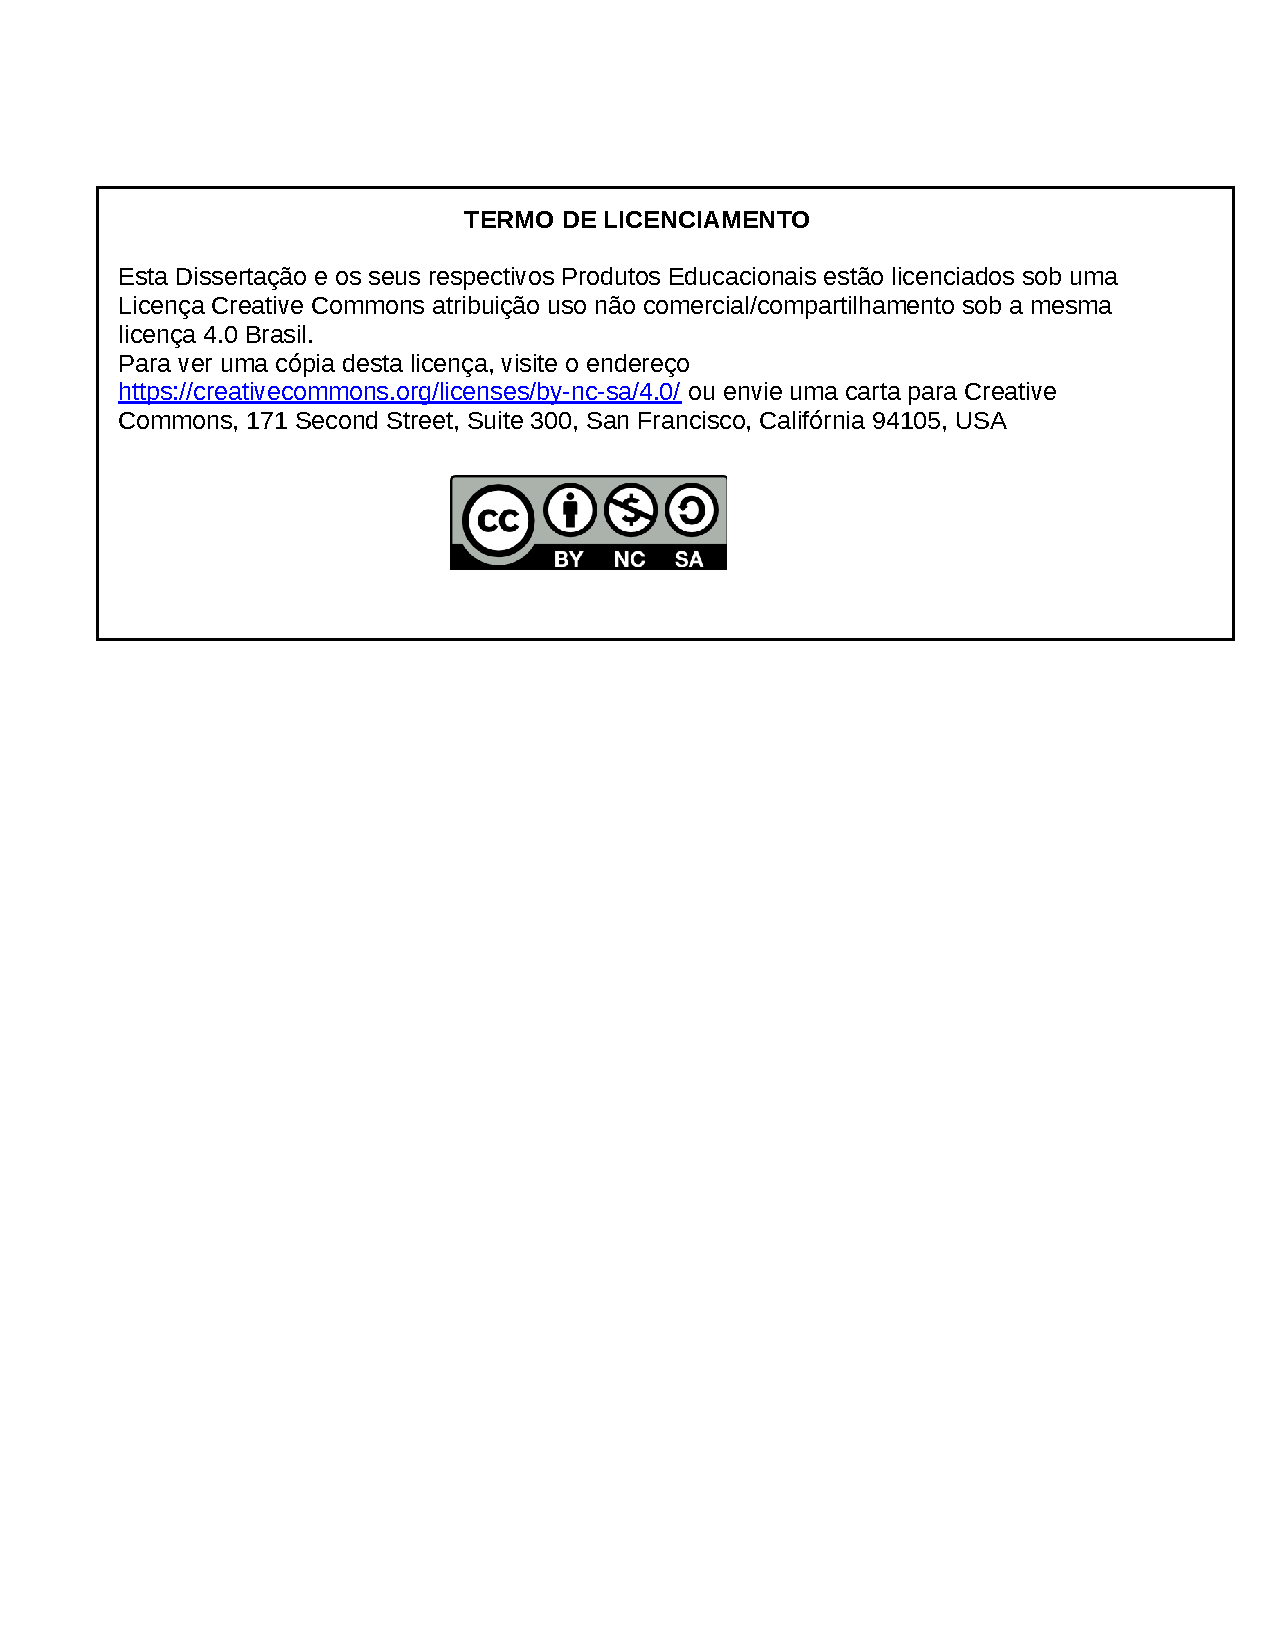
\includepdf{fichacatalografica.pdf}
			 %\end{fichacatalografica}
			 % Se voc\^e optar por elaborar a ficha catalogr\'afica, dever\'a 
			 % incluir uma % antes das 3 linhas acima e tirar a % antes
			 % do comando %% USPSC-fichacatalografica.tex
% ---
% Inserir a ficha bibliografica
% ---
% Isto \'e um exemplo de Ficha Catalogr\'afica, ou ``Dados internacionais de
% cataloga\c{c}\~ao-na-publica\c{c}\~ao''. Voc\^e pode utilizar este modelo como refer\^encia. 
% Por\'em, provavelmente a biblioteca da sua universidade lhe fornecer\'a um PDF
% com a ficha catalogr\'afica definitiva ap\'os a defesa do trabalho. Quando estiver
% com o documento, salve-o como PDF no diret\'orio do seu projeto e substitua todo
% o conte\'udo de implementa\c{c}\~ao deste arquivo pelo comando abaixo:
%
\begin{fichacatalografica}
	\hspace{-1.4cm}
	\imprimirnotaautorizacao \\ \\
	%\sffamily
	\vspace*{\fill}					% Posi\c{c}\~ao vertical
\begin{center}					% Minipage Centralizado
  \imprimirnotabib \\
  \begin{table}[htb]
	\scriptsize
	\centering	
	\begin{tabular}{|p{0.9cm} p{8.7cm}|}
		\hline
	      & \\
		  &	  \imprimirautorficha     \\
		
		 \imprimircutter & 
							\hspace{0.4cm}\imprimirtitulo~  / ~\imprimirautor~ ;  ~\imprimirorientadorcorpoficha. -- 	\imprimirlocal, \imprimirdata.   \\
		
		  &  % Para incluir nota referente \`a vers\~ao corrigida no corpo da ficha,
			  % incluir % no in\'{\i}cio da linha acima e tirar a % do in\'{\i}cio da linha abaixo
			  %	\hspace{0.4cm} \imprimirtitulo~  / ~\imprimirautor~ ; ~\imprimirorientadorcorpoficha~- ~\imprimirnotafolharosto. -- \imprimirlocal, \imprimirdata.  \\
		
			\hspace{0.4cm}\pageref{LastPage} p. : il. (algumas color.) ; 30 cm.\\ 
		  & \\
		  & 
		    \hspace{0.4cm}\imprimirnotaficha ~--~ 
						  \imprimirunidademin, 
						  \imprimiruniversidademin, 
		                  \imprimirdata. \\ 
		  & \\                 
		   % Para incluir nota referente \`a vers\~ao corrigida em notas,
		    % incluir uma % no in\'{\i}cio da linha acima e	
		    % tirar a % do in\'{\i}cio da linha abaixo
		    % & \hspace{0.4cm}\imprimirnotafolharosto \\ 
		  & \\ 
		  & \hspace{0.4cm}1. LaTeX. 2. abnTeX. 3. Classe USPSC. 4. Editora\c{c}\~ao de texto. 5. Normaliza\c{c}\~ao da documenta\c{c}\~ao. 6. Tese. 7. Disserta\c{c}\~ao. 8. Documentos (elabora\c{c}\~ao). 9. Documentos eletr\^onicos. I. \imprimirorientadorficha. 
		   II. T\'{\i}tulo. \\
	
		     %Se houver co-orientador, inclua % antes da linha (antes de II. T\'{\i}tulo.) 
		     %          e tire a % antes do comando abaixo 
		     %III. T\'{\i}tulo. \\   
		  \hline
	\end{tabular}
  \end{table}
\end{center}
\end{fichacatalografica}
% ---


			 %% USPSC-fichacatalografica.tex
% ---
% Inserir a ficha bibliografica
% ---
% Isto \'e um exemplo de Ficha Catalogr\'afica, ou ``Dados internacionais de
% cataloga\c{c}\~ao-na-publica\c{c}\~ao''. Voc\^e pode utilizar este modelo como refer\^encia. 
% Por\'em, provavelmente a biblioteca da sua universidade lhe fornecer\'a um PDF
% com a ficha catalogr\'afica definitiva ap\'os a defesa do trabalho. Quando estiver
% com o documento, salve-o como PDF no diret\'orio do seu projeto e substitua todo
% o conte\'udo de implementa\c{c}\~ao deste arquivo pelo comando abaixo:
%
\begin{fichacatalografica}
	\hspace{-1.4cm}
	\imprimirnotaautorizacao \\ \\
	%\sffamily
	\vspace*{\fill}					% Posi\c{c}\~ao vertical
\begin{center}					% Minipage Centralizado
  \imprimirnotabib \\
  \begin{table}[htb]
	\scriptsize
	\centering	
	\begin{tabular}{|p{0.9cm} p{8.7cm}|}
		\hline
	      & \\
		  &	  \imprimirautorficha     \\
		
		 \imprimircutter & 
							\hspace{0.4cm}\imprimirtitulo~  / ~\imprimirautor~ ;  ~\imprimirorientadorcorpoficha. -- 	\imprimirlocal, \imprimirdata.   \\
		
		  &  % Para incluir nota referente \`a vers\~ao corrigida no corpo da ficha,
			  % incluir % no in\'{\i}cio da linha acima e tirar a % do in\'{\i}cio da linha abaixo
			  %	\hspace{0.4cm} \imprimirtitulo~  / ~\imprimirautor~ ; ~\imprimirorientadorcorpoficha~- ~\imprimirnotafolharosto. -- \imprimirlocal, \imprimirdata.  \\
		
			\hspace{0.4cm}\pageref{LastPage} p. : il. (algumas color.) ; 30 cm.\\ 
		  & \\
		  & 
		    \hspace{0.4cm}\imprimirnotaficha ~--~ 
						  \imprimirunidademin, 
						  \imprimiruniversidademin, 
		                  \imprimirdata. \\ 
		  & \\                 
		   % Para incluir nota referente \`a vers\~ao corrigida em notas,
		    % incluir uma % no in\'{\i}cio da linha acima e	
		    % tirar a % do in\'{\i}cio da linha abaixo
		    % & \hspace{0.4cm}\imprimirnotafolharosto \\ 
		  & \\ 
		  & \hspace{0.4cm}1. LaTeX. 2. abnTeX. 3. Classe USPSC. 4. Editora\c{c}\~ao de texto. 5. Normaliza\c{c}\~ao da documenta\c{c}\~ao. 6. Tese. 7. Disserta\c{c}\~ao. 8. Documentos (elabora\c{c}\~ao). 9. Documentos eletr\^onicos. I. \imprimirorientadorficha. 
		   II. T\'{\i}tulo. \\
	
		     %Se houver co-orientador, inclua % antes da linha (antes de II. T\'{\i}tulo.) 
		     %          e tire a % antes do comando abaixo 
		     %III. T\'{\i}tulo. \\   
		  \hline
	\end{tabular}
  \end{table}
\end{center}
\end{fichacatalografica}
% ---


			 % As informa\c{c}\~oes que comp\~oem a ficha catalogr\'afica est\~ao 
			 % definidas no arquivo USPSC-pre-textual-UUUU.tex
			 % ---
			 \end{verbatim} 
			 				
\'E poss\'{\i}vel incluir ou n\~ao o C\'odigo Cutter na ficha catalogr\'afica, conforme a seguinte orienta\c{c}\~ao nos respectivos arquivos pr\'e-textuais:

\begin{verbatim}
\cutter{S856m}
% Para gerar a ficha catalogr\'afica sem o C\'odigo Cutter, basta 
% incluir uma % na linha acima e tirar a % da linha abaixo
%\cutter{ } 
\end{verbatim} 

Atrav\'es do arquivo fichacatalografica.tex \'e poss\'{\i}vel elaborar a ficha catalogr\'afica em \LaTeX\ . Caso o trabalho possua co-orientador ser\'a necess\'ario seguir as orienta\c{c}\~oes contidas tamb\'em no arquivo com os elementos pr\'e-textuais.	 


\section{Resultados de comandos}\label{sec-divisoes}

O conte\'udo desta se\c{c}\~ao foi baseado no item \textbf{1 Resultados de comandos} do \textbf{Modelo can\^onico de trabalho acad\^emico com abnTEX2} \cite{equipeabntex2}.

% ---
\subsection{Codifica\c{c}\~ao dos arquivos: UTF8}
% ---

A codifica\c{c}\~ao \texttt{UTF8} deve ser utilizada para todos os arquivos do \abnTeX\ . Utilize a mesma codifica\c{c}\~ao nos documentos que escrever, incluindo nos arquivos de bases bibliogr\'aficas |.bib|. Para tanto, tanto o arquivo USPSC-modelo.tex  quanto o USPSC-TCC-modelo.tex devem conter o seguinte pacote:

\begin{verbatim}
\usepackage[utf8]{inputenc}	 % Codificacao do documento (convers\~ao
                               autom\'atica dos acentos)
\end{verbatim}

% ---
\subsection{Diferentes idiomas e hifeniza\c{c}\~oes}
\label{sec-hifenizacao}
% ---

Para usar hifeniza\c{c}\~oes de diferentes idiomas, inclua nas op\c{c}\~oes do documento o
nome dos idiomas que o seu texto cont\'em. Os usu\'arios da Classe USPSC devem utilizar:

\begin{verbatim}
\documentclass[
% -- op\c{c}\~oes da classe memoir --
12pt,		% tamanho da fonte
openright,	% cap\'{\i}tulos come\c{c}am em p\'ag \'{\i}mpar (insere p\'agina vazia caso 
preciso)
twoside,  % para impress\~ao em anverso (frente) e verso. Oposto a oneside - 
Nota: utilizar \imprimirfolhaderosto*
%oneside, % para impress\~ao em p\'aginas separadas (somente anverso) -  
Nota: utilizar \imprimirfolhaderosto
% inclua uma % antes do comando twoside e exclua a % antes do oneside 
a4paper,			% tamanho do papel. 
% -- op\c{c}\~oes da classe abntex2 --
chapter=TITLE,		% t\'{\i}tulos de cap\'{\i}tulos convertidos em letras 
mai\'usculas
% -- op\c{c}\~oes do pacote babel --
english,			% idioma adicional para hifeniza\c{c}\~ao
french,				% idioma adicional para hifeniza\c{c}\~ao
spanish,			% idioma adicional para hifeniza\c{c}\~ao
brazil				% o \'ultimo idioma \'e o principal do documento
% {USPSC-classe/USPSC} configura o cabe\c{c}alho contendo apenas o n\'umero 
da p\'agina
]{USPSC-classe/USPSC}
%]{USPSC-classe/USPSC1}
% Inclua % antes de ]{USPSC-classe/USPSC} e retire a % antes 
de %]{USPSC-classe/USPSC1} para utilizar o 
% cabe\c{c}alho diferenciado para as p\'aginas pares e \'{\i}mpares:
%- p\'aginas \'{\i}mpares: cabe\c{c}alho com se\c{c}\~oes ou subse\c{c}\~oes e o n\'umero da p\'agina
%- p\'aginas pares: cabe\c{c}alho com o n\'umero da p\'agina e o t\'{\i}tulo do cap\'{\i}tulo 
% ---
\end{verbatim}

Desta forma o texto dever\'a ser escrito idioma portugu\^es-brasileiro (\texttt{brazil}), podendo ter cita\c{c}\~oes em ingl\^es, franc\^es e espanhol.

O idioma portugu\^es-brasileiro (\texttt{brazil}) \'e inclu\'{\i}do automaticamente pela
classe \textsf{abntex2}. Por\'em, mesmo assim a op\c{c}\~ao \texttt{brazil} deve ser
informada como a \'ultima op\c{c}\~ao da classe para que todos os pacotes reconhe\c{c}am o
idioma. Vale ressaltar que a \'ultima op\c{c}\~ao de idioma \'e a utilizada por padr\~ao no
documento. 

Portanto, para Classe USPSC, caso deseje escrever um texto em ingl\^es que tenha
cita\c{c}\~oes em espanhol, portugu\^es e franc\^es, voc\^e dever\'a usar:

\begin{verbatim}
\documentclass[
% -- op\c{c}\~oes da classe memoir --
12pt,		% tamanho da fonte
openright,	% cap\'{\i}tulos come\c{c}am em p\'ag \'{\i}mpar (insere p\'agina vazia caso 
preciso)
twoside,  % para impress\~ao em anverso (frente) e verso. Oposto a oneside - 
Nota: utilizar \imprimirfolhaderosto*
%oneside, % para impress\~ao em p\'aginas separadas (somente anverso) -  
Nota: utilizar \imprimirfolhaderosto
% inclua uma % antes do comando twoside e exclua a % antes do oneside 
a4paper,			% tamanho do papel. 
% -- op\c{c}\~oes da classe abntex2 --
chapter=TITLE,		% t\'{\i}tulos de cap\'{\i}tulos convertidos em letras 
mai\'usculas
% -- op\c{c}\~oes do pacote babel --
spanish,			% idioma adicional para hifeniza\c{c}\~ao
french,				% idioma adicional para hifeniza\c{c}\~ao
brazil,				% o \'ultimo idioma \'e o principal do documento
english 			% idioma adicional para hifeniza\c{c}\~ao
% {USPSC-classe/USPSC} configura o cabe\c{c}alho contendo apenas o n\'umero 
da p\'agina
]{USPSC-classe/USPSC}
%]{USPSC-classe/USPSC1}
% Inclua % antes de ]{USPSC-classe/USPSC} e retire a % antes 
de %]{USPSC-classe/USPSC1} para utilizar o 
% cabe\c{c}alho diferenciado para as p\'aginas pares e \'{\i}mpares:
%- p\'aginas \'{\i}mpares: cabe\c{c}alho com se\c{c}\~oes ou subse\c{c}\~oes e o n\'umero da p\'agina
%- p\'aginas pares: cabe\c{c}alho com o n\'umero da p\'agina e o t\'{\i}tulo do cap\'{\i}tulo 
% ---
\end{verbatim}

A lista completa de idiomas suportados, bem como outras op\c{c}\~oes de hifeniza\c{c}\~ao,
est\~ao dispon\'{\i}veis em \citeonline[p.~7-8]{babel2011}. \\

Exemplo de hifeniza\c{c}\~ao em ingl\^es\footnote{Extra\'{\i}do de:
	\url{http://en.wikibooks.org/wiki/LaTeX/Internationalization}}:

\begin{otherlanguage*}{english}
	\textit{Text in English language. This environment switches all language-related
		definitions, like the language specific names for figures, tables etc. to the other
		language. The starred version of this environment typesets the main text
		according to the rules of the other language, but keeps the language specific
		string for ancillary things like figures, in the main language of the document.
		The environment hyphenrules switches only the hyphenation patterns used; it can
		also be used to disallow hyphenation by using the language name
		`nohyphenation'.}
\end{otherlanguage*}

Exemplo de hifeniza\c{c}\~ao em franc\^es\footnote{Extra\'{\i}do de:
	\url{http://bigbrowser.blog.lemonde.fr/2013/02/17/tu-ne-tweeteras-point-le-vatican-interdit-aux-cardinaux-de-tweeter-pendant-le-conclave/}}:

\begin{otherlanguage*}{french}
	\textit{Texte en fran\c{c}ais. Pas question que Twitter ne vienne faire une
		concurrence d\'eloyale \`a la traditionnelle fum\'ee blanche qui marque l'\'election
		d'un nouveau pape. Pour \'eviter toute fuite pr\'ecoce, le Vatican a donc pris un
		peu d'avance, et a d\'ej\`a interdit aux cardinaux qui prendront part au vote
		d'utiliser le r\'eseau social, selon Catholic News Service. Une mesure valable
		surtout pour les neuf cardinaux – sur les 117 du conclave – pratiquants très
		actifs de Twitter, qui auront interdiction pendant toute la p\'eriode de se
		connecter \`a leur compte.}
\end{otherlanguage*}

Exemplo de hifeniza\c{c}\~ao em espanhol\footnote{Extra\'{\i}do de:
	\url{http://internacional.elpais.com/internacional/2013/02/17/actualidad/1361102009_913423.html}}:

\foreignlanguage{spanish}{\textit{Decenas de miles de personas ovacionan al pont\'{\i}fice en su
		pen\'ultimo \'angelus dominical, el primero desde que anunciase su renuncia. El Papa se
		centra en la cr\'{\i}tica al materialismo}}.

O idioma geral do texto pode ser alterado como no exemplo seguinte:

\begin{verbatim}
\selectlanguage{english}

\end{verbatim}

Isso altera automaticamente a hifeniza\c{c}\~ao e todos os nomes constantes de
refer\^encias do documento para o idioma ingl\^es. Consulte o manual da classe para obter orienta\c{c}\~oes adicionais sobre internacionaliza\c{c}\~ao de documentos produzidos com \textsf{\abnTeX} \cite{abnetxclasse}.

Se a op\c{c}\~ao de idioma do texto n\~ao for o portugu\^es, \'e necess\'ario observar o descrito em \ref{idioma}.

% ---
\subsection{Enumera\c{c}\~oes}
% ---

\index{al\'{\i}neas}\index{subal\'{\i}neas}\index{incisos}Quando for necess\'ario enumerar
os diversos assuntos de uma se\c{c}\~ao que n\~ao possua t\'{\i}tulo, esta deve ser
subdividida em al\'{\i}neas \cite[4.2]{nbr6024}:

\begin{alineas}

  \item os diversos assuntos que n\~ao possuam t\'{\i}tulo pr\'oprio, dentro de uma mesma
  se\c{c}\~ao, devem ser subdivididos em al\'{\i}neas; 
  
  \item o texto que antecede as al\'{\i}neas termina em dois pontos;
  \item as al\'{\i}neas devem ser indicadas alfabeticamente, em letra min\'uscula
  seguida de par\^entese. Utilizam-se letras dobradas, quando esgotadas as
  letras do alfabeto;

  \item as letras indicativas das al\'{\i}neas devem apresentar recuo em rela\c{c}\~ao \`a
  margem esquerda;

  \item o texto da al\'{\i}nea deve come\c{c}ar por letra min\'uscula e terminar em
  ponto-e-v\'{\i}rgula, exceto a \'ultima al\'{\i}nea que termina em ponto final;

  \item o texto da al\'{\i}nea deve terminar em dois pontos, se houver subal\'{\i}nea;

  \item a segunda e as seguintes linhas do texto da al\'{\i}nea come\c{c}a sob a
  primeira letra do texto da pr\'opria al\'{\i}nea;
  
  \item subal\'{\i}neas \cite{nbr6024} devem ser conforme as al\'{\i}neas a
  seguir:

  \begin{alineas}
     \item as subal\'{\i}neas devem come\c{c}ar por travess\~ao seguido de espa\c{c}o;

     \item as subal\'{\i}neas devem apresentar recuo em rela\c{c}\~ao \`a al\'{\i}nea;

     \item o texto da subal\'{\i}nea deve come\c{c}ar por letra min\'uscula e terminar em
     ponto-e-v\'{\i}rgula. A \'ultima subal\'{\i}nea deve terminar em ponto final, se n\~ao
     houver al\'{\i}nea subsequente;

     \item a segunda e as seguintes linhas do texto da subal\'{\i}nea come\c{c}am sob a
     primeira letra do texto da pr\'opria subal\'{\i}nea.
  \end{alineas}
  
  \item no \abnTeX\ est\~ao dispon\'{\i}veis os ambientes \texttt{incisos} e
  \texttt{subalineas}, que em suma \'e o mesmo que se criar outro n\'{\i}vel de
  \texttt{alineas}, como nos exemplos \`a seguir:
  
  \begin{incisos}
    \item \textit{Um novo inciso em it\'alico};
  \end{incisos}
  
  \item Al\'{\i}nea em \textbf{negrito}:
  
  \begin{subalineas}
    \item \textit{Uma subal\'{\i}nea em it\'alico};
    \item \underline{\textit{Uma subal\'{\i}nea em it\'alico e sublinhado}}; 
  \end{subalineas}
  
  \item \'Ultima al\'{\i}nea com \emph{\^enfase}.
  
\end{alineas}

% ---
\subsection{Espa\c{c}amento entre par\'agrafos e linhas}\label{sec_espacamento}
% ---

\index{espa\c{c}amento!dos par\'agrafos}O tamanho do par\'agrafo, espa\c{c}o entre a margem
e o in\'{\i}cio da frase do par\'agrafo, \'e definido por:

\begin{verbatim}
   \setlength{\parindent}{1.3cm}
\end{verbatim}

\index{espa\c{c}amento!do primeiro par\'agrafo}Por padr\~ao, n\~ao h\'a espa\c{c}amento no
primeiro par\'agrafo de cada in\'{\i}cio de divis\~ao do documento
(\autoref{sec-divisoes-b}). Por\'em, voc\^e pode definir que o primeiro par\'agrafo
tamb\'em seja indentado, como \'e o caso deste documento. Para isso, apenas inclua o
pacote \textsf{indentfirst} no pre\^ambulo do documento:

\begin{verbatim}
   \usepackage{indentfirst} % Indenta o primeiro par\'agrafo de cada se\c{c}\~ao.
\end{verbatim}

\index{espa\c{c}amento!entre os par\'agrafos}O espa\c{c}amento entre um par\'agrafo e outro
pode ser controlado por meio do comando:

\begin{verbatim}
  \setlength{\parskip}{0.2cm}  % tente tamb\'em \onelineskip
\end{verbatim}

\index{espa\c{c}amento!entre as linhas}O controle do espa\c{c}amento entre linhas \'e
definido por:
\begin{verbatim}
  \OnehalfSpacing       % espa\c{c}amento um e meio (padr\~ao); 
  \DoubleSpacing        % espa\c{c}amento duplo
  \SingleSpacing        % espa\c{c}amento simples	
\end{verbatim}

Para isso, tamb\'em est\~ao dispon\'{\i}veis os ambientes:
\begin{verbatim}
  \begin{SingleSpace} ...\end{SingleSpace}
  \begin{Spacing}{hfactori} ... \end{Spacing}
  \begin{OnehalfSpace} ... \end{OnehalfSpace}
  \begin{OnehalfSpace*} ... \end{OnehalfSpace*}
  \begin{DoubleSpace} ... \end{DoubleSpace}
  \begin{DoubleSpace*} ... \end{DoubleSpace*} 
\end{verbatim}

% ---
\subsection{Tabelas e quadros}

As tabelas e os quadros apresentam os dados de modo resumido, oferecendo uma vis\~ao geral do conte\'udo em quest\~ao, visando facilitar a compreens\~ao do fen\^omeno em estudo. A diferen\c{c}a b\'asica entre ambas est\'a relacionada ao conte\'udo e a formata\c{c}\~ao. 

Tabela \'e o conjunto de dados estat\'{\i}sticos, dispostos em determinada ordem de classifica\c{c}\~ao, que expressam as varia\c{c}\~oes qualitativas de um fen\^omeno. Sua finalidade b\'asica \'e resumir ou sintetizar dados \cite{sibi2016}.

A constru\c{c}\~ao de tabelas deve obedecer os crit\'erios estabelecidos pelo Instituto Brasileiro de Geografia e Estat\'{\i}stica (IBGE) e requeridos pelas normas da ABNT para documentos t\'ecnicos e acad\^emicos.

A \autoref{tab-ibge} \'e um exemplo de tabela alinhada que pode ser longa ou curta, conforme padr\~ao do IBGE.

\begin{table}[Htb]
	%\begin{table}[H]
	\IBGEtab{%
		\caption{Frequ\^encia anual por categoria de usu\'arios}%
		\label{tab-ibge}
	}{%
	\begin{tabular}{ccc}
		\toprule
		Categoria de Usu\'arios & Frequ\^encia de Usu\'arios \\
		\midrule \midrule
		Gradua\c{c}\~ao & 72\% \\
		\midrule 
		P\'os-Gradua\c{c}\~ao & 15\% \\
		\midrule 
		Docente & 10\% \\
		\midrule 
		Outras & 3\% \\
		\bottomrule
	\end{tabular}%
}{%
\fonte{Elaborada pelos autores.}%
\nota{Exemplo de uma nota.}%
\nota[Anota\c{c}\~oes]{Uma anota\c{c}\~ao adicional, que pode ser seguida de v\'arias
	outras.}%

}
\end{table}


\begin{table}[H]
	\IBGEtab{%
		\caption{N\'{\i}veis descritivos dos testes de compara\c{c}\~ao de m\'edias entre grupos para profundidade da les\~ao junto \`a restaura\c{c}\~ao}%
		\label{tabela-ibge}
	}{%
	\begin{tabular}{p{5.5cm}|p{5.5cm}}
		\hline
		\textbf{Resultado} & \textbf{N\'{\i}vel Descritivo} \\ 
		\hline 
		CIC < Ariston & < 0,0001  \\
		Ariston < Am & 0,0118  \\
		Am = Helio & 0,4576  \\
		-100 = Helio & 0,3360  \\
		\hline
	\end{tabular}%
}{%
\fonte{\citeonline{sibi2009}}%
}
\end{table} 

Os \textbf{AP\^ENDICES J-K} exemplificam outras formata\c{c}\~oes de tabelas.

A formata\c{c}\~ao do quadro \'e similar \`a tabela, mas deve ter suas laterais fechadas e conter as linhas horizontais.

% o comando \newpage foi utilizado para for\c{c}ar a quebra de p\'agina

\begin{quadro}[Htb]
	\caption{\label{quadro_modelo}N\'{\i}veis de investiga\c{c}\~ao}
	\begin{tabular}{|p{2.6cm}|p{6.0cm}|p{2.25cm}|p{3.40cm}|}
		\hline
		\textbf{N\'{\i}vel de Investiga\c{c}\~ao} & \textbf{Insumos}  & \textbf{Sistemas de Investiga\c{c}\~ao}  & \textbf{Produtos}  \\
		\hline
		Meta-n\'{\i}vel & Filosofia\index{filosofia} da Ci\^encia  & Epistemologia &
		Paradigma  \\
		\hline
		N\'{\i}vel do objeto & Paradigmas do metan\'{\i}vel e evid\^encias do n\'{\i}vel inferior &
		Ci\^encia  & Teorias e modelos \\
		\hline
		N\'{\i}vel inferior & Modelos e m\'etodos do n\'{\i}vel do objeto e problemas do n\'{\i}vel inferior & Pr\'atica & Solu\c{c}\~ao de problemas  \\
		\hline
	\end{tabular}
	\begin{flushleft}
		%\fonte{\citeonline{van1986}}
		Fonte: \citeonline{van1986}
	\end{flushleft}
\end{quadro} 


Os \textbf{AP\^ENDICES B-I} apresentam exemplos de quadros.

% ---
\subsection{Figuras}\label{sec_figuras}
% ---
\index{figuras}Figuras podem ser criadas diretamente em \LaTeX,
como o exemplo da \autoref{fig_circulo}. \\ 

\begin{figure}[Htb]
	\caption{\label{fig_circulo}A delimita\c{c}\~ao do espa\c{c}o}
	\begin{center}
		\setlength{\unitlength}{9cm}
		\begin{picture}(1,1)
		\put(0,0){\line(0,1){1}}
		\put(0,0){\line(1,0){1}}
		\put(0,0){\line(1,1){1}}
		\put(0,0){\line(1,2){.5}}
		\put(0,0){\line(1,3){.3333}}
		\put(0,0){\line(1,4){.25}}
		\put(0,0){\line(1,5){.2}}
		\put(0,0){\line(1,6){.1667}}
		\put(0,0){\line(2,1){1}}
		\put(0,0){\line(2,3){.6667}}
		\put(0,0){\line(2,5){.4}}
		\put(0,0){\line(3,1){1}}
		\put(0,0){\line(3,2){1}}
		\put(0,0){\line(3,4){.75}}
		\put(0,0){\line(3,5){.6}}
		\put(0,0){\line(4,1){1}}
		\put(0,0){\line(4,3){1}}
		\put(0,0){\line(4,5){.8}}
		\put(0,0){\line(5,1){1}}
		\put(0,0){\line(5,2){1}}
		\put(0,0){\line(5,3){1}}
		\put(0,0){\line(5,4){1}}
		\put(0,0){\line(5,6){.8333}}
		\put(0,0){\line(6,1){1}}
		\put(0,0){\line(6,5){1}}
		\end{picture}
	\end{center}
	\legend{Fonte: \citeonline{equipeabntex2}}
\end{figure}

Outra op\c{c}\~ao \'e incorporar a figura utilizando um arquivo externo, como \'e o caso da \autoref{fig_grafico}. Se a figura que for inclu\'{\i}da se tratar de um diagrama, um gr\'afico ou uma ilustra\c{c}\~ao, que voc\^e mesmo produza, priorize o uso de imagens vetoriais no formato PDF. Com isso, o tamanho do arquivo final do trabalho ser\'a menor e as imagens ter\~ao uma apresenta\c{c}\~ao melhor, principalmente quando impressas, uma vez que imagens vetoriais s\~ao perfeitamente escal\'aveis para qualquer dimens\~ao. Nesse caso, se for utilizar o Microsoft Excel para produzir gr\'aficos, ou o Microsoft Word para ilustra\c{c}\~oes, exporte-os como PDF e os incorpore ao documento conforme o exemplo abaixo. No entanto, para manter a
coer\^encia no uso de software livre (j\'a que voc\^e est\'a usando \LaTeX\  e \abnTeX),
teste a ferramenta \textsf{InkScape}\index{InkScape}
(\url{http://inkscape.org/}). Ela \'e uma excelente op\c{c}\~ao de c\'odigo-livre para
produzir ilustra\c{c}\~oes vetoriais, similar ao CorelDraw\index{CorelDraw} ou ao Adobe
Illustrator\index{Adobe Illustrator}. De todo modo, caso n\~ao seja poss\'{\i}vel
utilizar arquivos de imagens como PDF, utilize qualquer outro formato, como
JPEG, GIF, BMP, etc. Nesse caso, voc\^e pode tentar aprimorar as imagens
incorporadas com o software livre \textsf{Gimp}\index{Gimp}
(\url{http://www.gimp.org/}). Ele \'e uma alternativa livre ao Adobe
Photoshop\index{Adobe Photoshop}. \\

\begin{figure}[H]
	\caption{\label{fig_grafico}Gr\'afico produzido em Excel e salvo como PDF}
	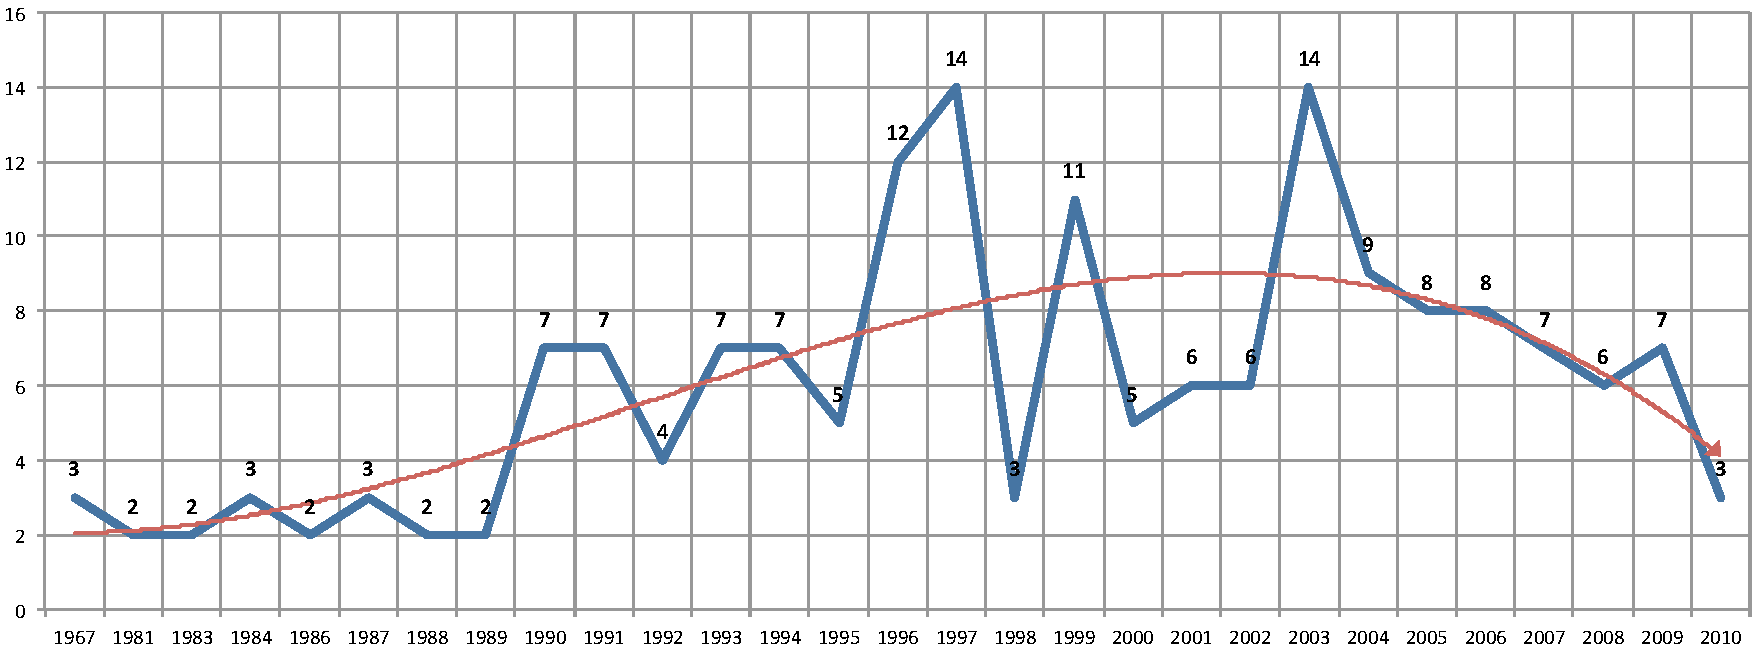
\includegraphics[scale=0.5]{USPSC-img/USPSC-modelo-img-grafico.pdf}
	\begin{flushleft}
		Fonte: \citeonline[p. 24]{araujo2012}
	\end{flushleft}	
\end{figure}

% ---
\subsubsection{Figuras em minipages}
% ---

As ilustra\c{c}\~oes devem sempre ter numera\c{c}\~ao cont\'{\i}nua e \'unica em todo o documento:

% O comando \newpage for\c{c}a a quebra de p\'agina

\begin{citacao}
	Qualquer que seja o tipo de ilustra\c{c}\~ao, sua identifica\c{c}\~ao aparece na parte
	superior, precedida da palavra designativa (desenho, esquema, fluxograma,
	fotografia, gr\'afico, mapa, organograma, planta, quadro, retrato, figura,
	imagem, entre outros), seguida de seu n\'umero de ordem de ocorr\^encia no texto,
	em algarismos ar\'abicos, travess\~ao e do respectivo t\'{\i}tulo. Ap\'os a ilustra\c{c}\~ao, na
	parte inferior, indicar a fonte consultada (elemento obrigat\'orio, mesmo que
	seja produ\c{c}\~ao do pr\'oprio autor), legenda, notas e outras informa\c{c}\~oes
	necess\'arias \`a sua compreens\~ao (se houver). A ilustra\c{c}\~ao deve ser citada no
	texto e inserida o mais pr\'oximo poss\'{\i}vel do trecho a que se
	refere \cite{nbr14724}.
\end{citacao}

\emph{Minipages} s\~ao usadas para inserir textos ou outros elementos em quadros
com tamanhos e posi\c{c}\~oes controladas. Veja o exemplo da
\autoref{fig_minipage_imagem1} e da \autoref{fig_minipage_grafico2}.

\begin{figure}[H]
	\label{teste}
	\centering
	\begin{minipage}{0.4\textwidth}
		\centering
		\caption{Imagem 1 da minipage} \label{fig_minipage_imagem1}
		
\includegraphics[scale=0.9]{USPSC-img/USPSC-modelo-img-marca.pdf}
		\legend{Fonte: \citeonline{equipeabntex2}}
	\end{minipage}
	\hfill
	\begin{minipage}{0.4\textwidth}
		\centering
		\caption{Grafico 2 da minipage} \label{fig_minipage_grafico2}
		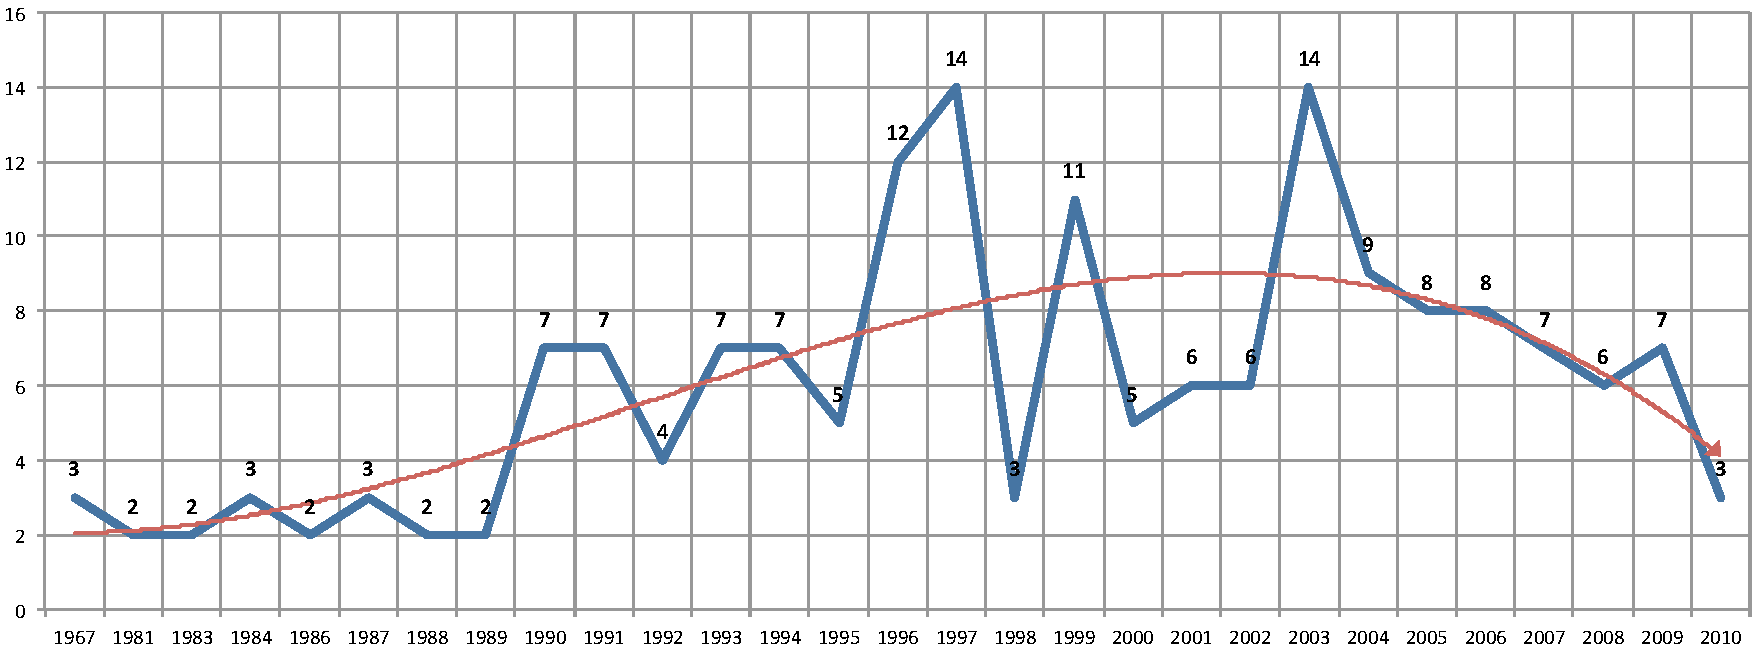
\includegraphics[scale=0.2]{USPSC-img/USPSC-modelo-img-grafico.pdf}
		\legend{Fonte: \citeonline[p. 24]{araujo2012}}
	\end{minipage}
\end{figure}

% ---
\subsection{Express\~oes matem\'aticas}
% ---

\index{express\~oes matem\'aticas}Use o ambiente \texttt{equation} para escrever
express\~oes matem\'aticas numeradas:

\begin{equation}
\forall x \in X, \quad \exists \: y \leq \epsilon
\end{equation}

Escreva express\~oes matem\'aticas entre \$ e \$, como em $ \lim_{x \to \infty}
\exp(-x) = 0 $, para que fiquem na mesma linha.

Tamb\'em \'e poss\'{\i}vel usar colchetes para indicar o in\'{\i}cio de uma express\~ao
matem\'atica que n\~ao \'e numerada.

\[
\left|\sum_{i=1}^n a_ib_i\right|
\le
\left(\sum_{i=1}^n a_i^2\right)^{1/2}
\left(\sum_{i=1}^n b_i^2\right)^{1/2}
\]

Consulte mais informa\c{c}\~oes sobre express\~oes matem\'aticas em
\url{https://github.com/abntex/abntex2/wiki/Referencias}.

\subsection{Estruturas, rea\c{c}\~oes e mecanismos de rea\c{c}\~oes qu\'{\i}micas}\label{Reaquimica}
Para a vers\~ao 3.0 do Pacote USPSC, o Grupo Desenvolvedor optou por utilizar os pacotes \textbf{mychemistry},  \textbf{ChemFig} e o \textbf{TikZ}, que fornecem comandos que permitem compor esquemas complexos de rea\c{c}\~ao qu\'{\i}mica com \LaTeX\ . 

Aqui s\~ao apresentados alguns exemplos, sendo que a maioria foram retirados do manual do pacote \textbf{ChemFig}\cite{ChemFigPac}. 


A f\'ormula estrutural do metano \'e:


\chemfig{C(-[5]H)(-[2]H)(<[:-70]H)(<:[:-20]H)} \\

\begin{verbatim}
\end{verbatim} 

Molecula da Adrenalina \'e:

\chemfig{*6((-HO)-=-(-(<[::60]OH)-[::-60]-[::-60,,,2]
	HN-[::+60]CH_3)=-(-HO)=)} \\

\begin{verbatim}
\end{verbatim}

Com o comando abaixo, o \textbf{ChemFig} possibilita escrever o nome de uma mol\'ecula abaixo dela. 

\begin{verbatim}
\ chemname [hdimi] {\ chemfig {c\'odigo da mol\'ecula}} {hnamei}
\end{verbatim}

Para exemplificar apresentamos uma rea\c{c}\~ao com os nomes das respectivas mol\'eculas:

\schemestart
\chemname{\chemfig{R-C(-[:-30]OH)=[:30]O}}{\'Acido carbox\'{\i}lico}
\+
\chemname{\chemfig{R’OH}}{\'Alcool}
\arrow(.mid east--.mid west)
\chemname{\chemfig{R-C(-[:-30]OR’)=[:30]O}}{\'Ester}
\+
\chemname{\chemfig{H_2O}}{\'Agua}
\schemestop
\chemnameinit{}
 \\

\begin{verbatim}
\end{verbatim}

Mediante a utiliza\c{c}\~ao dos pacotes \textbf{TikZ} e \textbf{ChemFig}, o pacote \textbf{xcolor} \'e carregado possibilitando o uso de cores nos c\'odigos de comandos, conforme exemplos abaixo:

\chemfig{C|{\color{blue}H_3}-C(=[1]O)-[7]O|{\color{red}H}} 

\begin{verbatim}
\end{verbatim}

Para destacar subst\^ancias individualmente ou parte de um esquema, \'e poss\'{\i}vel utilizar recursos tais como os exemplificados a seguir.

\begin{verbatim}
setchemfig{compound style={draw,line width=0.8pt,
semitransparent,text opacity=1,inner sep=8pt,
rounded corners=1mm}}
\schemestart
A\arrow([fill=red]--[fill=blue])[90]
B\arrow(--[fill=gray])
C\arrow(--[fill=green])[-90]
D\arrow(--[draw=none])[-180]
\schemestop
\end{verbatim} 

\begin{verbatim}
\end{verbatim}



\setchemfig{compound style={draw,line width=0.8pt,
		semitransparent,text opacity=1,inner sep=8pt,
		rounded corners=1mm}}
\schemestart
A\arrow([fill=red]--[fill=blue])[90]
B\arrow(--[fill=gray])
C\arrow(--[fill=green])[-90]
D\arrow(--[draw=none])[-180]
\schemestop

\begin{verbatim}
\end{verbatim} 

Mais um exemplo de utiliza\c{c}\~ao dos recursos do pacote TikZ \'e o desenho de duas linhas e um ponto de interse\c{c}\~ao. O comando \verb+ \draw[blue, thick] + define um elemento gr\'afico cuja cor \'e azul e com um tra\c{c}o grosso. A linha \'e definida por seus dois pontos finais, (-1,2) e (2, -4), unidos por -. O comando \verb+ \filldraw[red] (0,0) circle (2pt) + \\ \verb+node[anchor=west] {Intersection point} + ir\'a desenhar um c\'{\i}rculo preenchido com a cor vermelha, sendo que (0,0) define o ponto central, (2pt) determina o raio e, pr\'oximo ao ponto, um n\'o e uma caixa contendo o texto "ponto de interse\c{c}\~ao", ancorado a oeste do ponto.


\begin{verbatim}
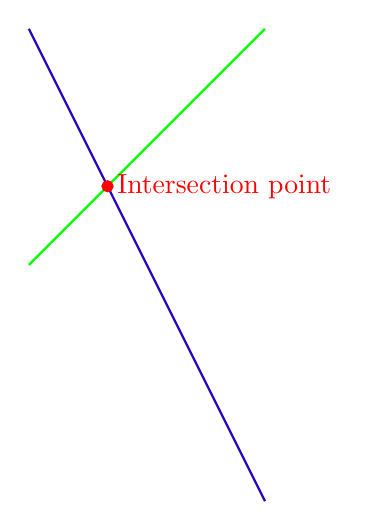
\begin{tikzpicture}
\draw[blue, thick] (-1,2) -- (2,-4);
\draw[green, thick] (-1,-1) -- (2,2);
\filldraw[red] (0,0) circle (2pt) node[anchor=west] {Intersection point};
\end{tikzpicture}
\end{verbatim}

Tais comandos geram os elementos gr\'aficos abaixo:

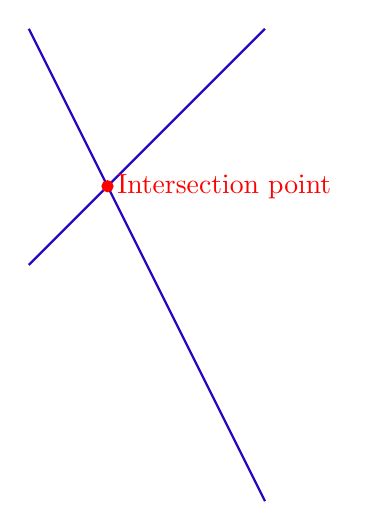
\begin{tikzpicture}
\draw[blue, thick] (-1,2) -- (2,-4);
\draw[blue, thick] (-1,-1) -- (2,2);
\filldraw[red] (0,0) circle (2pt) node[anchor=west] {Intersection point};
\end{tikzpicture}


Para gerar este documento, no pre\^ambulo do arquivo principal (USPSC-modelo.tex e USPSC-TCC-modelo.tex ) foram inclu\'{\i}dos os seguintes comandos:
\begin{verbatim}
\usepackage{float} 				% Fixa tabelas e figuras no local exato
\usepackage{chemfig,chemmacros} % Para escrever rea\c{c}\~oes qu\'{\i}micas
\usepackage{mychemistry}        % Para escrever rea\c{c}\~oes qu\'{\i}micas
\usepackage{tikz}               % Para escrever rea\c{c}\~oes qu\'{\i}micas e outros
\usetikzlibrary{arrows, babel}	% Para escrever rea\c{c}\~oes qu\'{\i}micas e outros
\end{verbatim}

Para informa\c{c}\~oes complementares e recursos adicionais, consulte os manuais dos pacotes utilizados:  \textbf{mychemistry}\cite{mychemistryPac}, \textbf{ChemFig}\cite{ChemFigPac}, \textbf{etoolbox}\cite{etoolboxPack}, \textbf{float}\cite{floatPac}, \textbf{xkeyval}\cite{xkeyvalPac}, \textbf{chemmacros}\cite{chemmacrosPac}, \textbf{TikZ e PGF}\cite{TikZPac} ou de outros necess\'arios para o seu documento.


% ---
\subsection{Inclus\~ao de outros arquivos}\label{sec-include}
% ---

\'E uma boa pr\'atica dividir o seu documento em diversos arquivos, e n\~ao
apenas escrever tudo em um \'unico. Esse recurso foi utilizado neste
documento. Para incluir diferentes arquivos em um arquivo principal,
de modo que cada arquivo inclu\'{\i}do fique em uma p\'agina diferente, utilize o
comando:

\begin{verbatim}
   \include{documento-a-ser-incluido}      % sem a extens\~ao .tex
\end{verbatim}

Para incluir documentos sem quebra de p\'aginas, utilize:

\begin{verbatim}
   \input{documento-a-ser-incluido}      % sem a extens\~ao .tex
\end{verbatim}
% ---
\subsection{\'Indice(s)}
% ---
Elemento  opcional,  que  consiste  em  lista  de  palavras  ou  frases  ordenadas alfabeticamente (autor, t\'{\i}tulo ou assunto) ou sistematicamente (ordena\c{c}\~ao por classes, num\'erica ou cronol\'ogica); localiza e remete para as informa\c{c}\~oes contidas no texto. A pagina\c{c}\~ao deve ser cont\'{\i}nua, dando seguimento ao texto principal \cite{aguia2020}.

Para criar \'{\i}ndice remissivo no \LaTeX\  utilize o pacote makeidx, que deve estar declarado com os demais pacotes. No presente modelo est\'a declarado no arquivo USPSC-modelo.tex, conforme indicado abaixo:

\begin{verbatim}
% ---
% Pacotes b\'asicos - Fundamentais 
% ---
\usepackage[T1]{fontenc}		% Sele\c{c}\~ao de c\'odigos de fonte.
\usepackage[utf8]{inputenc}		% Codifica\c{c}\~ao do documento (convers\~ao 
autom\'atica dos acentos)
\usepackage{lmodern}			% Usa a fonte Latin Modern
% Para utilizar a fonte Times New Roman, inclua uma % no in\'{\i}cio do comando 
acima  "\usepackage{lmodern}"
% Abaixo, tire a % antes do comando  \usepackage{times}
%\usepackage{times}		    	% Usa a fonte Times New Roman	
% Lembre-se de alterar a fonte no comando que imprime o pre\^ambulo no 
arquivo da Classe USPSC.cls				
\usepackage{lastpage}			% Usado pela Ficha catalogr\'afica
\usepackage{indentfirst}		% Indenta o primeiro par\'agrafo de cada se\c{c}\~ao.
\usepackage{color}				% Controle das cores
\usepackage{graphicx}
\usepackage[export]{adjustbox}
			% Inclus\~ao de gr\'aficos
\usepackage{float} 				% Fixa tabelas e figuras no local exato
\usepackage{chemfig,chemmacros} % Para escrever rea\c{c}\~oes qu\'{\i}micas
\usepackage{mychemistry}        % Para escrever rea\c{c}\~oes qu\'{\i}micas
\usepackage{tikz}				% Para escrever rea\c{c}\~oes qu\'{\i}micas e outros
\usetikzlibrary{arrows, babel}	% Para escrever rea\c{c}\~oes qu\'{\i}micas e outros
\usepackage{microtype} 			% para melhorias de justifica\c{c}\~ao
\usepackage{pdfpages}
\usepackage{makeidx}            % para gerar \'{\i}ndice remissivo
% ---
\end{verbatim}

A habilita\c{c}\~ao dos comandos de indexa\c{c}\~ao foi inclu\'{\i}da no arquivo USPSC-modelo.tex da seguinte forma:


\begin{verbatim}
% compila o sum\'ario e \'{\i}ndice
\makeindex
% ---
\end{verbatim}

O presente modelo inclui um exemplo de \'{\i}ndice, gerado a partir da utiliza\c{c}\~ao de comandos similares aos reproduzidos abaixo:

\begin{verbatim}
\index{InkScape}
\index{CorelDraw}
\index{Adobe Illustrator}
\index{Gimp}
\index{Adobe Photoshop}
\index{espa\c{c}amento!do primeiro par\'agrafo}
\index{espa\c{c}amento!dos par\'agrafos}
\index{espa\c{c}amento!entre as linhas}
\index{espa\c{c}amento!entre os par\'agrafos}
\end{verbatim}

Os comandos acima est\~ao no arquivo USPSC-Cap2-Desenvolvimento.tex, em textos na  \autoref{sec_espacamento}  e na  \autoref{sec_figuras}.

Para imprimir o \'{\i}ndice, no final do arquivo USPSC-modelo.tex foi inclu\'{\i}do:

\begin{verbatim}

%---------------------------------------------------------------------
% INDICE REMISSIVO
%--------------------------------------------------------------------
\phantompart
\printindex
%---------------------------------------------------------------------
\end{verbatim}

Para que o \'{\i}ndice seja gerado e inclu\'{\i}do corretamente no texto \'e necess\'ario compil\'a-lo separadamente. No \textbf{TeXstudio 2.9.4}, na barra de menu, selecione \textbf{Tools} e execute \textbf{Index}.


% ---
\subsection{Compilar o documento \LaTeX}
% ---

Geralmente os editores \LaTeX, como o
TeXlipse\footnote{\url{http://texlipse.sourceforge.net/}}, o
Texmaker\footnote{\url{http://www.xm1math.net/texmaker/}}, entre outros,
compilam os documentos automaticamente, de modo que voc\^e n\~ao precisa se
preocupar com isso.

No entanto, voc\^e pode compilar os documentos \LaTeX\ usando os seguintes
comandos, que devem ser digitados no \emph{Prompt de Comandos} do Windows ou no
\emph{Terminal} do Mac ou do Linux:

\begin{verbatim}
   pdflatex ARQUIVO_PRINCIPAL.tex
   bibtex ARQUIVO_PRINCIPAL.aux
   makeindex ARQUIVO_PRINCIPAL.idx 
   makeindex ARQUIVO_PRINCIPAL.nlo -s nomencl.ist -o ARQUIVO_PRINCIPAL.nls
   pdflatex ARQUIVO_PRINCIPAL.tex
   pdflatex ARQUIVO_PRINCIPAL.tex
\end{verbatim}

% ---
\subsection{Remiss\~oes internas}
% ---

Ao nomear a \autoref{tab-ibge} e a \autoref{fig_circulo}, apresentamos um exemplo de remiss\~ao interna, que tamb\'em pode ser feita quando indicamos o
\autoref{cap_exemplos}, que tem o nome \emph{\nameref{cap_exemplos}}. O n\'umero
do cap\'{\i}tulo indicado \'e \ref{cap_exemplos}, que se inicia \`a
\autopageref{cap_exemplos}\footnote{O n\'umero da p\'agina de uma remiss\~ao pode ser
	obtida tamb\'em assim:
	\pageref{cap_exemplos}.}.
Veja a \autoref{sec-divisoes-b} para outros exemplos de remiss\~oes internas entre
se\c{c}\~oes, subse\c{c}\~oes e subsubse\c{c}\~oes.

O c\'odigo usado para produzir o texto desta se\c{c}\~ao \'e:

\begin{verbatim}
Ao nomear a \autoref{tab-nivinv} e a \autoref{fig_circulo}, apresentamos 
um exemplo de remiss\~ao interna, que tamb\'em pode ser feita quando indicamos 
o \autoref{cap_exemplos}, que tem o nome \emph{\nameref{cap_exemplos}}. O
n\'umero do cap\'{\i}tulo indicado \'e \ref{cap_exemplos}, que se inicia \`a 
\autopageref{cap_exemplos}\footnote{O n\'umero da p\'agina de uma remiss\~ao 
pode ser obtida tamb\'em assim: \pageref{cap_exemplos}.}. Veja a 
\autoref{sec-divisoes-b} para outros exemplos de remiss\~oes internas entre 
se\c{c}\~oes, subse\c{c}\~oes e subsubse\c{c}\~oes.
\end{verbatim}

% ---
\section{Divis\~oes do documento}\label{sec-divisoes-b}
Esta se\c{c}\~ao exemplifica o uso de divis\~oes de documentos em conformidade com a ABNT NBR 6024  \cite{nbr6024}.
% ---
% ---
\subsection{Divis\~oes do documento: subse\c{c}\~ao}\label{sec-divisoes-subsection}
% ---

Um exemplo de se\c{c}\~ao \'e a \autoref{sec-divisoes-b}. Esta \'e a \autoref{sec-divisoes-subsection}.

\subsubsection{Divis\~oes do documento: subsubse\c{c}\~ao}\label{sec-divisoes-subsubsection}

Isto \'e uma \texttt{subsubsection} do \LaTeX, mas \'e denominada de ``subse\c{c}\~ao'' porque no portugu\^es n\~ao temos a palavra ``subsubse\c{c}\~ao''.

\subsubsection{Divis\~oes do documento: subsubse\c{c}\~ao}

Isto \'e outra subsubse\c{c}\~ao.

\subsection{Divis\~oes do documento: subse\c{c}\~ao}\label{sec-exemplo-subsec}

Isto \'e uma subse\c{c}\~ao.

\subsubsection{Divis\~oes do documento: subsubse\c{c}\~ao}

Isto \'e mais uma subsubse\c{c}\~ao da \autoref{sec-exemplo-subsec}.


\subsubsubsection{Esta \'e uma subse\c{c}\~ao de quinto
n\'{\i}vel}\label{sec-exemplo-subsubsubsection}

Esta \'e uma se\c{c}\~ao de quinto n\'{\i}vel. Ela \'e produzida com o seguinte comando:

\begin{verbatim}
\subsubsubsection{Esta \'e uma subse\c{c}\~ao de quinto
n\'{\i}vel}\label{sec-exemplo-subsubsubsection}
\end{verbatim}

\subsubsubsection{Esta \'e outra subse\c{c}\~ao de quinto n\'{\i}vel}\label{sec-exemplo-subsubsubsection-outro}

Esta \'e outra se\c{c}\~ao de quinto n\'{\i}vel.


\paragraph{Este \'e um par\'agrafo numerado}\label{sec-exemplo-paragrafo}

Este \'e um exemplo de par\'agrafo nomeado. Ele \'e produzido com o comando de
par\'agrafo:

\begin{verbatim}
\paragraph{Este \'e um par\'agrafo numerado}\label{sec-exemplo-paragrafo}
\end{verbatim}

A numera\c{c}\~ao entre par\'agrafos numerados e subsubsubse\c{c}\~oes s\~ao cont\'{\i}nuas.

\paragraph{Este \'e outro par\'agrafo numerado}\label{sec-exemplo-paragrafo-outro}

Este \'e outro par\'agrafo numerado.

% ---
\subsection{Este \'e um exemplo de nome de subse\c{c}\~ao longa que se aplica a se\c{c}\~oes e demais divis\~oes do documento. Ele deve estar alinhado \`a esquerda e a segunda e demais linhas devem iniciar logo abaixo da primeira palavra da primeira linha} 

Observe que o alinhamento do t\'{\i}tulo obedece esta regra tamb\'em no sum\'ario.
	

% ---
\section{Manual da classe \textsf{\abnTeX}}
% ---

O manual da classe \textsf{\abnTeX} possui uma refer\^encia completa das macros e ambientes dispon\'{\i}veis \cite{abnetxclasse}.

Cont\'em informa\c{c}\~oes adicionais sobre as normas ABNT
observadas pelo \textsf{\abnTeX} e considera\c{c}\~oes sobre eventuais requisitos espec\'{\i}ficos
n\~ao atendidos, como o caso da ABNT NBR 14724 \cite{nbr14724}, que
especifica o espa\c{c}amento entre os cap\'{\i}tulos e o in\'{\i}cio do texto, regra
propositalmente n\~ao atendida pelo presente modelo.

% ---
\section{Precisa de ajuda sobre \textsf{\abnTeX}?}
% ---

Consulte a FAQ com perguntas frequentes e comuns no portal do \textsf{\abnTeX}:
\url{https://github.com/abntex/abntex2/wiki/FAQ}.

Inscreva-se no grupo de usu\'arios \LaTeX:
\url{http://groups.google.com/group/latex-br}, tire suas d\'uvidas e ajude
outros usu\'arios.

Participe tamb\'em do grupo de desenvolvedores do \textsf{\abnTeX}:
\url{http://groups.google.com/group/abntex2} e fa\c{c}a sua contribui\c{c}\~ao \`a
ferramenta.

% ---
\section{Voc\^e pode ajudar?}
% ---

Sua contribui\c{c}\~ao \'e muito importante! Voc\^e pode ajudar na divulga\c{c}\~ao, no
desenvolvimento e de v\'arias outras formas. Veja como contribuir com o \abnTeX\
em \url{https://github.com/abntex/abntex2/wiki/Como-Contribuir}.

% ---
\section{Quer customizar os modelos do \abnTeX\ para sua institui\c{c}\~ao ou
universidade?}
% ---

Veja como customizar o \abnTeX\ em:
\url{https://github.com/abntex/abntex2/wiki/ComoCustomizar}.

% ---
\section{Precisa de ajuda sobre o Pacote USPSC?}
% ---
Consulte a Se\c{c}\~ao de Refer\^encia da Biblioteca de sua institui\c{c}\~ao para obter ajuda sobre o Pacote USPSC.

No Campus USP de S\~ao Carlos, consulte uma das seguintes equipes de refer\^encia:
\begin{verbatim}
EESC - Servi\c{c}o de Biblioteca Prof. Dr. S\'ergio Rodrigues Fontes 
Atendimento ao Usu\'ario
biblioteca.atendimento@eesc.usp.br
(16) 3373-8860

IAU - Biblioteca
Atendimento ao Usu\'ario
bibiau@sc.usp.br
(16) 3373-9282

ICMC - Biblioteca Prof. Achille Bassi
Se\c{c}\~ao de Atendimento ao Usu\'ario
biblio@icmc.usp.br
(16) 3373-8619

IFSC - Servi\c{c}o de Biblioteca e Informa\c{c}\~ao Prof. Bernhard Gross
Se\c{c}\~ao de Atendimento ao Usu\'ario
comut@ifsc.usp.br
(16) 3373-9778

IQSC - Servi\c{c}o de Biblioteca e Informa\c{c}\~ao Prof. Johannes R\'udiger Lechat
Se\c{c}\~ao de Atendimento ao Usu\'ario
bibiqsc@iqsc.usp.br
(16) 3373-9936
\end{verbatim}


O Grupo desenvolvedor do Pacote USPSC esclarece que seu objetivo \'e oferecer um facilitador para os graduandos e p\'os-graduandos, mas n\~ao se compromete a ensinar a Linguagem de Programa\c{c}\~ao \LaTeX .  

% ---
\section{Customize o Pacote USPSC para sua institui\c{c}\~ao}
% ---

Para customizar o \textbf{Modelo para TCC em \LaTeX\ utilizando o Pacote USPSC} e/ou o \textbf{Modelo para teses e disserta\c{c}\~oes em \LaTeX\ utilizando o Pacote USPSC} para outras Unidades da USP e demais institui\c{c}\~oes interessadas em adotar essas normas e padr\~oes, basta criar um arquivo pr\'e-textual contemplando os cursos de gradua\c{c}\~ao e/ou os programas de p\'os-gradua\c{c}\~ao vigentes e incluir a chamada do mesmo em USPSC-unidades.tex.

Para solicitar orienta\c{c}\~oes como proceder, contactar as respons\'aveis pela programa\c{c}\~ao:

\begin{verbatim}
Biblioteca da Prefeitura do Campus USP de S\~ao Carlos - PUSP-SC/USP
Marilza Aparecida Rodrigues Tognetti
Ana Paula Aparecida Calabrez
biblioteca.prefeitura@sc.usp.br
(16) 3373-8316
\end{verbatim}







% ---
% Cap\'{\i}tulo 3 - Cita\c{c}\~oes
% ---
% ---
%% USPSC-Cap3-CitacoesTutorial.tex
% --
% Este capítulo traz os exemplos de citações das "Diretrizes para apresentação de dissertações e teses da USP: documento eletrônico e impresso - Parte I (ABNT)" disponílvel em: http://biblioteca.puspsc.usp.br/pdfFiles_Caderno_Estudos_9_PT_1.pdf


% --- 
\chapter{Citações}
\label{Citações}
% --- 
Citação é a menção no texto de informações extraídas de uma fonte documental que tem o propósito de esclarecer ou fundamentar as ideias do autor. A fonte de onde foi extraída a informação deve ser citada obrigatoriamente, respeitando-se os direitos autorais, conforme ABNT NBR 10520 \cite{nbr10520}.

As citações mencionadas no texto devem, obrigatoriamente, seguir a mesma forma de entrada utilizada nas Referências, no final do trabalho e/ou em Notas de Rodapé.

Todos os documentos relacionados nas Referências devem ser citados no texto, assim como todas as citações do texto devem constar nas Referências. 

Os textos que constam desse manual e os exemplos de citações e referências foram elaborados com base nas \textbf{Diretrizes para apresentação de dissertações e teses da USP}: documento eletrônico e impresso - Parte I (ABNT) \cite{sibi2016}.

Para elaborar as citações utilizando a Classe USPSC é necessário a instalação do pacote: 

\begin{alineas}
	\item \textbf{usepackage[num]abntex2cite:} para gerar citações e referências em estilo numérico;
	\item \textbf{usepackage[alf]abntex2cite:} para gerar citações e referências em estilo alfabético.
\end{alineas}

As explicações para utilização do pacote abntex2cite e exemplos de como elaborar citações e referências de acordo com as normas da ABNT está presente nos manuais: \textbf{O pacote abntex2cite}: estilos bibliográficos compatíveis com a ABNT NBR 6023 \cite{abnetxcite} e  \textbf{O pacote abntex2cite}: tópicos específicos da ABNT NBR 10520:2002 e o estilo bibliográfico alfabético (sistema autor-data) \cite{abnetxcitealf}.

Abaixo seguem alguns exemplos de citações, mas se o exemplo que você precisa não estiver contemplado aqui, acesse o manual \textbf{O pacote abntex2cite} que possui aproximadamente 240 modelos de referências.

Em todo esse documento e especificamente nos exemplos abaixo, foi utilizado o ponto final após o comando \verb+\cite{}+, em conformidade com sistema autor-data. Para o sistema numérico é necessário utilizar o ponto final antes do comando \verb+\cite{}+. 

Alertamos que se este documento for alterado para sistema numérico a pontuação final ficará incorreta. 

\section{Citação direta}

É a transcrição (reprodução integral) de parte da obra consultada, conservando-se a grafia, pontuação, idioma etc.

A reprodução de um texto de \textbf{até três linhas} deve ser incorporada ao parágrafo entre aspas duplas. As aspas simples são utilizadas para indicar citação no interior da citação.

\textbf{Nota:} nas citações diretas é obrigatória a indicação da página.

\textbf{Exemplos: }

\begin{alineas} 
\item 

Segundo \verb+\citeonline[p.~89]{madigan2010}+ “As vesículas de gás são estruturas fusiformes, preenchidas por gás e constituídas de proteínas; elas são ocas, porém rígidas, variando quanto ao comprimento e diâmetro”.

Que corresponde: \\
Segundo \citeonline[p.~89]{madigan2010} “As vesículas de gás são estruturas
fusiformes, preenchidas por gás e constituídas de proteínas; elas são ocas, porém
rígidas, variando quanto ao comprimento e diâmetro”.

\item 

“A comparação é a técnica científica aplicável sempre que houver dois ou
mais termos com as mesmas propriedades gerais ou características particulares”  \verb+\cite[p.~32]{cervo2007}.+

Que corresponde: \\
“A comparação é a técnica científica aplicável sempre que houver dois ou
mais termos com as mesmas propriedades gerais ou características particulares” \cite[p.~32]{cervo2007}.

\end{alineas}

As transcrições com \textbf{mais de três linhas} devem figurar abaixo do texto, com recuo de 4 cm da margem esquerda, com letra menor que a do texto utilizado e sem aspas. 

Utilize o ambiente citação para incluir citações diretas com mais de três linhas.

Use o ambiente assim: \\

\verb+\begin{citação}+

Texto texto texto texto texto texto texto texto texto.

\verb+\end{citação}+

O ambiente citação pode receber como parâmetro opcional um nome de idioma previamente carregado nas opções da classe. Nesse caso, o texto da citação é automaticamente escrito em itálico e a hifenização é ajustada para o idioma selecionado na opção do ambiente.\\
  Por exemplo:
 
\verb+\begin{citacao}[english]+
 
 Text in English language in italic with correct hyphenation.
 
\verb+\end{citacao}+
 
Tem como resultado:
\begin{citacao}[english]
Text in English language in italic with correct hyphenation. \\
\end{citacao}

\textbf{Exemplos:} 

\begin{alineas} 

\item 
De acordo com \verb+\citeonline[p.~35]{cervo2007}+

\verb+\begin{citacao}+

A análise e a síntese racionais só podem ser feitas mentalmente. Empregam-se principalmente na filosofia e na matemática. A análise é uma espécie de indução; parte-se do particular, do complexo, para o princípio geral e mais simples. A síntese é uma espécie de dedução; vai do mais simples ao mais complexo.

\verb+\end{citacao}+

Que corresponde: 

De acordo com \citeonline[p.~35]{cervo2007}

\begin{citacao}
A análise e a síntese racionais só podem ser feitas mentalmente. Empregam-se principalmente na filosofia e na matemática. A análise é uma espécie de indução; parte-se do particular, do complexo, para o princípio geral e mais simples. A síntese é uma espécie de dedução; vai do mais simples ao mais complexo.
\end{citacao}

\item
De acordo com \verb+\citeonline[p.~S4]{Hood1999}+

\verb+\begin{citacao}[english]+

Text in English. Text in English. Text in English. Text in
English. Text in English. Text in English. Text in English. 
Text in English. Text in English. Text in English. Text in
English. Text in English.

\verb+\end{citacao}+

Que corresponde: \\

 De acordo com \citeonline[p.~S4]{Hood1999}
\begin{citacao}[english]
	Text in English. Text in English. Text in English. Text in English. Text in English. Text in English. Text in English. Text in English. Text in English. Text in English Text in English. Text in English.
\end{citacao}

\end{alineas}

\section{Citação indireta}

É o texto criado com base na obra de autor consultado, em que se reproduz o conteúdo e ideias do documento original; dispensa o uso de aspas duplas.

\textbf{Exemplos:}

A hipertemia em bovinos Jersey foi constatada quando a temperatura do ambiente
alcançava 2.5o \verb+\cite{reick1948}+

Que corresponde:

A hipertemia em bovinos Jersey foi constatada quando a temperatura do ambiente
alcançava 2.5o \cite{reick1948}


\section{Citação de citação}

É a citação direta ou indireta de um texto que se refere ao documento original, que não se teve acesso.

Indicar no texto o sobrenome do(s) autor(es) do documento não consultado, seguido da data, da expressão latina apud (citado por) e do sobrenome do(s) autor(es) do documento consultado, data e página. 

Para elaboração de citação de citação são disponibilizados os seguintes comandos: \verb+\apud e \apudonline+.

\textbf{Exemplos:}

\begin{alineas}

\item
Incluir a citação da obra consultada nas referências. 

\citetext{Reis1956}

\item
Mencionar, em nota de rodapé, a referência do trabalho não consultado

\newpage

\textbf{No texto:}

Segundo \apudonline{Segatto1995}{Vianna1986}, “[...] o viés organicista da burocracia estatal e o antiliberalismo da cultura politica de 1937, preservado de modo encapuçado na Carta de 1046”.

-------------------

\textsuperscript{1}\citetext{Vianna1986}

\textbf{Nas Referências:}

\citetext{Segatto1995}

\end{alineas}
\textbf{Nota:}

Este tipo de citação só deve ser utilizada nos casos em que o documento original não foi recuperado (documentos muito antigos, dados insuficientes para a localização do material etc.).

Ressaltamos que os comandos \verb+\apud e \apudonline+ estão em conformidade com ABNT NBR 10520 e para elaborar a citação de citação conforme as Diretrizes da USP, que sugere a inclusão da citação da obra consultada nas referências e mencionar, em nota de rodapé, a referência do trabalho não consultado, é necessário criar a citação conforme abaixo, esse recurso deve ser utilizado para citações com sistema numérico, já que as notas de rodapé estão configuradas com símbolos. 



\begin{alineas}
\item 
\begin{verbatim}
Segundo Vianna\footnote{VIANNA, S. B. \textbf{ A politica econômica 
no segundo Governo Vargas:} 1951-1954. Rio de Janeiro: BNDES, 1986}
(1986, p. 172 apud  \citeauthor{Segatto1995}, 1995, p. 214-215) 
“[...] o viés organicista da burocracia estatal e o antiliberalismo 
da cultura politica de 1937, preservado de modo encapuçado na Carta 
de 1046”.
\end{verbatim}
\end{alineas}


Que Corresponde: \\

Segundo Vianna\footnote{VIANNA, S. B.\textbf{ A politica econômica no segundo Governo Vargas:} 1951-1954. Rio de Janeiro: BNDES, 1986} (1986, p. 172 apud \citeauthor{Segatto1995}, 1995, p. 214-215) “[...] o viés organicista da burocracia estatal e o antiliberalismo da cultura politica de 1937, preservado de modo encapuçado na Carta de 1046”.

\newpage

\textbf{Observação:}

Também é possível escolher dentre os dois comandos: \verb+\footciteref{}+ e o comando \verb+\footnote{\citetext{}}+ para inserir referências em notas de rodapés, mas ao utilizar esses comandos a referência é automaticamente inserida na lista final de referências, constando tanto das notas de rodapés quanto da lista de referências.

\section{Citação de fontes informais}

\textbf{Informação Verbal}

Quando obtidas através de comunicações pessoais, anotações de aulas, trabalhos de eventos não publicados (conferências, palestras, seminários, congressos, simpósios etc.), indicar entre parênteses a expressão (informação verbal), mencionando os dados disponíveis somente em nota de rodapé.

\textbf{Exemplo:}

\begin{alineas}
	\item
	\begin{verbatim}
	Ferreira (2014)\footnote{ Informação fornecida por Ferreira durante 
	o XVIII Seminário Nacional de Bibliotecas Universitárias, Belo 
	Horizonte, 2014.} afirma que as bibliotecas universitárias passam 
	por transformações decorrentes das tecnologias de informação e 
	comunicação (informação verbal).
	\end{verbatim}
\end{alineas}

Que corresponde:

Ferreira (2014)\footnote{ Informação fornecida por Ferreira durante 
o XVIII Seminário Nacional de Bibliotecas Universitárias, Belo Horizonte, 
2014.} afirma que as bibliotecas universitárias passam por transformações decorrentes das tecnologias de informação e comunicação (informação verbal).


\textbf{Informação Pessoal}

Indicar, entre parênteses, a expressão (informação pessoal) para dados obtidos de comunicações pessoais, correspondências pessoais (postal ou \emph{e-mail}), mencionando-se os dados disponíveis em nota de rodapé.

\textbf{Exemplo:}


\begin{alineas}
\item
\begin{verbatim}
Pestana menciona que 20% das bibliotecas [\ldots] (informação 
pessoal).\footnote{ PESTANA, F. O. Bibliotecas de ONGs. 
Mensagem recebida porvmbc@terra.com.br em 13 de abr. 2014.}
\end{verbatim}
\end{alineas}


Que corresponde:

Pestana menciona que 20\% das bibliotecas [\ldots] (informação pessoal).\footnote{ PESTANA, F. O. \textbf{Bibliotecas de ONGs}. Mensagem recebida porvmbc@terra.com.br em 13 de abr. 2014.}\\


\textbf{Em fase de impressão}

Trabalhos em fase de impressão devem ser mencionados nas Referências.

\textbf{Exemplo:}

\begin{alineas}
	\item
PAULA, F. C. E. \textit{et al.} Incinerador de resíduos líquidos e pastosos. \textbf{Revista de
Engenharia e Ciências Aplicadas}, São Paulo, v. 5, 2001. No prelo.
\end{alineas}


\section{Citação de website}

O endereço eletrônico é indicado nas Referências. No texto, a citação é referente ao autor ou ao título do trabalho. 

\textbf{Exemplo:}

\begin{alineas}
\item
\textbf{No texto}
\begin{verbatim}
“[...] a manifestação da CCP deverá ser submetida à deliberação da
CPG.”\cite{USP2013}.
\end{verbatim}
Que corresponde:\\
“[...] a manifestação da CCP deverá ser submetida à deliberação da
CPG.” \cite{USP2013}. \\

\item 
\textbf{Nas referências}\\

UNIVERSIDADE DE SÃO PAULO. Resolução nº 6542, de 18 de abril de 2013.
Baixa o Regimento de Pós-Graduação da Universidade de São Paulo. \textbf{Diário
Oficial [do] Estado de São Paulo}, 20 abr. 2013. Disponível em: http://www.
leginf.usp.br/?resolucao=resolucao-no-6542-de-18-de-abril. Acesso em: 08 jun.
2015.
\end{alineas}

\section{Destaque e supressões no texto}

Utilizar os comandos abaixo durante a redação das citações com destaques e supressões.

\verb+\underline{}+: para grifar.

\verb+\textbf{}+: para colocar em negrito.

\verb+\textit{}+: para colocar em itálico.

\verb+[\ldots]+: para supressões [...]. \\

\textbf{Exemplos:}

\begin{alineas}
\item

\textbf{Destaques}

Usar \underline{grifo} ou \textbf{negrito} ou \textit{itálico} para ênfases ou destaques. Na citação, indicar (grifo nosso ou negrito nosso ou itálico nosso) entre parênteses, logo após a data.

\begin{verbatim}
``Se existe alguém de quem não aceitamos um `não', é porque, na 
verdade,\underline{entregamos o controle de nossa vida a essa 
pessoa}.'' \cite[~p.129, grifo nosso]{Cloud1999} \\
\end{verbatim}	

Que corresponde: \\

``Se existe alguém de quem não aceitamos um `não', é porque, na verdade,
\underline{entregamos o controle de nossa vida a essa pessoa}.'' \cite[~p.129, grifo nosso]{Cloud1999} \\

Usar a expressão “grifo do autor” “negrito do autor” ou "itálico do autor", caso o destaque seja do autor consultado.

\begin{verbatim}
“A palavra \textit{intuição} vem do latim \textit{intuire}, que 
significa \textit{ver por dentro}. O conceito varia conforme a
corrente de pensamento” \cite[~p.47, itálico do autor]{cervo2007}
\end{verbatim}

Que corresponde: \\

“A palavra \textit{intuição} vem do latim \textit{intuire}, que 
significa \textit{ver por dentro}. O conceito varia conforme a
corrente de pensamento” \cite[~p.47, itálico do autor]{cervo2007}\\

\item

\textbf{Supressões}

Indicar as \textbf{supressões} por reticências dentro de colchetes, estejam elas no início, no meio ou no fim do parágrafo e/ou frase.

\begin{verbatim}
Segundo \citeonline[~p.72]{Bottomore1987}  assinala "[\ldots]  
a Sociologia, embora não pretenda ser mais a ciência capaz de 
incluir toda a sociedade [\ldots] pretende ser sinóptica"
\end{verbatim}

Que corresponde:\\

Segundo \citeonline[~p.72]{Bottomore1987}  assinala "[\ldots]  a Sociologia, embora não pretenda ser mais a ciência capaz de incluir toda a sociedade [\ldots] pretende ser sinóptica".\\ 

\item

\textbf{Interpolações}

Indicar as \textbf{interpolações}, comentários, acréscimos e explicações dentro de colchetes, estejam elas no meio ou no fim do parágrafo e/ou frase.

\begin{verbatim}
"não se mova [como se isso fosse possível] faça de conta que 
está morta" \cite[~p.72]{Clarac1985}.
\end{verbatim}

Que corresponde:\\

"não se mova [como se isso fosse possível] faça de conta que 
está morta" \cite[~p.72]{Clarac1985}. \\

\item

\textbf{Tradução feita pelo autor}

Quando a citação incluir uma \textbf{tradução feita pelo autor}, acrescentar a chamada da citação seguida da expressão “tradução nossa”, tudo entre parênteses.

\begin{verbatim}
"A epilepsia pode ocorrer em muitas doenças infecciosas, como 
as causadas por vírus, bactérias e parasitas." \cite[~p.102,
tradução nossa]{Brito2003}.
\end{verbatim}

Que corresponde:\\

"A epilepsia pode ocorrer em muitas doenças infecciosas, como 
as causadas por vírus, bactérias e parasitas." . \cite[~p.102, tradução nossa]{Brito2003}.\\
\end{alineas}

\section{Notas de rodapé}
As notas de rodapé são observações ou esclarecimentos, cujas inclusões no texto são feitas pelo autor do trabalho. Inclui dados obtidos por fontes informais tais como: informação verbal, pessoal, trabalhos em fase de elaboração ou não consultados diretamente.

\newpage

Classificam-se em:\\
\begin{alineas}
\item
\textbf{Notas explicativas} constituem-se em comentários, complementações ou traduções que interromperiam a sequência lógica se colocadas no texto. \cite{Soares2002}

\item
\textbf{Notas de referências} indicam documentos consultados ou remetem a outras partes do texto onde o assunto em questão foi abordado. \\
\end{alineas}

Devem ser digitadas em fontes menores, dentro das margens, ficando separadas do texto por um espaço simples de entrelinhas e por filete de aproximadamente 5 cm, a partir da margem esquerda.

As notas de rodapé podem ser indicadas por numeração consecutiva, com números sobrescritos dentro do capítulo ou da parte (não se inicia a numeração a cada folha).\\

\textbf{Exemplo}

\begin{alineas}

\item

\textbf{No texto:}

Competência: é “uma capacidade específica de executar a ação em um nível de habilidade que seja suficiente para alcançar o efeito desejado” (RHINESMITH\textsuperscript{1}, 1993 apud VERGARA, 2000, p. 38).
Segundo Vergara (2000) mentalidade não é competência. A competência se estabelece a partir de uma mentalidade transformada em comportamento, assim como característica não é competência.
Para Rhinesmith\textsuperscript{2} (1993 apud VERGARA, 2000, p. 38) as competências a seguir complementam as mencionadas anteriormente:

\textbf{Em nota de rodapé:}

---------------------

\textsuperscript{1}RHINESMITH, S. Guia gerencial para globalização. Rio de Janeiro: Berkeley, 1993.

\textsuperscript{2}Ibid, p. 38-39.


\end{alineas}

\textbf{Notas}

Os exemplos de inserção de notas de rodapé já foram expostos nos itens 3.3 e 3.4.

Se a opção for pelo sistema de chamada numérico, a indicação da nota de rodapé deverá ser por símbolos (ex.: asterisco etc.). 
Este modelo está com o sistema numérico para nota de rodapés para mudar para simbólico é necessário ativar o comando \verb+\renewcommand{\thefootnote}{\fnsymbol{footnote}}+

\section{Expressões Latinas}

As expressões latinas podem ser usadas para evitar repetições
constantes de fontes citadas anteriormente. A primeira citação de uma obra
deve apresentar sua referência completa e as subsequentes podem aparecer
sob forma abreviada (Quadro 1).
Não usar destaque tipográfico quando utilizar expressões latinas.
As expressões latinas não devem ser usadas no texto, apenas em nota
de rodapé, exceto a expressão apud.
A presença da referência em nota de rodapé não dispensa sua inclusão
nas Referências, no final do trabalho.

As expressões idem, ibidem, opus citatum, passim, só podem ser usadas na mesma página ou folha da citação a que se referem.

Para não prejudicar a leitura é recomendado evitar o emprego de
expressões latinas.


\section{Apresentação de Autores no Texto}

As citações devem ser indicadas no texto por um dos sistemas de chamada: autor-data ou numérico.

Qualquer que seja o sistema adotado deve ser seguido ao longo de todo o trabalho. 

Para a citação, consideram-se como elementos identificadores: autoria pessoal, institucional ou entrada pela primeira palavra do título em caso de autoria desconhecida e ano da publicação referida.

A forma da entrada do nome do autor pessoal ou institucional na citação deve ser a mesma utilizada nas Referências ou em notas de rodapé.

Para a citação direta é obrigatório incluir o número da página.

Nas citações as chamadas pelo sobrenome do autor, pela instituição responsável ou pelo título incluído na sentença ou entre parênteses devem estar em letras maiúsculas e minúsculas.

\subsection{Alternativas de formatação}
Nesse sistema, a indicação da fonte é feita da seguinte forma:

\begin{alineas}
	\item
	no caso de citação direta, para obras com indicação de autoria ou responsabilidade. Pelo sobrenome de cada autor ou pelo nome da entidade responsável, até o primeiro sinal de pontuação, seguido da data de publicação do documento e da página de citação, separados por vírgula e entre parênteses. Para as citações indiretas o número das páginas é opcional;
	\item
	no caso de citação direta, para obras sem indicação de autoria ou responsabilidade. Pela primeira palavra do título, seguida de reticências, da data de publicação do documento e da(s) página(s) da citação direta, separados por vírgula e entre parênteses. Para as citações indiretas o número das páginas é opcional;
	\item
	se o título iniciar por artigo (definido ou indefinido), ou monossílabo, este deve ser incluído na indicação da fonte.
	
\end{alineas}
	
\section{Exemplos de citações}

Nesta seção são apresentados diversos exemplos de citações diferenciando os elementos identificadores. 

\subsection{Um autor}

Pelo sobrenome\\

[\ldots] duas camadas têm ainda morfologia e funções diferentes \cite{Pereira2013}

ou

\citeonline{Pereira2013} mostrou que duas camadas têm ainda morfologia e funções diferentes.\\


\subsection{Dois autores}

Os sobrenomes dos autores entre parênteses devem ser separados por ponto e vírgula. Quando citados fora de parênteses devem ser separados pela letra “e”\\

[\ldots] \cite{Ramos2014} e de acordo com os resultados obtidos na investigação [\ldots] 

ou 

\citeonline{Ramos2014} obtiveram os resultados de sua investigação [\ldots] \\

\subsection{Três autores}

Os sobrenomes dos autores citados entre parênteses devem ser separados por ponto e vírgula. Quando citados fora de parênteses, os autores devem ser separados por vírgula sendo o último separado pela letra “e”.\\

[\ldots] o acesso ao protótipo \cite{Oliveira2013}

ou

Conforme \citeonline{Oliveira2013} o protótipo [\ldots]\\

\subsection{Quatro ou mais autores}

Indicar o sobrenome do primeiro autor seguido da expressão latina \textit{et al.}\\

[\ldots]  com o grupo de jovens \cite{Sena2012}

ou

\citeonline{Sena2012} pesquisando um grupo de jovens [\ldots]\\

\subsection{Citações consecutivas em Sistema Numérico}

Para agrupar a citação numérica quando for consecutiva:

Adicionar o pacote “cite” junto aos demais pacotes listados inicialmente:

\verb+\usepackage{cite}+ \\

Ao citar a referência:

Para 2 referências consecutivas: 

\verb+\cite{bibtexkey}-\cite{bibtexkey}+ \\

Para 3 ou mais: 

\verb+~\cite{bibtexkey}+ \\

\subsection{Documentos de mesmo autor publicado no mesmo ano}

Quando houver coincidência de trabalhos do mesmo autor publicados
no mesmo ano para identificar o trabalho citado acrescentar letras minúsculas após o ano, sem espaço.\\

[\ldots] \cite{Garcia2013b}   \textbf{\underline{outra obra}}   [\ldots] \cite{Garcia2013a} \\

ou\\

\citeonline{Garcia2013b}  \textbf{\underline{outra obra}}   \citeonline{Garcia2013a}

\subsection{Coincidência de sobrenome e ano}

Quando houver coincidência de sobrenome de autores com trabalhos
publicados no mesmo ano acrescentar as iniciais dos prenomes dos autores
para estabelecer diferenças.\\

[\ldots] (CASTRO FILHO, C., \citeyear{CastroC2012}) \textbf{\underline{outra obra}}   [\ldots] (CASTRO FILHO, M., \citeyear{CastroC2012}) \\

ou\\

Castro Filho, C. (\citeyear{CastroC2012}) \textbf{\underline{outra obra}}    Castro Filho, M. (\citeyear{CastroC2012})

\subsection{Coincidência de sobrenome, inicial do prenome e ano}

Usar os prenomes completos para estabelecer diferenças. \\

 (SOUZA FILHO, Alberto \citeyear{Souza2015}) \textbf{\underline{outra obra}}   [\ldots] (SOUZA FILHO, Amauri, \citeyear{Souza2015}) \\


ou\\


Souza Filho, Alberto (\citeyear{Souza2015}) \textbf{\underline{outra obra}}   [\ldots] Souza Filho, Amauri, (\citeyear{Souza2015}) \\


\subsection{Autoria desconhecida}

Quando o documento não trouxer autoria explícita citar pela primeira palavra do título, seguida de reticências e do ano de publicação.\\

[\ldots] \cite{Controle2015}\\

ou \\

De acordo com a publicação Controle [\ldots] (\citeyear{Controle2015}) estima-se em [\ldots]\\


\subsection{Entidades coletivas}

Citar pela forma em que aparece na referência.\\
\newpage

[\ldots] \cite{Sergipe2010}

ou 

A \citeonline{Sergipe2010} [\ldots] \\


[\ldots] \cite{Food2005}

ou 

A \citeonline{Food2005} [\ldots] \\


\subsection{Patentes}

Citar pela forma em que aparece na referência.\\

[\ldots] \cite{Bagnato2018}

ou 

Para \citeonline{Bagnato2018} [\ldots] \\


[\ldots] \cite{Rocha2017}

ou 

Para \citeonline{Rocha2017} [\ldots] \\


\subsection{Eventos}

Mencionar o nome completo do evento, seguido do ano de publicação.\\

\cite{reuniao1985}\\

ou\\

Os trabalhos apresentados na \citeonline{reuniao1985} [\ldots]\\

\subsection{Vários trabalhos da mesma autoria}

Ao citar vários trabalhos de uma mesma autoria, publicados em anos distintos e mencionados simultaneamente, seguir a ordem cronológica, separando-os com vírgula.\\

[\ldots] (SMITH, \citeyear{Smith1990}, \citeyear{Smith1999}, \citeyear{Smith2002}) \\

ou\\

[\ldots] conforme afirmou Smith (\citeyear{Smith1990}, \citeyear{Smith1999}, \citeyear{Smith2002})\\


\subsection{Vários trabalhos de autorias diferentes}

Ao citar vários trabalhos simultaneamente, de autorias diferentes, indicar
em ordem cronológica. Quando entre parênteses separados por ponto e
vírgula (;) e quando citados fora de parênteses, separados por vírgula (,) e pela
partícula “e”.\\

\citeonline{Ando1990,Ferreira1989,SilvaRibeiro2001}  estudaram [\ldots]\\
	
ou\\

[\ldots] \cite{Ando1990,Ferreira1989,SilvaRibeiro2001}  \\


\section{Comandos em \LaTeX\ para citações}


No texto você deve inserir as citações com os comandos relacionados abaixo:

\begin{alineas}
\item
\begin{verbatim}
\cite
\end{verbatim}

Utilizado para inserir o sobrenome do autor dentro de parênteses seguido da informação do ano.

\textbf{Exemplos} 

\begin{verbatim}
\cite{Paula2001}
\end{verbatim}
\cite{Paula2001}

\begin{verbatim}
\cite{Demakopoulou2000}
\end{verbatim}
\cite{Demakopoulou2000}

\begin{verbatim}
\cite{PhillipiJunior2000}
\end{verbatim}
\cite{PhillipiJunior2000}

\begin{verbatim}
\cite{resprin1997}
\end{verbatim}
\cite{resprin1997}

\begin{verbatim}
\cite{saopaulo1963}
\end{verbatim}
\cite{saopaulo1963}

\begin{verbatim}
\cite{resolucao1991}
\end{verbatim}
\cite{resolucao1991}

\begin{verbatim}
\cite{codigo1985}
\end{verbatim}
\cite{codigo1985}

\begin{verbatim}
\cite{constituicao1988}
\end{verbatim}
\cite{constituicao1988}

\begin{verbatim}
\cite{buscopan2013}
\end{verbatim}
\cite{buscopan2013}

\begin{verbatim}
\cite{Pasquarelli1987}
\end{verbatim}
\cite{Pasquarelli1987}\\

\item
\begin{verbatim}
\citeonline
\end{verbatim}

É utilizado quando você menciona explicitamente o autor da referência na sentença.

\textbf{Exemplos}

\begin{verbatim}
\citeonline{Novak1967}
\end{verbatim}
\citeonline{Novak1967}

\begin{verbatim}
\citeonline{Dood2002}
\end{verbatim}
\citeonline{Dood2002}

\begin{verbatim}
\citeonline{biblioteca1985}
\end{verbatim}
\citeonline{biblioteca1985}

\begin{verbatim}
\citeonline{usp2001}
\end{verbatim}
\citeonline{usp2001}

\begin{verbatim}
\citeonline{educacao2005}
\end{verbatim}
\citeonline{educacao2005}

\begin{verbatim}
\citeonline{brasil1981}
\end{verbatim}
\citeonline{brasil1981}

\begin{verbatim}
\citeonline{brasil1986}
\end{verbatim}
\citeonline{brasil1986}

\begin{verbatim}
\citeonline{Gomes1980}
\end{verbatim}
\citeonline{Gomes1980}\\

\item
\begin{verbatim}
\citeyear
\end{verbatim}

Apenas o \textbf{ano} da obra constará do texto, suprimindo-se os outros dados presentes na citação e os dados bibliográficos continuarão constando da lista de referências. 

\textbf{Exemplos}

\begin{verbatim}
\citeyear{law1967}
\end{verbatim}
\citeyear{law1967}

\begin{verbatim}
\citeyear{Agencia2003}
\end{verbatim}
\citeyear{Agencia2003}

\begin{verbatim}
\citeyear{Dorlands2000}
\end{verbatim}
\citeyear{Dorlands2000}

\begin{verbatim}
\citeyear{abetter2004}
\end{verbatim}
\citeyear{abetter2004}

\begin{verbatim}
\citeyear{abetter2004}
\end{verbatim}
\citeyear{council2001}

\begin{verbatim}
\citeyear{Thome1999}
\end{verbatim}
\citeyear{Thome1999}


\begin{verbatim}
\citeyear{Brennan2006}
\end{verbatim}
\citeyear{Brennan2006}

\begin{verbatim}
\citeyear{microsoft1995}
\end{verbatim}
\citeyear{microsoft1995}\\

\item
\begin{verbatim}
\citeauthor
\end{verbatim}

Apenas o \textbf{sobrenome do autor} da obra constará do texto em letras maiúsculas, suprimindo-se os outros dados presentes na citação e os dados bibliográficos continuarão constando da lista de referências. 

{\tiny {\tiny }}\begin{verbatim}
\citeauthor{Piccini1996} 
\end{verbatim}
\citeauthor{Piccini1996} 

\begin{verbatim}
\citeauthor{Wendel1992}
\end{verbatim}
\citeauthor{Wendel1992}

\begin{verbatim}
\citeauthor{Elewa2006}
\end{verbatim}
\citeauthor{Elewa2006}

\begin{verbatim}
\citeauthor{Hofling1993}
\end{verbatim}
\citeauthor{Hofling1993}

%\begin{verbatim}
%\citeauthor{bule18}
%\end{verbatim}
%\cite{bule18}\\

\item
\begin{verbatim}
\citeauthoronline
\end{verbatim}

Apenas o \textbf{sobrenome do autor} da obra constará do texto, suprimindo-se os outros dados presentes na citação e os dados bibliográficos continuarão constando da lista de referências.

\textbf{Exemplos}

\begin{verbatim}
\citeauthoronline{Fonseca2000}
\end{verbatim}
\citeauthoronline{Fonseca2000}

\begin{verbatim}
\citeauthoronline{bibliotecanacional2000}
\end{verbatim}
\citeauthoronline{bibliotecanacional2000}

\begin{verbatim}
\citeauthoronline{Demakopoulou2000}
\end{verbatim}
\citeauthoronline{Demakopoulou2000}

\begin{verbatim}
\citeauthoronline{GlasscockIII1987}
\end{verbatim}
\citeauthoronline{GlasscockIII1987}

\begin{verbatim}
\citeauthoronline{delvecchio1995}
\end{verbatim}
\citeauthoronline{delvecchio1995}

\begin{verbatim}
\citeauthoronline{brasil1990}
\end{verbatim}
\citeauthoronline{brasil1990}

\begin{verbatim}
\citeauthoronline{Herbrick1989}
\end{verbatim}
\citeauthoronline{Herbrick1989}

\begin{verbatim}
\citeauthoronline{Mostafavi2014}
\end{verbatim}
\citeauthoronline{Mostafavi2014}\\

\item
\begin{verbatim}
\citetext
\end{verbatim}

Imprime o conteúdo da referência de uma citação dentro do texto e também na lista de referências. Ao utilizar a macro  \verb+\citetext+ será transcrito o conteúdo da referência com a formatação padrão do documento, ou seja com espaçamento entre as linhas de 1,5 cm e na lista de referências com espaçamento simples.

\textbf{Exemplos}

\begin{verbatim}
\citetext{Lacasse2005}
\end{verbatim}

\citetext{Lacasse2005} \\

Para alterar o espaçamento entre linhas da referência para simples dentro do documento é necessário inserir o comando de formatação para espaços simples \verb+\SingleSpacing+ conforme abaixo:

\begin{verbatim}
\begin{SingleSpace} 
\citetext{Lacasse2005}
\end{SingleSpace}
\end{verbatim}

\begin{SingleSpace} 
	\citetext{Lacasse2005}
\end{SingleSpace}

Os exemplos abaixo estão formatados com espaçamento simples.

\begin{verbatim}
\begin{SingleSpace} 
\citetext{Palagachev2006}
\end{SingleSpace}
\end{verbatim}

\begin{SingleSpace} 
	\citetext{Palagachev2006}
\end{SingleSpace}

\begin{verbatim}
\begin{SingleSpace} 
\citetext{Zelen2000}
\end{SingleSpace}
\end{verbatim}

\begin{SingleSpace} 
	\citetext{Zelen2000}
\end{SingleSpace}

\begin{verbatim}
\begin{SingleSpace} 
\citetext{Boyd1993}
\end{SingleSpace}
\end{verbatim}

\begin{SingleSpace} 
	\citetext{Boyd1993}
\end{SingleSpace} 

\begin{verbatim}
\begin{SingleSpace} 
\citetext{Cochrane1998}
\end{SingleSpace}
\end{verbatim}

\begin{SingleSpace} 
	\citetext{Cochrane1998}
\end{SingleSpace} 

\begin{verbatim}
\begin{SingleSpace} 
\citetext{Oliveira2006}
\end{SingleSpace}
\end{verbatim}

\begin{SingleSpace} 
	\citetext{Oliveira2006}
\end{SingleSpace}

\begin{verbatim}
\begin{SingleSpace} 
\citetext{Harrison2001}
\end{SingleSpace}
\end{verbatim}

\begin{SingleSpace} 
	\citetext{Harrison2001}
\end{SingleSpace}

\begin{verbatim}
\begin{SingleSpace} 
\citetext{usp2006}
\end{SingleSpace}
\end{verbatim}

\begin{SingleSpace} 
	\citetext{usp2006}
\end{SingleSpace} 

\quad

\item
\begin{verbatim}
\Idem comando específico para mesmo autor
\Ibidem comando específico para mesma obra
\opcit comando específico para obra citada
\passim comando específico para aqui e alí
\loccit comando específico para no lugar citado
\cfcite comando específico para confira
\etseq comando específico para e sequencia 
\end{verbatim} 

As expressões latinas podem ser usadas para evitar repetições constantes de fontes citadas anteriormente. A primeira citação de uma obra deve apresentar sua referência completa e as subsequentes podem aparecer sob forma abreviada. Não usar destaque tipográfico quando utilizar expressões latinas. As expressões latinas não devem ser usadas no texto, apenas em nota de rodapé, exceto apud. A presença da referência em nota de rodapé não dispensa sua inclusão nas Referências, no final do trabalho. As expressões idem, ibidem, opus citatum, passim, loco citato, cf. e et seq. só podem ser usadas na mesma página ou folha da citação a que se referem. Para não prejudicar a leitura é recomendado evitar o emprego de expressões latinas.\\

\textbf{Exemplos}

\begin{verbatim}
\Idem[p.~491]{Abend2002}
\end{verbatim}
\Idem[p.~491]{Abend2002}

\begin{verbatim}
\Idem[p.~15]{tratados1999}
\end{verbatim}
\Idem[p.~15]{tratados1999}

\begin{verbatim}
\Idem[p.~18]{central1998}
\end{verbatim}
\Idem[p.~18]{central1998}

\begin{verbatim}
\Ibidem[p.~1]{Emenda1995}
\end{verbatim}
\Ibidem[p.~1]{Emenda1995}

\begin{verbatim}
\Ibidem[p.~15]{Paciornick1978}
\end{verbatim}
\Ibidem[p.~15]{Paciornick1978}

\begin{verbatim}
\Ibidem[p.~15]{atlas1981}
\end{verbatim}
\Ibidem[p.~35]{atlas1981}

\begin{verbatim}
\opcit[p.~23]{Denver1974}
\end{verbatim}
\opcit[p.~23]{Denver1974}

\begin{verbatim}
\opcit[p.~2]{Almeida1995}
\end{verbatim}
\opcit[p.~2]{Almeida1995}

\begin{verbatim}
\opcit[p.~3]{bionline}
\end{verbatim}
\opcit[p.~3]{bionline}

\begin{verbatim}
\passim{Villa-Lobos1916}
\end{verbatim}
\passim{Villa-Lobos1916}

\begin{verbatim}
\passim{Ramos1999}
\end{verbatim}
\passim{Ramos1999}

\begin{verbatim}
\passim{atlas2001}
\end{verbatim}
\passim{atlas2001}

\begin{verbatim}
\loccit{Wu1999}
\end{verbatim}
\loccit{Wu1999}

\begin{verbatim}
\loccit{Costa2002}
\end{verbatim}
\loccit{Costa2002}

\begin{verbatim}
\loccit{Geografico1986}
\end{verbatim}
\loccit{Geografico1986}

\begin{verbatim}
\cfcite[p.~2]{BRAYNER1994}
\end{verbatim}
\cfcite[p.~2]{BRAYNER1994}

\begin{verbatim}
\cfcite[p.~2]{Sabroza1998}
\end{verbatim}
\cfcite[p.~2]{Sabroza1998}

\begin{verbatim}
\cfcite[p.~46]{Oliva1900}
\end{verbatim}
\cfcite[p.~46]{Oliva1900}

\begin{verbatim}
\etseq[p.~2]{Montgomery1992}
\end{verbatim}
\etseq[p.~2]{Montgomery1992}

\begin{verbatim}
\etseq[p.~2]{Dudek2006}
\end{verbatim}
\etseq[p.~2]{Dudek2006}

\begin{verbatim}
\etseq[p.~2]{brasil1990b}
\end{verbatim}
\etseq[p.~2]{brasil1990b}

\end{alineas}



% ---

% ---
% Cap\'{\i}tulo 4 - Referencias
% ---
% ---
%% USPSC-Cap4-ReferenciasTutorial.tex
% --
% Este cap\'{\i}tulo traz os exemplos de refer\^encias das "Diretrizes para apresenta\c{c}\~ao de disserta\c{c}\~oes e teses da USP: documento eletr\^onico e impresso - Parte I (ABNT)" dispon\'{\i}lvel em: http://biblioteca.puspsc.usp.br/pdfFiles_Caderno_Estudos_9_PT_1.pdf


% --- 
%\chapter{Modelos de re$  $fer\^encias}
\chapter{Modelos de refer\^encias}
\label{Refer\^encias}
% --- 
Elemento obrigat\'orio, que consiste na rela\c{c}\~ao das obras consultadas e citadas no texto, de maneira que permita a identifica\c{c}\~ao individual de cada uma delas. As refer\^encias devem ser organizadas em ordem alfab\'etica, caso as cita\c{c}\~oes no texto obede\c{c}am ao sistema autor-data, ou conforme aparecem no texto, quando utilizado o sistema num\'erico de chamada. \cite{sibi2016}.

Este cap\'{\i}tulo foi elaborado com base nas \textbf{Diretrizes para apresenta\c{c}\~ao de disserta\c{c}\~oes e teses da USP}: documento eletr\^onico e impresso - Parte I (ABNT), 3ª edi\c{c}\~ao de 2016, e todos os exemplos aqui apresentados constam dessas Diretrizes, por\'em em conformidade com ABNT NBR 6023:2018. 

Para organiza\c{c}\~ao, gerenciamento e editora\c{c}\~ao das refer\^encias em BibTeX foi utilizado o software JabRef vers\~ao 2.10.

A ABNT NBR 6023 especifica os elementos a serem inclu\'{\i}dos, fixa sua ordem, orienta a prepara\c{c}\~ao e compila\c{c}\~ao das refer\^encias de materiais utilizados para a produ\c{c}\~ao de documentos e para a inclus\~ao em bibliografias, resumos etc. \cite{nbr6023a}.

Normalmente n\~ao h\'a problemas em usar caracteres acentuados em arquivos bibliogr\'aficos {(*.bib)}. Por\'em, como as regras da ABNT NBR 6023 exigem a convers\~ao do autor ou organiza\c{c}\~ao para letras mai\'usculas, \'e preciso observar o modo como se escrevem os nomes dos autores. No~\autoref{quadro-acentos} voc\^e encontra alguns
exemplos das convers\~oes mais importantes. Preste aten\c{c}\~ao especial para `\c{c}' e `\'{\i}'
que devem estar envoltos em chaves. A regra geral \'e sempre usar a acentua\c{c}\~ao neste modo quando houver convers\~ao para letras mai\'usculas. \cite{abnetxcite} \\

\begin{quadro}[H]
	\caption{\label{quadro-acentos}Convers\~ao de acentua\c{c}\~ao}
		\begin{tabular}{|p{7.5cm}|p{7.5cm}|}
			\hline
			\textbf{Acentos} & \textbf{BibTeX}\\
			\hline
			\`a \'a \~a & \verb+\`a+ \verb+\'a+ \verb+\~a+\\
			\hline
			\'{\i} & \verb+{\'\i}+\\
			\hline
			\c{c} & \verb+{\c c}+\\
			\hline
		\end{tabular}
		\begin{flushleft}
			Fonte: \citeonline{abnetxcite}
		\end{flushleft}	
\end{quadro}


\section{Monografias}

Nesta categoria s\~ao inclu\'{\i}dos livros, folhetos, guias, cat\'alogos, folderes, dicion\'arios e trabalhos acad\^emicos.

Elementos essenciais: autoria, t\'{\i}tulo, edi\c{c}\~ao, local de publica\c{c}\~ao, editora e ano de publica\c{c}\~ao.

Elementos complementares: responsabilidade (tradutor, revisor, ilustrador, entre outros), pagina\c{c}\~ao, s\'erie, notas e ISBN.

O prenome pode estar abreviado ou por extenso, por\'em deve estar padronizado em toda a listagem. \\

\subsection{Monografia no todo}

\begin{tabular}{|l|c|} \hline
SOBRENOME, Prenome(s) do(s) autor(es). \textbf{T\'{\i}tulo da obra}: subt\'{\i}tulo \\ (se houver). Edi\c{c}\~ao (se houver). Local de publica\c{c}\~ao (cidade):	Editora, data \\
de publica\c{c}\~ao.  Pagina\c{c}\~ao. S\'erie. Notas. ISBN.\\\hline
\end{tabular}\\

\subsubsection{Um autor}

\begin{tabular}{|l|c|} \hline
 ESP\'IRITO SANTO, A. \textbf{Ess\^encias de metodologia cient\'{\i}fica}: aplicada \\
 \`a educa\c{c}\~ao. Londrina: Universidade Estadual, 1987. \\\hline
\end{tabular}\\

\textbf{Campos em LATEX:}

\begin{verbatim}
\@Book{EspiritoSanto1987,
Title                    = {Ess\^encias de metodologia cient\'{\i}fica},
Address                  = {Londrina},
Author                   = {Esp{\'\i}rito, Santo, A.},
Publisher                = {Universidade Estadual},
Subtitle                 = {aplicada \`a educa\c{c}\~ao},
Year                     = {1987},
Owner                    = {apcalabrez},
Timestamp                = {2015.09.21}
}
\end{verbatim}

\begin{tabular}{|l|c|} \hline
DE ROSE JUNIOR, D. \textbf{Minibasquetebol na escola}. S\~ao Paulo: \'Icone, \\ 2015. 128 p. \\\hline
\end{tabular}\\

\newpage

\textbf{Campos em LATEX:}

\begin{verbatim}
@Book{DeRose2015,
Title                    = {Minibasquetebol na escola},
Address                  = {S\~ao Paulo},
Author                   = {De, Rose J\'unior, D.},
Pages                    = {128},
Publisher                = {\'Icone},
Year                     = {2015},
Owner                    = {apcalabrez},
Timestamp                = {2015.09.21}
}
\end{verbatim}

\begin{tabular}{|l|c|} \hline
	SMITH, E. B. \textbf{Basic chemical thermodynamics}. 6th ed. London:\\ Imperial College Press, 2014.  \\\hline
\end{tabular}\\

\textbf{Campos em LATEX:}

\begin{verbatim}
@Book{DeRose2015,
Title                    = {Basic chemical thermodynamics},
Address                  = {London},
Edition                  = {6th ed},
Author                   = {SMITH, E. B.},
Publisher                = {Imperial College Press},
Year                     = {2014},
Owner                    = {apcalabrez},
Timestamp                = {2015.09.21}
}
\end{verbatim}

\subsubsection{Dois autores}

\begin{tabular}{|l|c|} \hline
GOMES, C.B.; KEIL, K. \textbf{Brazilian stone meteorites} Albuquerque: \\ Univerity of New Mexico, 1980. \\\hline
\end{tabular}\\

\textbf{Campos em LATEX:}
\begin{verbatim}
@Book{Novak1967,
Title                    = {Brazilian stone meteorites},
Address                  = {Albuquerque},
Author                   = {Gomes, C. B. and Keil, K.},
Publisher                = {University of New Mexico},
Year                     = {1980},
Owner                    = {apcalabrez},
Timestamp                = {2015.09.21}
}
\end{verbatim}

\begin{tabular}{|l|c|} \hline
DIAS, R. B.; COTO, N. P. \textbf{Odontologia do esporte}: hist\'oria e \\ evolu\c{c}\~ao. Rio de Janeiro: MedBook, 2014. \\\hline
\end{tabular}\\

\textbf{Campos em LATEX:}

\begin{verbatim}
@Book{DIAS2014,
Title                    = {Odontologia do esporte},
Subtitle                 = {hist\'oria e evolu\c{c}\~ao},
Address                  = {Rio de Janeiro},
Author                   = {DIAS, R. B.and COTO, N. P.},
Publisher                = {MedBook},
Year                     = {2014},
Owner                    = {apcalabrez},
Timestamp                = {2015.09.21}
}
\end{verbatim}

\subsubsection{Tr\^es autores}

\begin{tabular}{|l|c|} \hline
GIANNINI, S. D.; FORTI, N.; DIAMENT, J. \textbf{Cardiologia preventiva}:\\ preven\c{c}\~ao prim\'aria e secund\'aria. S\~ao Paulo: Atheneu, 2000. \\\hline
\end{tabular}\\
\\
\textbf{Campos em LATEX:}

\begin{verbatim}
@Book{Giannini2000,
Title                    = {Cardiologia preventiva},
Address                  = {S\~ao Paulo},
Author                   = {Giannini, S. D. and Forti, N. and Diament, 
J.},
Publisher                = {Atheneu},
Subtitle                 = {preven\c{c}\~ao prim\'aria e secund\'aria},
Year                     = {2000},
Owner                    = {apcalabrez},
Timestamp                = {2015.09.21}
}
\end{verbatim}

\begin{tabular}{|l|c|} \hline
PAMMI, M.; VALLEJO, J. G.; ABRAMS, S. A. \textbf{Nutrition-infection} \\ \textbf{interactions and impacts on human health}. Hoboken: Taylor and Francis, \\ 2014. \\\hline
\end{tabular}\\

\textbf{Campos em LATEX:}

\begin{verbatim}
@Book{Pammi2000,
Title                    = { Nutrition-infection interactions
and impacts on human health},
Address                  = {Hoboken},
Author                   = {PAMMI, M. and VALLEJO, J. G. and ABRAMS, 
S. A.},
Publisher                = {Taylor and Francis},
Year                     = {2014},
Owner                    = {apcalabrez},
Timestamp                = {2015.09.21}
}
\end{verbatim}

\subsubsection{Quatro autores}

\begin{tabular}{|l|c|} \hline
BAST JUNIOR, C. \textit{et al.} (ed.). \textbf{Cancer medicine}. 
5th ed.	New York: \\ American Cancer Society, 2000. 
\\\hline
\end{tabular}\\

\begin{verbatim}
@Book{bast2000,
Title                    = {Cancer medicine},
Address                  = {New York},
Address                  = {Hamilton},
Edition                  = {5th ed},
Author                   = {Bast Junior, C. et al.},
Publisher                = {American Cancer Society},
Publisher                = {BC Decker},
Year                     = {2000},
Owner                    = {apcalabrez},
Timestamp                = {2015.09.21}
}
\end{verbatim}

\begin{tabular}{|l|c|} \hline
PASQUARELLI, M. L. R. \textit{et al.} \textbf{Avalia\c{c}\~ao do uso de peri\'odicos}. 
S\~ao \\ Paulo: SIBi-USP, 1987. 14 p.\\\hline
\end{tabular}\\

\textbf{Campos em LATEX:}

\begin{verbatim}
@Book{Pasquarelli1987,
Title                    = {Avalia\c{c}\~ao do uso de peri\'odicos},
Address                  = {S\~ao Paulo},
Author                   = {Pasquarelli, M. L. R. and Krzyzanowski,
R. F.; Imperatriz, I. M. M.; Noronha, D. P.; Andrade, E.; Zapparoli,
M. C. M.; Bonesio, M. C. M.; Lobo, M. P.; Almeida, M. S.; Arruda, 
R. M. A.; Plaza, R. T. T.},
Pages                    = {14},
Publisher                = {SIBi-USP},
Year                     = {1987},
Owner                    = {apcalabrez},
Timestamp                = {2015.09.21}
}
\end{verbatim}

\textbf{Nota:} quando houver quatro ou mais autores, conv\'em indicar todos. Permite-se a indica\c{c}\~ao do primeiro autor, seguido da express\~ao \textit{et al.} 

Para desativar a substitui\c{c}\~ao dos autores por ‘et al.’, nas refer\^encias voc\^e deve incluir o pacote com a seguinte op\c{c}\~ao: \verb+\usepackage[alf,abnt-etal-cite=0]{abntex2cite}+

No ~\autoref{quadro-opcoes-etal} est\~ao descritos os comandos dos pacotes de altera\c{c}\~ao da composi\c{c}\~ao dos estilos bibliogr\'aficos para alterar o estilo ‘et al.’.

A obrigatoriedade do \textit{et al.} ser em it\'alico, segundo a ABNT NBR 6023:2018, \'e atendida mediante o par\^ametro \textbf{abnt-etal-text=it} na chamada do pacote \textbf{abntex2cite} no arquivo principal do projeto USPSC-modelo.tex ou USPSC-TCC-modelo.tex. 



\begin{quadro}[H]
	\caption{\label{quadro-opcoes-etal}Op\c{c}\~oes de altera\c{c}\~ao da composi\c{c}\~ao dos estilos bibliogr\'aficos para utiliza\c{c}\~ao da sigla ‘et al.’}
		\begin{tabular}{|p{4.0cm}|p{2.0cm}|p{8.5cm}|}
			\hline
			\textbf{Campo} & \textbf{Op\c{c}\~oes} & \textbf{Descri\c{c}\~ao} \\ 
			\hline
			\emph{abnt-etal-cite} &  & controla como e quando os co-autores s\~ao
			substitu\'{\i}dos por \emph{et al.}  Note que a substitui\c{c}\~ao
			por \emph{et al.} continua ocorrendo \emph{sempre} se os co-autores tiverem sido indicados
			como \texttt{others}.\\
			\hline
			\texttt{abnt-etal-cite=0}&\texttt{0}& n\~ao abrevia a lista de autores.\\
			\hline
			\texttt{abnt-etal-cite=2}& \texttt{2} & abrevia com mais de 2 autores.\\
			\hline
			\texttt{abnt-etal-cite=3}& \texttt{3} & abrevia com mais de 2 autores.\\
			\hline
			$\vdots$ & $\vdots$ & \\
			\hline
			\texttt{abnt-etal-cite=5}& \texttt{5} & abrevia com mais de 5 autores.\\
			\hline
		\end{tabular}
	\begin{flushleft}
		Fonte: \citeonline{abnetxcite}
	\end{flushleft}	
\end{quadro}

Para ver as demais op\c{c}\~oes e o modo de uso dos pacotes de especificidades para formata\c{c}\~ao de refer\^encias veja o documento \textbf{O pacote abntex2cite}. \cite{abnetxcite}.

Sendo assim, para que todos os nomes dos autores constem da refer\^encia basta acrescentar o pacote: 

\verb+\usepackage[alf,abnt-etal-cite=0]{abntex2cite}+

E a refer\^encia ser\'a escrita da seguinte forma: \\

\begin{tabular}{|l|c|} \hline
PASQUARELLI, M. L. R.; KRZYZANOWSKI, R. F.; IMPERATRIZ, I. M.\\
M.; NORONHA, D. P.; ANDRADE, E.; ZAPPAROLI, M. C. M.; BONESIO, \\
M. C. M.; LOBO, M. P.; ALMEIDA, M. S.; ARRUDA, R. M. A.; PLAZA, R. \\ \textbf{Avalia\c{c}\~ao do uso de peri\'odicos}. S\~ao Paulo: SIBi-USP, 1987. 14 p.\\\hline
\end{tabular}\\

\textbf{Campos em LATEX:} permanecer\~ao transcritos da mesma forma.\\

\begin{verbatim}
@Book{Pasquarelli1987,
Title                    = {Avalia\c{c}\~ao do uso de peri\'odicos},
Address                  = {S\~ao Paulo},
Author                   = {Pasquarelli, M. L. R. and Krzyzanowski,
R. F.; Imperatriz, I. M. M.; Noronha, D. P.; Andrade, E.; Zapparoli,
M. C. M.; Bonesio, M. C. M.; Lobo, M. P.; Almeida, M. S.; Arruda, 
R. M. A.; Plaza, R. T. T.},
Pages                    = {14},
Publisher                = {SIBi-USP},
Year                     = {1987},
Owner                    = {apcalabrez},
Timestamp                = {2015.09.21}
}
\end{verbatim}


\subsubsection{Responsabilidade pelo conjunto da obra (editor, organizador,coordenador, compilador entre outros)}

\begin{tabular}{|l|c|} \hline
	DEL VECCHIO, M. (comp.). \textbf{A vista de antejo longa mira}: los \\antejos
	del  Luxottica, as lunetas do Museo Luxottica. Tradu\c{c}\~ao: G. Lizabe \\M. Maglione,  Monique Di Prima. Mil\~ao: Arti Grafiche Salea Luxottica, 1995.  \\\hline
\end{tabular}\\

\textbf{Campos em LATEX:}

\begin{verbatim}
@Book{delvecchio1995,
Title                    = {A Vista de antejo longa mira},
Address                  = {Mil\~ao},
Editor                   = {Del, Vecchio, M},
Editortype               = {comp.},
Furtherresp              = {Tradu\c{c}\~ao: G. Lizabe M. Maglione, Monique 
Di Prima},
Publisher                = {Arti Grafiche Salea Luxottica},
Subtitle                 = {los antejos del Luxottica, as lunetas do 
Museo Luxottica.},
Year                     = {1995},
Owner                    = {apcalabrez},
Timestamp                = {2015.09.21}
}
\end{verbatim}

\begin{tabular}{|l|c|} \hline
	PLOTKIN, S. A.; ORENSTEIN, W. A. (ed.). \textbf{Vaccines}. 3rd ed. Philadelphia: \\ W.B. Saunders, 1999. 1230 p.  \\\hline
\end{tabular}\\

\textbf{Campos em LATEX:}

\begin{verbatim}
@Book{Plotkin1999,
Title                    = {Vaccines.},
Address                  = {Philadelphia},
Editor                   = {Plotkin, S. A. and Orenstein W. A.},
Editortype               = {ed.},
Pages                    = {1230},
Publisher                = {W.B. Saunders},
Year                     = {1999},
Edition                  = {3rd ed},
Owner                    = {apcalabrez},
Timestamp                = {2016.03.31}
}
\end{verbatim}

\begin{tabular}{|l|c|} \hline
	CAVALCANTI, M. G. P. \textit{et al.} (org.). \textbf{Tomografia computadorizada por feixe} \\ \textbf{c\^onico}: interpreta\c{c}\~ao e diagn\'ostico para o cirurgi\~ao-dentista. S\~ao Paulo: Santos, \\ 2010.\\\hline
\end{tabular}\\

\textbf{Campos em LATEX:}

\begin{verbatim}
@Book{Cavalcanti2010,
Title                    = { Tomografia computadorizada 
por feixe c\^onico},
Address                  = {S\~ao Paulo},
Editor                   = {Cavalcanti, M. G. P. and Santos, C. P. and 
Silva, A. M.
and Souza, T. B.},
Editortype               = {org.},
Publisher                = {Santos},
Subtitle                 = {interpreta\c{c}\~ao e diagn\'ostico para o 
cirurgi\~ao-dentista},
Year                     = {2010},
Owner                    = {apcalabrez},
Timestamp                = {2015.09.22}
}
\end{verbatim}

\subsubsection{Outros tipos de responsabilidade (tradutor, prefaciador, ilustrador entre outros)} 


\begin{tabular}{|l|c|} \hline
	BERGSTEIN, R. \textbf{Do tornozelo para baixo:}  a hist\'oria dos
	sapatos e \\ como eles definem as mulheres. Tradu\c{c}\~ao: D\'ebora Guimar\~aes Isidoro.\\ Rio de
	Janeiro: Casa da Palavra, 2013. \\\hline
\end{tabular}\\

\textbf{Campos em LATEX:}

\begin{verbatim}
@Book{Bergstein2013,
Title                    = {Do tornozelo para baixo},
Subtitle                 = {a hist\'oria dos sapatos 
e como eles definem as mulheres}
Author                   = {Bergstein, R.}
Address                  = {Philadelphia},
Editor                   = {Fonseca, R. J.},
Furtherresp              = {Tradu\c{c}\~ao: D\'ebora Guimar\~aes
Isidoro},
Publisher                = {Casa da Palavra},
Year                     = {2013},
Owner                    = {apcalabrez},
Timestamp                = {2015.09.17}
}
\end{verbatim}

\begin{tabular}{|l|c|} \hline
	FONSECA, R. J. (ed.). \textbf{Oral and maxillofacial surgery}. Illustrated by\\
	William M. Winn. Philadelphia: Saunders, 2000. \\\hline
\end{tabular}\\

\textbf{Campos em LATEX:}

\begin{verbatim}
@Book{Fonseca2000,
Title                    = {Oral and maxillofacial surgery},
Address                  = {Philadelphia},
Editor                   = {Fonseca, R. J.},
Editortype               = {ed.},
Furtherresp              = {llustrated by William M. Winn},
Publisher                = {Saunders},
Year                     = {2000},
Owner                    = {apcalabrez},
Timestamp                = {2015.09.17}
}
\end{verbatim}


\subsubsection{Autor entidade (entidades coletivas, governamentais, p\'ublicas, particulares etc.)} 

As obras de responsabilidade de autor entidade (\'org\~aos governamentais, empresas, associa\c{c}\~oes, comiss\~oes, congressos, semin\'arios etc.) t\^em entrada pelo pr\'oprio nome da entidade, por extenso. Seu nome \'e precedido pelo nome do \'org\~ao superior, ou pelo nome da jurisdi\c{c}\~ao geogr\'afica \`a qual pertence. 

No cap\'{\i}tulo \ref{Cita\c{c}\~oes} foram exemplificados algumas cita\c{c}\~oes com  as refer\^encias para entidades coletivas. Conforme exposto anteriormente os arquivos.bib de refer\^encias para entidade coletiva deve conter o comando Org-short que equivale a forma como a refer\^encia ser\'a citada no texto. \\

\begin{tabular}{|l|c|} \hline
	@[unidadefaculdademaiuscula]@
	PAULO.  \textbf{Mapeamento de riscos em encostas e margens de rios}. \\ 
	Bras\'{\i}lia: Minist\'erio das Cidades: IPT, 2007.   \\\hline
\end{tabular}\\

\textbf{Campos em LATEX:}

\begin{verbatim}
@Book{Instituto2007,
Title                    = {Mapeamento de riscos em encostas
e margens de rios},
Address                  = {Bras\'{\i}lia: Minist\'erio das Cidades},
Organization             = {@[unidadefaculdade]@
Tecnol\'ogicas do Estado de S\~ao Paulo},
Publisher                = {IPT},
Year                     = {2007},
Owner                    = {apcalabrez},
Timestamp                = {2015.09.23}
}
\end{verbatim}

\begin{tabular}{|l|c|} \hline
	S\~AO PAULO (Estado). Secretaria da Agricultura. \textbf{O caf\'e}: estat\'{\i}stica de \\produ\c{c}\~ao e commercio 1935-1936. S\~ao Paulo: Typ. Brasil de Rothschild, \\1937. 261 p.  \\\hline
\end{tabular}\\

\textbf{Campos em LATEX:}

\begin{verbatim}
@Book{saopaulo1937,
Title                    = {O caf\'e},
Address                  = {S\~ao Paulo},
Org-short                = {S\~ao Paulo},
Organization             = {S\~ao Paulo {(Estado). Secretaria da 
Agricultura}},
Pages                    = {261},
Publisher                = {Typ. Brasil de Rothschild},
Subtitle                 = {estat\'{\i}stica de produ\c{c}\~ao e commercio 1935-
1936.},
Year                     = {1937},
Owner                    = {apcalabrez},
Timestamp                = {2015.09.23}
}
\end{verbatim}
T

\begin{tabular}{|l|c|} \hline
	U.S. NATIONAL INSTITUTE OF PUBLIC HEALTH. \textbf{Siphonaptera}: \\  a study
	of species infesting wild hares and rabbits of North America,\\ North of Mexico. Washington: GPO, 1988. N\~ao paginado.  \\\hline
\end{tabular}\\

\textbf{Campos em LATEX:}

\begin{verbatim}
@Book{Health1988,
Title                    = {Siphonaptera},
Address                  = {Washington},
Organization             = {U. S. National Institute of Public Health}},
Note                     = {N\~ao paginado},
Publisher                = {GPO},
Subtitle                 = {a study of species infesting 
wild hares and rabbits of North America,},
Year                     = {1988},
Owner                    = {apcalabrez},
Timestamp                = {2015.09.23}
}
\end{verbatim}

Em caso de duplicidade de nomes, deve-se acrescentar entre par\^entese a unidade geogr\'afica que identifica a jurisdi\c{c}\~ao a que pertence. \\


\begin{tabular}{|l|c|} \hline
	BIBLIOTECA NACIONAL (Brasil). \textbf{Movimento de vanguarda na Euro-} \\ \textbf{pa e modernismo brasileiro (1909-1924)}. Rio de Janeiro, 1976.	83 p.   \\\hline
\end{tabular}\\

\textbf{Campos em LATEX:}

\begin{verbatim}
@Book{bibliotecanacional1976,
Title                    = {Movimento de vangarda na Europa e modernismo
brasileiro (1909-1924)},
Address                  = {Rio de Janeiro},
Org-short                = {Biblioteca Nacional {(Brasil)}},
Organization             = {Biblioteca Nacional {(Brasil)}},
Pages                    = {83},
Year                     = {1976},
Owner                    = {apcalabrez},
Timestamp                = {2015.09.23}
}
\end{verbatim}

\begin{tabular}{|l|c|} \hline
	BIBLIOTECA NACIONAL (Portugal). \textbf{O 24 de Julho de 1833 e a} \\ \textbf{guerra civil de 1829-1834}. Lisboa, 1983. 95 p.   \\\hline
\end{tabular}\\

\textbf{Campos em LATEX:}

\begin{verbatim}
@Book{bibliotecanacional1983,
Title                    = {O 24 de Julho de 1833  e a guerra civil de 
1829-1834},
Address                  = {Lisboa},
Org-short                = {Biblioteca Nacional {(Portugal)}},
Organization             = {Biblioteca Nacional {(Portugal)}},
Pages                    = {95},
Year                     = {1983},
Owner                    = {apcalabrez},
Timestamp                = {2015.09.23}
}
\end{verbatim}

\subsubsection{Autoria desconhecida} 

Quando a autoria n\~ao puder ser identificada no documento inicia-se a refer\^encia pelo t\'{\i}tulo.

\begin{tabular}{|l|c|} \hline
	A BETTER investiment climate for everyone. Washington: Oxford University \\ Press, 2004.\\\hline
\end{tabular}\\

\textbf{Campos em LATEX:}

\begin{verbatim}
@Book{abetter2004,
Title                    = {A BETTER investiment climate for everyone},
Address                  = {Washington},
Org-short                = {A Better},
Publisher                = {Oxford University Press},
Year                     = {2004},
Owner                    = {apcalabrez},
Timestamp                = {2015.09.21}
}
\end{verbatim}

\begin{tabular}{|l|c|} \hline
	EDUCA\c{C}\~AO para todos: o imperativo da qualidade. Bras\'{\i}lia, DF: Unesco,\\ 2005.\\\hline
\end{tabular}\\

\textbf{Campos em LATEX:}

\begin{verbatim}
@Book{educacao2005,
Title                    = {Educa{\c c}\~ao para todos},
Address                  = {Bras\'{\i}lia, DF},
Org-short                = {Educa{\c c}\~ao},
Publisher                = {Unesco},
Subtitle                 = {o imperativo da qualidade},
Year                     = {2005},
Owner                    = {apcalabrez},
Timestamp                = {2015.09.21}
}
\end{verbatim}

\subsubsection{Autor(es) com mais de uma obra referenciada } 

Quando se referenciam v\'arias obras do mesmo autor, at\'e a ABNT NBR 6023:2002, era permitido substituir as seguintes por um tra\c{c}o sublinear (equivalente a seis espa\c{c}os) e ponto.

A ABNT NBR 6023:2018 define que o uso do tra\c{c}o sublinear n\~ao \'e mais indicado para representar a mesma autoria do documento anterior na lista de refer\^encia, devendo-se repeti-la quantas vezes forem necess\'ario.

Sendo assim, no Pacote USPSC o par\^ametro \textbf{abnt-repeated-author-omit} est\'a configurado com a op\c{c}\~ao \textbf{no} para exibir os autores em todas as refer\^encias, conforme exemplificado abaixo: 

\verb+\usepackage[alf, abnt-emphasize=bf, abnt-thesis-year=both, + \\ \verb+abnt-repeated-author-omit=no, abnt-last-names=abnt, abnt-etal-cite,+ \\
\verb+abnt-etal-list=3, abnt-etal-text=it, abnt-and-type=e, abnt-doi=doi,+ \\ \verb+abnt-url-package=none, abnt-verbatim-entry=no]{abntex2cite}+ \\

As obras de mesmos autores ser\~ao listadas conforme abaixo: \\

\begin{tabular}{|l|c|} \hline
	PICCINI, A. \textbf{Casa de Babylonia}: estudo da habita\c{c}\~ao rural no interior de \\S\~ao Paulo. S\~ao Paulo: Annablume, 1996. 165 p. \\
	
	PICCINI, A. \textbf{Corti\c{c}os na cidade}: conceito e preconceito na reestrutura\c{c}\~ao do \\centro urbano de  S\~ao Paulo. S\~ao Paulo: Annablume, 1999. 166 p.   \\\hline
\end{tabular}\\

\textbf{Campos em LATEX:}

\begin{verbatim}
@Book{Piccini1996,
Title                    = {Casa de Babylonia},
Address                  = {S\~ao Paulo},
Author                   = {Piccini, A.},
Pages                    = {165},
Publisher                = {Annablume},
Subtitle                 = {estudo da habita\c{c}\~ao rural no interior de 
S\~ao Paulo},
Year                     = {1996},
Owner                    = {apcalabrez},
Timestamp                = {2015.09.23}
}
\end{verbatim}

\begin{verbatim}
Book{Piccini1999,
Title                    = {Corti\c{c}os na cidade},
Address                  = {S\~ao Paulo},
Author                   = {Piccini, A.},
Pages                    = {166},
Publisher                = {Annablume},
Subtitle                 = {conceito e preconceito na reestrutura\c{c}\~ao do 
centro urbano de S\~ao Paulo},
Year                     = {1999},
Owner                    = {apcalabrez},
Timestamp                = {2015.09.21}
}
\end{verbatim}

\subsubsection{Mais de um volume}

\begin{tabular}{|l|c|} \hline
	KUHN, H. A.; LASCH, H. G. \textbf{Avalia\c{c}\~ao cl\'{\i}nica e funcional do doente}. \\S\~ao Paulo:  E.P.U., 1977. 4 v.    \\\hline
\end{tabular}\\

\textbf{Campos em LATEX:}

\begin{verbatim}
@Book{Kuhn1977,
Title                    = {Avalia\c{c}\~ao cl\'{\i}nica e funcional do doente},
Address                  = {S\~ao Paulo},
Author                   = {Kuhn, H. A. and Lasch, H. G.},
Publisher                = {E. P. U.},
Year                     = {1977},
Volume                   = {4},
Owner                    = {apcalabrez},
Timestamp                = {2016.04.11}
}
\end{verbatim}

\begin{tabular}{|l|c|} \hline
	MATSUO, T. \textit{et al.}  \textbf{ Science of the rice plant}. Tokyo: Food and \\ Agriculture Policy Research Center, 1977. 4 v: Genetics. \\\hline
\end{tabular}\\

\textbf{Campos em LATEX:}

\begin{verbatim}
@Book{Matsuo1977,
Title                    = {Science of the rice plant},
Address                  = {Tokyo},
Author                   = {Matsuo, T and Sakomoto, H. A. and Tieko, H. 
G. and Suzuki, A.},
Publisher                = { Food and Agriculture
Policy Research Center,},
Year                     = {1977},
Volume                   = {4: Genetics},
Owner                    = {apcalabrez},
Timestamp                = {2016.04.11}
}
\end{verbatim}

\subsubsection{S\'erie}

\begin{tabular}{|l|c|} \hline
	PHILLIPI J\'UNIOR, A. \textit{et al.} \textbf{Interdisciplinaridade em ci\^encias ambien-}\\ 
	\textbf{tais}. S\~ao Paulo: Signus, 2000. 318 p. (S\'erie textos b\'asicos para a forma\c{c}\~ao \\ambiental, 5). \\\hline
\end{tabular}\\

\textbf{Campos em LATEX:}

\begin{verbatim}
@Book{PhillipiJunior2000,
Title                 = {Interdisciplinaridade em ci\^encias ambientais},
Address               = {S\~ao Paulo},
Author                = {Phillipi, Junior, A. and Medeiros, C. B. and 
Silva, A. M. and Piccini, A.},
Pages                 = {318},
Publisher             = {Signus},
Series                = {S\'erie textos b\'asicos para a forma\c{c}\~ao ambiental, 
5},
Year                  = {2000},
Owner                 = {apcalabrez},
Timestamp             = {2015.09.21}
}
\end{verbatim}

\begin{tabular}{|l|c|} \hline
STEPHENSON, J. B.; KING, M. D. \textbf{ Handbook of neurological}\\ \textbf{investigations in children}. London: Wright, 1989. (Handbooks of \\
investigations in children). \\\hline
\end{tabular}\\

\textbf{Campos em LATEX:}

\begin{verbatim}
@Book{Stephenson1989,
Title                 = {Handbook of neurological
investigations in children},
Address               = {London},
Author                = {Stephenson, J. B and King, M. D.},
Publisher             = {Wright},
Series                = {Handbooks of
investigations in children},
Year                  = {1989},
Owner                 = {apcalabrez},
Timestamp             = {2015.09.21}
}
\end{verbatim}


\subsubsection{Cat\'alogo}

\begin{tabular}{|l|c|} \hline
	BIBLIOTECA NACIONAL (Brasil). \textbf{500 anos de Brasil na Biblioteca }\\ \textbf{Nacional}: cat\'alogo. Rio de Janeiro, 2000. 143 p. Cat\'alogo da exposi\c{c}\~ao em \\comemora\c{c}\~ao aos 500  anos do Brasil e aos 190 anos da Biblioteca Nacional, \\13 de dezembro de 2000 a 20 de abril de 2001.    \\\hline
\end{tabular}\\

\textbf{Campos em LATEX:}

\begin{verbatim}
@Book{bibliotecanacional2000,
Title                    = {500 anos de Brasil na Biblioteca Nacional},
Address                  = {Rio de Janeiro},
Note                     = {Cat\'alogo da exposi\c{c}\~ao em comemora\c{c}\~ao aos 500
anos do Brasil e aos 190 anos da Biblioteca Nacional, 13 de dezembro de
2000 a 20 de abril de 2001},
Org-short                = {Biblioteca Nacional {(Brasil)}},
Organization             = {Biblioteca Nacional {(Brasil)}},
Pages                    = {143},
Subtitle                 = {cat\'alogo},
Year                     = {2000},
Owner                    = {apcalabrez},
Timestamp                = {2015.09.18}
}
\end{verbatim}

\begin{tabular}{|l|c|} \hline
	DEMAKOPOULOU, K. \textit{et al.} \textbf{Gods and heroes of the european}\\ \textbf{bronze age}. London:  Thames and Hudson, 2000. 303 p. Catalog.    \\\hline
\end{tabular}\\

\textbf{Campos em LATEX:}

\begin{verbatim}
@Book{Demakopoulou2000,
Title                    = {Gods and heroes of the european bronze age},
Address                  = {London},
Author                   = {Demakopoulou, K. and Arruda, M. L. and Souza,
L. S. and Saadi, S.},
Note                     = {Catalog},
Pages                    = {303},
Publisher                = {Thames and Hudson},
Year                     = {2000},
Owner                    = {apcalabrez},
Timestamp                = {2015.09.18}
}
\end{verbatim}

\begin{tabular}{|l|c|} \hline
	FARIAS, A. A. C \textbf{Amor = love}: cat\'alogo. S\~ao Paulo: Thomas \\ Cohn, 2001. Cat\'alogo de exposi\c{c}\~ao art\'{\i}stica Beth Moys\'es.    \\\hline
\end{tabular}\\

\textbf{Campos em LATEX:}

\begin{verbatim}
@Book{Farias2001,
Title                    = {Amor = love},
Subtitle                 = {cat\'alogo},
Address                  = {S\~ao Paulo},
Author                   = {Farias, A. A. C.},
Note                     = {Cat\'alogo de exposi\c{c}\~ao
art\'{\i}stica Beth Moys\'es},
Publisher                = {Thomas Cohn},
Year                     = {2001},
Owner                    = {apcalabrez},
Timestamp                = {2015.09.18}
}
\end{verbatim}

\begin{tabular}{|l|c|} \hline
	UNIVERSIDADE DE S\~AO PAULO. Museu de Arqueologia e Etnologia.  \\ \textbf{Brasil 50 mil anos}: uma viagem ao passado pr\'e-colonial, guia tem\'atico \\ para professores: cat\'alogo. [S\~ao Paulo]: Universidade de S\~ao Paulo, Museu \\ de
	Arqueologia e Etnologia, [2001]. 28 p. il. 19 pranchas. Cat\'alogo de \\ exposi\c{c}\~ao.   \\\hline
\end{tabular}\\

\textbf{Campos em LATEX:}

\begin{verbatim}
@Book{USPmuseu2001,
Title                    = {Brasil 50 mil anos},
Address                  = {[S\~ao Paulo]},
Org-short                = {@[universidade]@},
Organization             = {@[universidade]@. {Museu de 
Arqueologia e Etnologia}},
Pages                    = {28},
Publisher                = {Universidade de S\~ao Paulo, Museu de 
Arqueologia e Etnologia},
Subtitle                 = { uma viagem ao passado
pr\'e-colonial, guia tem\'atico para professores: cat\'alogo},
Year                     = {[2001]},
Note                     = { il. 19 pranchas. Cat\'alogo de exposi\c{c}\~ao}
Owner                    = {apcalabrez},
Timestamp                = {2015.09.23}
}
\end{verbatim}

\subsubsection{Relat\'orio e parecer t\'ecnico}

\begin{tabular}{|l|c|} \hline
	CASTRO, M. C. \textit{et al.} \textbf{Coopera\c{c}\~ao t\'ecnica na implementa\c{c}\~ao do
		Pro-}\\\textbf{grama Integrado de Desenvolvimento - Polonordeste}. Bras\'{\i}lia, DF: \\ PNUD: FAO, 1990. 47 p. Relat\'orio da Miss\~ao de Avalia\c{c}\~ao do Projeto \\ BRA/87/037.     \\\hline
\end{tabular}\\

\textbf{Campos em LATEX:}

\begin{verbatim}
@Book{Castro,
Title                    = {Coopera\c{c}\~ao t\'ecnica na implementa\c{c}\~ao do 
Programa Integrado 
de Desenvolvimento - Polonordeste},
Address                  = {Bras\'{\i}lia},
Author                   = {Castro, M. C. and Souza, L. S. and Cardoso, 
R. F and Arruda, M. L.},
Note                     = {Relat\'orio da Miss\~ao de Avalia\c{c}\~ao do 
Projeto BRA/87/037},
Pages                    = {47},
Publisher                = {PNUD: FAO},
Year                     = {1990},

Owner                    = {apcalabrez},
Timestamp                = {2015.09.17}
}
\end{verbatim}

\begin{tabular}{|l|c|} \hline
	COMPANHIA ESTADUAL DE TECNOLOGIA DE SANEAMENTO AMBI-\\ENTAL. \textbf{Bacia hidrogr\'afica do Ribeir\~ao Pinheiros}: relat\'orio t\'ecnico. S\~ao \\Paulo: CETESB, 1994. 39 p.   \\\hline
\end{tabular}\\

\textbf{Campos em LATEX:}

\begin{verbatim}
@Book{Castro,
@Book{CETESB1994,
Title                    = {Bacia hidrogr\'afica do Ribeir\~ao Pinheiros},
Address                  = {S\~ao Paulo},
Organization             = {Companhia Estadual de Tecnologia de 
Saneamento Ambiental},
Pages                    = {39},
Publisher                = {CETESB},
Subtitle                 = {relat\'orio t\'ecnico},
Year                     = {1994},
Owner                    = {apcalabrez},
Timestamp                = {2015.09.17}
}
\end{verbatim}

\begin{tabular}{|l|c|} \hline
	GUBITOSO, M. D. \textbf{M\'aquina worm}: simulador de m\'aquinas paralelas. \\S\~ao Paulo: IME- USP, 1989. 29 p. Relat\'orio t\'ecnico, Rt-Mac-8908.   \\\hline
\end{tabular}\\

\textbf{Campos em LATEX:}

\begin{verbatim}
@Book{Gubitoso1989,
Title                    = {M\'aquina worm},
Address                  = {S\~ao Paulo},
Author                   = {Gubitoso, M. D.},
Note                     = {Relat\'orio t\'ecnico, Rt-Mac-8908},
Pages                    = {29},
Publisher                = {IME-USP},
Subtitle                 = {simulador de m\'aquinas paralelas},
Year                     = {1989},
Owner                    = {apcalabrez},
Timestamp                = {2015.09.17}
\end{verbatim}


\begin{tabular}{|l|c|} \hline
	POGGIANI, F. \textit{et al.} \textbf{ Parecer sobre o Projeto de Revegeta\c{c}\~ao nas} \\ \textbf{\'Areas do
		Gasoduto de Merluza}. Piracicaba: IPEF: ESALQ, Depto. \\ Ci\^encias Florestais,
	1992. 5 p. Parecer t\'ecnico apresentado \`a Petrobr\'as,\\Cubat\~ao.   \\\hline
\end{tabular}\\




\textbf{Campos em LATEX:}

\begin{verbatim}
@Book{Poggiani1992,
Title                    = {Parecer sobre o Projeto
de Revegeta\c{c}\~ao nas \'Areas do Gasoduto de Merluza},
Address                  = {Piracicaba},
Author                   = {Poggiani, A. B. and Gusm\~ao, M. D. and 
Silva, B. C. and Machado, D. B.},
Note                     = {Parecer t\'ecnico
apresentado \`a Petrobr\'as, Cubat\~ao},
Pages                    = {5},
Publisher                = {IPEF: ESALQ, Depto. Ci\^encias Florestais},
Year                     = {1992},
Owner                    = {apcalabrez},
Timestamp                = {2015.09.17}
}
\end{verbatim}

\begin{tabular}{|l|c|} \hline
WORLD HEALTH ORGANIZATION.  Study Group on Integration on \\ Health Care Delivery.  \textbf{Report}. Geneva, 1996. (WHO technical report \\ series, 861)  \\\hline
\end{tabular}\\

\textbf{Campos em LATEX:}

\begin{verbatim}
@Book{World1996,
Title                    = {Report},
Address                  = {Geneva},
Organization             = {World Health Organization. {Study Group on 
Integration on Health Care Delivery}},
Org-short                = {World Health Organization}
Series                   = {WHO technical report series, 861}
Year                     = {1996},
Owner                    = {apcalabrez},
Timestamp                = {2015.09.17}
}
\end{verbatim}


\subsubsection{Dicion\'ario}

\begin{tabular}{|l|c|} \hline
	DORLAND'S illustrated medical dictionary. 29th. ed. Philadelphia: W.\\B. Saunders, 2000.   \\\hline
\end{tabular}\\


\textbf{Campos em LATEX:}

\begin{verbatim}
@Book{Dorlands2000,
Title                    = {Dorland's illustrated medical dictionary},
Address                  = {Philadelphia},
Org-short                = {DORLAND'S},
Publisher                = {W.B. Saunders},
Year                     = {2000},
Edition                  = {29th.},
Owner                    = {apcalabrez},
Timestamp                = {2015.09.24}
}
\end{verbatim}


\begin{tabular}{|l|c|} \hline
	SCHEARZ, R. G. (org.). \textbf{Dicion\'ario de direito do trabalho, de} \\ \textbf{direito processual do trabalho e de direito previdenci\'ario} \\ \textbf{aplicado ao direito do trabalho}. S\~ao Paulo: LTr, 2012.  \\\hline
\end{tabular}\\


\textbf{Campos em LATEX:}

\begin{verbatim}
@Book{Schearz2012,
Title                    = {Dicion\'ario de direito do trabalho, 
de direito processual do trabalho e de direito previdenci\'ario 
aplicado ao direito do trabalho},
Address                  = {S\~ao Paulo},
Editor                   = {Schearz, R. G.},
Editortype               = {org.},
Publisher                = {LTr},
Year                     = {2012},
Owner                    = {apcalabrez},
Timestamp                = {2015.09.24}
}
\end{verbatim}

\subsubsection{Trabalhos acad\^emicos}

\textbf{Elementos essenciais}\\

\begin{tabular}{|l|c|} \hline
	SOBRENOME, Prenome do autor. \textbf{T\'{\i}tulo}: subt\'{\i}tulo (se houver). Ano. \\ Tipo de trabalho. Grau (Mestrado / Doutorado / Especializa\c{c}\~ao entre \\ outros e curso entre par\^enteses) - Vincula\c{c}\~ao Acad\^emica, Unidade de \\ defesa, local, data de defesa.\\\hline
\end{tabular}\\

\textbf{Exemplos}\\

\begin{tabular}{|l|c|} \hline
	ALVES, J. M. \textbf{Competividade e tend\^encia da produ\c{c}\~ao de manga} \\ \textbf{para exporta\c{c}\~ao do nordeste do Brasil}. 2002. Tese (Doutorado em \\ Economia Aplicada) - Escola Superior de Agricultura "Luiz de Queiroz", \\ Universidade de S\~ao Paulo, Piracicaba, 2002.    \\\hline
\end{tabular} \\

\textbf{Campos em LATEX:}

\begin{verbatim}
@Phdthesis{Alves2002,
Title                    = {Competividade e tend\^encia da produ\c{c}\~ao de 
manga para exporta\c{c}\~ao do nordeste do Brasil},
Address                  = {Piracicaba},
Author                   = {Alves, J. M.},
School                   = {Escola Superior de Agricultura "Luiz de 
Queiroz", Universidade de S\~ao Paulo},
Type                     = {Doutorado em Economia Aplicada},
Year                     = {2002},
Owner                    = {apcalabrez},
Timestamp                = {2015.09.23}
}
\end{verbatim} 

\begin{tabular}{|l|c|} \hline
	DIAS, F. L. F. \textbf{Efeito da aplica\c{c}\~ao de calc\'ario, lodo de esgoto e vinha\c{c}a} \\ \textbf{em solo cultivado em sorgo gran\'{\i}fero (\textit{Sorghum bicolor} L. Moench)}. 1994. \\ Trabalho de Conclus\~ao do @[curso]@- @[unidadefaculdade]@, Universidade Estadual Paulista "J\'ulio de Mesquita Filho", \\ Jaboticabal, 1994.     \\\hline
\end{tabular} \\

\textbf{Campos em LATEX:} 

\begin{verbatim}
@Thesis{Dias1994,
Title                    = {Efeito da aplica\c{c}\~ao de calc\'ario, lodo de 
esgoto e vinha\c{c}a em solo cultivado em sorgo gran\'{\i}fero (Sorghum bicolor 
L. Moench)},
Address                  = {Jaboticabal},
Author                   = {Dias, F. L. F.},
School                   = {@[unidadefaculdade]@, 
Universidade Estadual Paulista "J\'ulio de Mesquita Filho"},
Type                     = {Trabalho de Conclus\~ao do @[curso]@
Agron\^omica)},
Year                     = {1994},
Owner                    = {apcalabrez},
Timestamp                = {2015.09.23}
}
\end{verbatim}


\begin{tabular}{|l|c|} \hline
	DOOD, M. J. \textbf{Silicon photonic crystals and spontaneous emission.} \\ 2002.
	 Ph. D. Thesis (Physics) - FOM Institute for Atomic and Molecular
	 \\ Physics, University of Utrecht, Utrecht, 2002.    \\\hline
\end{tabular} \\

\textbf{Campos em LATEX:} \\

\begin{verbatim}
@PhdThesis{Dood2002,
Title                    = {Silicon photonic
crystals and spontaneous emission},
Address                  = {Utrecht},
Author                   = {Dood, M. J.},
School                   = {FOM Institute for
Atomic and Molecular Physics, University of
Utrecht},
Type                     = {Physics},
Year                     = {2002},
Owner                    = {apcalabrez},
Timestamp                = {2015.09.23}
}
\end{verbatim}

\subsection{Parte de monografia}	

\begin{tabular}{|l|c|} \hline
	SOBRENOME, Prenome(s) do(s) autor(es) do cap\'{\i}tulo. T\'{\i}tulo do cap\'{\i}tulo. \textit{In}: \\ SOBRENOME, Prenome(s) do(s) autor(es) do documento. \textbf{T\'{\i}tulo da obra}: \\ subt\'{\i}tulo (se houver). Edi\c{c}\~ao (se houver). Local de publica\c{c}\~ao (cidade): Editora, data da\\ publica\c{c}\~ao. P\'aginas ou indica\c{c}\~ao do cap\'{\i}tulo. S\'erie. Notas. ISBN.     \\\hline
\end{tabular} \\

\subsubsection{Autor distinto da obra no todo} 

\begin{tabular}{|l|c|} \hline
	CATANI, A. M. O que \'e capitalismo. \textit{In}: SPINDEL, A. \textbf{Que \'e socialismo e o}\\ \textbf{que \'e comunismo}. S\~ao Paulo: C\'{\i}rculo do Livro, 1989. p. 7-87. (Primeiros \\passos, 1).    \\\hline
\end{tabular} \\

\textbf{Campos em LATEX:} 

\begin{verbatim}
@Incollection{Catani1989,
Title                    = {O que \'e capitalismo},
Author                   = {Catani, A. M.},
Booktitle                = {O que \'e socialismo e o que \'e comunismo},
Organization             = {Spindel, A.},
Publisher                = {C\'{\i}rculo do Livro},
Year                     = {1989},
Address                  = {S\~ao Paulo},
Note                     = {(Primeiros Passos, 1)},
Pages                    = {7-87},
Owner                    = {apcalabrez},
Timestamp                = {2015.09.25}
}
\end{verbatim}


\begin{tabular}{|l|c|} \hline
	MOSS, D. W.; HENDERSON, A. R. Clinical enzymology. \textit{In}: BURTIS, C. \\A.; ASHWOOD, E. R. (ed.). \textbf{Tietz textbook of clinical chemistry}. 3rd\\ ed. Philadelphia: W. B. Saunders, 1999. cap. 22, p. 617-721.  \\\hline
\end{tabular} \\

\textbf{Campos em LATEX:} 

\begin{verbatim}
@Incollection{Moss1999,
Title                    = {Clinical enzymology},
Author                   = {Moss, D. W. and Henderson, A. R.},
Booktitle                = {Tietz textbook of clinical chemistry},
Publisher                = {W. B. Saunders},
Year                     = {1999},
Address                  = {Philadelphia},
Chapter                  = {22},
Edition                  = {3rd},
Editor                   = {Burtis, C. A. and Ashwood, E. R.},
editortype               = {ed.},
Pages                    = {617-721},
Owner                    = {apcalabrez},
Timestamp                = {2015.09.25}
}
\end{verbatim}

\subsubsection{Mesmo autor da obra no todo}

Repete-se a autoria. \\

\begin{tabular}{|l|c|} \hline
	MONTGOMERY, R.; CONWAY, T. W.; SPECTOR, A. A. Estructuras de \\las prote\'{\i}nas.  \textit{In}: MONTGOMERY, R.; CONWAY, T. W.; SPECTOR, A. A. \\
	\textbf{Bioqu\'{\i}mica}: casos y texto. 5th ed. St. Louis:
	Mosby, 1992. cap. 2, p. 41-90.  \\\hline
\end{tabular} \\ 

\textbf{Campos em LATEX:} 

\begin{verbatim}
@InBook{Montgomery1992,
author       = {Montgomery, R. and Conway, T. W. and Spector, A. A.},
title        = {Estructuras de las prote\'{\i}nas},
booktitle    = {Bioqu\'{\i}mica},
year         = {1992},
booksubtitle = {casos y texto. 5th ed.},
organization = {Montgomery, R.; Conway, T. W.; Spector, A. A.},
publisher    = {Mosby},
chapter      = {2},
pages        = {41-90},
address      = {St. Louis},
owner        = {apcalabrez},
timestamp    = {2015.09.25},
}
\end{verbatim}

\begin{tabular}{|l|c|} \hline
	RAMOS, M. E. M. Servi\c{c}os administrativos na Bicen da UEPG. \textit{In}:
	RAMOS, \\
	M. E. M. \textbf{Tecnologia e novas formas de gest\~ao em bibliotecas} \\
		\textbf{universit\'arias}. Ponta Grossa: UEPG, 1999. p. 157-182.   \\\hline
\end{tabular} \\ 

\textbf{Campos em LATEX:} 

\begin{verbatim}
@Inbook{Ramos1999,
Title                    = {Servi\c{c}os administrativos na {Bicen da UEPG}},
Author                   = {Ramos, M. E. M.},
Pages                    = {157-182},
Publisher                = {UEPG},
Year                     = {1999},
Address                  = {Ponta Grossa},
Booktitle                = {Tecnologia e novas formas de gest\~ao em 
bibliotecas universit\'arias},
Organization             = {Ramos, M. E. M.}, 
Owner                    = {apcalabrez},
Timestamp                = {2015.09.25}
}
\end{verbatim}

\subsection{Monografia em suporte eletr\^onico}	 

\begin{tabular}{|l|c|} \hline
	SOBRENOME, Prenome(s) do(s) autor(es). \textbf{T\'{\i}tulo da obra}: 
	subt\'{\i}tulo (se \\ houver). Edi\c{c}\~ao (se houver). Local de publica\c{c}\~ao (cidade): Editora, data da publica\c{c}\~ao. \\ Dispon\'{\i}vel em: endere\c{c}o eletr\^onico. Acesso em: dia m\^es abreviado e ano.     \\\hline
\end{tabular} \\

Exemplos: \\ 

\begin{tabular}{|l|c|} \hline
	DUDEK, S. G. (ed.). \textbf{Nutrition essentials for nursing practice}. 5th ed.\\  Philadelphia: Lippincott \& Williams  Wilkins, 2006. Dispon\'{\i}vel em: http:// \\gateway.ut.ovid.com/gw1/ovidweb.cgi. Acesso em: 24 out. 2006.  \\\hline
\end{tabular} \\ 

\textbf{Campos em LATEX:} 

\begin{verbatim}
@Book{Dudek2006,
Title                    = {Nutrition essentials for nursing practice},
Address                  = {Philadelphia},
Editor                   = {Dudek, S. G.},
Editortype               = {ed.},
Publisher                = {Lippincott Williams \& Wilkins},
Year                     = {2006},
Edition                  = {5th},
Url                      = {http://gateway.ut.ovid.com/gw1/ovidweb.cgi},
Urlaccessdate            = {24 out. 2011},
Owner                    = {apcalabrez},
Timestamp                = {2015.09.28}
}
\end{verbatim}


\begin{tabular}{|l|c|} \hline
	FOREST PHARMACEUTICALS. \textbf{Frequently asked questions}. New York, \\ 2005. Dispon\'{\i}vel em:  http://www.celexa.com/Celexa/faq.aspx. Acesso em: \\ 17 out. 2005.   \\\hline
\end{tabular} \\ 

\textbf{Campos em LATEX:} 

\begin{verbatim}
@Book{forest2005,
Title                    = {Frequently asked questions.},
Address                  = {New York},
Year                     = {2005},
Edition                  = {7th},
Url                      = {http://www.celexa.com/Celexa/faq.aspx},
Urlaccessdate            = {17 out. 2005},
Owner                    = {apcalabrez},
Timestamp                = {2015.09.28}
}
\end{verbatim}


\begin{tabular}{|l|c|} \hline
	THOM\'E, V. M. R. \textit{et al.} \textbf{Zoneamento agroecol\'ogico e socioecon\^omico} \\ \textbf{do Estado de Santa Catarina}:  vers\~ao preliminar. Florian\'opolis: EPAGRI, \\
	1999. 1 CD-ROM.  \\\hline
\end{tabular} \\ 

\textbf{Campos em LATEX:} 

\begin{verbatim}
@Book{Thome1999,
Title                    = {Zoneamento agroecol\'ogico e socioecon\^omico do 
Estado de Santa Catarina},
Address                  = {Florian\'opolis},
Author                   = {Thom\'e, V. M. R. and Souza, L. S. and 
Oliveira, A. P. and Silva, A. M.},
Note                     = {1 CD-ROM},
Publisher                = {EPAGRI},
Subtitle                 = {vers\~ao preliminar},
Year                     = {1999},
Owner                    = {apcalabrez},
Timestamp                = {2015.09.28}
}
\end{verbatim}


 \subsubsection{Parte de monografia em suporte eletr\^onico}
	 
	 \begin{tabular}{|l|c|} \hline
	 	SOBRENOME, Prenome(s) do(s) autor(es) do cap\'{\i}tulo. T\'{\i}tulo do cap\'{\i}tulo. \\ \textit{In}:
	 	SOBRENOME, Prenome(s)  do(s) autor(es) do documento.  \textbf{T\'{\i}tulo da} \\ \textbf{obra}: subt\'{\i}tulo (se houver).Edi\c{c}\~ao (se houver). Local de publica\c{c}\~ao (cidade): Editora, \\ data da publica\c{c}\~ao. P\'aginas ou indica\c{c}\~ao do cap\'{\i}tulo. Dispon\'{\i}vel em: \\ endere\c{c}o eletr\^onico. Acesso em: dia m\^es abreviado e ano.  \\\hline
	 \end{tabular} \\ 
	 
	 Exemplos: \\ 
	 
	 \begin{tabular}{|l|c|} \hline
		ZELEN, M. Theory and practice of clinical trials. \textit{In}: BAST JUNIOR, R. C. \\\textit{et al.} (ed.). \textbf{Cancer medicine e.5.} Hamilton: BC Decker; New York: \\American Cancer Society, 2000. CD-ROM  \\\hline
	\end{tabular} \\ 
	
	\textbf{Campos em LATEX:} 
	
	
	\begin{verbatim}
	@InCollection{Zelen2000,
	author     = {Zelen, M.},
	title      = {Theory and practice of clinical trials},
	booktitle  = {Cancer medicine e.5},
	year       = {2000},
	editor     = {Bast, Junior, R. C. and Arruda, A. C. and Marques, A. P. 
	and Oliveira, A. C.},
	editortype = {ed.},
	note       = {CD-ROM},
	publisher  = {BC Decker},
	address    = {Hamilton},
	owner      = {apcalabrez},
	timestamp  = {2015.09.28},
	}
	\end{verbatim}
		
	 Como a vers\~ao atual do pacote \textbf{abntex2cite} tem restri\c{c}\~oes para elabora\c{c}\~ao de alguns tipos de refer\^encias, houve necessidade de adapta\c{c}\~oes para atender as especificidades da ABNT NBR 6023:2018. As  refer\^encias abaixo s\~ao exemplos desta quest\~ao, que mesmo sendo uma parte de monografia foi necess\'ario utilizar o tipo  \textbf{Book} ao inv\'es do \textbf{Inbook} ou \textbf{Incollection} do \textbf{BibTeX}. \\
	 
	 \begin{tabular}{|l|c|} \hline
	 	FOOD AND DRUG ADMINISTRATION. Code of federal regulations, \\ 21CFR202. \textit{In}: FOOD AND DRUG ADMINISTRATION. \textbf{Food and drugs}. \\Rockville, 2005. cap. 1. Dispon\'{\i}vel em: http://www.accessdata.fda.gov/\\ scripts,cdrh/cfdocs/cfcfr/CFRPart=202s\&howFR=1. Acesso em: 14 out. 2005. \\\hline
	 \end{tabular} \\ 
	 
	 \textbf{Campos em LATEX:} 
	 
	 \begin{verbatim}
	 @Book{Food2005,
	 Title                    = {Food and drugs},
	 Organization             = {Food and Drug Administration. {Code of 
	 federal regulations, 21CFR202. \textit{In}: FOOD AND DRUG 
	 ADMINISTRATION}},
	 org-short                = {Food and Drug Administration},
	 Url                      = {http://www.accessdata.fda.gov/scripts,cdrh/
	 cfdocs/cfcfr/CFRPart=202&showFR=1},
	 Urlaccessdate            = {14 out. 2005},
	 Year                     = {2005},
	 Address                  = {Rockville},
	 note                     = {{cap. 1}},
	 Owner                    = {marilza},
	 Timestamp                = {2019.10.08}
	 }
	 \end{verbatim}
	 
		 
	 \begin{tabular}{|l|c|} \hline
	 	S\~AO PAULO (Estado). Secretaria do Meio Ambiente. Tratados e organiza\c{c}\~oes\\ ambientais em mat\'eria de meio ambiente. \textit{In}: S\~AO PAULO (Estado). Secretaria \\ do Meio Ambiente. \textbf{Entendendo o meio ambiente}. S\~ao Paulo, 1999. v. 1. \\ Dispon\'{\i}vel em: http://www/bdf.org.br/sma/entendendo/atual.htm. Acesso \\ em: 9 mar. 1999.  \\\hline
	 \end{tabular} \\ 
	 
	  \textbf{Campos em LATEX:} 

	  \begin{verbatim}
	   @Book{tratados1999,
	   title         = {Entendendo o meio ambiente},
	   year          = {1999},
	   volume        = {1},
	   url           = {http://www/bdf.org.br/sma/entendendo/atual.htm},
	   urlaccessdate = {9 mar. 1999},
	   address       = {S\~ao Paulo},
	   org-short     = {S\~ao Paulo (Estado). Secretaria do Meio Ambiente},
	   organization  = {S\~ao Paulo {(Estado). Secretaria do Meio Ambiente. 
	   Tratados e organiza\c{c}\~oes ambientais em mat\'eria de meio ambiente. 
	   \textit{In}: S\~AO PAULO (Estado). Secretaria do Meio Ambiente}},
	   owner         = {marilza},
	   timestamp     = {2019.10.08},
	   }
	 \end{verbatim}
	 
	

\subsection{Evento}
%\textbf{4.1.4 Evento} \\

Conjunto dos documentos reunidos em um produto final com denomina\c{c}\~ao
de: atas, anais, proceedings, resumos entre outros. \\
%\newpage
%\textbf{Elementos essenciais:} 

\begin{tabular}{|l|c|} \hline
	
	NOME DO EVENTO, numera\c{c}\~ao do evento em ar\'abico (se
	houver), ano, lo-\\cal (cidade) de realiza\c{c}\~ao do evento. \textbf{T\'{\i}tulo do documento [...]} (Anais, Atas, \\Resumos etc.). Local: Editora, data de publica\c{c}\~ao. \\\hline
\end{tabular} \\ 

\subsubsection{Evento completo} 

\begin{tabular}{|l|c|} \hline
	ANNUAL MEETING OF THE AMERICAN SOCIETY OF INTERNATIONAL \\ LAW, 65., 1967,  Washington. \textbf{Proceedings [...]}. Washington: ASIL, 1967. \\\hline
\end{tabular} \\

\textbf{Campos em LATEX:} 

\begin{verbatim}
@Proceedings{law1967,
Title                    = {Proceedings [...]},
Address                  = {Washington},
Conference-location      = {Washington},
Conference-number        = {65},
Conference-year          = {1997},
Organization             = {Annual Meeting of the American Society of 
International Law},
Publisher                = {ASIL},
Year                     = {1967},
Owner                    = {apcalabrez},
Timestamp                = {2015.09.28}
}
\end{verbatim}

\begin{tabular}{|l|c|} \hline
	CONGRESSO DE INICIA\c{C}\~AO CIENT\'IFICA DA UFPe, 4., 1996, Recife. \\ \textbf{Anais eletr\^onicos [...]} Recife: UFPe, 1996. Dispon\'{\i}vel em: http://www.\\ propesq.ufpe.br/anais/anais/educ/ce04.htm. Acesso em: 21 jan. 1997 \\\hline
\end{tabular} \\

\textbf{Campos em LATEX:} 

\begin{verbatim}
@Proceedings{law1967,
Title                    = {Anais eletr\^onicos [...]},
Address                  = {Recife},
Conference-location      = {recife},
Conference-number        = {4},
Conference-year          = {1996},
Organization             = {Congresso De Inicia{\c c}\~ao Cient\'{\i}fica Da 
{UFPe}},
Publisher                = {UFPe},
Year                     = {1996},
Url                      = {http://www.\\ propesq.ufpe.br/anais/anais/
educ/ce04.htm},
Urlaccessdate            = {21 jan. 1997},
Owner                    = {apcalabrez},
Timestamp                = {2015.09.28}
}
\end{verbatim}

\begin{tabular}{|l|c|} \hline
	REUNI\~AO ANUAL DA SOCIEDADE BRASILEIRA DE QU\'IMICA, 20., \\1997, Po\c{c}os de Caldas. \textbf{Qu\'{\i}mica}: academia, ind\'ustria, sociedade: livro de \\resumos. S\~ao Paulo: Sociedade Brasileira de Qu\'{\i}mica, 1997.  \\\hline
\end{tabular} \\

\textbf{Campos em LATEX:} 

\begin{verbatim}
@Proceedings{quimica1997,
Title                    = {Qu\'{\i}mica},
Address                  = {S\~ao Paulo},
Conference-location      = {Po\c{c}os de Caldas},
Conference-number        = {20},
Conference-year          = {1997},
Organization             = {Reuni\~ao Anual da Sociedade Brasileira de 
Qu{\'\\'{\i}}mica},
Publisher                = {Sociedade Brasileira de Qu\'{\i}mica},
Subtitle                 = {academia, ind\'ustria, sociedade: livro de 
resumos},
Year                     = {1997},
Owner                    = {apcalabrez},
Timestamp                = {2015.09.28}
}
\end{verbatim}

\subsubsection{Trabalho apresentado em evento}

\begin{tabular}{|l|c|} \hline
	BRAYNER, A. R. A.; MEDEIROS, C. B. Incorpora\c{c}\~ao do tempo em SGBD \\orientado a objetos. \textit{In}: SIMP\'OSIO BRASILEIRO DE BANCO DE DADOS, \\9., 1994, S\~ao Paulo. \textbf{Anais [...]} S\~ao Paulo: USP, 1994. p. 16-29.  \\\hline
\end{tabular} \\

\textbf{Campos em LATEX:} 

\begin{verbatim}
@InProceedings{BRAYNER1994,
Title                    = {Incorpora\c{c}\~ao do tempo em {SGBD} orientado a 
objetos},
Author                   = {Brayner, A. R. A. and Medeiros, C. B.},
Booktitle                = {Anais [...]},
Conference-location      = {S\~ao Paulo},
Conference-number        = {9},
Conference-year          = {1994},
Year                     = {1994},
Address                  = {S\~ao Paulo},
Organization             = {Simp\'osio Brasileiro de Banco de Dados},
Pages                    = {16-29},
Publisher                = {USP},
Owner                    = {Ana Paula},
Timestamp                = {2015.09.10}
}
\end{verbatim}

\begin{tabular}{|l|c|} \hline
	VALARINI, M. J.; VIEIRA, M. L. C. Avalia\c{c}\~ao da fixa\c{c}\~ao de nitrog\^enio \\ em \textit{Stylosantes guyanensis}0 derivado de cultura de tecidos. \textit{In}: SIMP\'OSIO \\ BRASILEIRO SOBRE MICROBIOLOGIA DO SOLO, 3.; REUNI\~AO DE \\ LABORAT\'ORIOS PARA RECOMENDA\c{C}\~AO DE ESTIRPES DE \\ \textit{RHIZOBIUM} E \textit{BRADYRHIZOBIUM}, 6., 1994, Londrina. \textbf{Resumos [...]} \\ Londrina: IAPAR, 1994. p. 34. \\\hline
\end{tabular} \\

\textbf{Campos em LATEX:} 


\begin{verbatim}
@InProceedings{Nitrogenio1994,
author              = {Valarini, M. J. and Vieira, M. L. C.},
title               = {Avalia\c{c}\~ao da fixa\c{c}\~ao de nitrog\^enio em 
\textit{Stylosantes guyanensis} derivado de cultura de tecidos.},
booktitle           = {Resumos...},
year                = {1994},
organization        = {Simp\'osio Brasileiro sobre Microbiologia do Solo, 
3.; Reuni\~ao de Laborat\'orios para Recomenda\c{c}\~ao de Estirpes de Rhizobium 
e Bradyrhizobium de Banco de Dados},
publisher           = {IAPAR},
pages               = {34},
address             = {Londrina},
conference-location = {Londrina},
conference-number   = {6},
conference-year     = {1994},
owner               = {Ana Paula},
timestamp           = {2015.09.10}
}
\end{verbatim}

\begin{tabular}{|l|c|} \hline
	KRONSTRAND, R. \textit{et al.} Relationship between melanin and codeine
	concen-\\trations in hair after oral administration. \textit{In}: ANNUAL MEETINGS OF THE \\AMERICAN  ACADEMY OF FORENSIC SCIENCE, 1999, Orlando. \\\textbf{Proceedings [...]} Orlando:  Academic Press, 1999. p. 12.   \\\hline
\end{tabular} \\

\textbf{Campos em LATEX:} 

\begin{verbatim}
@Inproceedings{kronstrand1994,
Title                    = {Relationship between melanin and codeine
concentrations in hair after oral administration},
Author                   = {Kronstrand, R. and Arruda, M. L. and Kuhn, 
H. A. and Braams, J.},
Booktitle                = {Proceedings [...]},
Conference-location      = {Orlando},
Conference-year          = {1999},
Year                     = {1994},
Address                  = {Orlando},
Organization             = {Annual Meetings of the American Academy of 
Forensic Science},
Pages                    = {12},
Publisher                = {Academic Press},
Owner                    = {Ana Paula},
Timestamp                = {2015.09.10}
}
\end{verbatim}

\subsubsection{Trabalho de evento publicado em peri\'odico} 

\begin{tabular}{|l|c|} \hline
	MINGRONI-NETTO, R. C. Origin of fmr-1 mutation: study of closely linked \\microsatellite loci in fragile x syndrome. \textbf{Brazilian Journal of Genetics}, \\Ribeir\~ao Preto, v. 19, n.3, p. 144, 1996. Supplement. Program and abstract \\42nd. National Congress of Genetics, 1996. 
	\\\hline
\end{tabular} \\

\textbf{Campos em LATEX:} 

\begin{verbatim}
@Article{Mingroni-Netto1996,
Title                    = {Origin of fmr-1 mutation: study of closely 
linked microsatellite loci in fragile x syndrome},
Author                   = {Mingroni-Netto, R. C},
Journal                  = {Brazilian Journal of Genetics},
Year                     = {1996},
Address                  = {Ribeir\~ao Preto},
Note                     = {Supplement. Program and abstract 42nd. 
National Congress of Genetics, 1996},
Number                   = {3},
Pages                    = {144},
Volume                   = {19},
Owner                    = {AnaPaula},
Timestamp                = {2015.10.02}
\end{verbatim} \\

\subsubsection{Evento em suporte eletr\^onico} 

\begin{tabular}{|l|c|} \hline
	NOME DO EVENTO, numera\c{c}\~ao do evento em ar\'abico (se
	houver), ano, \\local de realiza\c{c}\~ao do evento. \textbf{T\'{\i}tulo do
		documento [...]} (Anais, Atas, \\Resumos etc.)  Local: Editora, data de publica\c{c}\~ao. Pagina\c{c}\~ao. Dispon\'{\i}vel \\ em: endere\c{c}o eletr\^onico. Acesso em: dia m\^es abreviado. ano. M\'{\i}dia.
	\\\hline
\end{tabular} \\

\textbf{Exemplo:} \\

\begin{tabular}{|l|c|} \hline
	SIMP\'OSIO INTERNACIONAL DE INICIA\c{C}\~AO CIENT\'IFICA DA
	UNI-\\VERSIDADE DE S\~AO PAULO, 8., 2000, S\~ao Paulo. \textbf{Resumos [...]}
	S\~ao \\ Paulo: USP, 2000. 1 CD-ROM.  \\\hline
\end{tabular} \\

\textbf{Campos em LATEX:} 

\begin{verbatim}
@Proceedings{Simposio2000,
Title                    = {Resumos [...]},
Address                  = {S\~ao Paulo},
Conference-location      = {S\~ao Paulo},
Conference-number        = {8},
Conference-year          = {2000},
Organization             = {Simp\'osio Internacional de Inicia\c{c}\~ao 
Cient{\'\i}fica da Universidade de S\~ao Paulo},
Publisher                = {USP},
Year                     = {2000},
Note                     = {1 CD-ROM},
Owner                    = {apcalabrez},
Timestamp                = {2015.09.28}
}
\end{verbatim}

\subsubsection{Trabalho de evento em suporte eletr\^onico}

\begin{tabular}{|l|c|} \hline
	SABROZA, P. C. Globaliza\c{c}\~ao e sa\'ude: impacto nos perfis
	epidemiol\'ogicos \\das popula\c{c}\~oes. \textit{In}: CONGRESSO BRASILEIRO DE
	EPIDEMIOLOGIA,\\4., 1998, Rio de Janeiro. \textbf{Anais eletr\^onicos [...]} Rio de
	Janeiro: ABRASCO,\\1998. Mesa-redonda. Dispon\'{\i}vel em:
	http://www.abrasco.com.br/epino98/.\\ Acesso em: 17 jan. 1999.\\\hline 
\end{tabular} \\

\textbf{Campos em LATEX:} 

\begin{verbatim}
@Inproceedings{Sabroza1998,
Title                    = {Globaliza\c{c}\~ao e sa\'ude},
Author                   = {Sabroza, P. C.},
Booktitle                = {Anais eletr\^onicos [...]},
Conference-location      = {Rio de Janeiro},
Conference-number        = {4},
Conference-year          = {1998},
Subtitle                 = {impacto nos perfis epidemiol\'ogicos das 
popula\c{c}\~oes},
Year                     = {1998},
Address                  = {Rio Janeiro},
Note                     = {Mesa-redonda},
Organization             = {Congresso Brasileiro de Epidemiologia},
Publisher                = {ABRASCO},
Url                      = {http://www.abrasco.com.br/epino98/},
Urlaccessdate            = {17 jan. 1999},
Owner                    = {apcalabrez},
Timestamp                = {2015.10.01}
}
\end{verbatim}

\section{Publica\c{c}\~oes Peri\'odicas}

Revistas, jornais, publica\c{c}\~oes anuais e s\'eries monogr\'aficas, quando
tratadas como publica\c{c}\~ao peri\'odica. \\

Quando for explicitada a periodicidade da publica\c{c}\~ao, para que a refer\^encia fique em conformidade com a ABNT NBR 6023:2018, o ISSN dever\'a ser indicado no campo \textbf{note} e o campo \textbf{ISSN} dever\'a ser suprimido, conforme exemplos abaixo. Na aus\^encia da indica\c{c}\~ao de periodicidade, mantem-se o campo \textbf{ISSN}. \\

\subsection{Cole\c{c}\~ao como um todo}

\textbf{Exemplo:} \\

\begin{tabular}{|l|c|} \hline
	NATURE. London, GB: Macmillan Magazines, 1869- . ISSN
	0028-0836.\\Semanal.\\\hline
\end{tabular} \\

\textbf{Campos em LATEX:} 

\begin{verbatim}
@Journalpart{Nature1869,
Title                    = {Nature},
Address                  = {London, GB},
Note                     = {ISSN 0028-0836. Semanal},
Publisher                = {Macmillan Magazines},
Year                     = {1869-},
Owner                    = {apcalabrez},
Timestamp                = {2015.10.01}
}
\end{verbatim}

\begin{tabular}{|l|c|} \hline
	S\~AO PAULO MEDICAL JOURNAL = REVISTA PAULISTA DE\\MEDICINA.  S\~ao Paulo: Associa\c{c}\~ao Paulista de Medicina, 1941- . \\ISSN 0035-0362.\\\hline
\end{tabular} \\

\textbf{Campos em LATEX:} 

\begin{verbatim}
@Journalpart{Medicaljournal1941,
address   = {S\~ao Paulo},
ISSN      = {0035-0362},
publisher = {Associa\c{c}\~ao Paulista de Medicina},
title     = {S\~ao Paulo Medical Journal = Revista Paulista de Medicina},
year      = {1941-},
owner     = {apcalabrez},
timestamp = {2015.10.01}
}
\end{verbatim}


\subsection{Artigo de revista}


\begin{tabular}{|l|c|} \hline
	BOYD, A. L.; SAMID, D. Molecular biology of transgenic animals. \textbf{Journal } \\ \textbf{of  Animal Science}, Albany, v. 71, n. 3, p. 1-9, 1993.
	\\\hline
\end{tabular} \\

\textbf{Campos em LATEX:} 

\begin{verbatim}
@Article{Boyd1993,
Title                    = {Molecular biology of transgenic animals},
Author                   = {Boyd, A. L and Samid, D.},
Journal                  = {Journal of Animal Science},
Year                     = {1993},
Address                  = {Albany},
Number                   = {3},
Pages                    = {1-9},
Volume                   = {71},
Owner                    = {apcalabrez},
Timestamp                = {2015.10.02}
}
\end{verbatim}

\begin{tabular}{|l|c|} \hline
	KRAUSS, J. K. \textit{et al.} Flow void of cerebrospinal fluid in idiopathic normal\\
	pressure hydrocephalus of the elderly: can it predict outcome after
	shunting? \\\textbf{Neurosurgery}, Baltimore, v. 40, n. 1, p. 67-73, 1997.
	Discussion 73-74. 
	\\\hline
\end{tabular} \\

\textbf{Campos em LATEX:} 

\begin{verbatim}
@Article{Krauss1997,
Title                    = {Flow void of cerebrospinal fluid in idiopathic 
normal pressure hydrocephalus of the elderly:},
Author                   = {Krauss, J. K. and Souza, L. S. and Silva, A. M. 
and Arruda, M. L. and Mansilla, H. C. F.},
Journal                  = {Neurosurgery},
Subtitle                 = {can it predict outcome after shunting?},
Year                     = {1997},
Address                  = {Baltimore},
Note                     = {Discussion 73-74},
Number                   = {1},
Pages                    = {67-73},
Volume                   = {40},
Owner                    = {apcalabrez},
Timestamp                = {2015.10.02}
}
\end{verbatim}

\begin{tabular}{|l|c|} \hline
	RIVITTI, E. A. Departamento de Dermatologia: hist\'orico, seus professores
	e \\ suas contribui\c{c}\~oes cient\'{\i}ficas. \textbf{Revista de Medicina}, S\~ao Paulo, v. 81, p. 7-13, \\ nov. 2002. N\'umero especial.
	\\\hline
\end{tabular} \\

\textbf{Campos em LATEX:} 

\begin{verbatim}
@Article{Riviti2002,
Title                    = {Departamento de Dermatologia},
Author                   = {Rivitti, E. A.},
Journal                  = {Revista de Medicina},
Subtitle                 = {hist\'orico, seus professores
e suas contribui\c{c}\~oes cient\'{\i}ficas},
Month                    = {nov.},

Year                     = {1997},
Address                  = {S\~ao Paulo},
Note                     = {N\'umero especial},
Pages                    = {7-13},
Volume                   = {81},
Owner                    = {apcalabrez},
Timestamp                = {2015.10.02}
}
\end{verbatim}

\subsection{Editorial} 

\begin{tabular}{|l|c|} \hline
	BRENNAN, R. J.; SONDORP, E. Humanitarian aid: some political realities. \\ \textbf{British Medical Journal}, London, v. 333, n. 7573, p. 817-818, Oct. 2006. \\Editorial. Dispon\'{\i}vel em: http://bmj.bmjjournals.com/cgi/reprint/333/75\\73/817. Acesso em: 24 out. 2006. \\\hline
\end{tabular} \\

\textbf{Campos em LATEX:} 

\begin{verbatim}
@Article{Brennan2006,
Title                    = {Humanitarian aid},
Author                   = {Brennan, R. J. and Sondorp, E.},
Journal                  = {British Medical Journal},
Subtitle                 = {some political realities},
Year                     = {2006},
Address                  = {London},
Month                    = {Oct.},
Note                     = {Editorial},
Number                   = {7573},
Pages                    = {817-818},
Url                      = {http://bmj.bmjjournals.com/cgi/reprint/333/
7573/817},
Urlaccessdate            = {24 out. 2006},
Volume                   = {333},
Owner                    = {apcalabrez},
Timestamp                = {2015.10.02}
}
\end{verbatim}

\begin{tabular}{|l|c|} \hline
	COSTA, S. Os sert\~oes: cem anos. \textbf{Revista USP}, S\~ao Paulo, v. 54, p. 5, jul./\\ago. 2002. Editorial.\\\hline
\end{tabular} \\

\textbf{Campos em LATEX:} 

\begin{verbatim}
@Article{Costa2002,
Title                    = {Os sert\~oes},
Author                   = {Costa, S.},
Journal                  = {Revista USP},
Subtitle                 = {cem anos},
Year                     = {2002},
Address                  = {S\~ao Paulo},
Month                    = {jul./ago.},
Note                     = {Editorial},
Owner                    = {apcalabrez},
Timestamp                = {2015.10.02}
}
\end{verbatim}

\subsection{Entidade coletiva}

\begin{tabular}{|l|c|} \hline
	COCHRANE INJURIES GROUP ALBUMIN REVIEWERS. Human \\albumin administration in critically ill patients: systematic review of \\randomized controlled trials. \textbf{British Medical} \textbf{Journal}, London, v. 317, \\n. 7153, p. 235-240, 1998. 
	\\\hline
\end{tabular} \\

\textbf{Campos em LATEX:} 

\begin{verbatim}
@Article{Cochrane1998,
Title                    = {Human albumin administration in critically 
ill patients:systematic review of randomized controlled trials.},
Journal                  = {British Medical Journal},
Org-short                = {Cochrane Injuries Group Albumin Reviewers},
Organization             = {Cochrane Injuries Group Albumin Reviewers},
Year                     = {1998},
Address                  = {London},
Number                   = {7153},
Pages                    = {235-240},
Volume                   = {317},
Owner                    = {apcalabrez},
Timestamp                = {2015.10.02}
}
\end{verbatim}

\subsection{Artigos em suplementos ou em n\'umeros especiais}

\begin{tabular}{|l|c|} \hline
	BOYD, A. L.; SAMID, D. Molecular biology of transgenic animals. \textbf{Journal } \\ \textbf{of Animal Science}, Albany, v. 71, p. 1-9, 1993. Supplement 3. 
	\\\hline
\end{tabular} \\

\textbf{Campos em LATEX:} 

\begin{verbatim}
@Article{Boyd1993,
Title                    = {Molecular biology of transgenic animals},
Author                   = {Boyd, A. L and Samid, D.},
Journal                  = {Journal of Animal Science},
Year                     = {1993},
Address                  = {Albany},
Note                     = {Supplement 3},
Pages                    = {1-9},
Volume                   = {71},
Owner                    = {apcalabrez},
Timestamp                = {2015.10.02}
}
\end{verbatim}

\begin{tabular}{|l|c|} \hline
	HOOD, D. W. The utility of complete genome sequences in the study of \\pathogenic bacteria. \textbf{Parasitology}, Cambridge, v. 118, p. S3-S9, 1999. \\Supplement. \\\hline
\end{tabular} \\

\textbf{Campos em LATEX:} 

\begin{verbatim}
@Article{Hood1999,
Title                    = {The utility of complete genome sequences in 
the study of pathogenic bacteria},
Author                   = {Hood, D. W.},
Journal                  = {Parasitology},
Year                     = {1999},
Address                  = {Cambridge},
Note                     = {Supplement},
Pages                    = {S3-S9},
Volume                   = {118},
Owner                    = {apcalabrez},
Timestamp                = {2015.10.02}
}
\end{verbatim}

\begin{tabular}{|l|c|} \hline
	PAYNE, D. K.; SULLIVAN, M. D.; MASSIE, M. J. Women's psychological \\ reactions to breast cancer. \textbf{Seminars in Oncology},  New York, v. 23, \\n. 1, p. 89-97, 1996. Supplement 2.
	\\\hline
\end{tabular} \\

\textbf{Campos em LATEX:} 

\begin{verbatim}
@Article{Payne1996
Title                    = {Women's psychological
reactions to breast cancer},
Author                   = {Payne, D. K. and Sullivan, M. D. and Massie, 
M. J.},
Journal                  = {Seminars in Oncology},
Year                     = {1996},
Address                  = {New York},
Note                     = {Supplement 2},
Pages                    = {89-97},
Volume                   = {23},
Number                   = {1},
Owner                    = {apcalabrez},
Timestamp                = {2015.10.02}
}
\end{verbatim}

\begin{tabular}{|l|c|} \hline
	TOLLIVET, M. Agricultura e meio ambiente: reflex\~oes sociol\'ogicas. \\\textbf{Estudos Econ\^omicos},  S\~ao Paulo, v. 24, p. 138-198, 1994. N\'umero \\especial. 
	\\\hline
\end{tabular} \\

\textbf{Campos em LATEX:} 

\begin{verbatim}
@Article{Tollivet1994,
Title                    = {Agricultura e meio ambiente: reflex\~oes 
sociol\'ogicas},
Author                   = {Tollivet, M},
Journal                  = {Estudos Econ\^omicos},
Year                     = {1994},
Address                  = {S\~ao Paulo},
Note                     = {N\'umero especial},
Pages                    = {138-198},
Volume                   = {24},
Owner                    = {apcalabrez},
Timestamp                = {2015.10.02}
}
\end{verbatim}

\subsection{Artigo publicado em partes}

\begin{tabular}{|l|c|} \hline
	ABEND, S. M.; KULISH, N. The psychoanalytic method from an\\
	epistemological viewpoint. \textbf{International Journal of Psycho-Analysis}, \\London, v. 83, pt. 2, p. 491-495, 2002. \\\hline
\end{tabular} \\

\textbf{Campos em LATEX:} 

\begin{verbatim}
@Article{Abend2002,
Title                    = {The psychoanalytic method from an 
epistemological viewpoint},
Author                   = {Abend, S. M. and Kulish},
Journal                  = {International Journal of Psycho-Analysis},
Year                     = {2002},
Address                  = {London},
Pages                    = {491-495},
Volume                   = {83, pt. 2},
Owner                    = {apcalabrez},
Timestamp                = {2015.10.02}
}
\end{verbatim}

\subsection{Artigo com errata publicada}

\begin{tabular}{|l|c|} \hline
	MALINOWSKI, J. M.; BOLESTA, S. Rosiglitazone in the treatment of
	type \\2 diabetes mellitus: a critical review. Clinical Therapetucis,
	Princeton, v. 22, \\n. 10, p. 1151-1168, 2000. Errata em: \textbf{Clinical
		Therapeutics}, Princeton, \\v. 23, n. 2, p. 309, 2001.
	\\\hline
\end{tabular} \\

\textbf{Campos em LATEX:} 

\begin{verbatim}
@Article{Malinowski2000,
Title                    = {Rosiglitazone in the treatment of type 
2 diabetes mellitus},
Author                   = {Malinowski, J. M and Bolesta, S.},
Journal                  = {Clinical Therapetucis},
Subtitle                 = {a critical review},
Year                     = {2000},
Address                  = {Princeton},
Note                     = {Errata em: \textbf{Clinical Therapeutics}, 
Princeton, v. 23, n. 2, p. 309, 2001},
Number                   = {10},
Pages                    = {1151-1168},
Volume                   = {22},
Owner                    = {apcalabrez},
Timestamp                = {2015.10.02}
}
\end{verbatim}

\subsection{Artigo publicado com indica\c{c}\~ao do m\^es}

\begin{tabular}{|l|c|} \hline
	HARRISON, P. Update on pain management for advanced genitourinary	\\cancer. \textbf{Journal of Urology}, Baltimore, v. 165, n. 6, p. 1849-1858, June \\2001. 
	\\\hline
\end{tabular} \\

\textbf{Campos em LATEX:} 

\begin{verbatim}
@Article{Harrison2001,
Title                    = {Update on pain management for advanced 
genitourinary 
cancer},
Author                   = {Harrison, P.},
Journal                  = {Journal of Urology},
Year                     = {2001},
Address                  = {Baltimore},
Month                    = {June},
Number                   = {6},
Pages                    = {1849-1858},
Volume                   = {165},
Owner                    = {AnaPaula},
Timestamp                = {2015.10.02}
}
\end{verbatim}

\begin{tabular}{|l|c|} \hline
	OLIVEIRA, R. \textit{et al.} Prepara\c{c}\~oes radiofarmac\^euticas e suas aplica\c{c}\~oes.\\
	\textbf{Revista Brasileira de Ci\^encias Farmac\^euticas}, S\~ao Paulo, v. 42, n. 2,\\
	p. 151-165, abr./jun. 2006. \\\hline
\end{tabular} \\

\textbf{Campos em LATEX:} 

\begin{verbatim}
@Article{Oliveira2006,
Title                    = {Prepara\c{c}\~oes radiofarmac\^euticas e suas 
aplica\c{c}\~oes},
Author                   = {Oliveira, R. and Silva, A. M. and Arruda, 
M. L. and 
Malinowski, J. M},
Journal                  = {Revista Brasileira de Ci\^encias Farmac\^euticas},
Year                     = {2006},
Address                  = {S\~ao Paulo},
Month                    = {abr./jun.},
Number                   = {2},
Pages                    = {151-165},
Volume                   = {42},
Owner                    = {AnaPaula},
Timestamp                = {2015.10.02}
}
\end{verbatim}

\subsection{Artigo no prelo}

\'E considerado no prelo o artigo j\'a aceito para publica\c{c}\~ao pelo Conselho
Editorial do peri\'odico.

\begin{tabular}{|l|c|} \hline
	ELEWA, H. H. Water resources and geomorphological characteristics of
	\\Tushka and west of Lake Nasser, Agypt. \textbf{Hydrogeology Journal}, Berlin,
	\\v. 16, n. 1, 2006. \textit{Ahead of print}. \\\hline
\end{tabular} \\

\textbf{Campos em LATEX:} 

\begin{verbatim}
@Article{Elewa2006,
Title                    = {Water resources and geomorphological 
characteristics of Tushka and west of Lake Nasser, Agypt},
Author                   = {Elewa, H. H.},
Journal                  = {Hydrogeology Journal},
Year                     = {2006},
Address                  = {Berlin},
Note                     = {\textit{Ahead of print}},
Number                   = {1},
Volume                   = {16},
Owner                    = {AnaPaula},
Timestamp                = {2015.10.02}
}
\end{verbatim}

\begin{tabular}{|l|c|} \hline
	PAULA, F. C. E. \textit{et al.} Incinerador de res\'{\i}duos l\'{\i}quidos e pastosos.
	\textbf{Revista } \\ \textbf{de Engenharia e Ci\^encias Aplicadas}, S\~ao Paulo, v. 5, n. 2,
	2001. No \\prelo. \\\hline
\end{tabular} \\

\textbf{Campos em LATEX:} 

\begin{verbatim}
@Article{Paula2001,
Title                    = {Incinerador de res\'{\i}duos l\'{\i}quidos e pastosos},
Author                   = {Paula, F. C. E and Cardoso, R. F and Oliveira, 
A. P. and Silva, A. M. and Guimar\~aes, P. C.},
Journal                  = {Revista de Engenharia e Ci\^encias Aplicadas},
Year                     = {2001},
Address                  = {S\~ao Paulo},
Note                     = {No prelo},
Volume                   = {5},
Owner                    = {apcalabrez},
Timestamp                = {2015.09.16}
}
\end{verbatim}

\subsection{Publica\c{c}\~oes peri\'odicas em suporte eletr\^onico}

\begin{tabular}{|l|c|} \hline
	PALAGACHEV, D. K.; RECKE, L.; SOFTOVA, L. G. Applications of\\ the
	differential calculus to nonlinear elliptic operators with discontinuous\\
	coefficients.  \textbf{Mathematische Annalen}, Berlin, v. 336, n. 3, p. 617-637,
	\\Nov. 2006. Dispon\'{\i}vel em:
	http://www.springerlink.com.w10077.dotlib.\\com.br/content/y767134777
	841722/fulltext.pdf. Acesso em: 17 nov. \\2006. 
	\\\hline
\end{tabular} \\

\textbf{Campos em LATEX:} 

\begin{verbatim}
Title                    = {Applications of the differential calculus 
to nonlinear
elliptic operators with discontinuous coefficients.},
Author                   = {Palagachev, D. K. and Recke, L and 
Softova, L. G.},
Journal                  = {Mathematische Annalen},
Year                     = {2006},
Address                  = {Berlin},
Month                    = {nov.},
Number                   = {3},
Pages                    = {617-637},
Url                      = {http://www.springerlink.com.w10077.dotlib.
com.br/content/y767134777841722/fulltext.pdf},
Urlaccessdate            = {17 nov. 2006},
Volume                   = {336},
Owner                    = {AnaPaula},
Timestamp                = {2015.10.02}
}
\end{verbatim}

\begin{tabular}{|l|c|} \hline
	PUECH-LE\~AO, P. \textit{et al.} Prevalence of abdominal aortic aneurysms: a\\
	screening program in S\~ao Paulo, Brazil. \textbf{S\~ao Paulo Medical Journal},\\
	S\~ao Paulo, v. 122, n. 4, p. 158-160, 2004.  Dispon\'{\i}vel em: http://www.scielo.\\
	br/scielo.php?script= sciarttextpid=S1516-93322006000200007lngennrm=iso. \\
	Acesso em: 18 out. 2006. \\\hline
\end{tabular} \\

\textbf{Campos em LATEX:} 

\begin{verbatim}
Title                    = {Prevalence of abdominal aortic aneurysms},
Subtitle                 = {a screening program in S\~ao Paulo, Brazil},
Author                   = {Puech-Le\~ao, P. and Celzi, P. A. and Facchi, A. 
B. and Louis, D. F.},
Journal                  = {S\~ao Paulo Medical Journal},
Year                     = {2004},
Address                  = {S\~ao Paulo},
Number                   = {4},
Pages                    = {158-160},
Url                      = {http://www.scielo.br/scielo.php?script=sci_
arttext&pid=S1516-31802004000400005&lng=en&nrm=iso},
Urlaccessdate            = {18 out. 2004},
Volume                   = {122},
Owner                    = {AnaPaula},
Timestamp                = {2015.10.02}
}
\end{verbatim}

\begin{tabular}{|l|c|} \hline
	SILVA, R. C. da; GIOIELLI, L. A. Propriedades f\'{\i}sicas de lip\'{\i}deos \\estruturados obtidos a partir de banha e \'oleo de soja. \textbf{Revista Brasileira} \\\textbf{de Ci\^encias Farmac\^euticas}, S\~ao Paulo, v. 42, n. 2, p. 223-235, 2006.\\
	Dispon\'{\i}vel em: http://www.scielo.br/scielo.php?script=sci-arttextpid=\\
	S1516-93322006000200007lng=ennrm=iso. Acesso em: 17 out. 2006. \\\hline
\end{tabular} \\

\textbf{Campos em LATEX:} 

\begin{verbatim}
Title                    = {Propriedades f\'{\i}sicas de lip\'{\i}deos estruturados
obtidos a partir de banha e \'oleo de soja},
Author                   = {SILVA, R. C. da and  GIOIELLI, L. A},
Journal                  = {Revista Brasileira de Ci\^encias
Farmac\^euticas},
Year                     = {2006},
Address                  = {S\~ao Paulo},
Number                   = {2},
Pages                    = {223-235},
Url                      = {http://www.scielo.br/
scielo.php?script=sci_arttext&pid=S1516-31802004000400005&lng=en&nrm=i
so},
Urlaccessdate            = {17 out. 2004},
Volume                   = {42},
Owner                    = {AnaPaula},
Timestamp                = {2015.10.02}
}
\end{verbatim}

\begin{tabular}{|l|c|} \hline
	WU, H. \textit{et al.} Parametric sensitivity in fixed-bed catalytic reactors with \\
	reverse flow operation. \textbf{Chemical Engineering Science}, London, v. 54,\\
	n. 20, 1999. Dispon\'{\i}vel em: http://www.probe.br/sciencedirect.html. \\Acesso em: 8 nov. 1999. \\\hline
\end{tabular} \\

\textbf{Campos em LATEX:} 

\begin{verbatim}
@Article{Wu1999,
Title                    = {Parametric sensitivity in fixed-bed 
catalytic reactors with reverse flow operation},
Author                   = {Wu, H. and Silva, A. M. and Montgomery, 
R. and Arruda, M. L.},
Journal                  = {Chemical Engineering Science},
Year                     = {1999},
Address                  = {London},
Number                   = {20},
Url                      = {http://www.probe.br/sciencedirect.html},
Urlaccessdate            = {8 nov. 1999},
Volume                   = {54},
Owner                    = {AnaPaula},
Timestamp                = {2015.10.02}
}
\end{verbatim}


\subsection{Artigo e/ou mat\'eria de jornal}

\begin{tabular}{|l|c|} \hline
	HOFLING, E. Livro descreve os 134 tipos de aves do campus da USP. \textbf{O} \\ \textbf{Estado de S. Paulo}, S\~ao Paulo, 15 out. 1993. Cidades, Caderno 7, p. 15. \\Depoimento a Luiz Roberto de Souza Queiroz.	\\\hline
\end{tabular} \\

\begin{verbatim}
@Article{Hofling1993,
Title                    = {Livro descreve os 134 tipos de aves do campus
da USP},
Author                   = {Hofling, E.},
Journal                  = {O Estado de S. Paulo},
Year                     = {1993},
Address                  = {S\~ao Paulo},
Month                    = {15 out.},
Note                     = {Cidades, Caderno 7, p. 15. Depoimento a Luiz 
Roberto de Souza Queiroz},
Owner                    = {AnaPaula},
Timestamp                = {2015.10.02}
}
\end{verbatim}

\textbf{-- Em suporte eletr\^onico} \\

\begin{tabular}{|l|c|} \hline
	PORTER, E. This time, it's not the economy. \textbf{The New York Times}, \\New 
	York, 24 Oct. 2006. Dispon\'{\i}vel em: http://www.nytimes.com/2006\\/10/24/
	business/usinessoref=slogin. Acesso em: 24 out. 2006. \\\hline
\end{tabular} \\

\textbf{Campos em LATEX:} 

\begin{verbatim}
@Article{Porter2006,
Title                    = {This time, it's not the economy},
Author                   = {Porter, E.},
Journal                  = {The New York Times},
Year                     = {2006},
Address                  = {New York},
Month                    = {24 Oct.},
Url                      = {http://www.nytimes.com/2006/10/24/
business/usinessoref=slogin},
Urlaccessdate            = {24 out. 2006},
Owner                    = {AnaPaula},
Timestamp                = {2015.10.02}
}
\end{verbatim}

\subsection{Artigo publicado com corre\c{c}\~ao}

\textbf{-- Corre\c{c}\~ao de} \\

\begin{tabular}{|l|c|} \hline
	MEYAARD, L. \textit{et al.} The epithelial celular adhesion molecule (Ep-CAM)\\
	is a ligand for the leukocyte-associated immunoglobulin-like receptor
	\\(LAIR). \textbf{Journal of Experimental Medicine}, New York, v. 198, n. 7,\\ 
	p.	1129, Oct. 2003. Corre\c{c}\~ao de: MEYAARD, L. \textit{et al.} \textbf{Journal of Experi-}\\ \textbf{mental Medicine}, New York, v. 194, n. 1, p. 107-112, July 2001.\\\hline
\end{tabular} \\

\textbf{Campos em LATEX:} 

\begin{verbatim}
@Article{Meyaard2003,
Title                    = {The epithelial celular adhesion molecule 
(Ep-CAM) is a ligand for the leukocyte-associated immunoglobulin-like 
receptor (LAIR).}, 
Author                   = {Meyaard, L and Arruda, M. L. and Silva, 
A. M. and Montgomery, R. and Malinowski, J. M},
Journal                  = {Journal of Experimental Medicine},
Year                     = {2003},
Address                  = {New York},
Month                    = {Oct.},
Note                     = {Corre\c{c}\~ao de: MEYAARD, L. \textit{et al.} 
Journal of Experimental Medicine, New York, v. 194, n. 1, p. 107-112, 
July 2001},
Number                   = {7},
Pages                    = {1129},
Volume                   = {198},
Owner                    = {AnaPaula},
Timestamp                = {2015.10.02}
}
\end{verbatim}

\textbf{-- Corre\c{c}\~ao em} \\

\begin{tabular}{|l|c|} \hline
	MEYAARD, L. \textit{et al.} The epithelial celular adhesion molecule (Ep-CAM)
	\\is a ligand for the leukocyte-associated immunoglobulin-like receptor
	(LAIR). \\Journal of Experimental Medicine, New York, v. 194, n. 1, p. 107-112, July \\2001. Corre\c{c}\~ao em: MEYAARD, L. \textit{et al.} \textbf{Journal of Experimental}\\ \textbf{Medicine}, New York, v. 198, n. 7, p. 1129, Oct. 2003. 
	\\\hline
\end{tabular} \\

\textbf{Campos em LATEX:} 

\begin{verbatim}
@Article{Meyaard2003,
Title                    = {The epithelial celular adhesion molecule 
(Ep-CAM) is a ligand for the leukocyte-associated immunoglobulin-like 
receptor (LAIR).},
Author                   = {Meyaard, L and Arruda, M. L. and Silva, 
A. M. and Montgomery, R. and Malinowski, J. M},
Journal                  = {Journal of Experimental Medicine},
Year                     = {2001},
Address                  = {New York},
Month                    = {July},
Note                     = {Corre\c{c}\~ao em: MEYAARD, L. \textit{et al.} 
\textbf{Journal of Experimental Medicine}, New York, v. 198, n. 7, 
p. 1129, Oct. 2003.},
Number                   = {1},
Pages                    = {107-112},
Volume                   = {194},
Owner                    = {AnaPaula},
Timestamp                = {2015.10.02}
}
\end{verbatim}

\section{Patentes}

Os exemplos abaixo s\~ao diferentes dos apresentados nas \textbf{Diretrizes para apresenta\c{c}\~ao de disserta\c{c}\~oes e teses da USP}: documento eletr\^onico e impresso - Parte I (ABNT), 3ª edi\c{c}\~ao de 2016, para melhor exemplificar as especificidades da ABNT NBR 6023:2018 para patentes. \\

\begin{tabular}{|l|c|} \hline
	BAGNATO, Vanderlei Salvador. \textbf{Processo de fotoalvejamento de tecidos}. \\ 
	Int. CI. D06L 3/12; D06L 3/16 BR 102016014269-5 A2. Dep\'osito: 2 jan. 2018.
	\\\hline
\end{tabular} \\

\textbf{Campos em LATEX:} 

\begin{verbatim}
@Patent{Bagnato2018,
Title                    = {Processo de fotoalvejamento de tecidos},
Furtherresp              = {Int. CI. D06L 3/12; D06L 3/16 BR 102016014269-
5 A2. Dep\'osito: 2 jan},
Author                   = {{BAGNATO, Vanderlei Salvador}},
year                     = {2018},
Owner                    = {marilza},
Timestamp                = {2019.10.09}
}
\end{verbatim}



\begin{tabular}{|l|c|} \hline
	VICENTE, Marcos Fernandes. \textbf{Reservat\'orio para sab\~ao em p\'o com} \\ 
	\textbf{suporte para escova}. Depositante: Marcos Fernandes Vicente: \\
	MU8802281-1U2, 15 out. 2008, 29 jun, 2010. Dep\'osito: 15 out. 2018. \\
	Concess\~ao: 29 jun. 2010.
	\\\hline
\end{tabular} \\


\textbf{Campos em LATEX:} 

\begin{verbatim}
@Patent{Vicente2010,
Title                    = {Reservat\'orio para sab\~ao em p\'o com suporte para 
escova},
Author                   = {{VICENTE, Marcos Fernandes}},
Furtherresp              = {Depositante: Marcos Fernandes Vicente: 
MU8802281-1U2, 15 out. 2008, 29 jun, 2010. Dep\'osito: 15 out. 2018. 
Concess\~ao: 29 jun},
year                     = {2010},
Owner                    = {marilza},
Timestamp                = {2019.10.21}
}
\end{verbatim}

\textbf{-- Em suporte eletr\^onico } \\


\begin{tabular}{|l|c|} \hline
	ROCHA, Flavio Alves da. \textbf{Composi\c{c}\~ao veterin\'aria \`a base de disofenol} \\ 
	\textbf{e suas variadas apresenta\c{c}\~oes, para o combate ao carrapato em} \\ 
	\textbf{caninos}. Depositante: Flavio Alves da Rocha. Procurador: S\~ao \\
	Paulo Marcas e Patentes Ltda. BR 10 2017 003276 0 A2. Dep\'osito: 17 fev. \\
	2017. Dispon\'{\i}vel em: \verb+ https://gru.inpi.gov.br/pePI/servlet/Patente+ \\
	\verb+Action=detail&CodPedido=1409935&SearchParameter=COMPOSI%C7%C3O%+ \\
    \verb+ServletController?20VETERIN%C1RIA%20%C0%20BASE%20DE%20DISOFENOL%+ \\
    \verb+20%20%20%20%20%20&Resumo=&Titulo=+. Acesso em: 1 abr. 2019. \\\hline
\end{tabular} \\

\textbf{Campos em LATEX:} 

\begin{verbatim}
@Patent{Rocha2017,
Title                    = {Composi\c{c}\~ao veterin\'aria \`a base de disofenol e 
suas variadas apresenta\c{c}\~oes, para o combate ao carrapato em caninos},
Author                   = {{ROCHA, Flavio Alves da}},
Furtherresp              = {Depositante: Flavio Alves da Rocha. Procurador: 
S\~ao Paulo Marcas e Patentes Ltda. 	BR 10 2017 003276 0 A2. Dep\'osito: 17
 fev},
Year                     = {2017},
URL                      =
{https://gru.inpi.gov.br/pePI/servlet/PatenteServletController?Action=
detail&CodPedido=1409935&SearchParameter=COMPOSI%C7%C3O%20VETERIN%C1RIA%
20%C0%20BASE%20DE%20DISOFENOL%20%20%20%20%20%20&Resumo=&Titulo=}, 
urlaccessdate            = {1 abr. 2019},
Owner                    = {marilza},
Timestamp                = {2019.10.21}
}
\end{verbatim}


\begin{tabular}{|l|c|} \hline
	OLIVEIRA, Luiz Antonio de \textit{et al.} \textbf{Ponta remov\'{\i}vel de fibra \'optica para} \\ \textbf{uso de
	laser em odontologia e seu processo de fabrica\c{c}\~ao}. Depositante: \\ MM Optics
	Ltda (BR/SP). Procurador: Marcio Loreti. PI 0504038-8 A2, \\ Dep\'osito: 9 set.
	2005. Dispon\'{\i}vel em: https://gru.inpi.gov.br/pePI/servlet/\\PatenteServletController?Action=detailCodPedido=687788SearchParameter\\=LASER20
	EM20ODONTOLOGIA. Acesso em: 04 nov. 2015. 
	\\\hline
\end{tabular} \\

\textbf{Campos em LATEX:} 

\begin{verbatim}
@Patent{Oliveira2005,
Title                    = {Ponta remov\'{\i}vel de fibra \'optica para uso de
laser em odontologia e seu processo de fabrica\c{c}\~ao},
Author                   = {Oliveira, Luiz Antonio and Sousa, M. C. 
and Silva, E. D. and Juarez, R. S.},
HowPublished             = {9 set.
2005},
Number                   = {Depositante: MM Optics
Ltda (BR/SP). Procurador: Marcio Loreti. PI 0504038-8 A2},
Url                      = {https://gru.inpi.gov.br/pePI/servlet/
PatenteServletController?Action=detail
&CodPedido=687788&SearchParameter=LASER%
20EM%20ODONTOLOGIA},
Urlaccessdate            = {04 nov. 2002},
Owner                    = {apcalabrez},
Timestamp                = {2015.09.15}
}
\end{verbatim}

\section{Documentos Jur\'{\i}dicos}

Documentos referentes \`a legisla\c{c}\~ao, jurisprud\^encia (decis\~oes judiciais) e
atos administrativos.

\subsection{Legisla\c{c}\~ao}

 Inclui Constitui\c{c}\~ao, Decreto, Decreto-Lei, Emenda Constitucional, Emenda \`a Lei Org\^anica, Lei Complementar, Lei Delegada, Lei Ordin\'aria, Lei Org\^anica e Medida Provis\'oria, entre outros.\\

\textbf{Elementos essenciais}

Jurisdi\c{c}\~ao, ou cabe\c{c}alho da entidade, m letras mai\'usculas; epigrafe e ementa transcrita conforme publicada; dados da publica\c{c}\~ao.

 
\textbf{Exemplos:} \\

\begin{tabular}{|l|c|} \hline
	BRASIL. \textbf{C\'odigo civil}. Organiza\c{c}\~ao dos textos, notas remissivas e \'{\i}ndices: \\Juarez de Oliveira. 46. ed. S\~ao Paulo: Saraiva, 1995. 
	\\\hline
\end{tabular} \\

\textbf{Campos em LATEX:} 
\begin{verbatim}
@Book{codigo1985,
Title                    = {C\'odigo civil},
Address                  = {S\~ao Paulo},
Furtherresp              = {Organiza\c{c}\~ao dos textos, notas remissivas e 
\'{\i}ndices: Juarez de Oliveira},
Org-short                = {Brasil},
Organization             = {Brasil},
Publisher                = {Saraiva},
Year                     = {1985},
Edition                  = {46},
Owner                    = {AnaPaula},
Timestamp                = {2015.10.02}
}
\end{verbatim}

\begin{tabular}{|l|c|} \hline
	BRASIL. Congresso. Senado. Resolu\c{c}\~ao nº 17, de 1991. Autoriza o desbloqueio \\ de Letras Financeiras do Tesouro do Estado do Rio Grande do Sul, atrav\'es de \\ revoga\c{c}\~ao do par\'agrafo 2º, do artigo 1º da resolu\c{c}\~ao nº 72, de
	1990. \textbf{Cole\c{c}\~ao} \\ \textbf{de leis da Rep\'ublica Federativa do Brasil}, Bras\'{\i}lia, DF, v.
	183, p. 1156-\\1157, maio/jun. 1991.
	\\\hline
\end{tabular} \\

\textbf{Campos em LATEX:} 


\begin{verbatim}
@Article{brasil1991,
Title                    = {Resolu\c{c}\~ao nº 17, de
1991. Autoriza o desbloqueio de Letras Financeiras do Tesouro do 
Estado do Rio Grande do Sul, atrav\'es de revoga\c{c}\~ao do par\'agrafo 2º, 
do artigo 1º da resolu\c{c}\~ao nº 72, de 1990},
Journal                  = {Cole\c{c}\~ao de leis da Rep\'ublica Federativa do 
Brasil},
Organization             = {Brasil.  Congresso. Senado},
Org-short                = {Brasil},
Year                     = {1991},
Month                    = {maio/jun},
Address                  = {Bras\'{\i}lia, DF},
Volume                   = {183},
Pages                    = {1156-1157},
Owner                    = {Ana Paula},
Timestamp                = {2015.09.10}
}
\end{verbatim}

\begin{tabular}{|l|c|} \hline
	BRASIL. \textbf{Constitui\c{c}\~ao (1988)}. Constitui\c{c}\~ao da Rep\'ublica Federativa do \\Brasil. Bras\'{\i}lia, DF: Senado, 1988. 
	\\\hline
\end{tabular} \\

\textbf{Campos em LATEX:} 

\begin{verbatim}
@Book{constituicao1988,
Title                    = {Constitui\c{c}\~ao (1988)},
Address                  = {Bras\'{\i}lia, DF},
Furtherresp              = {Constitui\c{c}\~ao da Rep\'ublica Federativa 
do Brasil.},
Org-short                = {Brasil},
Organization             = {Brasil},
Publisher                = {Senado},
Year                     = {1988},
Owner                    = {AnaPaula},
Timestamp                = {2015.10.02}
}
\end{verbatim}

\begin{tabular}{|l|c|} \hline
	BRASIL. Constitui\c{c}\~ao (1988). Emenda Constitucional 
	nº 9, de 9 de \\novembro de 1995. D\'a nova reda\c{c}\~ao ao art. 177 da Constitui\c{c}\~ao
	Federal,\\ alterando e inserindo par\'agrafos. \textbf{Lex}: legisla\c{c}\~ao federal marginalia, S\~ao \\ Paulo, v. 59, p. 1966, out./dez. 1995.  
	\\\hline
\end{tabular} \\

\textbf{Campos em LATEX:} \\

\begin{verbatim}
@Article{Emenda1995,
Title                    = {Emenda Constitucional nº 9, de 9 de novembro 
de 1995. D\'a nova reda\c{c}\~ao ao art. 177 da Constitui\c{c}\~ao Federal, alterando 
e inserindo par\'agrafos.},
Journal                  = { },
Org-short                = {Brasil},
Organization             = {Brasil. {Constitui\c{c}\~ao (1988)}},
Year                     = {1995},
Address                  = {{\textbf{Lex}: legisla\c{c}\~ao federal e marginalia, 
S\~ao Paulo}},
Month                    = {out./dez.},
Pages                    = {1966},
Volume                   = {59},
Owner                    = {Marilza},
Timestamp                = {2019.10.16}
}
\end{verbatim}

\begin{tabular}{|l|c|} \hline
	BRASIL. Decreto-lei nº 5452, de 1 de maio de 1943. Aprova a consolida\c{c}\~ao \\ das leis do trabalho. \textbf{Lex}: colet\^anea de legisla\c{c}\~ao: edi\c{c}\~ao federal, S\~ao Paulo, \\ v. 7, 1943. Suplemento.
	\\\hline
\end{tabular} \\

\textbf{Campos em LATEX:} 

\begin{verbatim}
@Article{brasil1943,
Title                    = {Decreto-lei nº 5452, de 1 de maio de 1943. 
Aprova a consolida\c{c}\~ao das leis do trabalho.},
Journal                  = { },
Organization             = {Brasil},
Year                     = {1943},
Address                  = {{\textbf{Lex}: legisla\c{c}\~ao federal e marginalia, 
S\~ao Paulo}},
Volume                   = {7},
Note                     = {Suplemento},
Owner                    = {Marilza},
Timestamp                = {2019.10.16}
}
\end{verbatim}

\begin{tabular}{|l|c|} \hline
	BRASIL. Lei nº 7.000, de 20 de dezembro de 1990. Disp\~oe sobre a proibi\c{c}\~ao
	da \\ pesca. \textbf{Di\'ario Oficial da Uni\~ao}, Bras\'{\i}lia, DF, 21 jan. 1991. Se\c{c}\~ao 1, p. 51.
	\\\hline
\end{tabular} \\

\textbf{Campos em LATEX:} 

\begin{verbatim}
@Article{brasil1943,
Title                    = {Lei nº 7.000, de 20 de dezembro de 1990. 
Disp\~oe sobre a proibi\c{c}\~ao
da pesca},
Journal                  = {Di\'ario Oficial da
Uni\~ao},
Organization             = {Brasil},
Year                     = {1991},
Address                  = {S\~ao Paulo},
Volume                   = {7},
Note                     = {Suplemento},
Owner                    = {Ana Paula},
Timestamp                = {2015.09.10}
}
\end{verbatim}

\begin{tabular}{|l|c|} \hline
	BRASIL. Medida provis\'oria nº 1.569-9, de 11 de dezembro de 1997.
	Estabelece \\ multa em opera\c{c}\~oes de importa\c{c}\~ao, e d\'a outras provid\^encias.
	\textbf{Di\'ario Oficial} \\ \textbf{[da] Rep\'ublica Federativa do Brasil}, Poder Executivo,
	Bras\'{\i}lia, DF, 14 dez.\\
	1997. Se\c{c}\~ao 1, p. 29514. \\\hline
\end{tabular} \\

\textbf{Campos em LATEX:} 

\begin{verbatim}
@Article{brasil1943,
Title                    = {Medida provis\'oria nº 1.569-9, de 11 de 
dezembro de 1997. Estabelece multa em opera\c{c}\~oes de importa\c{c}\~ao, e 
d\'a outras provid\^encias},
Journal                  = {Di\'ario Oficial [da] Rep\'ublica Federativa do 
Brasil},
Organization             = {Brasil},
Month                    = {14 dez.},
Year                     = {1997},
Address                  = {Poder Executivo,
Bras\'{\i}lia, DF},
Volume                   = {7},
Note                     = {Se\c{c}\~ao 1, p. 29514},
Owner                    = {Ana Paula},
Timestamp                = {2015.09.10}
}
\end{verbatim}


\begin{tabular}{|l|c|} \hline
	BRASIL. Secretaria da Receita Federal. Desliga a Empresa de Correios e \\ Tel\'egrafos - ECT do sistema de arrecada\c{c}\~ao. Portaria nº 12, 21 de \\ mar\c{c}o de 1996. \textbf{Lex}: colet\^anea de legisla\c{c}\~ao e jurisprud\^encia, S\~ao Paulo,\\ p. 742-743,
	mar./abr., 2. trim. 1996. 
	\\\hline
\end{tabular} \\

\textbf{Campos em LATEX:} 


\begin{verbatim}
@Article{brasil1996ECT,
title         = {Desliga a {Empresa de Correios e Tel\'egrafos - 
ECT} do sistema de arrecada\c{c}\~ao. Portaria nº 12, 21 de
mar\c{c}o de 1996.},
Organization  = {BRASIL. {Secretaria da Receita Federal}},
Org-short     = {Brasil},
year          = {1996},
pages         = {742-743},
month         = {mar./abr., 2. trim.},
Address       = {{\textbf{Lex}: colet\^anea de legisla\c{c}\~ao e jurisprud\^encia, 
S\~ao Paulo}},
Owner         = {Marilza},
Timestamp     = {2019.10.16}, 
}
\end{verbatim}


\begin{tabular}{|l|c|} \hline
	S\~AO PAULO (Estado). Decreto nº 42.822, de 20 de janeiro de 1998. Disp\~oe \\ sobre a desativa\c{c}\~ao de unidades administrativas de \'org\~aos da administra\c{c}\~ao \\
	direta e das autarquias do Estado e d\'a provid\^encias correlatas. \textbf{Lex}: colet\^anea \\ de legisla\c{c}\~ao e jurisprud\^encia, S\~ao Paulo, v. 62, n. 3, p. 217-220,
	1998.
	\\\hline
\end{tabular} \\

\textbf{Campos em LATEX:} 


\begin{verbatim}
@Article{brasil1991,
Title                    = {Decreto nº 42.822, de 20 de janeiro de 1998. 
Disp\~oe sobre a desativa\c{c}\~ao de unidades administrativas de \'org\~aos da 
administra\c{c}\~ao direta e das autarquias do Estado e d\'a provid\^encias 
correlatas.},
Journal                  = { },
Organization             = {S\~AO PAULO (Estado)},
Org-short                = {S\~ao Paulo},
Year                     = {1998},
Address                  = {\textbf{Lex}: legisla\c{c}\~ao federal e marginalia, 
S\~ao Paulo},
Volume                   = {62},
Number                   = {3},
Pages                    = {217-220},
Owner                    = {Marilza},
Timestamp                = {2019.10.16}
}
\end{verbatim}
\subsection{Jurisprud\^encia}

Inclui ac\'ord\~ao, decis\~ao interlocut\'oria, despacho, senten\c{c}a, s\'umula, entre outros. \\

\textbf{Elementos essenciais}

Jurisdi\c{c}\~ao (em letra mai\'usculas), nome da corte ou trbunal; turma e/ou regi\~ao (entre par\^enteses, se houver); tipo de documento (agravo, despacho, entre outros); n\'umero do processo (se houver); ementa (se houver); vara, of\'{\i}cio, cart\'orio, c\^amara ou outra unidade do tribunal; mone do relator (precedido da palavra Relator, se houver), data do julgamento (se houver); dados da publica\c{c}\~ao. \\

\textbf{Exemplos:} \\


\begin{tabular}{|l|c|} \hline
	BRASIL. Tribunal Regional Federal. (5. Regi\~ao). Administrativo. Escola\\
	T\'ecnica Federal. Pagamento de diferen\c{c}as referente a enquadramento de \\
	servidor decorrente da implanta\c{c}\~ao de Plano \'Unico de Classifica\c{c}\~ao e \\
	Distribui\c{c}\~ao de Cargos e Empregos, institu\'{\i}do pela Lei nº 8.270/91. \\
	Predomin\^ancia da lei sobre a portaria. Apela\c{c}\~ao c\'{\i}vel nº 42.441-PE \\
	(94.05.01629-6). Apelante: Edilemos Mamede dos Santos e outros. Ape-\\
	lada: Escola T\'ecnica Federal de Pernambuco. Relator: Juiz Nereu San-\\
	tos. Recife, 4 de mar\c{c}o de 1997. \textbf{Lex}: jurisprud\^encia do STJ e Tribu-\\
	nais Regionais Federais, S\~ao Paulo. v. 10, n.103, p. 558-562, mar. 1998. \\\hline
\end{tabular} \\

\textbf{Campos em LATEX:} 

\begin{verbatim}
@Article{brasillex1998,
Title                    = {Tribunal Regional Federal. Regi\~ao, 5. 
Administrativo. Escola T\’ecnica Federal. Pagamento de diferen{\c c}as 
referente a enquadramento de servidor decorrente de implanta{\c c}\~ao 
de Plano {{\’U}}nico de Classifica{\cc}\~ao e Distribui{\c c}\~ao de 
Cargos e Empregos, institu{\’\i}do pela Lei n{$^o$}~8.270/91. 
Predomin\^ancia da lei sobre a portaria. Apela{\cc}\~ao c{\’\i}vel
n{$^o$}~42.441-{PE} (94.05.01629-6). Apelante: Edilemos Mamede dos Santos
e outros. Apelada: Escola T\’ecnica Federal de Pernambuco. Relator: Juiz
Nereu Santos. Recife, 4 de mar{\c c}o de 1997},
Journal                  = { },
Organization             = {Brasil},
Year                     = {1998},
Address                  = {\textbf{Lex}: jurisprud\^encia do STJ e 
Tribunais Regionais Federais, S\~ao Paulo},
Month                    = {mar.},
Number                   = {103},
Pages                    = {558-562},
Volume                   = {10},
Owner                    = {Marilza},
Timestamp                = {2019.10.16}
}
\end{verbatim}

\subsection{Doutrina}

Qualquer discuss\~ao t\'ecnica sobre quest\~oes legais (monografias, artigos
de peri\'odicos, papers etc.), referenciada conforme o tipo de publica\c{c}\~ao. 

\textbf{Exemplos:} \\

\begin{tabular}{|l|c|} \hline
	BARROS, Raimundo Gomes de. Minist\'erio P\'ublico: sua legitima\c{c}\~ao	frente ao\\
	C\'odigo do Consumidor. \textbf{Revista Trimestral de Jurisprud\^encia dos}\\
	\textbf{Estados}, S\~ao Paulo, v. 19, n. 139, p. 53-72, ago. 1995. \\\hline
\end{tabular} \\

\textbf{Campos em LATEX:} 

\begin{verbatim}
@Article{barros1995,
Title                    = {Minist\'erio P\'ublico},
Author                   = {Barros, Raimundo Gomes de},
Journal                  = {Revista Trimestral de Jurisprud\^encia dos 
Estados},
Subtitle                 = {sua legitima\c{c}\~ao
frente ao C\'odigo do Consumidor},
Year                     = {1995},
Address                  = {S\~ao Paulo,},
Month                    = {ago},
Number                   = {139},
Pages                    = {53-72},
Volume                   = {19},
Owner                    = {apcalabrez},
Timestamp                = {2016.04.26}
}
\end{verbatim}

\subsection{Documentos Jur\'{\i}dicos em suporte eletr\^onico}
%\textbf{4.5.4 Documentos Jur\'{\i}dicos em suporte eletr\^onico} \\

\begin{tabular}{|l|c|} \hline
	BRASIL. Lei nº 9.887, de 7 de dezembro de 1999. Altera a legisla\c{c}\~ao tribut\'aria\\
	federal. \textbf{Di\'ario Oficial [da] Rep\'ublica Federativa do Brasil}, Bras\'{\i}lia,\\
	DF, 8 dez. 1999. Dispon\'{\i}vel em: http://www.in.gov.br/mpleis/leistexto.asp?\\
	ld=LEI209887. Acesso em: 22 dez. 1999. 
	\\\hline
\end{tabular} \\

\textbf{Campos em LATEX:} 

\begin{verbatim}
@Article{1999,
Title                    = {Lei nº 9.887, de 7 de dezembro de 1999. Altera 
a legisla\c{c}\~ao tribut\'aria federal},
Journal                  = {Di\'ario Oficial da Rep\'ublica Federativa do 
Brasil},
Organization             = {Brasil},
Year                     = {1999},
Address                  = {Bras\'{\i}lia, DF},
Month                    = {8 dez.},
Url                      = {http://www.in.gov.br/mp_leis/leis_texto.aps?
Id=Lei209887},
Urlaccessdate            = {22 dez. 1999},
Owner                    = {Ana Paula},
Timestamp                = {2015.09.10}
}
\end{verbatim}


\section{Normas}

Norma \'e o documento estabelecido por consenso e aprovado por um organismo reconhecido, que fornece regras, diretrizes ou caracter\'{\i}sticas m\'{\i}nimas para atividades ou para seus resultados, visando \`a obten\c{c}\~ao de um grau \'otimo de ordena\c{c}\~ao em um dado contexto.

\textbf{Exemplos:} \\

\begin{tabular}{|l|c|} \hline
	ASSOCIA\c{C}\~AO BRASILEIRA DE NORMAS T\'ECNICAS. \textbf{NBR 10520}: \\informa\c{c}\~ao e documenta\c{c}\~ao: cita\c{c}\~oes em documentos: apresenta\c{c}\~ao. Rio \\de Janeiro, 2002a. 7 p. 
	\\\hline
\end{tabular} \\

\textbf{Campos em LATEX:} 

\begin{verbatim}
@Book{nbr10520,
Title                    = {NBR 10520},
Address                  = {Rio de Janeiro},
Org-short                = {Associa{\c c}\~ao Brasileira de Normas 
T\'ecnicas},
Organization             = {Associa{\c c}\~ao Brasileira de Normas 
T\'ecnicas},
Pages                    = {7},
Subtitle                 = {informa\c{c}\~ao e documenta\c{c}\~ao: cita\c{c}\~oes 
em documentos: 
apresenta\c{c}\~ao},
Year                     = {2002a},
Owner                    = {apcalabrez},
Timestamp                = {2015.10.16}
}
\end{verbatim}


\section{Materiais especiais}

Filmes cinematogr\'aficos ou cient\'{\i}ficos, grava\c{c}\~oes de v\'{\i}deo e som,
esculturas, maquetes, objetos de museu, animais empalhados, jogos,
modelos, prot\'otipos etc. \\

\begin{tabular}{|l|c|} \hline
	T\'ITULO. Diretor, produtor. Local: Produtora, data. Especifica\c{c}\~ao do	suporte\\
	em unidades f\'{\i}sicas. Notas complementares. \\
	
	ou\\	
	
	SOBRENOME, Prenome(s) do(s) autor(es). \textbf{T\'{\i}tulo} (quando n\~ao 	existir,\\
	deve-se atribuir uma denomina\c{c}\~ao ou a indica\c{c}\~ao sem 	t\'{\i}tulo, entre col-\\
	chetes). Ano. Especifica\c{c}\~ao do objeto. 
	\\\hline
\end{tabular} \\

\textbf{Exemplos:} \\

\begin{tabular}{|l|c|} \hline
	BULE de porcelana: fam\'{\i}lia Rosa, decorado com buqu\^es e guirlandas de flores\\ 
	sobre fundo branco, pegador de tampa em formato de fruto. [China: Compa-\\
	nhia das \'Indias, 18--]. 1 bule.  
	\\\hline
\end{tabular} \\

\textbf{Campos em LATEX:} 

\begin{verbatim}
@Book{bule18,
Title                    = {Bule de porcela},
Note                     = {[China: Companhia das \'Indias, 18--]. 1 
bule.}, 
Org-short                = {Bule, 18--},
Subtitle                 = {fam\'{\i}lia Rosa, decorado com buqu\^es e 
guirlandas de flores sobre fundo branco, pegador de tampa em formato de 
fruto},
Owner                    = {apcalabrez},
Timestamp                = {2015.10.08}
}
\end{verbatim}

\begin{tabular}{|l|c|} \hline
	CENTRAL do Brasil. Dire\c{c}\~ao: Walter Salles J\'unior. Produ\c{c}\~ao: Martire de\\
	Clermont-Tonnerre e Arthur Cohn. Int\'erpretes: Fernanda Montenegro; Ma-\\
	r\'{\i}lia Pera; Vinicius de Oliveira; S\^onia Lira; Othon Bastos; Matheus\\ 
	Nachtergaele e outros. Roteiro: Marcos Bernstein, Jo\~ao Emanuel Carnei-\\
	ro e Walter Salles J\'unior. [\textit{S.l.}]: Le Studio Canal; Riofilme; MACT \\
	Productions, 1998. 1 bobina cinematogr\'afica (106 min), son., color., 
	\\35 mm. 
	\\\hline
\end{tabular} \\

\textbf{Campos em LATEX:} 

\begin{verbatim}
@Book{central1998,
Title                    = {Central do Brasil},
Furtherresp              = {Dire\c{c}\~ao: Walter Salles J\'unior. Produ\c{c}\~ao: 
Martire de Clermont-Tonnerre e Arthur Cohn. Int\'erpretes: Fernanda 
Montenegro; Mar\'{\i}lia Pera; Vinicius de Oliveira; S\^onia Lira; Othon 
Bastos; Matheus Nachtergaele e outros. Roteiro: Marcos Bernstein, 
Jo\~ao Emanuel Carneiro e Walter Salles J\'unior},
Note                     = {1 bobina cinematogr\'afica (106 min), 
son., color., 35 mm},
Org-short                = {Central},
Publisher                = {Le Studio Canal; Riofilme; MACT 
Productions},
Year                     = {1998},
Owner                    = {apcalabrez},
Timestamp                = {2015.10.08}
}
\end{verbatim}

\begin{tabular}{|l|c|} \hline
	KOBAYASHI, K. \textbf{Doen\c{c}a dos xavantes}. 1980. 1 fotografia, color., 16 cm x \\
	56 cm. 
	\\\hline
\end{tabular} \\

\textbf{Campos em LATEX:} 

\begin{verbatim}
@Book{Kobayashi1980,
Title                    = {Doen\c{c}a dos xavantes},
Author                   = {Kobayashi, K.},
Note                     = {1 fotografia, color., 16 cm x 56 cm},
Year                     = {1980},
Owner                    = {apcalabrez},
Timestamp                = {2015.10.08}
}

Ou

@Misc{KOBAYASHI1980,
Title                    = {Doen\c{c}as dos xavantes},
Author                   = {Kobayashi, K.},
Note                     = {1 fot., color. 16 cm X 56 cm.},
Year                     = {1980},
Owner                    = {Ana Paula},
Timestamp                = {2015.09.10}
}
\end{verbatim}


\subsection{Documentos Cartogr\'aficos}

Mapa, atlas, globo, fotografia a\'erea, imagem de sat\'elite etc. 
\subsubsection{No todo}

\begin{tabular}{|l|c|} \hline
	SOBRENOME, Prenome(s) do(s) autor(es). \textbf{T\'{\i}tulo}: subt\'{\i}tulo. Local: \\
	Editora, ano. Designa\c{c}\~ao espec\'{\i}fica. Escala
	\\\hline
\end{tabular} \\

\textbf{Exemplos:} \\

\begin{tabular}{|l|c|} \hline
	ATLAS Mirador Internacional. Rio de Janeiro: Enciclop\'edia Brit\^anica do\\
	Brasil, 1981. 1 atlas. Escalas variam. 
	\\\hline
\end{tabular} \\

\textbf{Campos em LATEX:} 

\begin{verbatim}
@Book{atlas1981,
Title                    = {Atlas Mirador Internacional},
Address                  = {Rio de Janeiro},
Note                     = {1 atlas. Escalas variam},
Org-short                = {Atlas},
Publisher                = {Enciclop\'edia Brit\^anica do Brasil},
Year                     = {1981},
Owner                    = {apcalabrez},
Timestamp                = {2015.10.08}
}
\end{verbatim}

\begin{tabular}{|l|c|} \hline
	BRASIL e parte da Am\'erica do Sul: mapa pol\'{\i}tico, escolar, rodovi\'ario,
	tur\'{\i}s-\\ 
	tico e regional. S\~ao Paulo: Michalany, 1981. 1 mapa, color., 79 cm x\\
	95 cm. Escala 1:600. 
	\\\hline
\end{tabular} \\

\textbf{Campos em LATEX:} 

\begin{verbatim}
@Book{brasil1981,
Title                    = {Brasil e parte da Am\'erica do Sul},
Address                  = {S\~ao Paulo},
Note                     = {1 mapa, color., 79 cm x 95 cm. Escala 1:600},
Org-short                = {Brasil},
Publisher                = {Michalany},
Subtitle                 = {mapa pol\'{\i}tico, escolar, rodovi\'ario, tur\'{\i}stico 
e regional},
Year                     = {1981},
Owner                    = {apcalabrez},
Timestamp                = {2015.10.08}
}
\end{verbatim}

\subsubsection{Em suporte eletr\^onico}

\begin{tabular}{|l|c|} \hline
	SOBRENOME, Prenome(s) do(s) autor(es). \textbf{T\'{\i}tulo}: subt\'{\i}tulo. Local: Editora,\\
	ano. Designa\c{c}\~ao espec\'{\i}fica. Escala. Dispon\'{\i}vel em: endere\c{c}o eletr\^onico. \\
	Acesso em: dia m\^es abreviado. Ano. 
	\\\hline
\end{tabular} \\

\textbf{Exemplos:} \\

\begin{tabular}{|l|c|} \hline
	ATLAS ambiental da Bacia do Rio Corumbata\'{\i}. Rio Claro: CEAPLA, IGCE,\\
	UNESP, 2001. Dispon\'{\i}vel em: http://www.rc.unesp.br/igce/ceapla/atlas.\\
	Acesso em: 8 abr. 2002. 
	\\\hline
\end{tabular} \\

\textbf{Campos em LATEX:} 

\begin{verbatim}
@Book{atlas2001,
Title                    = {Atlas ambiental da Bacia do Rio Corumbata\'{\i}},
Address                  = {Rio Claro},
Org-short                = {Atlas},
Publisher                = {CEAPLA, IGCE, UNESP},
Year                     = {2001},
Url                      = {http://www.rc.unesp.br/igce/ceapla/atlas},
Urlaccessdate            = {8 abr. 2002},
Owner                    = {apcalabrez},
Timestamp                = {2015.10.08}
}
\end{verbatim}

\subsection{Documentos sonoros}

Discos, CD, fita cassete, fita magn\'etica etc. \\
\subsubsection{No todo}

\begin{tabular}{|l|c|} \hline
	COMPOSITOR(ES) OU INT\'ERPRETE(S). \textbf{T\'{\i}tulo}. Local: Gravadora, ano. \\
	Especifica\c{c}\~ao do suporte. 
	\\\hline
\end{tabular} \\

\textbf{Exemplos:} \\

\begin{tabular}{|l|c|} \hline
	FAGNER, R. \textbf{Revela\c{c}\~ao}. Rio de Janeiro: CBS, 1988. 1 cassete sonoro (60 \\
	min), 3 3/4 pps, est\'ereo.  
	\\\hline
\end{tabular} \\

\textbf{Campos em LATEX:} 

\begin{verbatim}
@Book{Fagner1988,
Title                    = {Revela\c{c}\~ao},
Address                  = {Rio de Janeiro},
Author                   = {Fagner, R.},
Note                     = {1 cassete sonoro (60 min), 3 3/4 pps, 
est\'ereo},
Publisher                = {CBS},
Year                     = {1988},
Owner                    = {AnaPaula},
Timestamp                = {2015.10.08}
}
\end{verbatim}

\begin{tabular}{|l|c|} \hline
	DENVER, John. \textbf{Poems, prayers \& promises}. S\~ao Paulo: RCA Records,\\
	1974. 1 disco (38 min): 33 1/3 rpm, microssulco, est\'ereo. 104.4049. \\\hline
\end{tabular} \\

\textbf{Campos em LATEX:} 

\begin{verbatim}
@Book{Denver1974,
Title                    = {Poems, prayers \& promises},
Address                  = {S\~ao Paulo},
Author                   = {Denver, John},
Note                     = {1 disco (38 min): 33 1/3 rpm, microssulco, 
est\'ereo. 104.4049},
Publisher                = {RCA records},
Year                     = {1974},
Owner                    = {apcalabrez},
Timestamp                = {2015.10.08}
}
\end{verbatim}

\subsubsection{Em parte}
%\textbf{4.6.2.2 Em parte} \\

\begin{tabular}{|l|c|} \hline
	COSTA. S.; SILVA, A. Jura secreta. Int\'erprete: Simone. \textit{In}: SIMONE. \textbf{Face}\\ \textbf{a face}. [\textit{S.l.}]: Emi-Odeon Brasil, p1977. 1 CD. Faixa 7. 
	\\\hline
\end{tabular} \\

\textbf{Campos em LATEX:} 

\begin{verbatim}
@InCollection{simone1977,
author       = {Costa, S and Silva, A.},
title        = {Jura secreta. {Int\'erprete: Simone}},
booktitle    = {Face a face},
year         = {1977},
note         = {1 CD. Faixa 7},
publisher    = {Emi-Odeon Brasil},
org-short    = {Simone},
organization = {Simone},
owner        = {apcalabrez},
timestamp    = {2015.10.08},
}
\end{verbatim}

\subsection{Partituras}

\subsubsection{Impressa}


\begin{tabular}{|l|c|} \hline
	SOBRENOME, Prenome do autor. \textbf{T\'{\i}tulo}: subt\'{\i}tulo. Local: Editora, ano.\\
	Designa\c{c}\~ao do material (unidades f\'{\i}sicas: n\'umero de partituras ou de partes,\\
	p\'aginas e/ou folhas). Instrumento a que se destina. 
	\\\hline
\end{tabular} \\

\textbf{Exemplos:} \\

\begin{tabular}{|l|c|} \hline
	VILLA-LOBOS, H. \textbf{Cole\c{c}\~oes de quartetos modernos}: cordas. Rio de \\Janeiro: [\textit{s.n}], 1916. 1 partitura [23 p.]. Violoncelo. 
	\\\hline
\end{tabular} \\

\textbf{Campos em LATEX:} 

\begin{verbatim}
@Book{Villa-Lobos1916,
author    = {Villa-Lobos, H.},
title     = {Cole\c{c}\~oes de quartetos modernos},
year      = {1916},
address   = {Rio de Janeiro},
subtitle  = {cordas},
publisher = {},
note      = {1 partitura [23 p.]. Violoncelo},
owner     = {apcalabrez},
timestamp = {2015.10.08},
}
\end{verbatim}

\subsubsection{Em suporte eletr\^onico}

\begin{tabular}{|l|c|} \hline
	SOBRENOME, Prenome do autor. \textbf{T\'{\i}tulo}: subt\'{\i}tulo. Local: Editora,
	ano. \\Designa\c{c}\~ao do material (unidades f\'{\i}sicas: n\'umero de
	partituras ou de partes).\\Instrumento a que se destina. Dispon\'{\i}vel
	em: endere\c{c}o eletr\^onico. Acesso \\em: dia m\^es abreviado. Ano. 
	\\\hline
\end{tabular} \\

\textbf{Exemplos:} \\

\begin{tabular}{|l|c|} \hline
	OLIVA, Marcos; MOCOT\'O, Tiago. \textbf{Fervilhar}: frevo. [\textit{s.n}], [19--]. 1 partitura.
	\\Piano. Dispon\'{\i}vel em: http://openlink.inter.net/picolino/partitur.htm.
	\\Acesso: 5 jan. 2002. 
	\\\hline
\end{tabular} \\

\textbf{Campos em LATEX:} 

\begin{verbatim}
@Book{Oliva1900,
Title                    = {Fervilhar},
Author                   = {Oliva, M. and Mocot\'o, T.},
Note                     = {1 partitura. Piano},
Subtitle                 = {frevo},
Year                     = {{[19--]}},
Url                      = {http://openlink.inter.net/picolino/partitur.
htm},
Urlaccessdate            = {5 jan. 2002},
Owner                    = {apcalabrez},
Timestamp                = {2015.10.08}
}
\end{verbatim}

\subsection{Bula de medicamento}

\begin{tabular}{|l|c|} \hline
	T\'ITULO da medica\c{c}\~ao. Respons\'avel t\'ecnico (se houver). Local: Laborat\'orio, \\ano de fabrica\c{c}\~ao. Bula de rem\'edio. 
	\\\hline
\end{tabular} \\

\textbf{Exemplos:} \\

\begin{tabular}{|l|c|} \hline
	RESPRIN: comprimidos. Respons\'avel t\'ecnico Delosmar R. Bastos. S\~ao Jos\'e \\dos Campos: Johnson \& Johnson, 1997. Bula de rem\'edio. 
	\\\hline
\end{tabular} \\

\textbf{Campos em LATEX:} 

\begin{verbatim}
@Book{resprin1997,
Title                    = {Resprin},
Address                  = {S\~ao Jos\'e dos Campos},
Furtherresp              = {Respons\'avel t\'ecnico Delosmar R. Bastos},
Note                     = {Bula de rem\'edio},
Publisher                = {Johnson \& Johnson},
Subtitle                 = {comprimidos},
Year                     = {1997},
Owner                    = {apcalabrez},
Timestamp                = {2015.09.14}
}
\end{verbatim}

\textbf{-- Em suporte eletr\^onico} \\

\begin{tabular}{|l|c|} \hline
	BUSCOPAN: composto. Respons\'avel T\'ecnico D\'{\i}mitra Apostolopoulou.\\ Itacerica da Serra: Boehringer Ingelheim Brasil, 2013. Bula de rem\'edio. \\Dispon\'{\i}vel em: http://www.buscopan.com.br/content/dam/internet/\\chc/buscopan/pt-BR/documents/bula-buscopan-composto-comprimidos-\\revestidos-paciente.pdf. Acesso em: 14 set. 2015.
	\\\hline
\end{tabular} \\

\textbf{Campos em LATEX:} 

\begin{verbatim}
@Book{buscopan2013,
Title                    = {Buscopan},
Address                  = {Itacerica da Serra},
Furtherresp              = {Respons\'avel T\'ecnico D\'{\i}mitra 
Apostolopoulou},
Note                     = {Bula de rem\'edio},
Publisher                = {Boehringer Ingelheim Brasil},
Subtitle                 = {composto},
Year                     = {2013},
Url                      = {http://www.buscopan.com.br/
content/dam/internet/chc/buscopan/pt_BR/documents/bula_
buscopan_composto_comprimidos_revestidos_paciente.pdf},
Urlaccessdate            = {14 set. 2015},
Owner                    = {apcalabrez},
Timestamp                = {2015.09.14}
}
\end{verbatim}

\subsection{Website}

\textbf{Exemplo:} \\

\begin{tabular}{|l|c|} \hline
	UNIVERSIDADE DE S\~AO PAULO. Dispon\'{\i}vel em: http://www.usp.br.\\ Acesso em: 16 out. 2014
	\\\hline
\end{tabular} \\

\textbf{Campos em LATEX:} 

\begin{verbatim}
@Misc{usp2014,
Title                    = {UNIVERSIDADE DE S\~AO PAULO},
Org-short                = {Universidade de S\~ao Paulo},
Url                      = {http://www.usp.br},
Urlaccessdate            = {16 out. 2014},
Owner                    = {marilza},
Timestamp                = {2019.10.16}
}
\end{verbatim}

\subsection{Artigo ahead of print}

Artigo aceito para publica\c{c}\~ao e dispon\'{\i}vel on-line, antes da impress\~ao,
sem ter um n\'umero de fasc\'{\i}culo associado. \\

\textbf{Exemplo:} \\


\begin{tabular}{|l|c|} \hline
	TEIXEIRA J\'UNIOR, A. L.; CARAMELLI, P. Apatia na doen\c{c}a de \\Alzheimer. \textbf{Revista Brasileira de Psiquiatria}, S\~ao Paulo, 2006. No\\ prelo. Dispon\'{\i}vel em:
	http://www.scielo.br/pdf/rbp/nahead/ahead1b.\\pdf. Acesso em: 8 ago.
	2006. 
	\\\hline
\end{tabular} \\

\textbf{Campos em LATEX:} 

\begin{verbatim}
@Article{Teixeira2006,
Title                    = {Apatia na doen\c{c}a de Alzheimer},
Author                   = {Teixeira, Junior, A. L. and Caramelli, 
P.},
Journal                  = {Revista Brasileira de Psiquiatria},
Year                     = {2006},
Address                  = {S\~ao Paulo},
Note                     = {No prelo},
Url                      = {http://www.scielo.br/pdf/rbp/nahead
/ahead1b.pdf},
Urlaccessdate            = {8 ago. 2006},
Owner                    = {apcalabrez},
Timestamp                = {2016.04.26}
}
\end{verbatim}

\subsection{Digital Object Identifier (DOI)}

Representa um sistema de identifica\c{c}\~ao num\'erico para localizar e
acessar materiais na web (publica\c{c}\~oes em peri\'odicos, livros etc.), muitas
das quais localizadas em bibliotecas virtuais. Foi desenvolvido pela
Associa\c{c}\~ao de Publicadores Americanos (AAP) com a finalidade de autenticar a base administrativa de conte\'udo digital. Este n\'umero de
identifica\c{c}\~ao da obra \'e composto por duas sequ\^encias: um prefixo (ou
raiz) que identifica o publicador do documento e um sufixo determinado
pelo respons\'avel pela publica\c{c}\~ao do documento. \cite{Doic2016}.

Por exemplo: 34.7111.9 / ISBN (ou ISSN).

O prefixo DOI \'e nomeado pela International DOI Foundation (IDF),
garantindo identidade \'unica a cada documento. \\


\begin{tabular}{|l|c|} \hline
	SUKIKARA, M. H. \textit{et al.} Opiate regulation of behavioral selection during \\lactation. \textbf{Pharmacology, Biochemistry and Behavior}, Phoenix, v. 87,\\ p. 315-320, 2007. DOI: 10.1016/j.pbb.2007.05.005. 
	\\\hline
\end{tabular} \\

\textbf{Campos em LATEX:} 

\begin{verbatim}
@Article{Sukikara2007,
Title                    = {Opiate regulation of behavioral selection 
during lactation},
Author                   = {Sukikara, M. H. and Arruda, M. L. and 
Softova,
L. G. and Malinowski, J. M},
Journal                  = {Pharmacology, Biochemistry and Behavior},
Year                     = {2007},
Address                  = {Phoenix},
Note                     = {DOI: 10.1016/j.pbb.2007.05.005},
Pages                    = {315-320},
Volume                   = {87},
Owner                    = {apcalabrez},
Timestamp                = {2015.10.08}
}
\end{verbatim}

\textbf{Documento em suporte eletr\^onico} 

\begin{tabular}{|l|c|} \hline
	DANTAS, J. A. \textit{et al.} Regula\c{c}\~ao da auditoria em sistemas banc\'arios: an\'alise do \\ cen\'ario internacional e fatores determinantes. Revista Contabilidade \& Finan\c{c}as,\\ S\~ao Paulo, v. 25, n. 64, p. 07–18, jan./abr. 2014. DOI: http://dx.doi.org/10.1590/\\S1519-707720140001000002. Dispon\'{\i}vel em: https://www.scielo.br/scielo.php?pid\\=S1519-70772014000100002\&script=sciarttext. Acesso em: 21 maio 2014.	
	\\\hline
\end{tabular} \\

\textbf{Campos em LATEX:} 

\begin{verbatim}
	@article{dantas2014,
		Title={Regula{\c{c}}{\~a}o da auditoria em sistemas banc{\'a}rios},
		Subtitle={an{\'a}lise do cen{\'a}rio internacional e fatores determinantes},
		Author={Dantas, J. A. and Costa, F. M. and Niyama, J. K. and Medeiros, O. R.},
		Journal={Revista Contabilidade \& Finan{\c{c}}as},
		Address={S{\~a}o Paulo},
		Volume={25},
		Number={64},
		Pages={07--18},
		Month={jan./abr.},
		year={2014},
		Note={DOI: http://dx.doi.org/10.1590/S1519-707720140001000002},
		Url={https://www.scielo.br/scielo.php?pid=S1519-70772014000100002&script=sci_arttext},
		Urlaccessdate={21 maio 2014},	
	}
\end{verbatim}


\subsection{CD-ROM e disquete}

\textbf{Exemplo} \\

\begin{tabular}{|l|c|} \hline
	MICROSOFT Project for Windows 95: project planning software. Version \\4.1. [\textit{S.l.}]: Microsoft Corporation, 1995. 1 CD-ROM. 
	\\\hline
\end{tabular} \\

\textbf{Campos em LATEX:} 

\begin{verbatim}
@Book{microsoft1995,
Title                    = {Microsoft Project for Windows 95},
Note                     = {1 CD-ROM},
Org-short                = {Microsoft},
Publisher                = {Microsoft Corporation},
Subtitle                 = {project planning software. Version 4.1.},
Year                     = {1995},
Owner                    = {apcalabrez},
Timestamp                = {2015.10.08}
}
\end{verbatim}

\subsection{Mensagens eletr\^onicas}

\textbf{Exemplo} \\

\begin{tabular}{|l|c|} \hline
	SCIENCEDIRECT MESSAGE CENTER. \textbf{ScienceDirect Search Alert}: \\34 New articles Available on ScienceDirect [mensagem pessoal]. Mensagem \\recebida por mjkarval@usp.br em 17 nov. 2006. 
	\\\hline
\end{tabular} \\

\textbf{Campos em LATEX:} 

\begin{verbatim}
@Book{science2006,
Title                    = {ScienceDirect Search Alert},
Note                     = {Mensagem recebida por mjkarval@usp.br 
em 17 nov. 2006},
Org-short                = {Sciencedirect Message Center},
Organization             = {Sciencedirect Message Center},
Subtitle                 = {34 New articles Available on 
ScienceDirect [mensagem pessoal]},
Owner                    = {apcalabrez},
Timestamp                = {2015.10.08}
}
\end{verbatim}

As refer\^encias das cita\c{c}\~oes presentes em \textbf{REFER\^ENCIAS} tamb\'em servem de exemplos para elabora\c{c}\~ao de bibliografia em BibTeX e constam do arquivo.bib.


% ---

% Cap\'{\i}tulo 5 - Conclus\~ao
% ---
%% USPSC-Cap5-ConclusaoTutorial.tex
% ---
% Conclus\~ao
% ---
\chapter{Conclus\~ao}
% ---
% O comando abaixo insere par\'agrafos aleat\'orios s\'o para exemplificar
Apresentar as conclus\~oes correspondentes aos objetivos ou hip\'oteses propostos para o desenvolvimento do trabalho, podendo incluir  sugest\~oes para novas pesquisas.

O Grupo desenvolvedor do Pacote USPSC, atualmente na vers\~ao 3.1 composta pela \textbf{Classe USPSC}, pelo \textbf{Modelo para TCC em \LaTeX\ utilizando o Pacote USPSC} e pelo \textbf{Modelo para teses e disserta\c{c}\~oes em \LaTeX\ utilizando o Pacote USPSC}, acredita que esta ferramenta propiciar\'a o aprimoramento na qualidade dos trabalhos acad\^emicos produzidos pelos alunos de p\'os-gradua\c{c}\~ao das Unidades de Ensino e Pesquisa do Campus USP de S\~ao Carlos, garantindo a normaliza\c{c}\~ao e padroniza\c{c}\~ao estabelecidas.

A perspectiva \'e que em breve seja poss\'{\i}vel a customiza\c{c}\~ao da Classe USPSC em conformidade com as orienta\c{c}\~oes dadas em \url{https://github.com/abntex/abntex2/wiki/ComoCustomizar}.

A expectativa \'e que o Pacote USPSC passe a ser adotado por outras Unidades da USP e outras institui\c{c}\~oes interessadas, sendo que a facilidade de customiza\c{c}\~ao fatalmente contribuir\'a para tanto.


% ---

% ----------------------------------------------------------
% ELEMENTOS P\'OS-TEXTUAIS
% ----------------------------------------------------------
\postextual
% ----------------------------------------------------------

% -----------------------------------------------------------
% Refer\^encias bibliogr\'aficas
% ----------------------------------------------------------
apter[Bibliografia]{Bibliografia}abel{bibliografia}


% @[bibliografia]@


% ----------------------------------------------------------
% Gloss\'ario
% ----------------------------------------------------------
%
% Consulte o manual da classe abntex2 para orienta\c{c}\~oes sobre o gloss\'ario.
%
%\glossary

% ----------------------------------------------------------
% Ap\^endices
% ----------------------------------------------------------
%% USPSC-ApendiceTutorial.tex
% ---
% Inicia os ap\^endices
% ---

\begin{apendicesenv}
% Imprime uma p\'agina indicando o início dos ap\^endices
\partapendices
\chapter{Ap\^endice(s)}
Elemento opcional, que consiste em texto ou documento elaborado pelo autor, a fim de complementar sua argumentação, conforme a ABNT NBR 14724 \cite{nbr14724}.

Os ap\^endices devem ser identificados por letras maiúsculas consecutivas, seguidas de hífen e pelos respectivos títulos. Excepcionalmente, utilizam-se letras maiúsculas dobradas na identificação dos ap\^endices, quando esgotadas as 26 letras do alfabeto. A paginação deve ser contínua, dando seguimento ao texto principal. \cite{sibi2009}

\chapter{Siglas dos Programas de Pós-Graduação da EESC}
\index{quadros}O \autoref{quadro-eesc} relaciona as siglas estabelecidas para os programas de pós-graduação da EESC.

\begin{quadro}[htb]
\ABNTEXfontereduzida
%\caption[Siglas dos Programas de Pós-Graduação da EESC]{Siglas dos Programas de Pós-Graduação da EESC]{Siglas dos Programas de Pós-Graduação da EESC}
\caption[Siglas dos Programas de Pós-Graduação da EESC]{Siglas dos Programas de Pós-Graduação da EESC} 
\label{quadro-eesc}
\begin{tabular}{|p{6.0cm}|p{4.5cm}|p{2.0cm}|p{1.75cm}|}
%\multicolumn{4}{c}%
%{{\tablename\ \thetable{} -- Siglas dos Programas de Pós-Graduação da EESC}} \\
\multicolumn{4}{r}{{(continua)}} \\ 
  \hline
   \textbf{PROGRAMA} & \textbf{ÁREA DE CONCENTRAÇÃO} & \textbf{TÍTULO} & \textbf{SIGLA}  \\
    \hline
Programa de Pós-Graduação em Ci\^encias da Engenharia Ambiental & Ci\^encias da Engenharia Ambiental & Doutor(a) & DCEA \\
Programa de Pós-Graduação em Ci\^encias da Engenharia Ambiental & Ci\^encias da Engenharia Ambiental & Mestre & MCEA \\
Programa de Pós-Graduação em Ci\^encia e Engenharia de Materiais & Caracterização, Desenvolvimento e Aplicação de Materiais  & Doutor(a) & DCEM \\
Programa de Pós-Graduação em Ci\^encia e Engenharia de Materiais & Caracterização, Desenvolvimento e Aplicação de Materiais & Mestre & MCEM \\
Programa de Pós-Graduação em Engenharia Civil (Engenharia de Estruturas) & Estruturas & Doutor(a) & DEE \\
Programa de Pós-Graduação em Engenharia Civil (Engenharia de Estruturas) & Estruturas & Mestre & MEE \\
Programa de Pós-Graduação em Engenharia de Produção & Economia, Organizações e Gestão do Conhecimento & Doutor(a) & DEPE \\
Programa de Pós-Graduação em Engenharia de Produção & Economia, Organizações e Gestão do Conhecimento & Mestre & MEPE \\
Programa de Pós-Graduação em Engenharia de Produção & Processos e Gestão de Operações & Doutor(a) & DEPP \\
Programa de Pós-Graduação em Engenharia de Produção & Processos e Gestão de Operações & Mestre & MEPP \\
Programa de Pós-Graduação em Engenharia de Transportes & Infraestrutura de Transportes & Doutor(a) & DETI \\
Programa de Pós-Graduação em Engenharia de Transportes & Infraestrutura de Transportes & Mestre & METI \\
Programa de Pós-Graduação em Engenharia de Transportes & Planejamento e Operação de Sistemas de Transporte & Doutor(a) & DETP \\
Programa de Pós-Graduação em Engenharia de Transportes & Planejamento e Operação de Sistemas de Transporte & Mestre & METP \\


\end{tabular}
\end{quadro} 

% o comando \clearpage \'e necess\'ario para deixar o final da tabela o topo da p\'agina, sem ele o final da tabela \'e centralizado verticalmente na p\'agina 
\clearpage
\begin{quadro}[htb]
	\ABNTEXfontereduzida
\begin{tabular}{|p{6.0cm}|p{4.5cm}|p{2.0cm}|p{1.75cm}|}	
 \multicolumn{4}{c}%
	{{\quadroname\ \thequadro{} -- Siglas dos Programas de Pós-Graduação da EESC}} \\
	\multicolumn{4}{r}{{(continuação)}} \\
	 \hline
   \textbf{PROGRAMA} & \textbf{ÁREA DE CONCENTRAÇÃO} & \textbf{TÍTULO} & \textbf{SIGLA}  \\
		 \hline
Programa de Pós-Graduação em Engenharia de Transportes & Transportes & Doutor(a) & DETT \\
Programa de Pós-Graduação em Engenharia de Transportes & Transportes & Mestre & METT \\
Programa de Pós-Graduação em Engenharia El\'etrica & Processamento de Sinais e Intrumentação & Doutor(a) & DEEP \\
Programa de Pós-Graduação em Engenharia El\'etrica & Processamento de Sinais e Intrumentação & Mestre & MEEP \\
Programa de Pós-Graduação em Engenharia El\'etrica & Sistemas Din\^amicos & Doutor(a) & DEED \\
Programa de Pós-Graduação em Engenharia El\'etrica & Sistemas Din\^amicos & Mestre & MEED \\
Programa de Pós-Graduação em Engenharia El\'etrica & Sistemas El\'etricos de Pot\^encia & Doutor(a) & DEEE \\
Programa de Pós-Graduação em Engenharia El\'etrica & Sistemas El\'etricos de Pot\^encia & Mestre & MEEE \\
Programa de Pós-Graduação em Engenharia El\'etrica & Telecomunicações & Doutor(a) & DEET \\
Programa de Pós-Graduação em Engenharia El\'etrica & Telecomunicações & Mestre & MEET \\
Programa de Pós-Graduação em Engenharia Hidr\'aulica e Saneamento & Hidr\'aulica e Saneamento & Doutor(a) & DEHS \\
Programa de Pós-Graduação em Engenharia Hidr\'aulica e Saneamento & Hidr\'aulica e Saneamento & Mestre & MEHS \\
Programa de Pós-Graduação em Engenharia Mec\^anica & Aerona\'utica & Doutor(a) & DEMA \\
Programa de Pós-Graduação em Engenharia Mec\^anica & Aerona\'utica & Mestre & MEMA \\
Programa de Pós-Graduação em Engenharia Mec\^anica & Din\^amica e Mecatr\^onica & Doutor(a) & DEMD \\
Programa de Pós-Graduação em Engenharia Mec\^anica & Din\^amica e Mecatr\^onica & Mestre & MEMD \\
Programa de Pós-Graduação em Engenharia Mec\^anica & Projeto, Materiais e Manufatura  & Doutor(a) & DEMF \\
Programa de Pós-Graduação em Engenharia Mec\^anica & Projeto, Materiais e Manufatura  & Mestre & MEMF \\
Programa de Pós-Graduação em Engenharia Mec\^anica & Termoci\^encias e Mec\^anica de Fluidos & Doutor(a) & DEMT \\
Programa de Pós-Graduação em Engenharia Mec\^anica & Termoci\^encias e Mec\^anica de Fluidos & Mestre & MEMT \\
Programa de Pós-Graduação em Geotecnia & Geotecnia & Doutor(a) & DGEO \\
Programa de Pós-Graduação em Geotecnia & Geotecnia & Mestre & MGEO \\
    
\end{tabular}
\end{quadro}

% o comando \clearpage \'e necess\'ario para deixar o final da tabela o topo da p\'agina, sem ele o final da tabela \'e centralizado verticalmente na p\'agina 
\clearpage
\begin{quadro}[htb]
	\ABNTEXfontereduzida
\begin{tabular}{|p{6.0cm}|p{4.5cm}|p{2.0cm}|p{1.75cm}|}
\multicolumn{4}{c}%
	{{\quadroname\ \thequadro{} -- Siglas dos Programas de Pós-Graduação da EESC}} \\
	\multicolumn{4}{r}{{(conclusão)}} \\
\hline
\textbf{PROGRAMA} & \textbf{ÁREA DE CONCENTRAÇÃO} & \textbf{TÍTULO} & \textbf{SIGLA}  \\
\hline    
Programa de Pós-Graduação Interunidades em Bioengenharia & Bioengenharia & Doutor(a) & DIUB \\
Programa de Pós-Graduação Interunidades em Bioengenharia & Bioengenharia & Mestre & MIUB \\
Programa de Pós-Graduação em Rede Nacional para Ensino das Ci\^encias Ambientais & Ensino de Ci\^encias Ambientais & Mestre & MRNECA \\    
    
    \hline
\end{tabular}
\begin{flushleft}
		Fonte: Elaborado pelos autores.\
\end{flushleft}
\end{quadro}

% ----------------------------------------------------------
\chapter{Siglas dos Programas de Pós-Graduação do IAU}
\index{quadros}O \autoref{quadro-iau} relaciona as siglas estabelecidas para os programas de pós-graduação do IAU.
\begin{quadro}[htb]
\ABNTEXfontereduzida
\caption[Siglas dos Programas de Pós-Graduação do IAU]{Siglas dos Programas de Pós-Graduação do IAU}
\label{quadro-iau}
\begin{tabular}{|p{3.5cm}|p{3.5cm}|p{3.5cm}|p{1.5cm}|p{2.25cm}|}
  \hline
   \textbf{PROGRAMA} & \textbf{ÁREA DE CONCENTRAÇÃO} & \textbf{OPÇÃO} & \textbf{TÍTULO} & \textbf{SIGLA}  \\
    \hline
Programa de Pós-Graduação em Arquitetura e Urbanismo & Arquitetura, Urbanismo e Tecnologia &  & Doutor(a) & DAUT\\
Programa de Pós-Graduação em Arquitetura e Urbanismo & Arquitetura, Urbanismo e Tecnologia &  & Mestre & MAUT\\
Programa de Pós-Graduação em Arquitetura e Urbanismo & Teoria e História da Arquitetura e do Urbanismo &  & Doutor(a) & DAUH\\
Programa de Pós-Graduação em Arquitetura e Urbanismo & Teoria e História da Arquitetura e do Urbanismo &  & Mestre & MAUH\\
    \hline

\end{tabular}
\begin{flushleft}
		Fonte: Elaborado pelos autores.\
\end{flushleft}
\end{quadro}

% ----------------------------------------------------------
\chapter{Siglas dos Programas de Pós-Graduação do ICMC}
\index{quadros}O \autoref{quadro-icmc} relaciona as siglas estabelecidas para os programas de pós-graduação do ICMC.
\begin{quadro}[htb]
\ABNTEXfontereduzida
\caption[Siglas dos Programas de Pós-Graduação do ICMC]{Siglas dos Programas de Pós-Graduação do ICMC}
\label{quadro-icmc}
\begin{tabular}{|p{3.5cm}|p{3.5cm}|p{2.5cm}|p{2.5cm}|p{2.25cm}|}
  \multicolumn{5}{r}{{(continua)}} \\ 
  \hline
   \textbf{PROGRAMA} & \textbf{ÁREA DE CONCENTRAÇÃO} & \textbf{OPÇÃO} & \textbf{TÍTULO} & \textbf{SIGLA}  \\
    \hline 
		Programa de Pós-Graduação em Ci\^encias de Computação e Matem\'atica Computacional & Ci\^encias de Computação e Matem\'atica Computacional	&   &	Doutor(a)	 & DCCp\\
		Graduate Program in Computer Science and Computational Mathematics & Computer Science and Computational Mathematics	&   &	Doctorate & DCCe\\
	    Programa de Pós-Graduação em Ci\^encias de Computação e Matem\'atica Computacional & Ci\^encias de Computação e Matem\'atica Computacional	&   &	Mestre	& MCCp\\
	    Graduate Program in Computer Science and Computational Mathematics & Computer Science and Computational Mathematics &  & Master & MCCe\\
	    Interinstitucional de Pós-Graduação em Estatística & Estatística &  & Doutor(a)	 & DESp\\
		Join Graduate Program in Statistics & Statistics &  & Doctorate & 	DESe\\
		Interinstitucional de Pós-Graduação em Estatística & Estatística &  & Mestre & MESp\\
		Join Graduate Program in Statistics & Statistics &  & Master & MESe\\
		Programa de Pós-Graduação em Matem\'atica  & Matem\'atica &   &	Doutor(a) & DMAp\\
		Graduate Program in Mathematics & Mathematics &   & Doctorate & DMAe\\
		Programa de Pós-Graduação em Matem\'atica  & Matem\'atica &   &	Mestre & MMAp\\

	\end{tabular}
\end{quadro}

% o comando \clearpage \'e necess\'ario para deixar o final da tabela o topo da p\'agina, sem ele o final da tabela \'e centralizado verticalmente na p\'agina 
\clearpage
\begin{quadro}[htb]
\ABNTEXfontereduzida
\begin{tabular}{|p{3.5cm}|p{3.5cm}|p{2.5cm}|p{2.5cm}|p{2.25cm}|}
	\multicolumn{5}{c}%
	{{\quadroname\ \thequadro{} -- Siglas dos Programas de Pós-Graduação do ICMC}} \\
	\multicolumn{5}{r}{{(conclusão)}} \\
	\hline
   \textbf{PROGRAMA} & \textbf{ÁREA DE CONCENTRAÇÃO} & \textbf{OPÇÃO} & \textbf{TÍTULO} & \textbf{SIGLA}  \\	
	 \hline
	 	Graduate Program in Mathematics & Mathematics &  & Master &	MMAe\\
		Programa de Mestrado Profissional em Matem\'atica & Matem\'atica &  & Mestre & MPMp\\
		Mathematics Professional Master's Program & Matem\'atica &  & Mestre & MPMe\\
		MBA em Ci\^encias de Dados & Ci\^encias de Dados &  & Especialista & MBACDp\\
		MBA in Data Science & Data Science &  & Specialist & MBACDe\\
		MBA em Intelig\^encia Artificial e Big Data & Intelig\^encia Artificial &  & Especialista & MBAIAp\\
		MBA in Artificial Intelligence and Big Data & Artificial Intelligence &  & Specialist & MBAIAe\\
		MBA em Segurança de Dados & Segurança de Dados &  & Especialista & MBASDp\\
		MBA in Data Security & Data Security &  & Specialist & MBASDe\\	
    \hline

\end{tabular}
\begin{flushleft}
		Fonte: Elaborado pelos autores.\
\end{flushleft}
\end{quadro}

% ----------------------------------------------------------
\chapter{Siglas dos Programas de Pós-Graduação do IFSC}
\index{quadros}O \autoref{quadro-fisi} relaciona as siglas estabelecidas para os programas de pós-graduação do IFSC.
\begin{quadro}[htb] 
	\ABNTEXfontereduzida
	\caption[Siglas dos Programas de Pós-Graduação do IFSC]{Siglas dos Programas de Pós-Graduação do IFSC}
	\label{quadro-fisi}
	\begin{tabular}{|p{3.5cm}|p{3.5cm}|p{3.5cm}|p{1.5cm}|p{2.25cm}|}
	\multicolumn{5}{r}{{(continua)}} \\ 
    \hline
		\textbf{PROGRAMA} & \textbf{ÁREA DE CONCENTRAÇÃO} & \textbf{OPÇÃO} & \textbf{TÍTULO} & \textbf{SIGLA}  \\
		\hline
		Programa de Pós-Graduação do Instituto de Física de São Carlos & Física Aplicada &  & Doutor(a) & DFAp\\
		Graduate Program in Physics & Applied Physics &  & Doctor & DFAe\\
		Programa de Pós-Graduação do Instituto de Física de São Carlos & Física Aplicada &  & Mestre & MFAp\\
		Graduate Program in Physics & Applied Physics &  & Master & MFAe\\
		Programa de Pós-Graduação do Instituto de Física de São Carlos & Física Aplicada & Física Biomolecular & Doutor(a) & DFAFBp\\
		Graduate Program in Physics & Applied Physics & Biomolecular Physics & Doctor & DFAFBe\\
		Programa de Pós-Graduação do Instituto de Física de São Carlos & Física Aplicada & Física Biomolecular & Mestre & MFAFBp\\
		Graduate Program in Physics & Applied Physics & Biomolecular Physics & Master & MFAFBe\\
		Programa de Pós-Graduação do Instituto de Física de São Carlos & Física Aplicada & Física Computacional & Doutor(a) & DFAFCp\\
		Graduate Program in Physics & Applied Physics & Computational Physics & Doctor & DFAFCe\\		

	\end{tabular}
\end{quadro}

% o comando \clearpage \'e necess\'ario para deixar o final da tabela o topo da p\'agina, sem ele o final da tabela \'e centralizado verticalmente na p\'agina 
\clearpage
\begin{quadro}[htb]
	\ABNTEXfontereduzida
	\begin{tabular}{|p{3.5cm}|p{3.5cm}|p{3.5cm}|p{1.5cm}|p{2.25cm}|}
	\multicolumn{5}{c}%
	{{\quadroname\ \thequadro{} -- Siglas dos Programas de Pós-Graduação do IFSC}} \\
	\multicolumn{5}{r}{{(conclusão)}} \\
	\hline
		\textbf{PROGRAMA} & \textbf{ÁREA DE CONCENTRAÇÃO} & \textbf{OPÇÃO} & \textbf{TÍTULO} & \textbf{SIGLA}  \\	
		\hline
		Programa de Pós-Graduação do Instituto de Física de São Carlos & Física Aplicada & Física Computacional & Mestre & MFAFCp\\
		Graduate Program in Physics & Applied Physics & Computational Physics & Master & MFAFCe\\		
		Programa de Pós-Graduação do Instituto de Física de São Carlos & Física B\'asica &  & Doutor(a) & DFBp\\			
		Graduate Program in Physics & Basic Physics &  & Doctor & DFBe\\
		Programa de Pós-Graduação do Instituto de Física de São Carlos & Física B\'asica &  & Mestre & MFBp\\
		Graduate Program in Physics & Basic Physics &  & Master & MFBe\\
		\hline
		
	\end{tabular}
	\begin{flushleft}
		Fonte: Elaborado pelos autores.\
	\end{flushleft}
\end{quadro}

% ----------------------------------------------------------
\chapter{Siglas dos Programas de Pós-Graduação do IFSC para ingressantes a partir de 2020}
\index{quadros}O \autoref{quadro-if} relaciona as siglas estabelecidas para os programas de pós-graduação do IFSC para ingressantes a partir de 2020.
\begin{quadro}[htb] 
	\ABNTEXfontereduzida
	\caption[Siglas dos Programas de Pós-Graduação do IFSC para ingressantes a partir de 2020]{Siglas dos Programas de Pós-Graduação do IFSC para ingressantes a partir de 2020}
	\label{quadro-if}
	\begin{tabular}{|p{4.5cm}|p{4.0cm}|p{2.0cm}|p{1.5cm}|p{2.25cm}|}
		\hline
		\textbf{PROGRAMA} & \textbf{ÁREA DE CONCENTRAÇÃO} & \textbf{OPÇÃO} & \textbf{TÍTULO} & \textbf{SIGLA}  \\
		\hline
		Programa de Pós-Graduação do Instituto de Física de São Carlos & Física Biomolecular &  & Doutor(a) & DFBMp\\
		Graduate Program in Physics & Biomolecular Physics &  & Doctor & DFBMe\\
		Programa de Pós-Graduação do Instituto de Física de São Carlos & Física Biomolecular &  & Mestre & MFBMp\\		
		Graduate Program in Physics & Biomolecular Physics &  & Master & MFBMe\\
		Programa de Pós-Graduação do Instituto de Física de São Carlos & Física Computacional &  & Doutor(a) & DFCp\\
		Graduate Program in Physics & Computational Physics &  & Doctor & DFCe\\
		Programa de Pós-Graduação do Instituto de Física de São Carlos & Física Computacional &  & Mestre & MFCp\\		
		Graduate Program in Physics & Computational Physics &  & Master & MFCe\\
		Programa de Pós-Graduação do Instituto de Física de São Carlos & Física Teórica e Experimental &  & Doutor(a) & DFTEp\\		
		Graduate Program in Physics & Theoretical and Experimental Physics &  & Doctor & DFTEe\\
		Programa de Pós-Graduação do Instituto de Física de São Carlos & Física Teórica e Experimental &  & Mestre & MFTEp\\
		Graduate Program in Physics & Theoretical and Experimental Physics &  & Master & MFTEe\\
		\hline
	\end{tabular}
	\begin{flushleft}
		Fonte: Elaborado pelos autores.\
	\end{flushleft}
\end{quadro}

% ----------------------------------------------------------
\chapter{Siglas dos Programas de Pós-Graduação do IQSC}
\index{quadros}O \autoref{quadro-iqsc} relaciona as siglas estabelecidas para os programas de pós-graduação do IQSC.
\begin{quadro}[htb]
\ABNTEXfontereduzida
\caption[Siglas dos Programas de Pós-Graduação do IQSC]{Siglas dos Programas de Pós-Graduação do IQSC}
\label{quadro-iqsc}
\begin{tabular}{|p{3.5cm}|p{3.5cm}|p{3.5cm}|p{1.5cm}|p{2.25cm}|}
  \hline
   \textbf{PROGRAMA} & \textbf{ÁREA DE CONCENTRAÇÃO} & \textbf{OPÇÃO} & \textbf{TÍTULO} & \textbf{SIGLA}  \\
    \hline
Programa de Pós-Graduação do Instituto de Química de São Carlos & Físico-química &  & Doutor(a) & DFQ\\
Programa de Pós-Graduação do Instituto de Química de São Carlos & Físico-química &  & Mestre & MFQ\\
Programa de Pós-Graduação do Instituto de Química de São Carlos & Química Analítica e Inirg\^anica &  & Doutor(a) & DQAI\\
Programa de Pós-Graduação do Instituto de Química de São Carlos & Química Analítica e Inirg\^anica &  & Mestre & MQAI\\
Programa de Pós-Graduação do Instituto de Química de São Carlos & Química Org\^anica e Biológica &  & Doutor(a) & DQOB\\
Programa de Pós-Graduação do Instituto de Química de São Carlos & Química Org\^anica e Biológica &  & Mestre & MQOB\\
\hline

\end{tabular}
\begin{flushleft}
		Fonte: Elaborado pelos autores.\
\end{flushleft}
\end{quadro}

% ----------------------------------------------------------
\chapter{Siglas dos Cursos de Graduação da EESC}
\index{quadros}O \autoref{quadro-geesc} relaciona as siglas estabelecidas para os cursos de graduação da EESC.
\begin{quadro}[htb]
	\ABNTEXfontereduzida
	\caption[Siglas dos Cursos de Graduação da EESC]{Siglas dos Cursos de Graduação da EESC}
	\label{quadro-geesc}
	\begin{tabular}{|p{6.5cm}|p{6.5cm}|p{1.75cm}|}
		\hline
		\textbf{CURSO} & \textbf{TÍTULO} &  \textbf{SIGLA}  \\
		\hline
		Engenharia Ambiental & Engenheiro(a) Ambiental & EAMB\\
		Engenharia Aeron\'autica & Engenheiro(a) Aeron\'autico(a) & EAER\\
		Engenharia Civil & Engenheiro(a) Civil & ECIV\\
		Engenharia de Computação & Engenheiro(a) de Computação & ECOM\\
	    Engenharia El\'etrica com Ênfase em Eletrônica & Engenheiro(a) Eletricista & EELT\\
	    Engenharia El\'etrica com Ênfase em Sistemas de Energia e Automação & Engenheiro(a) Eletricista & EELS\\
		Engenharia de Materiais e Manufatura & Engenheiro(a) de Materiais e de Manufatura & EMAT\\
		Engenharia Mec\^anica & Engenheiro(a) Mecatrônico(a) & EMET\\
		Engenharia Mec\^anica & Engenheiro(a) Mecatrônico(a) & EMET\\
		Engenharia de Produção & Engenheiro(a) de Produção & EPRO\\
		\hline
		
	\end{tabular}
	\begin{flushleft}
		Fonte: Elaborado pelos autores.\
	\end{flushleft}
\end{quadro}

% ----------------------------------------------------------
\chapter{Siglas dos Cursos de Graduação do ICMC}
\index{quadros}O \autoref{quadro-gicmc} relaciona as siglas estabelecidas para os cursos de graduação da ICMC.
\begin{quadro}[htb]
	\ABNTEXfontereduzida
	\caption[Siglas dos Cursos de Graduação da ICMC]{Siglas dos Cursos de Graduação da ICMC}
	\label{quadro-gicmc}
	\begin{tabular}{|p{6.5cm}|p{6.5cm}|p{1.75cm}|}
		\hline
		\textbf{CURSO} & \textbf{TÍTULO} &  \textbf{SIGLA}  \\
		\hline
		Bachelor of Computer Science & Bachelor in Computer Science & BCCe\\
		Bacharelado em Ci\^encias da Computação & Bacharel(a) em Ci\^encias da Computação & BCCp\\
		Bachelor in Data Science & Bachelor in Data Science & BCDe\\
		Bacharelado em Ci\^encia de Dados & Bacharel(a) em Bacharelado em Ci\^encia de Dados & BCDp\\
		Bachelor in Statistics and Data Science & Bachelor in Statistics and Data Science & BECDe\\
		Bacharelado em Estatística e Ci\^encia de Dados & Bacharel(a) em Estatística e Ci\^encia de Dados & BECDp\\
		Bachelor of Mathematics & Bachelor in Mathematics & BMe\\
		Bacharelado em Matem\'atica & Bacharel(a) em Matem\'atica & BMp\\
		Bachelor of Applied Mathematics and Scientific Computing & Bachelor in Applied Mathematics and Scientific Computing & BMAe\\
		Bacharelado em Matem\'atica Aplicada e Computação Científica & Bacharel(a) em Matem\'atica Aplicada e Computação Científica & BMAp\\
		Bachelor of Information Systems & Bachelor in Information Systems & BSIe\\
		Bacharelado em Sistemas de Informação & Bacharel(a) em Sistemas de Informação & BSIp\\
		Bachelor in Statistics and Data Science (Project) & Bachelor in Statistics and Data Science & EBECDe\\
		Bacharelado em Estatística e Ci\^encia de Dados (Projeto) & Bacharel(a) em Bacharelado em Estatística e Ci\^encia de Dados & EBECDp\\
		Computer Engineering & Computer Engineer & ECe\\
		Engenharia de Computação & Engenheiro(a) de Computação & ECp\\
		Licenciate of  Mathematics & Licenciate in Mathematics & LMe\\
		Licenciatura em Matem\'atica & Licenciado(a) em Matem\'atica & LMp\\
	    \hline
		
	\end{tabular}
	\begin{flushleft}
		Fonte: Elaborado pelos autores.\
	\end{flushleft}
\end{quadro}

% ----------------------------------------------------------
\chapter{Siglas dos Cursos de Graduação do IQSC}
\index{quadros}O \autoref{quadro-giqsc} relaciona as siglas estabelecidas para os cursos de graduação da IQSC.
\begin{quadro}[htb]
	\ABNTEXfontereduzida
	\caption[Siglas dos Cursos de Graduação da IQSC]{Siglas dos Cursos de Graduação da IQSC}
	\label{quadro-giqsc}
	\begin{tabular}{|p{6.5cm}|p{6.5cm}|p{1.75cm}|}
		\hline
		\textbf{CURSO} & \textbf{TÍTULO} &  \textbf{SIGLA}  \\
		\hline
		Bacharelado em Química & Bacharel(a) em Química & BQ\\
		Bacharelado em Química (Relatório de Est\'agio)  & Bacharel(a) em Química & REQ\\
		\hline
		
	\end{tabular}
	\begin{flushleft}
		Fonte: Elaborado pelos autores.\
	\end{flushleft}
\end{quadro}

% ----------------------------------------------------------
\chapter{Exemplo de tabela centralizada verticalmente e horizontalmente}
\index{tabelas}A \autoref{tab-centralizada} exemplifica como proceder para obter uma tabela centralizada verticalmente e horizontalmente.
% utilize \usepackage{array} no PREAMBULO (ver em USPSC-modelo.tex) obter uma tabela centralizada verticalmente e horizontalmente
\begin{table}[htb]
\ABNTEXfontereduzida
\caption[Exemplo de tabela centralizada verticalmente e horizontalmente]{Exemplo de tabela centralizada verticalmente e horizontalmente}
\label{tab-centralizada}

\begin{tabular}{ >{\centering\arraybackslash}m{6cm}  >{\centering\arraybackslash}m{6cm} }
\hline
 \centering \textbf{Coluna A} & \textbf{Coluna B}\\
\hline
  Coluna A, Linha 1 & Este \'e um texto bem maior para exemplificar como \'e centralizado verticalmente e horizontalmente na tabela. Segundo par\'agrafo para verificar como fica na tabela\\
  Quando o texto da coluna A, linha 2 \'e bem maior do que o das demais colunas  & Coluna B, linha 2\\
\hline
\end{tabular}
\begin{flushleft}
		Fonte: Elaborada pelos autores.\
\end{flushleft}
\end{table}

% ----------------------------------------------------------
\chapter{Exemplo de tabela com grade}
\index{tabelas}A \autoref{tab-grade} exemplifica a inclusão de traços estruturadores de conteúdo para melhor compreensão do conteúdo da tabela, em conformidade com as normas de apresentação tabular do IBGE.
% utilize \usepackage{array} no PREAMBULO (ver em USPSC-modelo.tex) obter uma tabela centralizada verticalmente e horizontalmente
\begin{table}[htb]
\ABNTEXfontereduzida
\caption[Exemplo de tabelas com grade]{Exemplo de tabelas com grade}
\label{tab-grade}
\begin{tabular}{ >{\centering\arraybackslash}m{8cm} | >{\centering\arraybackslash}m{6cm} }
\hline
 \centering \textbf{Coluna A} & \textbf{Coluna B}\\
\hline
  A1 & B1\\
\hline
  A2 & B2\\
\hline
  A3 & B3\\
\hline
  A4 & B4\\
\hline
\end{tabular}
\begin{flushleft}
		Fonte: Elaborada pelos autores.\
\end{flushleft}
\end{table}


\end{apendicesenv}
% ---

% ----------------------------------------------------------
% Anexos
% ----------------------------------------------------------
%% USPSC-AnexosTutorial.tex
% ---
% Inicia os anexos
% ---
\begin{anexosenv}

% Imprime uma p\'agina indicando o início dos anexos
\partanexos

% ---
\chapter{Exemplo de anexo}
% ---
Elemento opcional, que consiste em um texto ou documento não elaborado pelo autor, que serve de fundamentação, comprovação e ilustração, conforme a ABNT NBR 14724. \cite{nbr14724}.

O \textbf{ANEXO B} exemplifica como incluir um anexo em pdf.

\chapter{Acentuação (modo texto - \LaTeX)}
\begin{figure}[H]
	\begin{center}
	\caption{\label{fig_anexob}Acentuação (modo texto - \LaTeX)}
	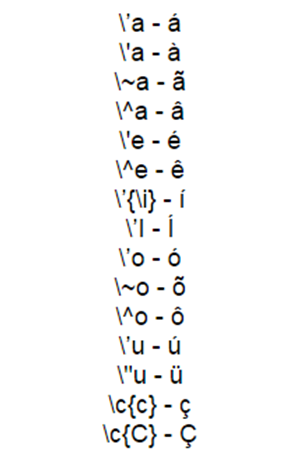
\includegraphics[scale=1.0]{USPSC-img/USPSC-AcentuacaoLaTeX.png} \\
	Fonte: \citeonline{comandos}
	\end{center}	
\end{figure}

\chapter{Símbolos úteis em \LaTeX}
\begin{figure}[H]
	\begin{center}
		\caption{\label{fig_anexoc}Símbolos úteis em \LaTeX}
		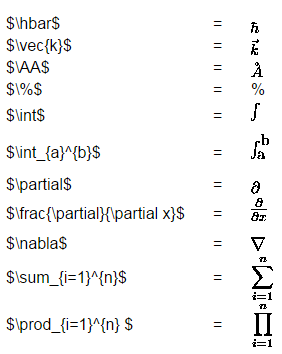
\includegraphics[scale=1.0]{USPSC-img/USPSC-SimbolosUteis.png} \\
		Fonte: \citeonline{comandos}
	\end{center}	
\end{figure}


\chapter{Letras gregas em \LaTeX}
\begin{figure}[H]
	\begin{center}
		\caption{\label{fig_anexod}Letras gregas em \LaTeX}
		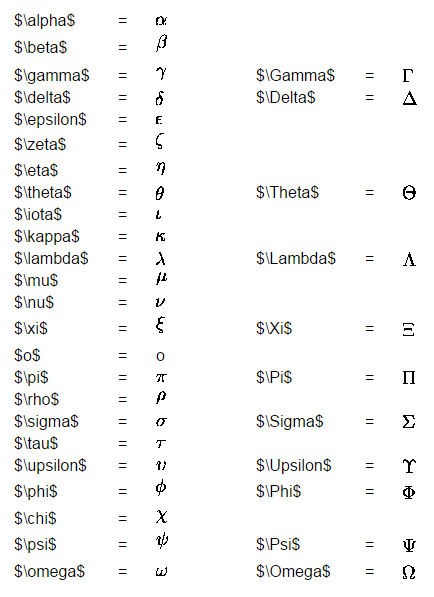
\includegraphics[scale=1.0]{USPSC-img/USPSC-LetrasGregas.png} \\
		Fonte: \citeonline{comandos}
	\end{center}	
\end{figure}

\end{anexosenv}


%---------------------------------------------------------------------
% INDICE REMISSIVO
%--------------------------------------------------------------------
%%% USPSC-IndicexRemissivosTutorial.tex
% ---
% Inicia os Índices Remissivos
% ---
%---------------------------------------------------------------------
% INDICE REMISSIVO
%--------------------------------------------------------------------
\phantompart
\printindex
%---------------------------------------------------------------------

\phantompart
\printindex
%---------------------------------------------------------------------


\end{document}
